% Options for packages loaded elsewhere
\PassOptionsToPackage{unicode}{hyperref}
\PassOptionsToPackage{hyphens}{url}
\PassOptionsToPackage{dvipsnames,svgnames,x11names}{xcolor}
%
\documentclass[
  letterpaper,
  DIV=11,
  numbers=noendperiod,
  titlepage]{scrartcl}

\usepackage{amsmath,amssymb}
\usepackage{iftex}
\ifPDFTeX
  \usepackage[T1]{fontenc}
  \usepackage[utf8]{inputenc}
  \usepackage{textcomp} % provide euro and other symbols
\else % if luatex or xetex
  \usepackage{unicode-math}
  \defaultfontfeatures{Scale=MatchLowercase}
  \defaultfontfeatures[\rmfamily]{Ligatures=TeX,Scale=1}
\fi
\usepackage{lmodern}
\ifPDFTeX\else  
    % xetex/luatex font selection
\fi
% Use upquote if available, for straight quotes in verbatim environments
\IfFileExists{upquote.sty}{\usepackage{upquote}}{}
\IfFileExists{microtype.sty}{% use microtype if available
  \usepackage[]{microtype}
  \UseMicrotypeSet[protrusion]{basicmath} % disable protrusion for tt fonts
}{}
\makeatletter
\@ifundefined{KOMAClassName}{% if non-KOMA class
  \IfFileExists{parskip.sty}{%
    \usepackage{parskip}
  }{% else
    \setlength{\parindent}{0pt}
    \setlength{\parskip}{6pt plus 2pt minus 1pt}}
}{% if KOMA class
  \KOMAoptions{parskip=half}}
\makeatother
\usepackage{xcolor}
\usepackage[top=20mm,bottom=5mm]{geometry}
\setlength{\emergencystretch}{3em} % prevent overfull lines
\setcounter{secnumdepth}{-\maxdimen} % remove section numbering
% Make \paragraph and \subparagraph free-standing
\ifx\paragraph\undefined\else
  \let\oldparagraph\paragraph
  \renewcommand{\paragraph}[1]{\oldparagraph{#1}\mbox{}}
\fi
\ifx\subparagraph\undefined\else
  \let\oldsubparagraph\subparagraph
  \renewcommand{\subparagraph}[1]{\oldsubparagraph{#1}\mbox{}}
\fi


\providecommand{\tightlist}{%
  \setlength{\itemsep}{0pt}\setlength{\parskip}{0pt}}\usepackage{longtable,booktabs,array}
\usepackage{calc} % for calculating minipage widths
% Correct order of tables after \paragraph or \subparagraph
\usepackage{etoolbox}
\makeatletter
\patchcmd\longtable{\par}{\if@noskipsec\mbox{}\fi\par}{}{}
\makeatother
% Allow footnotes in longtable head/foot
\IfFileExists{footnotehyper.sty}{\usepackage{footnotehyper}}{\usepackage{footnote}}
\makesavenoteenv{longtable}
\usepackage{graphicx}
\makeatletter
\def\maxwidth{\ifdim\Gin@nat@width>\linewidth\linewidth\else\Gin@nat@width\fi}
\def\maxheight{\ifdim\Gin@nat@height>\textheight\textheight\else\Gin@nat@height\fi}
\makeatother
% Scale images if necessary, so that they will not overflow the page
% margins by default, and it is still possible to overwrite the defaults
% using explicit options in \includegraphics[width, height, ...]{}
\setkeys{Gin}{width=\maxwidth,height=\maxheight,keepaspectratio}
% Set default figure placement to htbp
\makeatletter
\def\fps@figure{htbp}
\makeatother

\usepackage{booktabs}
\usepackage{longtable}
\usepackage{array}
\usepackage{multirow}
\usepackage{wrapfig}
\usepackage{float}
\usepackage{colortbl}
\usepackage{pdflscape}
\usepackage{tabu}
\usepackage{threeparttable}
\usepackage{threeparttablex}
\usepackage[normalem]{ulem}
\usepackage{makecell}
\usepackage{xcolor}
\usepackage{typearea}
\usepackage{caption}
\captionsetup{font=tiny}
\KOMAoption{captions}{tableheading}
\makeatletter
\makeatother
\makeatletter
\makeatother
\makeatletter
\@ifpackageloaded{caption}{}{\usepackage{caption}}
\AtBeginDocument{%
\ifdefined\contentsname
  \renewcommand*\contentsname{Table of contents}
\else
  \newcommand\contentsname{Table of contents}
\fi
\ifdefined\listfigurename
  \renewcommand*\listfigurename{List of Figures}
\else
  \newcommand\listfigurename{List of Figures}
\fi
\ifdefined\listtablename
  \renewcommand*\listtablename{List of Tables}
\else
  \newcommand\listtablename{List of Tables}
\fi
\ifdefined\figurename
  \renewcommand*\figurename{Figure}
\else
  \newcommand\figurename{Figure}
\fi
\ifdefined\tablename
  \renewcommand*\tablename{Table}
\else
  \newcommand\tablename{Table}
\fi
}
\@ifpackageloaded{float}{}{\usepackage{float}}
\floatstyle{ruled}
\@ifundefined{c@chapter}{\newfloat{codelisting}{h}{lop}}{\newfloat{codelisting}{h}{lop}[chapter]}
\floatname{codelisting}{Listing}
\newcommand*\listoflistings{\listof{codelisting}{List of Listings}}
\makeatother
\makeatletter
\@ifpackageloaded{caption}{}{\usepackage{caption}}
\@ifpackageloaded{subcaption}{}{\usepackage{subcaption}}
\makeatother
\makeatletter
\@ifpackageloaded{tcolorbox}{}{\usepackage[skins,breakable]{tcolorbox}}
\makeatother
\makeatletter
\@ifundefined{shadecolor}{\definecolor{shadecolor}{rgb}{.97, .97, .97}}
\makeatother
\makeatletter
\makeatother
\makeatletter
\makeatother
\ifLuaTeX
  \usepackage{selnolig}  % disable illegal ligatures
\fi
\IfFileExists{bookmark.sty}{\usepackage{bookmark}}{\usepackage{hyperref}}
\IfFileExists{xurl.sty}{\usepackage{xurl}}{} % add URL line breaks if available
\urlstyle{same} % disable monospaced font for URLs
\hypersetup{
  pdftitle={Simulation Result For Two-Level Slope Model With High Prevalence},
  pdfauthor={Shafayet Khan Shafee},
  colorlinks=true,
  linkcolor={blue},
  filecolor={Maroon},
  citecolor={Blue},
  urlcolor={Blue},
  pdfcreator={LaTeX via pandoc}}

\title{Simulation Result For Two-Level Slope Model With High Prevalence}
\usepackage{etoolbox}
\makeatletter
\providecommand{\subtitle}[1]
\author{Shafayet Khan Shafee}
\date{03 September 2023}

\begin{document}
\maketitle
\ifdefined\Shaded\renewenvironment{Shaded}{\begin{tcolorbox}[frame hidden, interior hidden, breakable, enhanced, boxrule=0pt, sharp corners, borderline west={3pt}{0pt}{shadecolor}]}{\end{tcolorbox}}\fi

\newpage

\hypertarget{histograms-for-logwidehatmor-when-first-quartile-of-x-is-used}{%
\section{\texorpdfstring{Histograms for \(log(\widehat{MOR})\) when
First Quartile of \(X\) is
used}{Histograms for log(\textbackslash widehat\{MOR\}) when First Quartile of X is used}}\label{histograms-for-logwidehatmor-when-first-quartile-of-x-is-used}}

\vspace{10mm}

\begin{figure}

\begin{minipage}[t]{0.05\linewidth}

{\centering 

\rotatebox[origin=br]{90}{\tiny Cluster Number 10}

}

\end{minipage}%
%
\begin{minipage}[t]{0.24\linewidth}

{\centering 

\raisebox{-\height}{

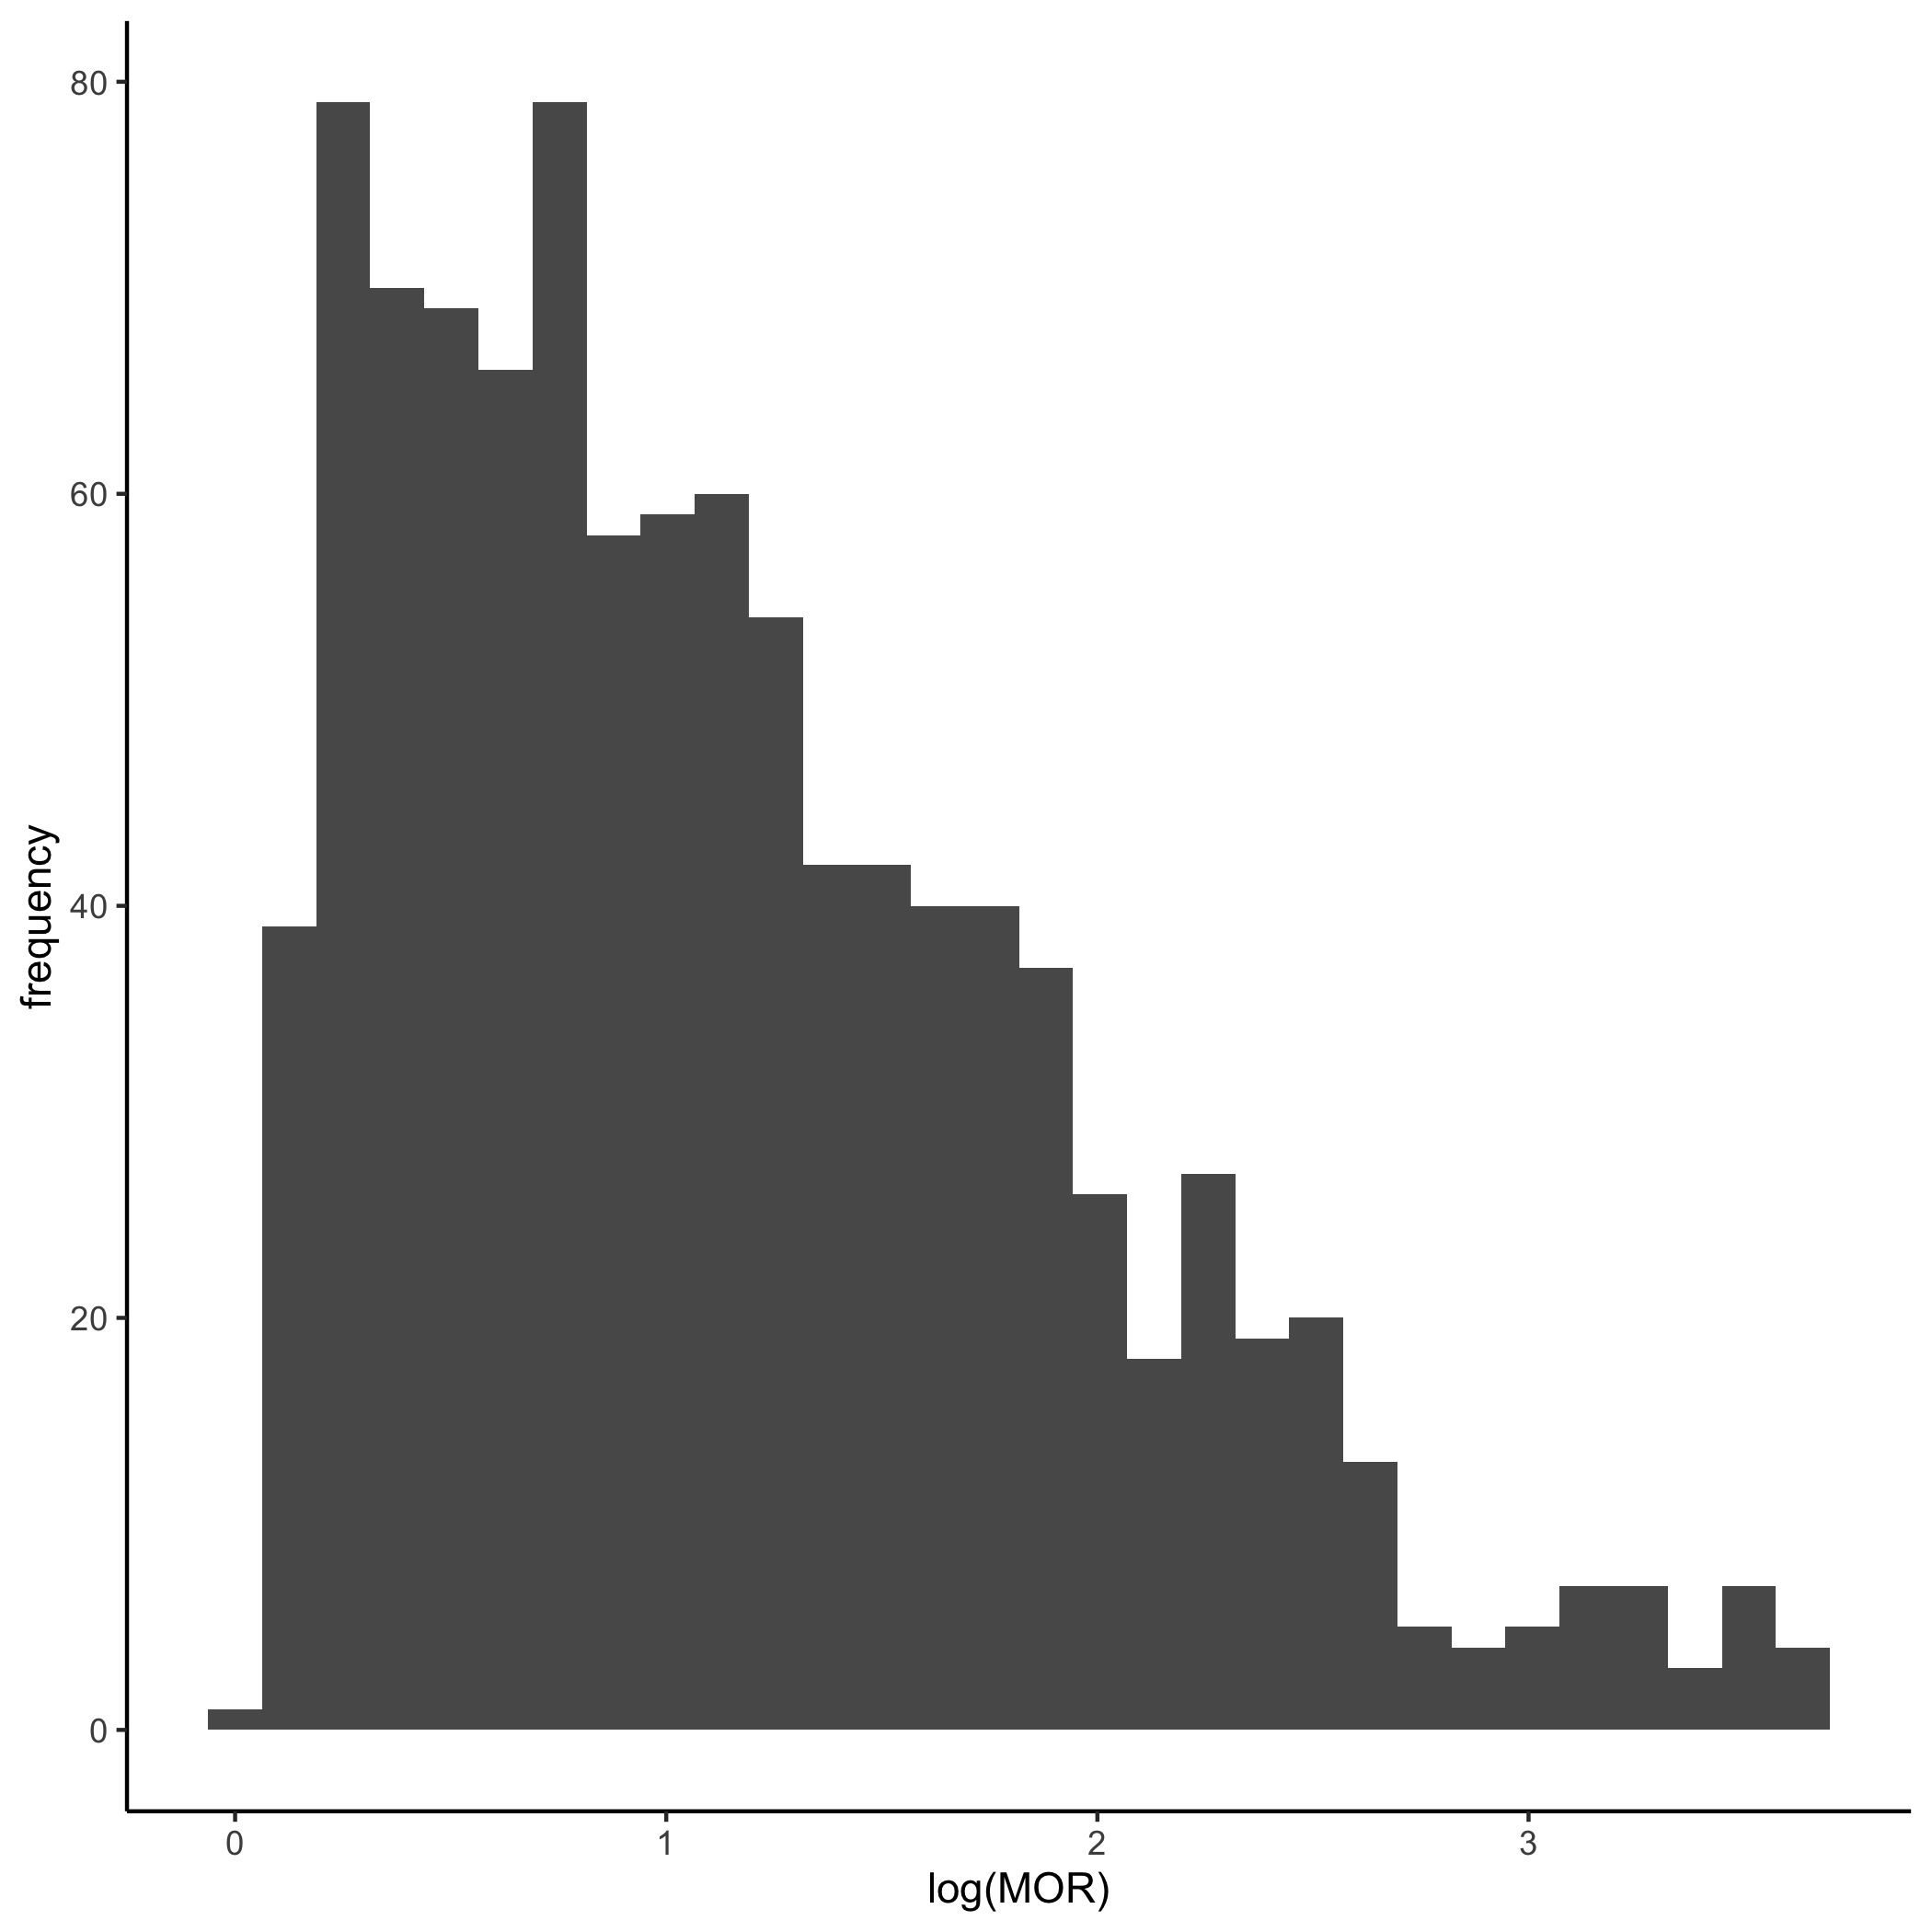
\includegraphics{../../plots/two-lvl-ran-slope/high-prev/hist_10_5_two_lvl_slp_high_prev_q1.png}

}

\caption{Cluster size 5}

}

\end{minipage}%
%
\begin{minipage}[t]{0.24\linewidth}

{\centering 

\raisebox{-\height}{

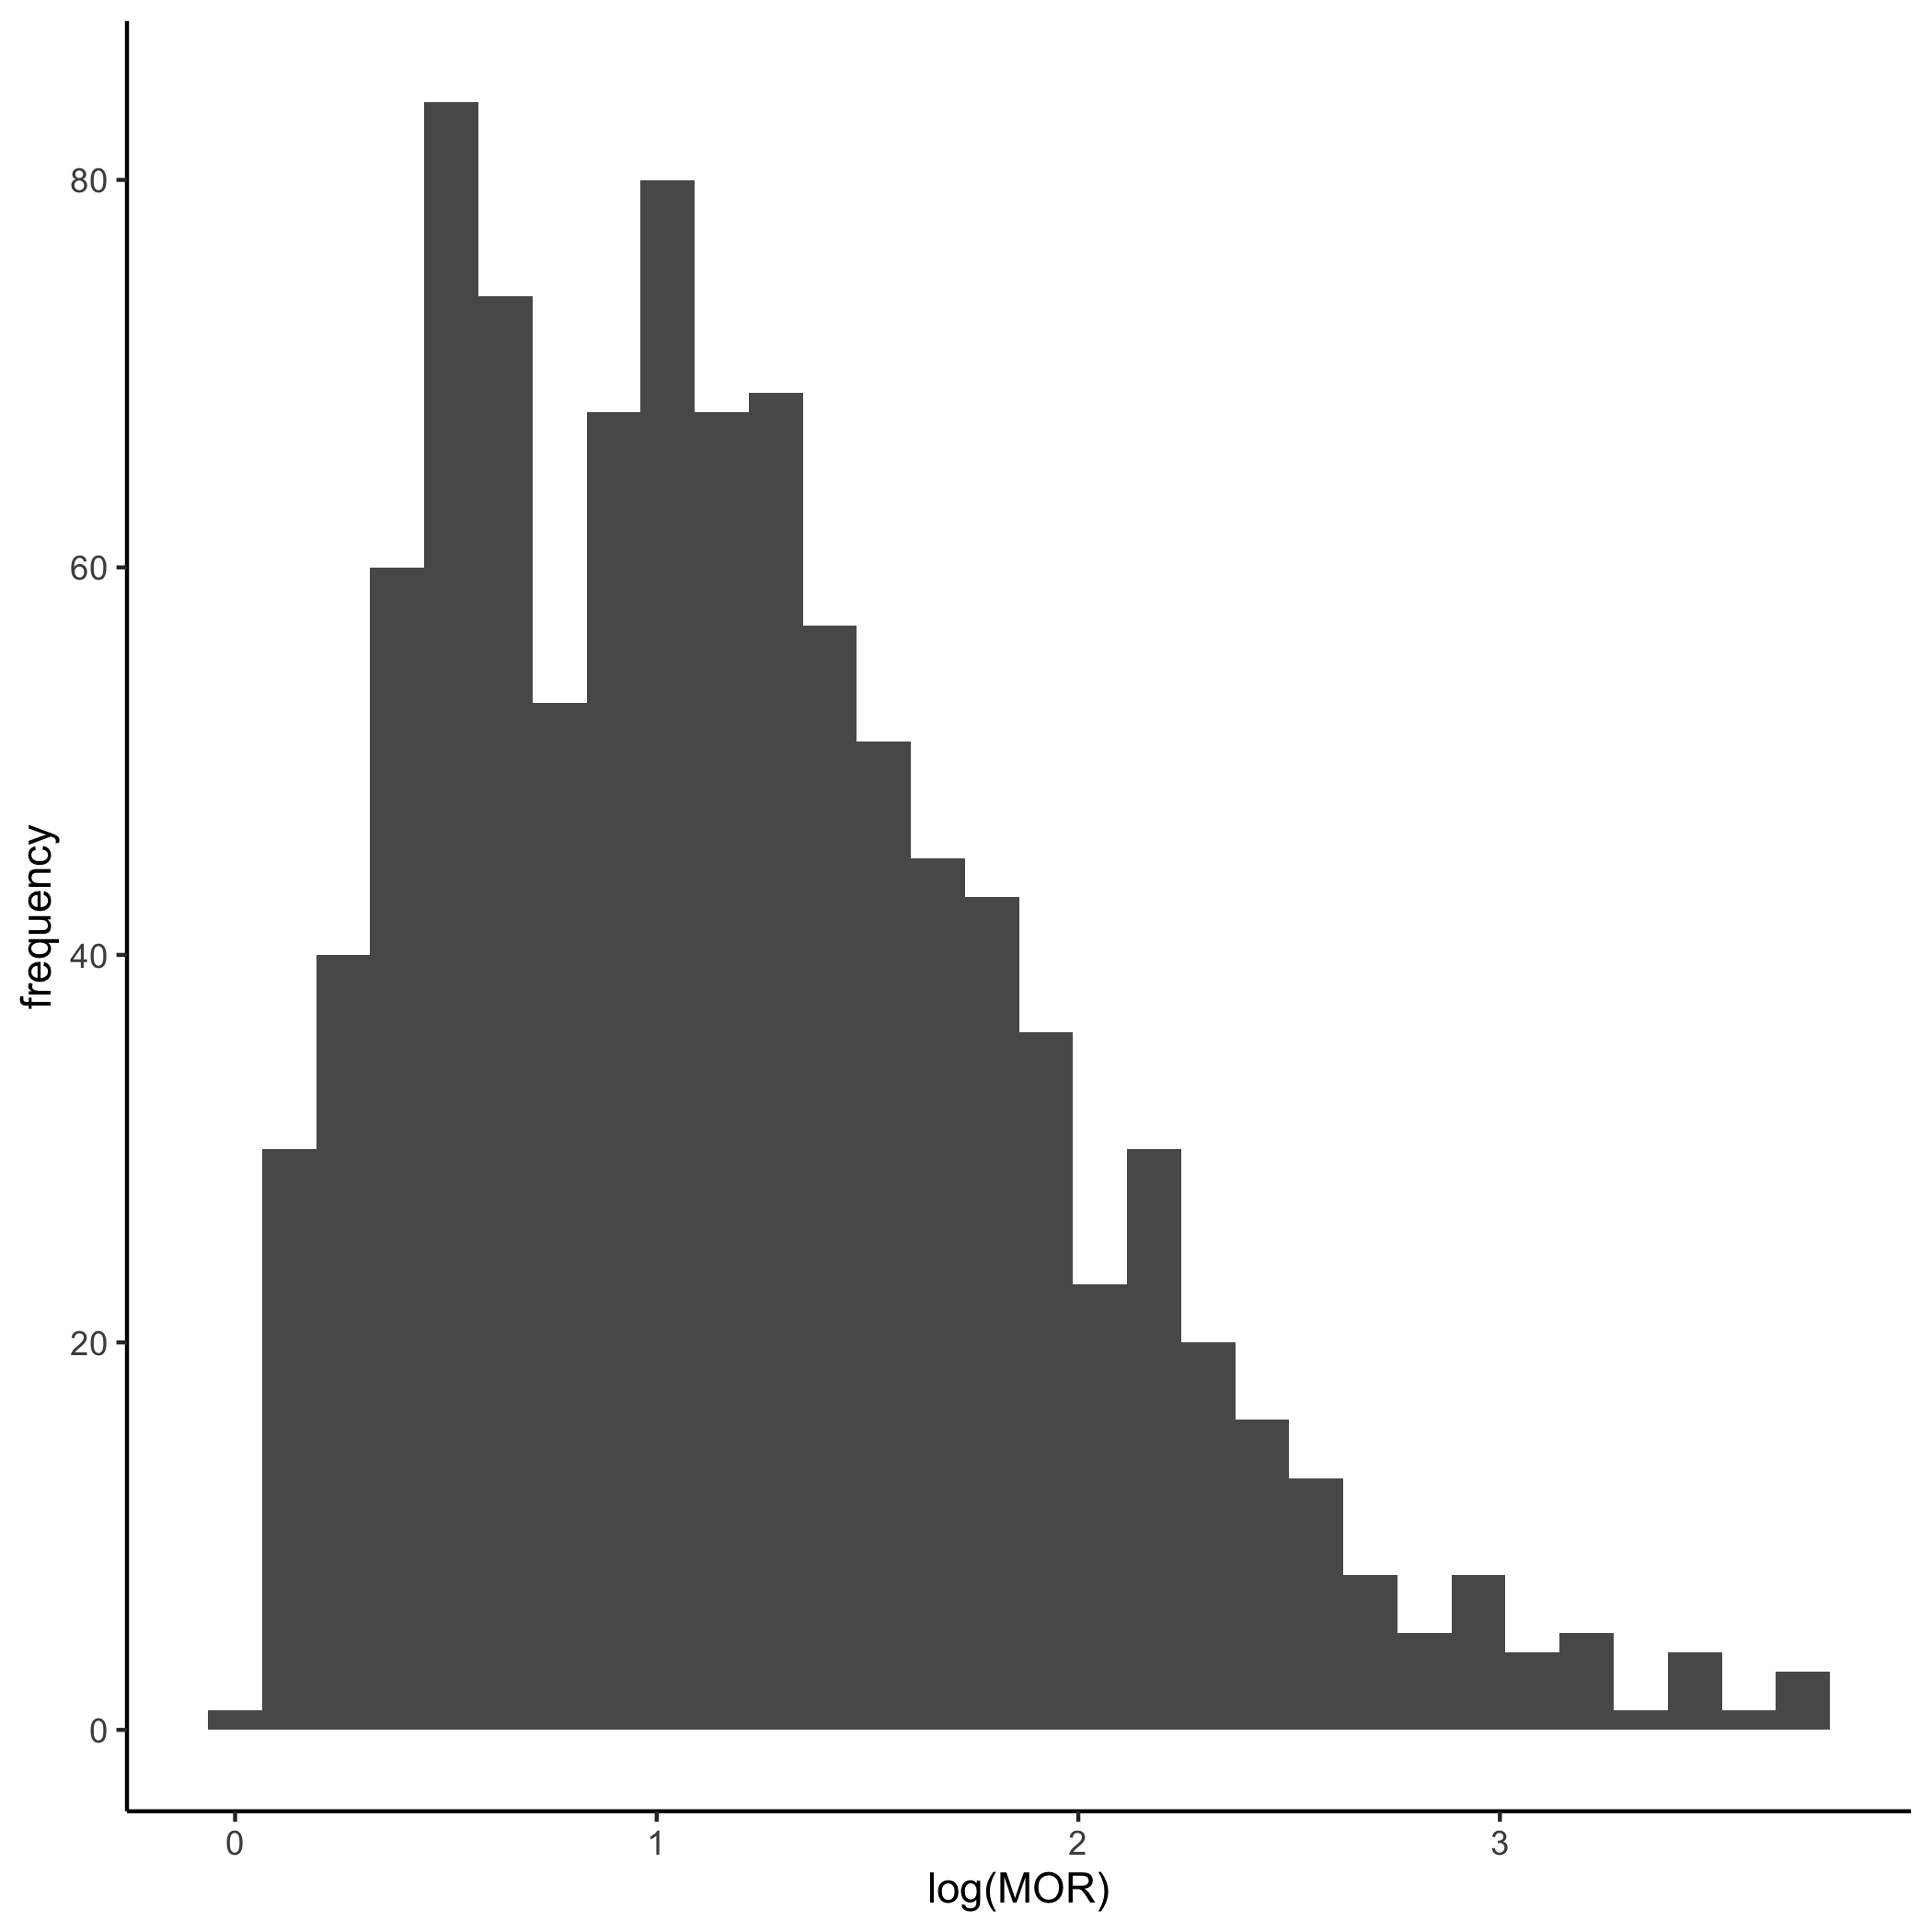
\includegraphics{../../plots/two-lvl-ran-slope/high-prev/hist_10_10_two_lvl_slp_high_prev_q1.png}

}

\caption{Cluster size 10}

}

\end{minipage}%
%
\begin{minipage}[t]{0.24\linewidth}

{\centering 

\raisebox{-\height}{

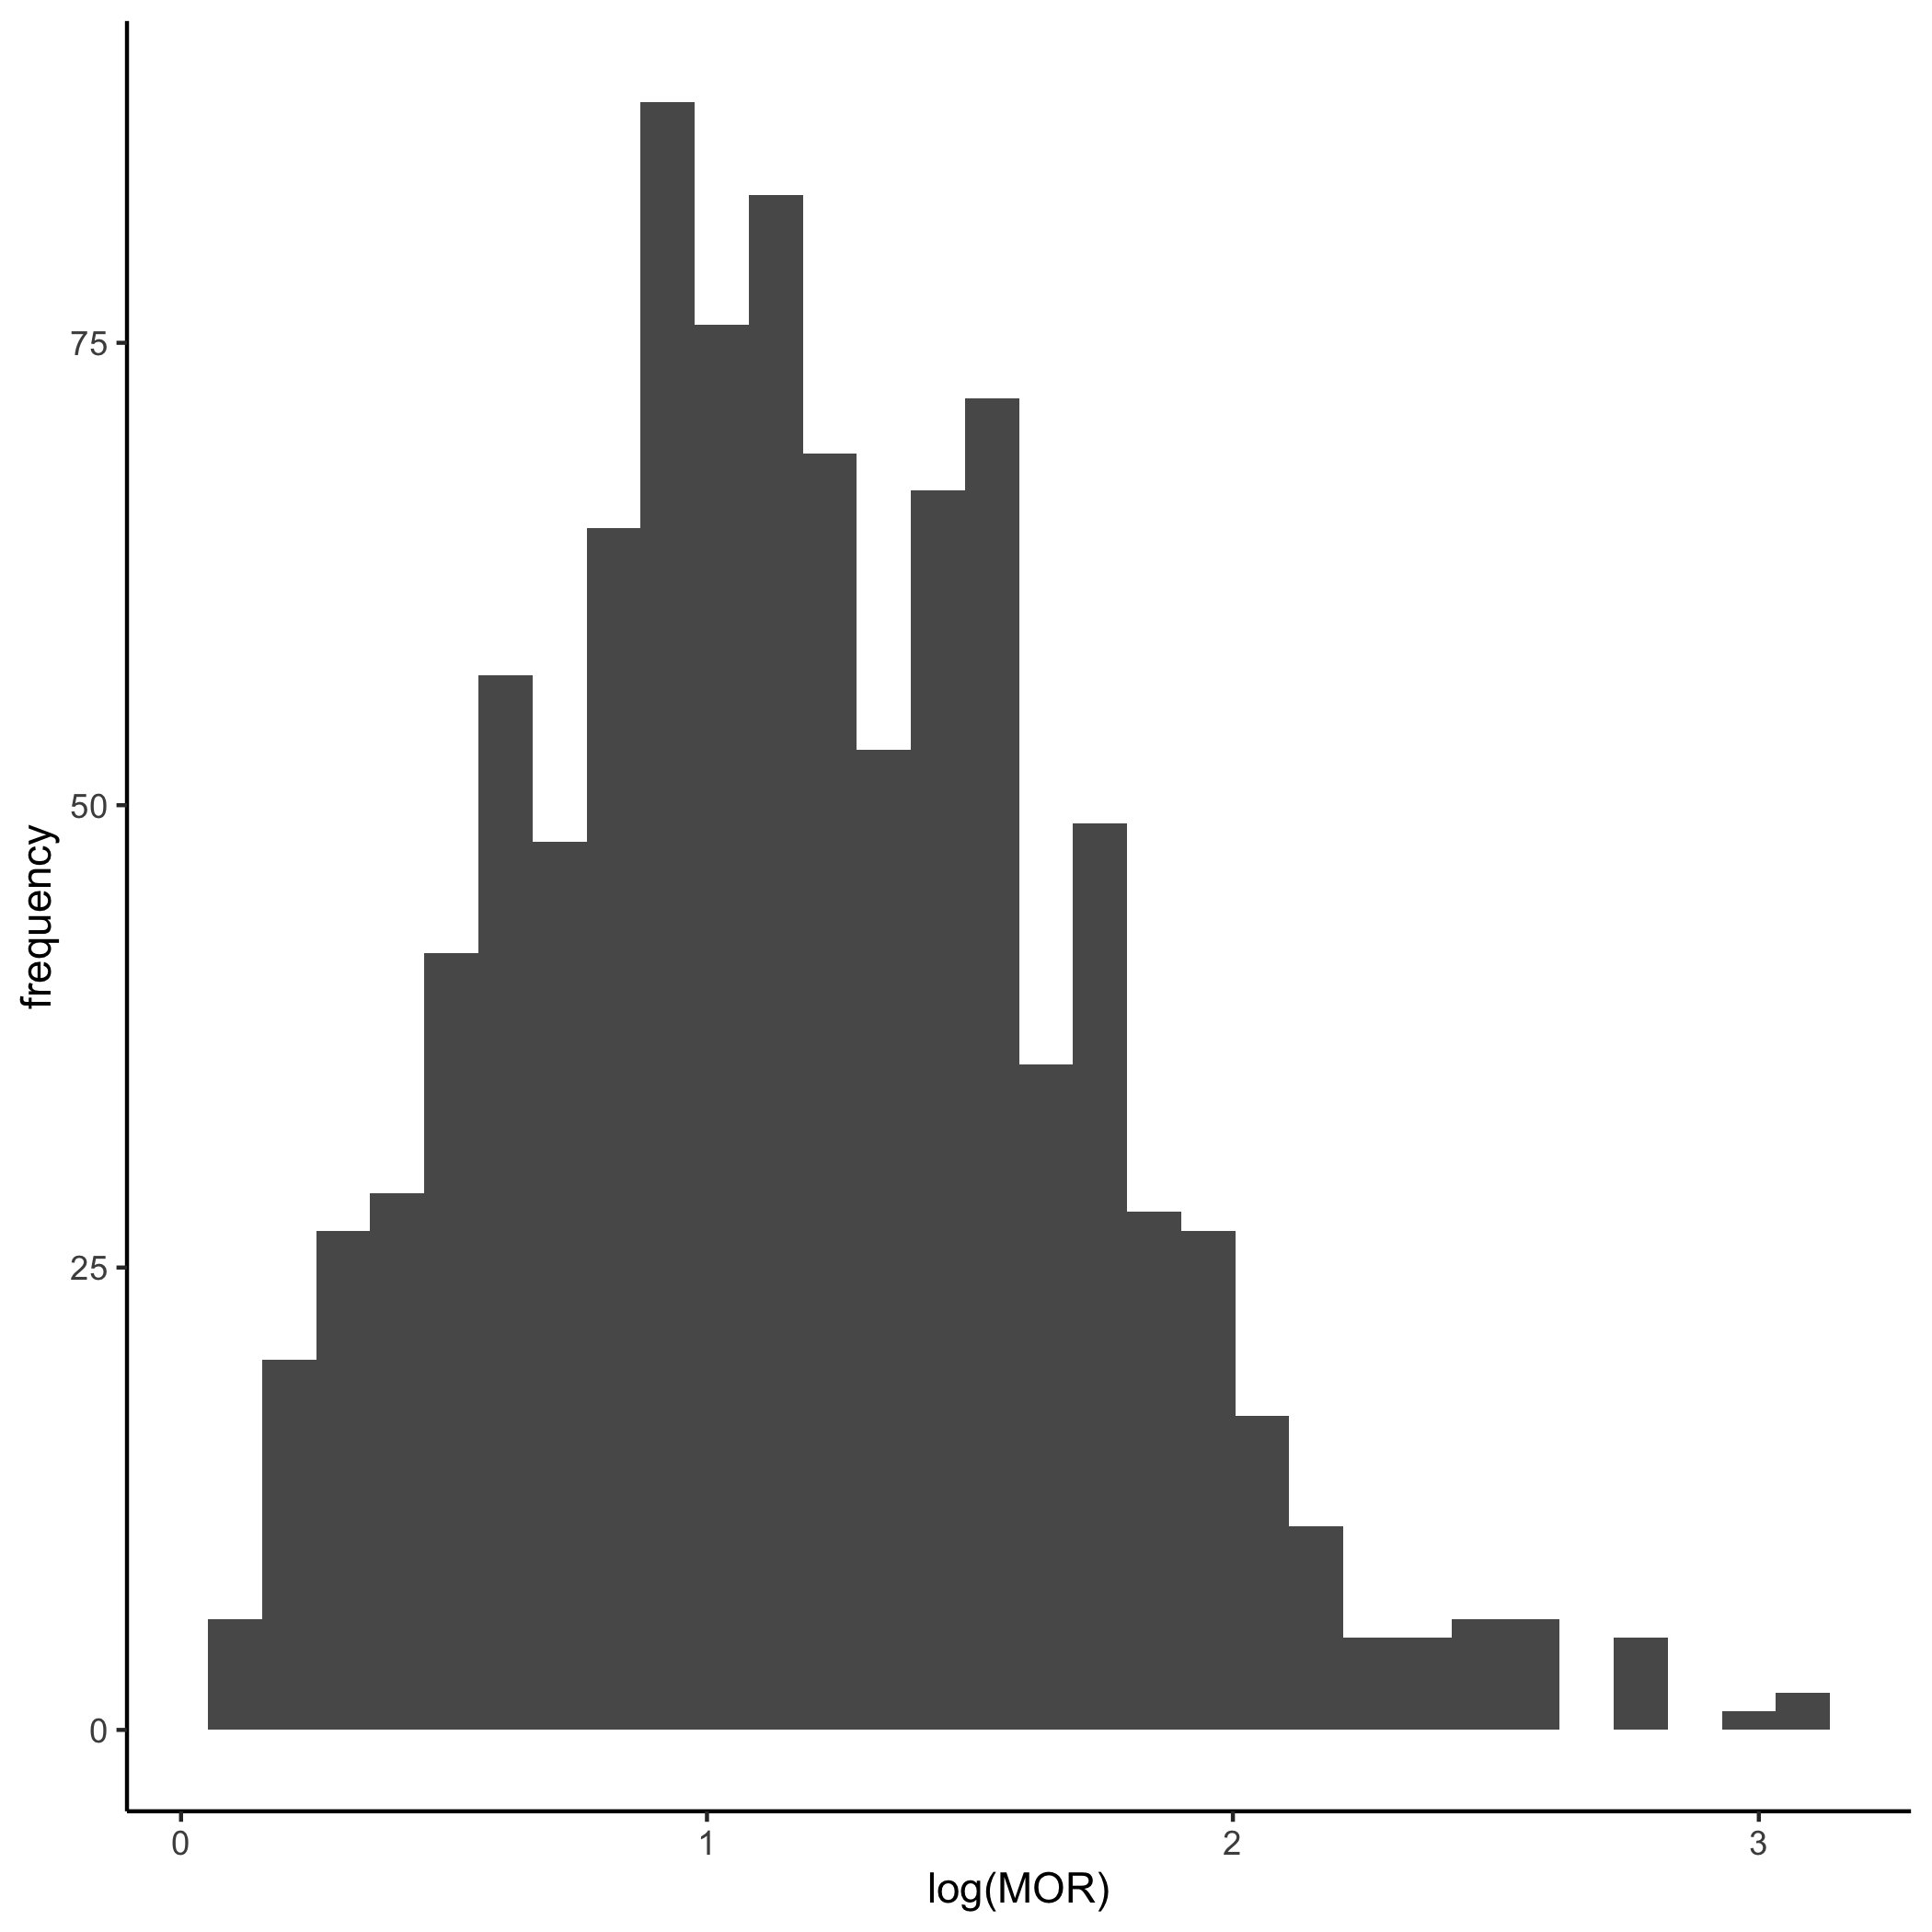
\includegraphics{../../plots/two-lvl-ran-slope/high-prev/hist_10_30_two_lvl_slp_high_prev_q1.png}

}

\caption{Cluster size 30}

}

\end{minipage}%
%
\begin{minipage}[t]{0.24\linewidth}

{\centering 

\raisebox{-\height}{

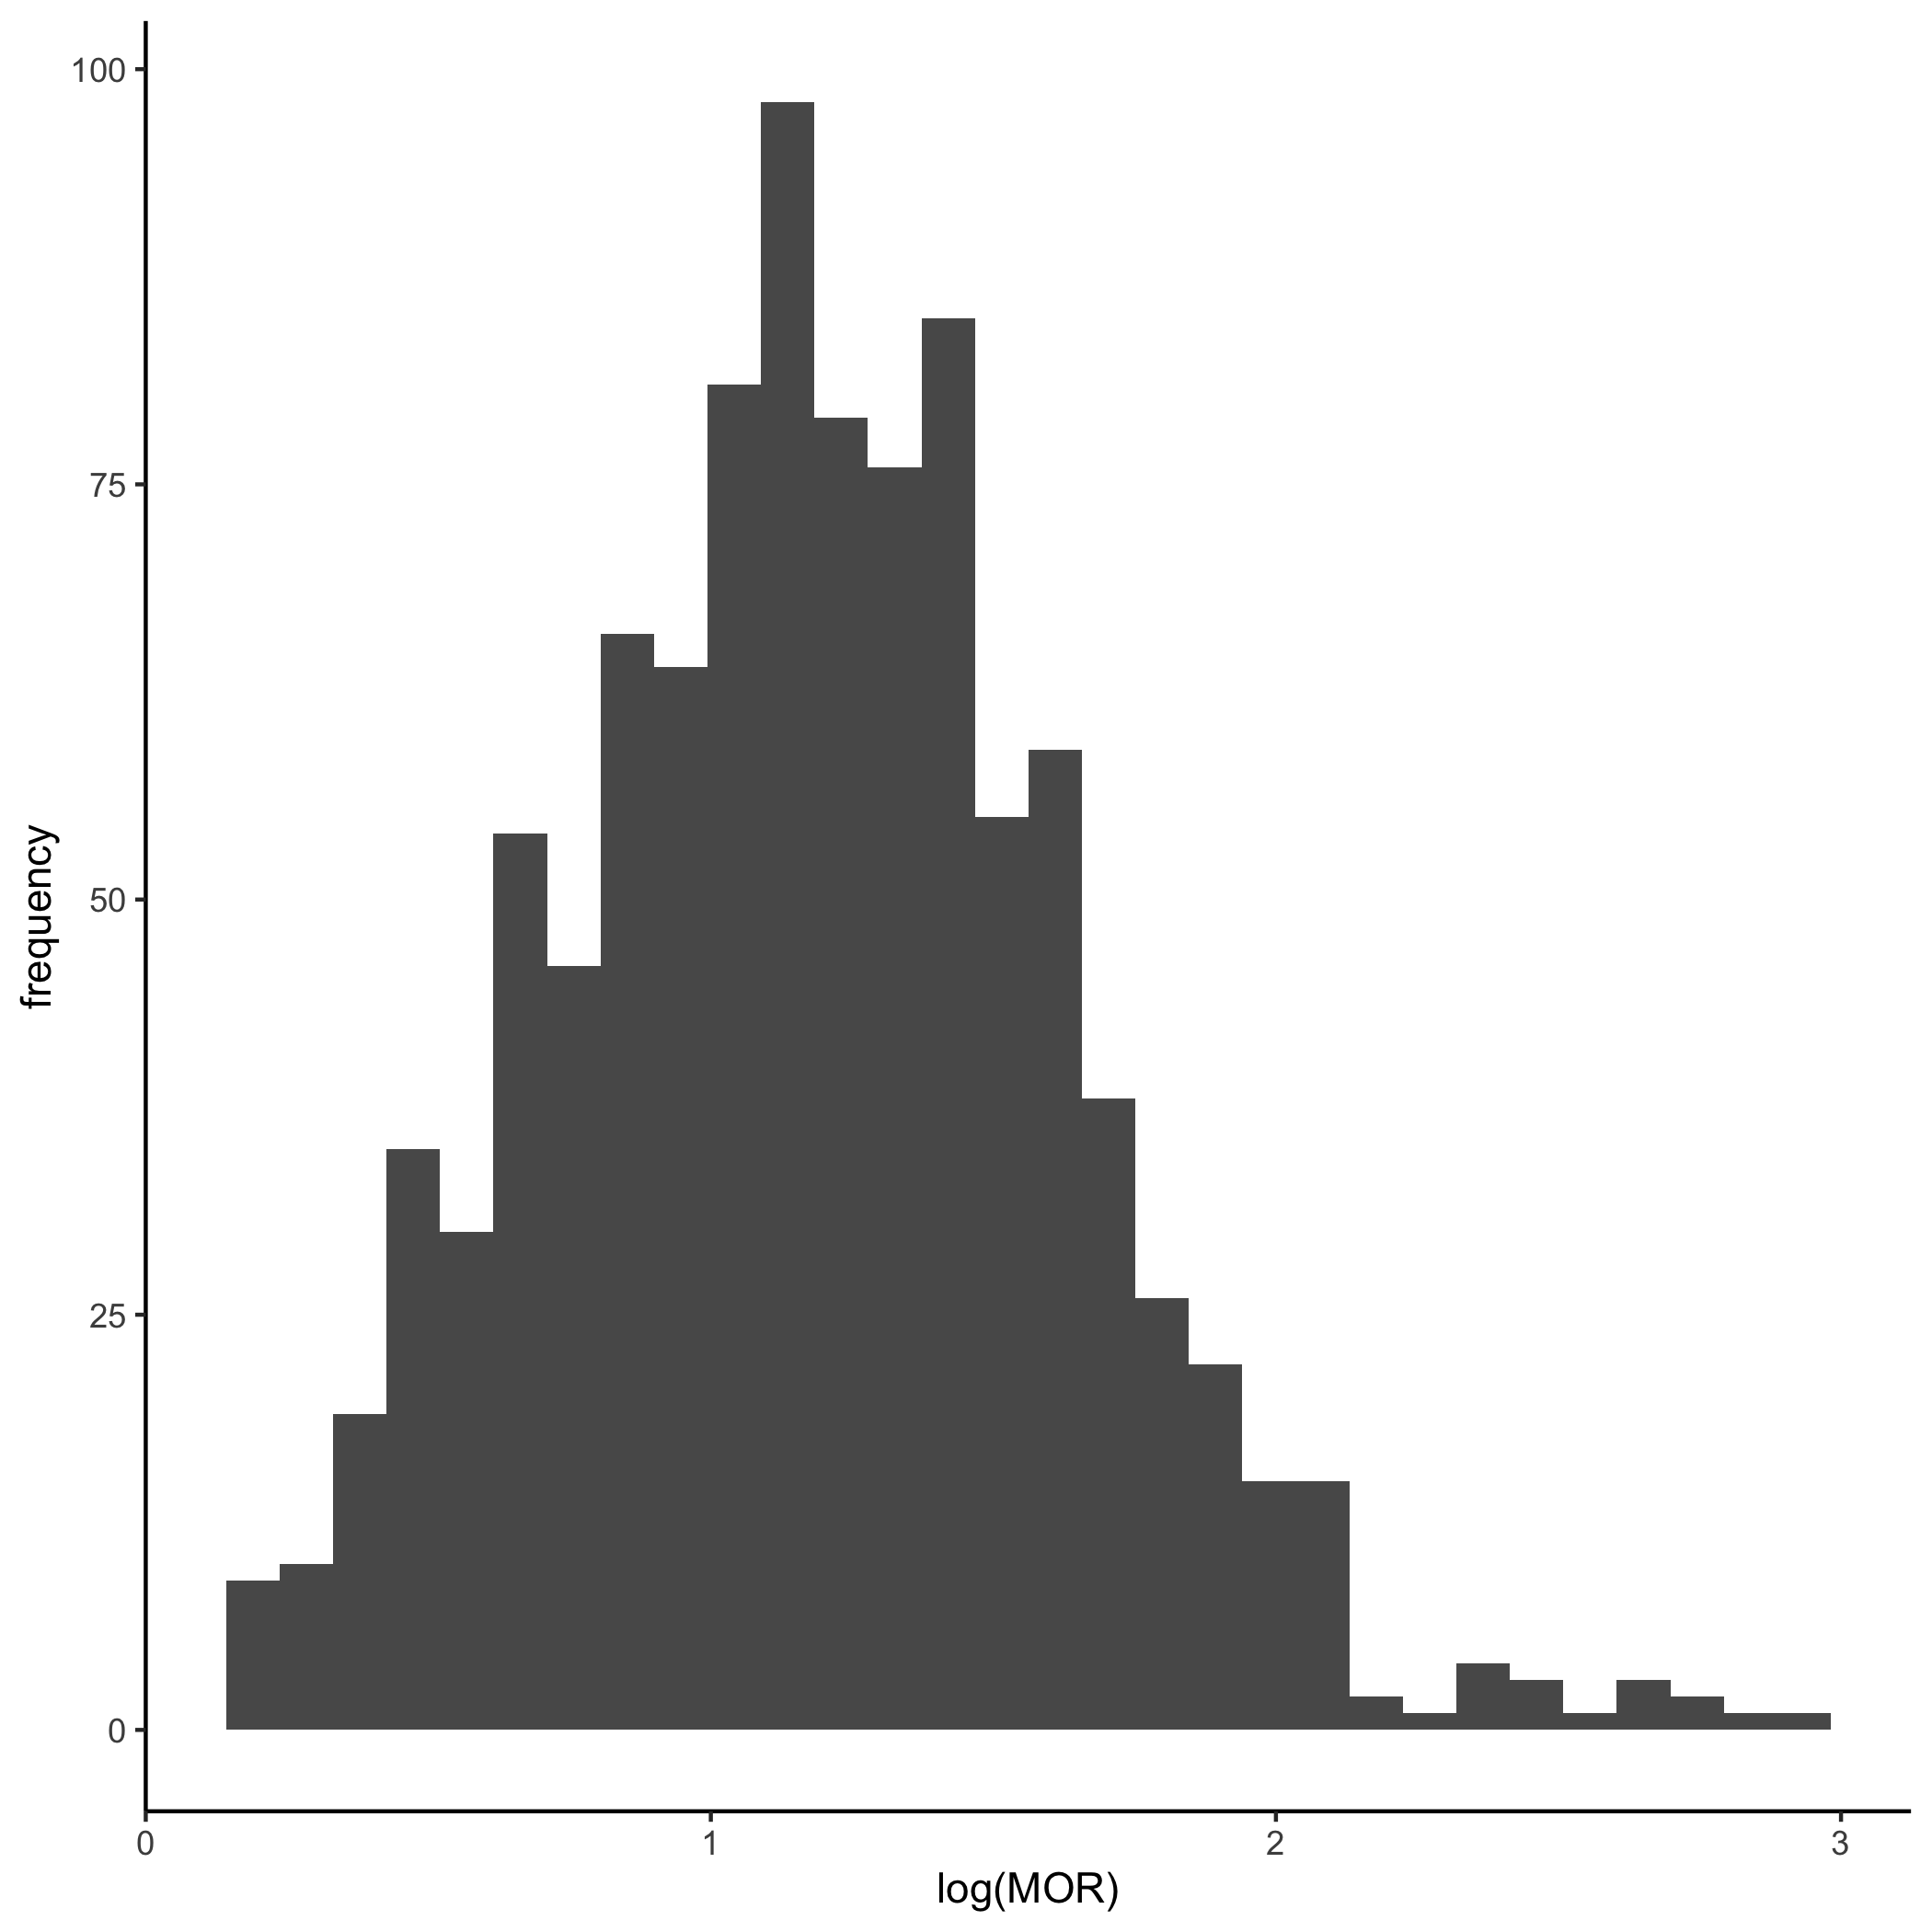
\includegraphics{../../plots/two-lvl-ran-slope/high-prev/hist_10_50_two_lvl_slp_high_prev_q1.png}

}

\caption{Cluster size 50}

}

\end{minipage}%
\newline
\begin{minipage}[t]{\linewidth}

{\centering 

~

}

\end{minipage}%
\newline
\begin{minipage}[t]{0.05\linewidth}

{\centering 

\rotatebox[origin=br]{90}{\tiny Cluster Number 30}

}

\end{minipage}%
%
\begin{minipage}[t]{0.24\linewidth}

{\centering 

\raisebox{-\height}{

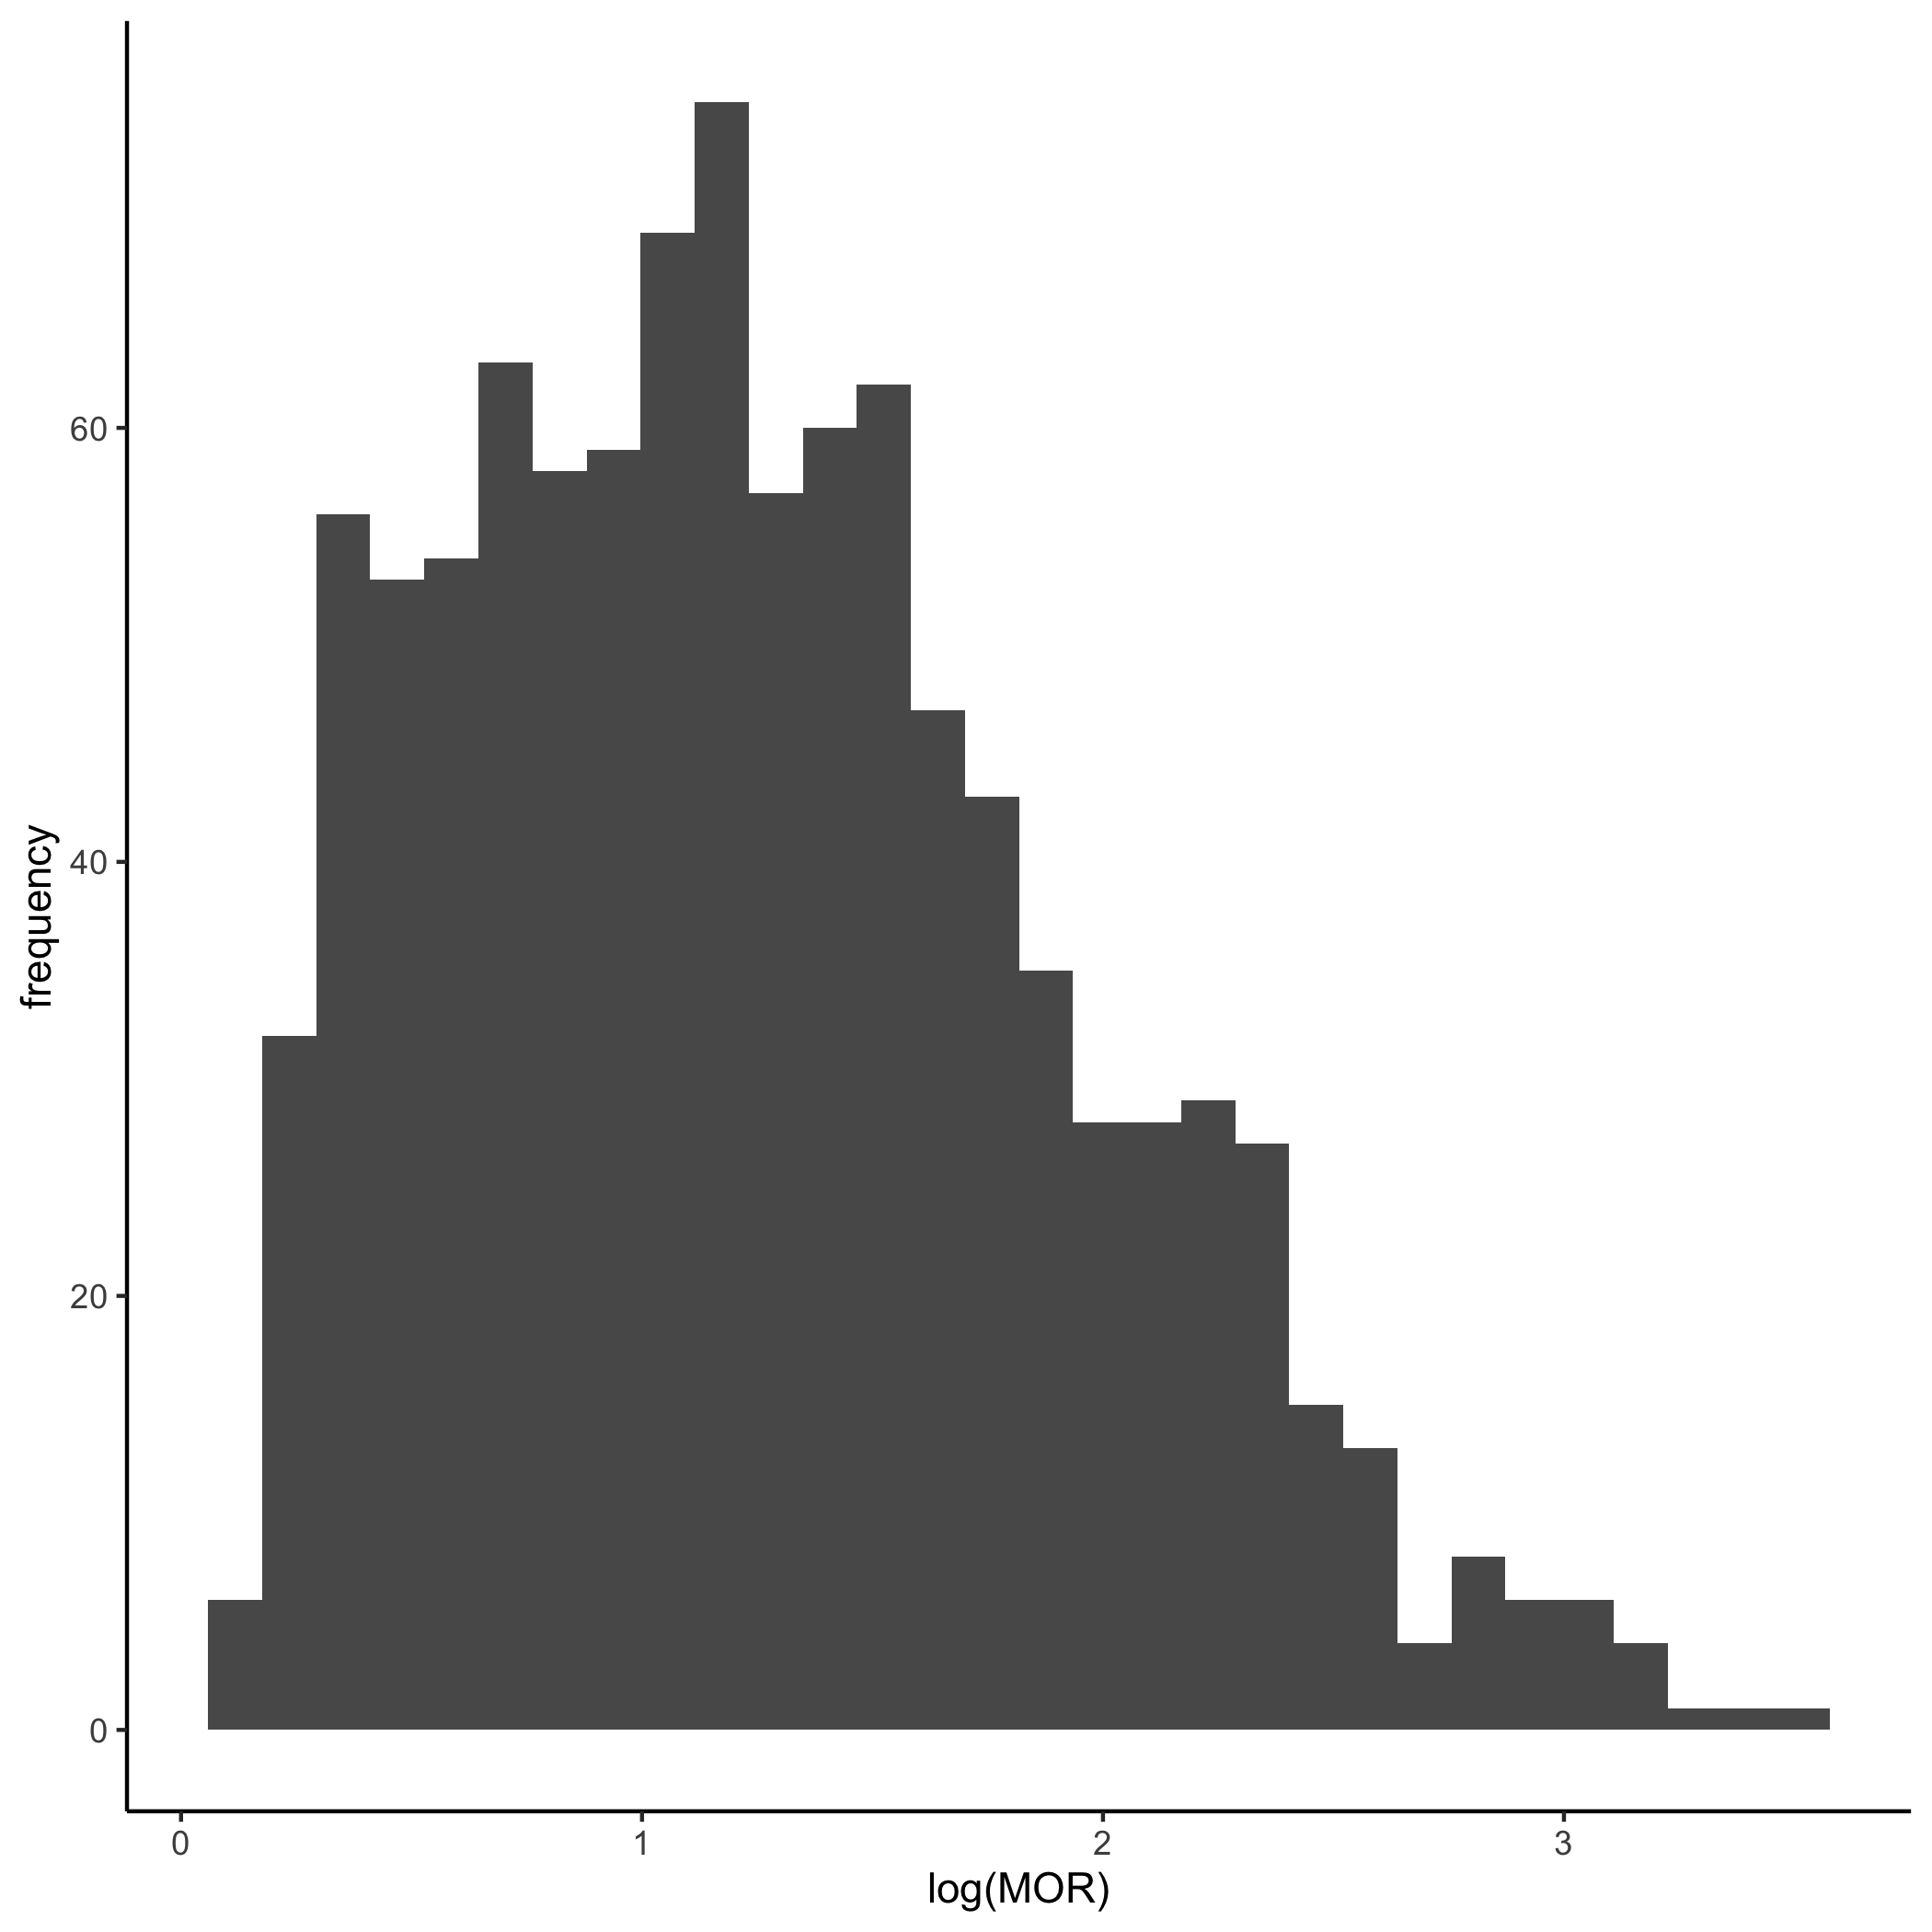
\includegraphics{../../plots/two-lvl-ran-slope/high-prev/hist_30_5_two_lvl_slp_high_prev_q1.png}

}

\caption{Cluster size 5}

}

\end{minipage}%
%
\begin{minipage}[t]{0.24\linewidth}

{\centering 

\raisebox{-\height}{

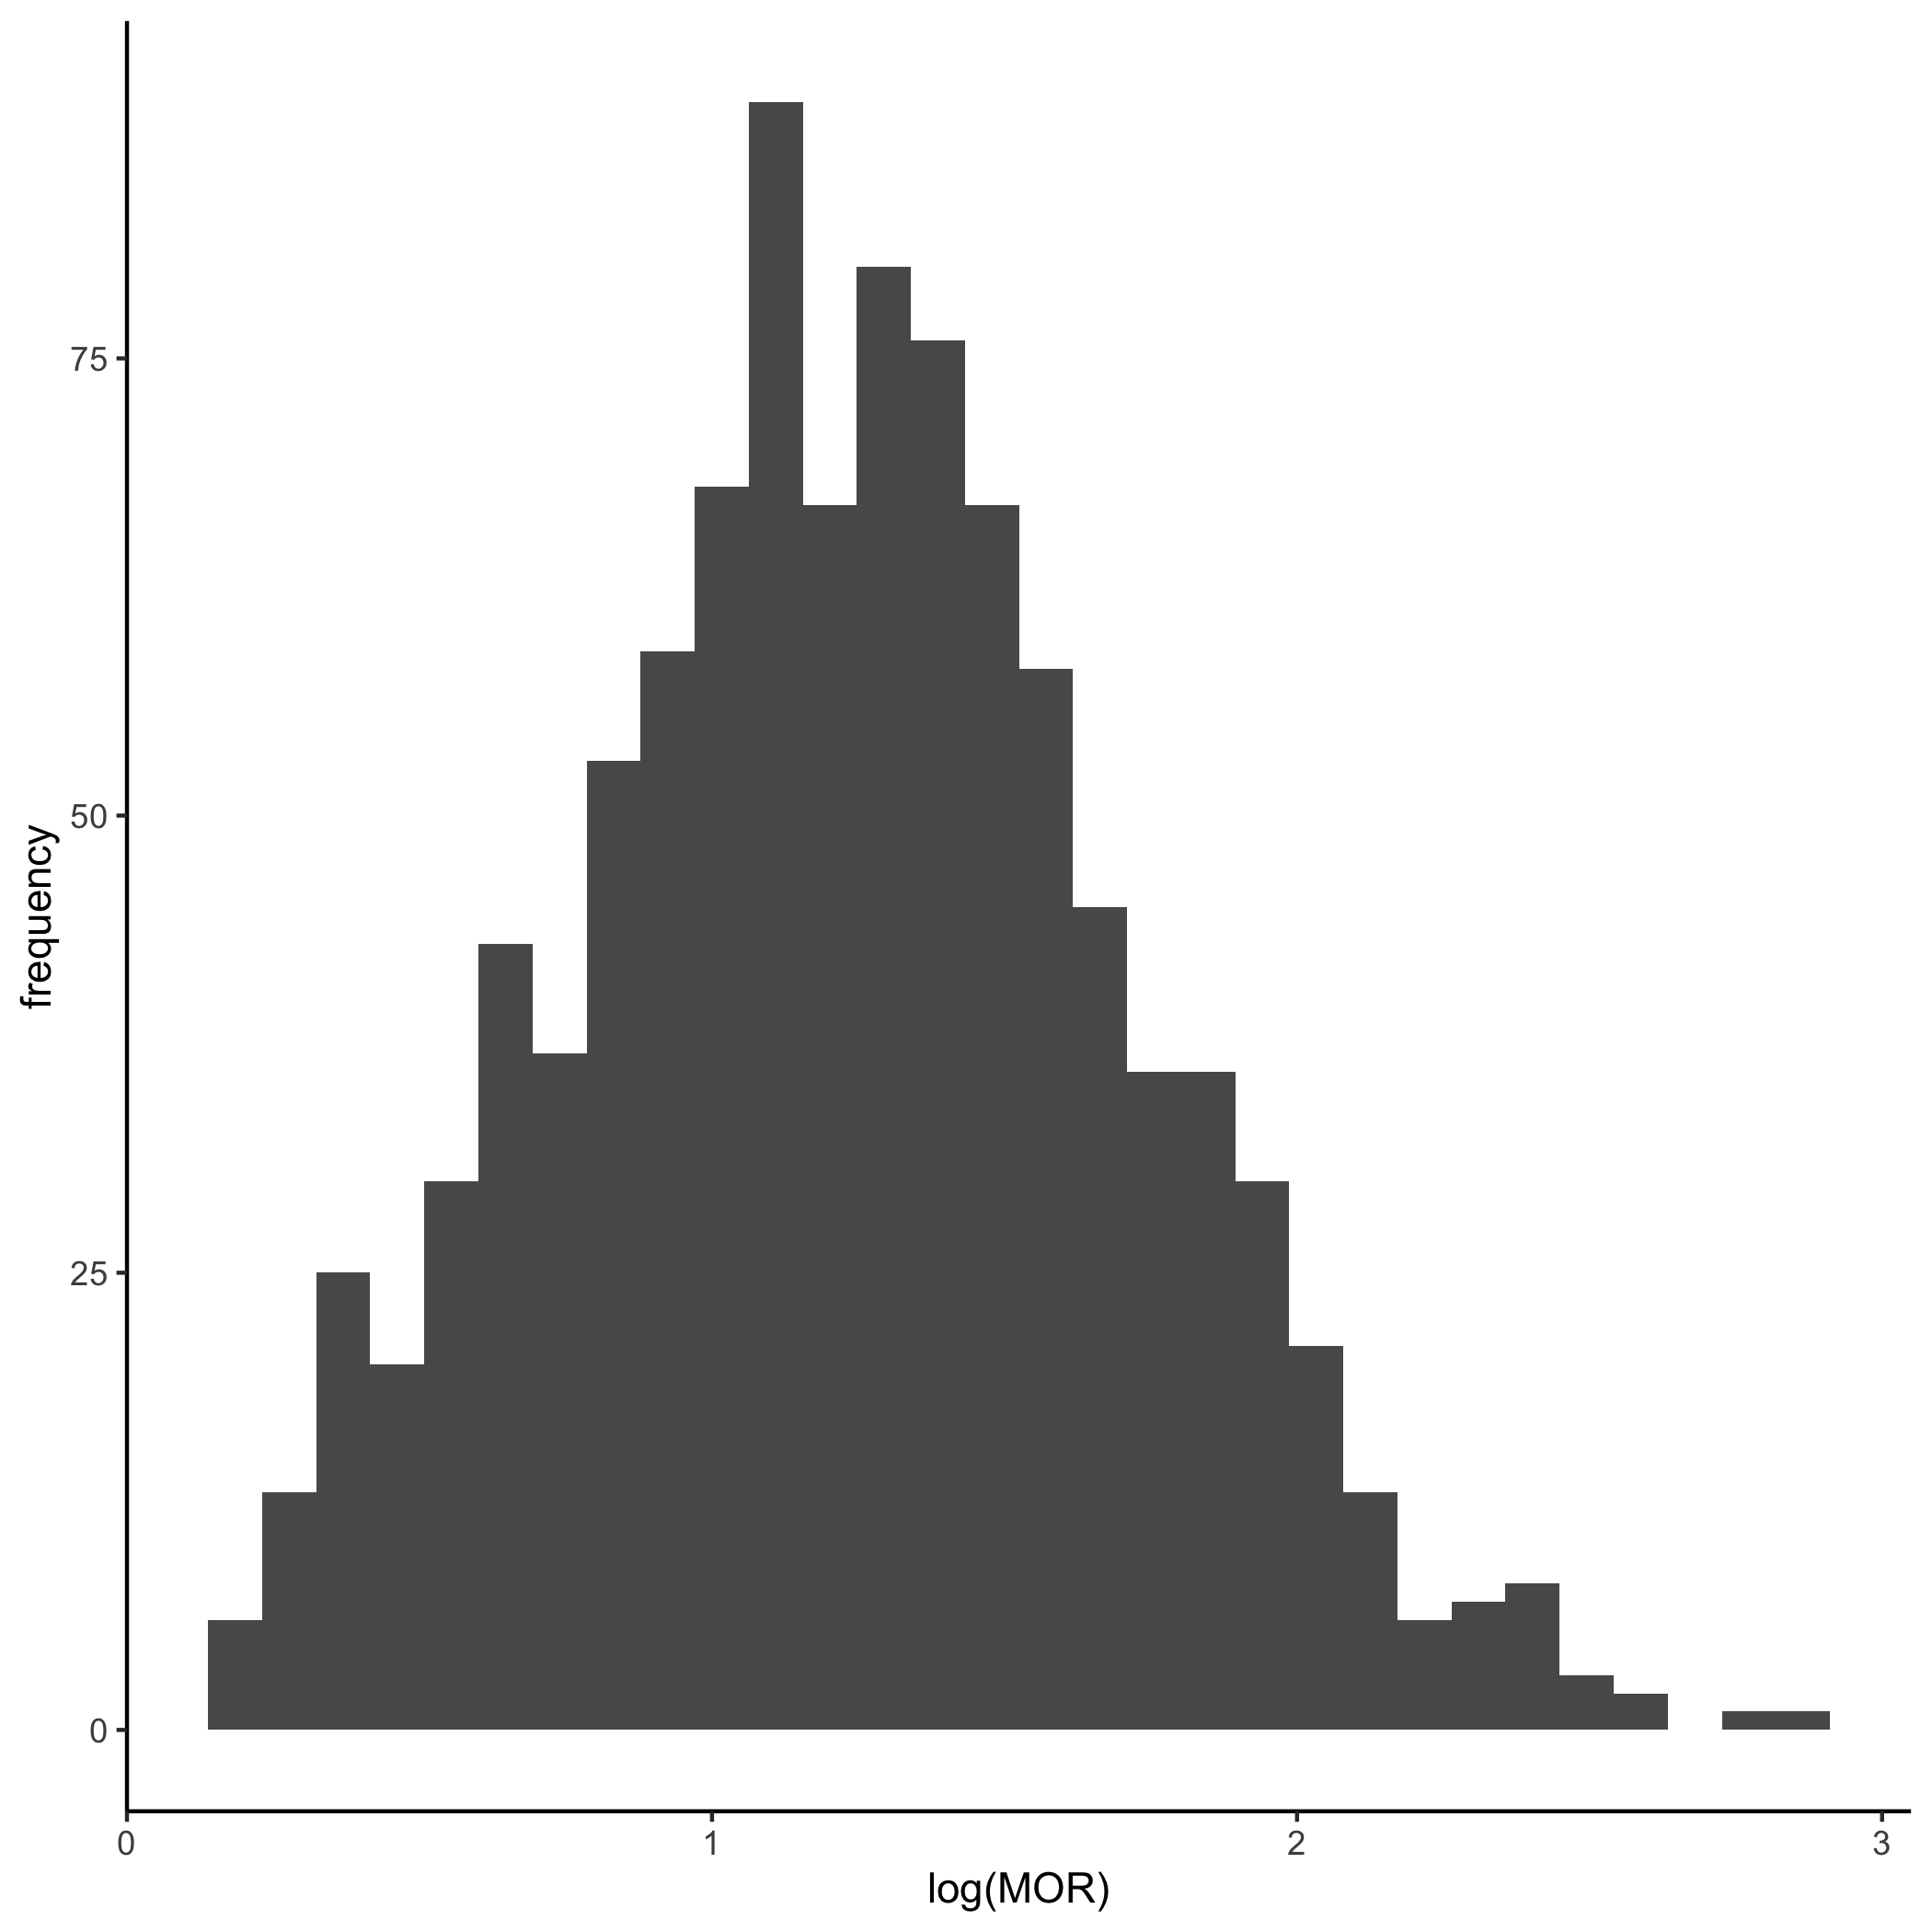
\includegraphics{../../plots/two-lvl-ran-slope/high-prev/hist_30_10_two_lvl_slp_high_prev_q1.png}

}

\caption{Cluster size 10}

}

\end{minipage}%
%
\begin{minipage}[t]{0.24\linewidth}

{\centering 

\raisebox{-\height}{

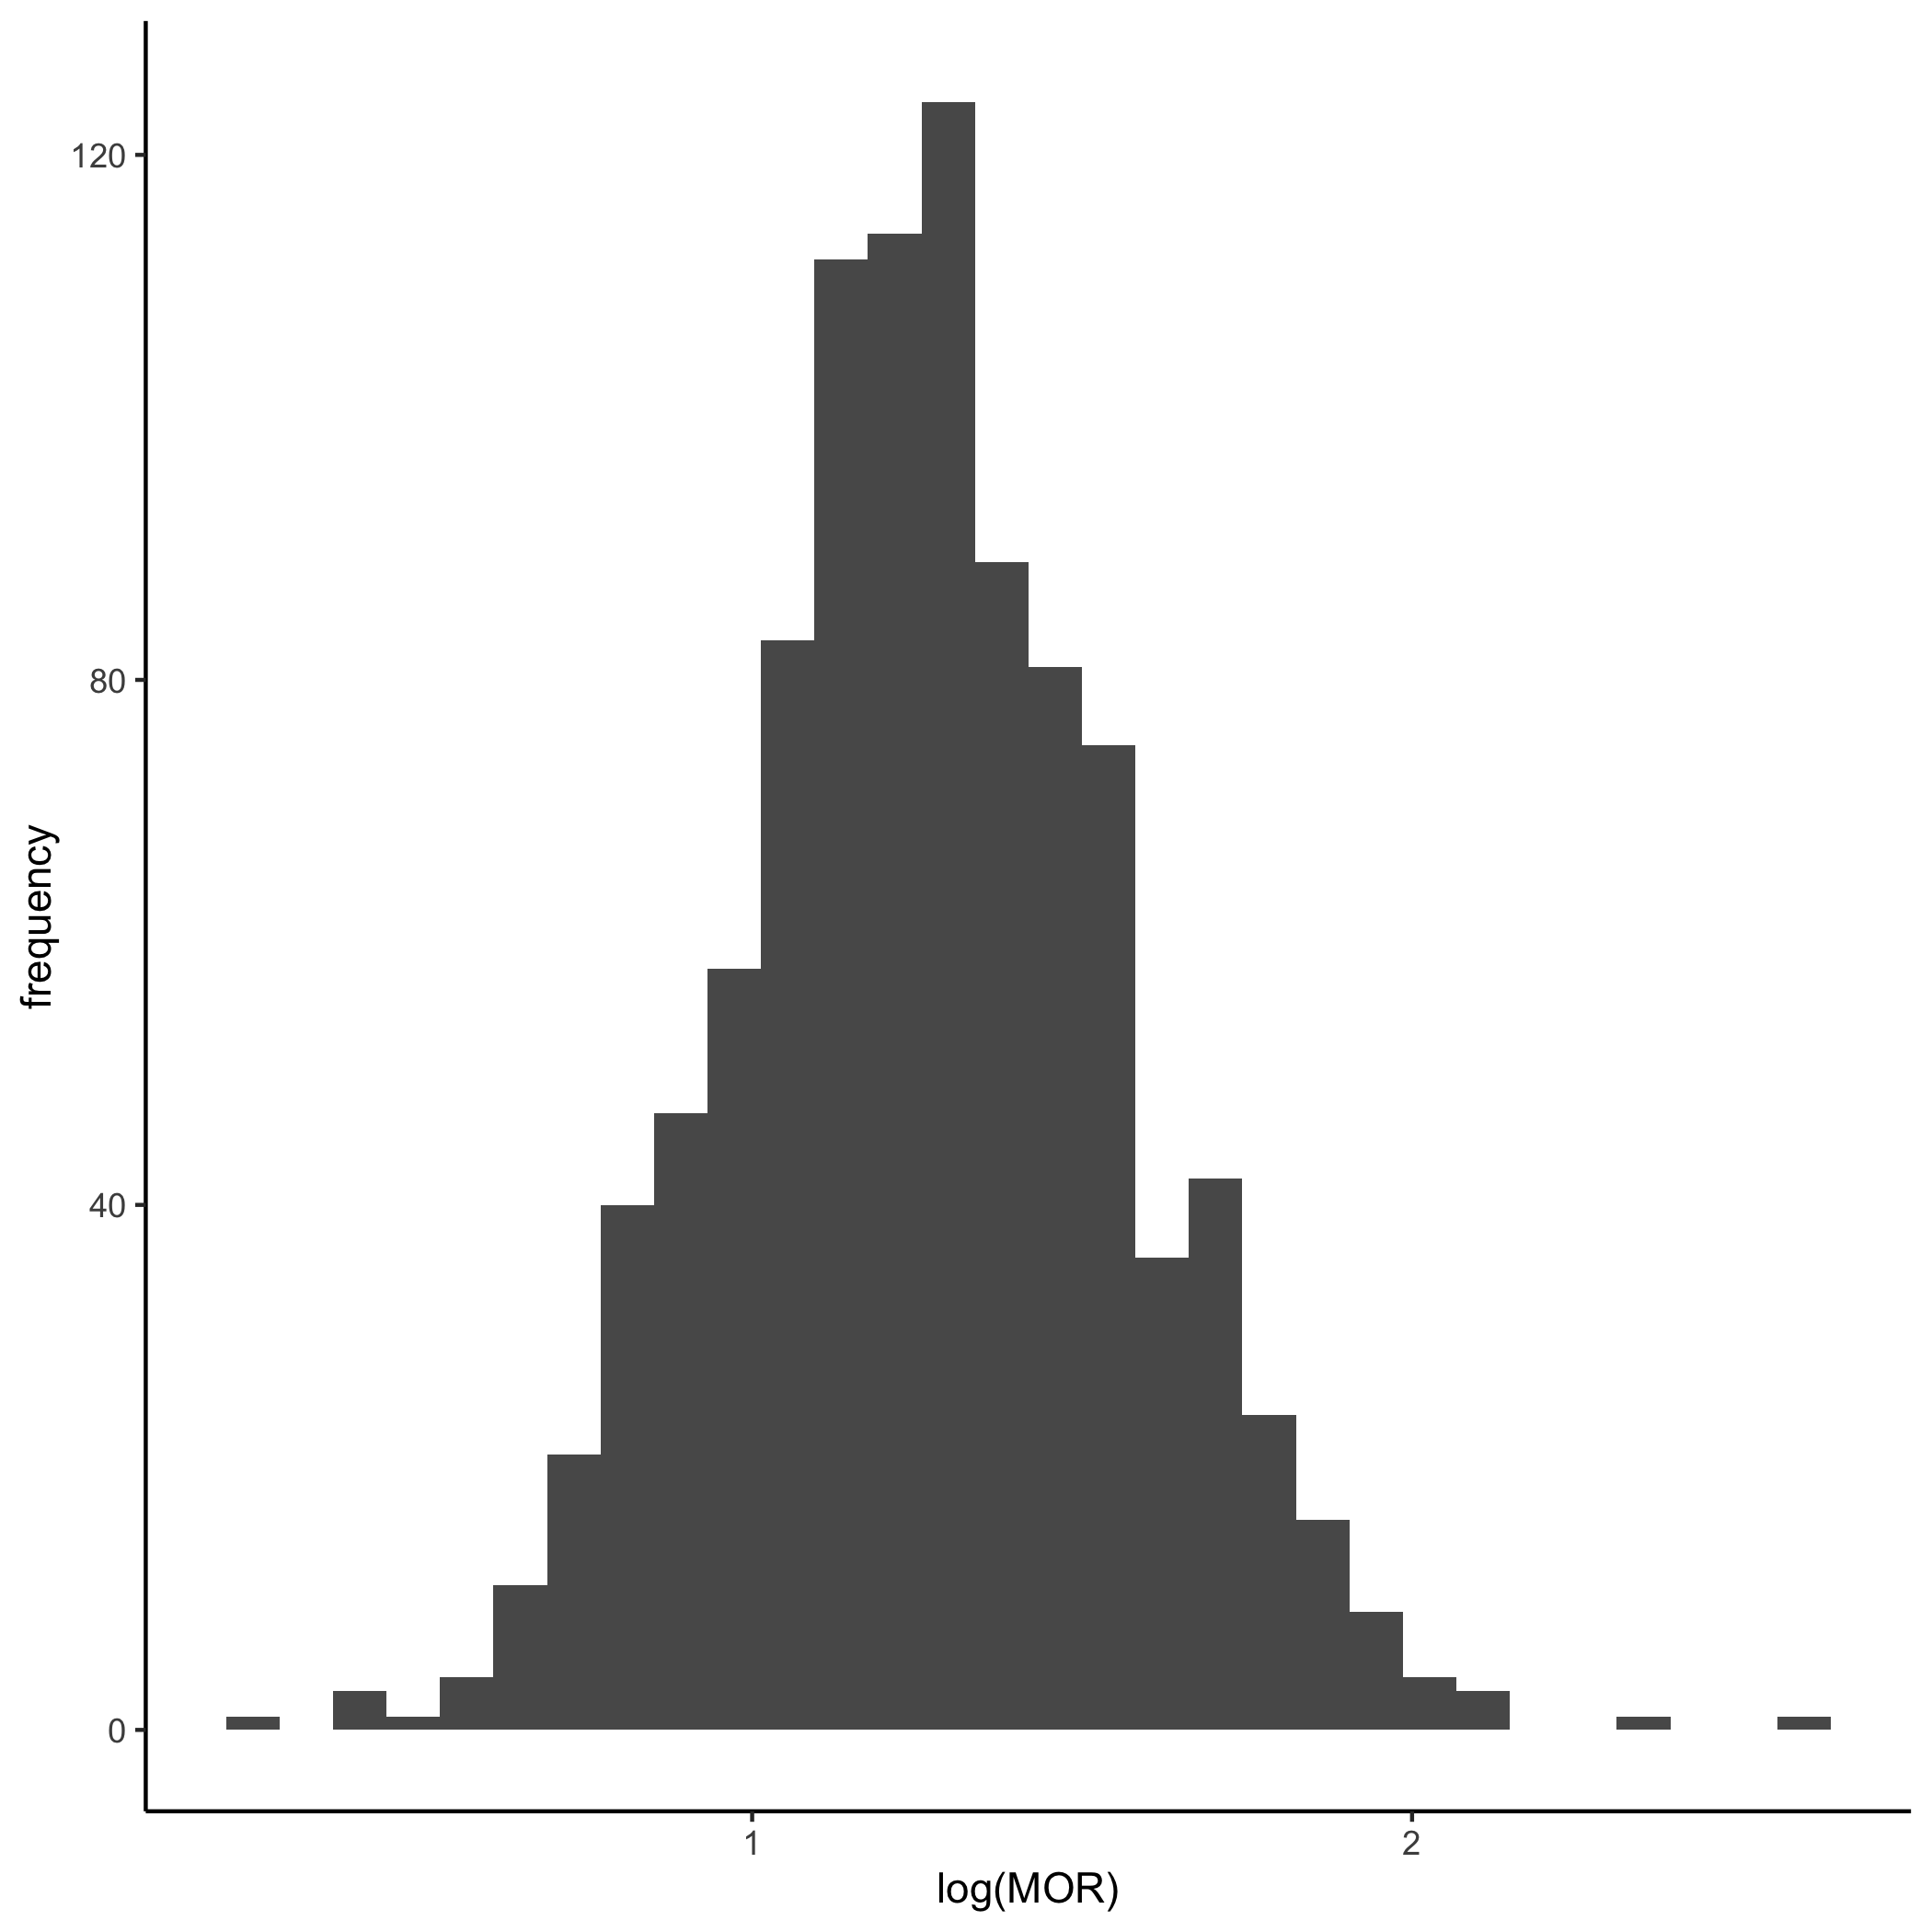
\includegraphics{../../plots/two-lvl-ran-slope/high-prev/hist_30_30_two_lvl_slp_high_prev_q1.png}

}

\caption{Cluster size 30}

}

\end{minipage}%
%
\begin{minipage}[t]{0.24\linewidth}

{\centering 

\raisebox{-\height}{

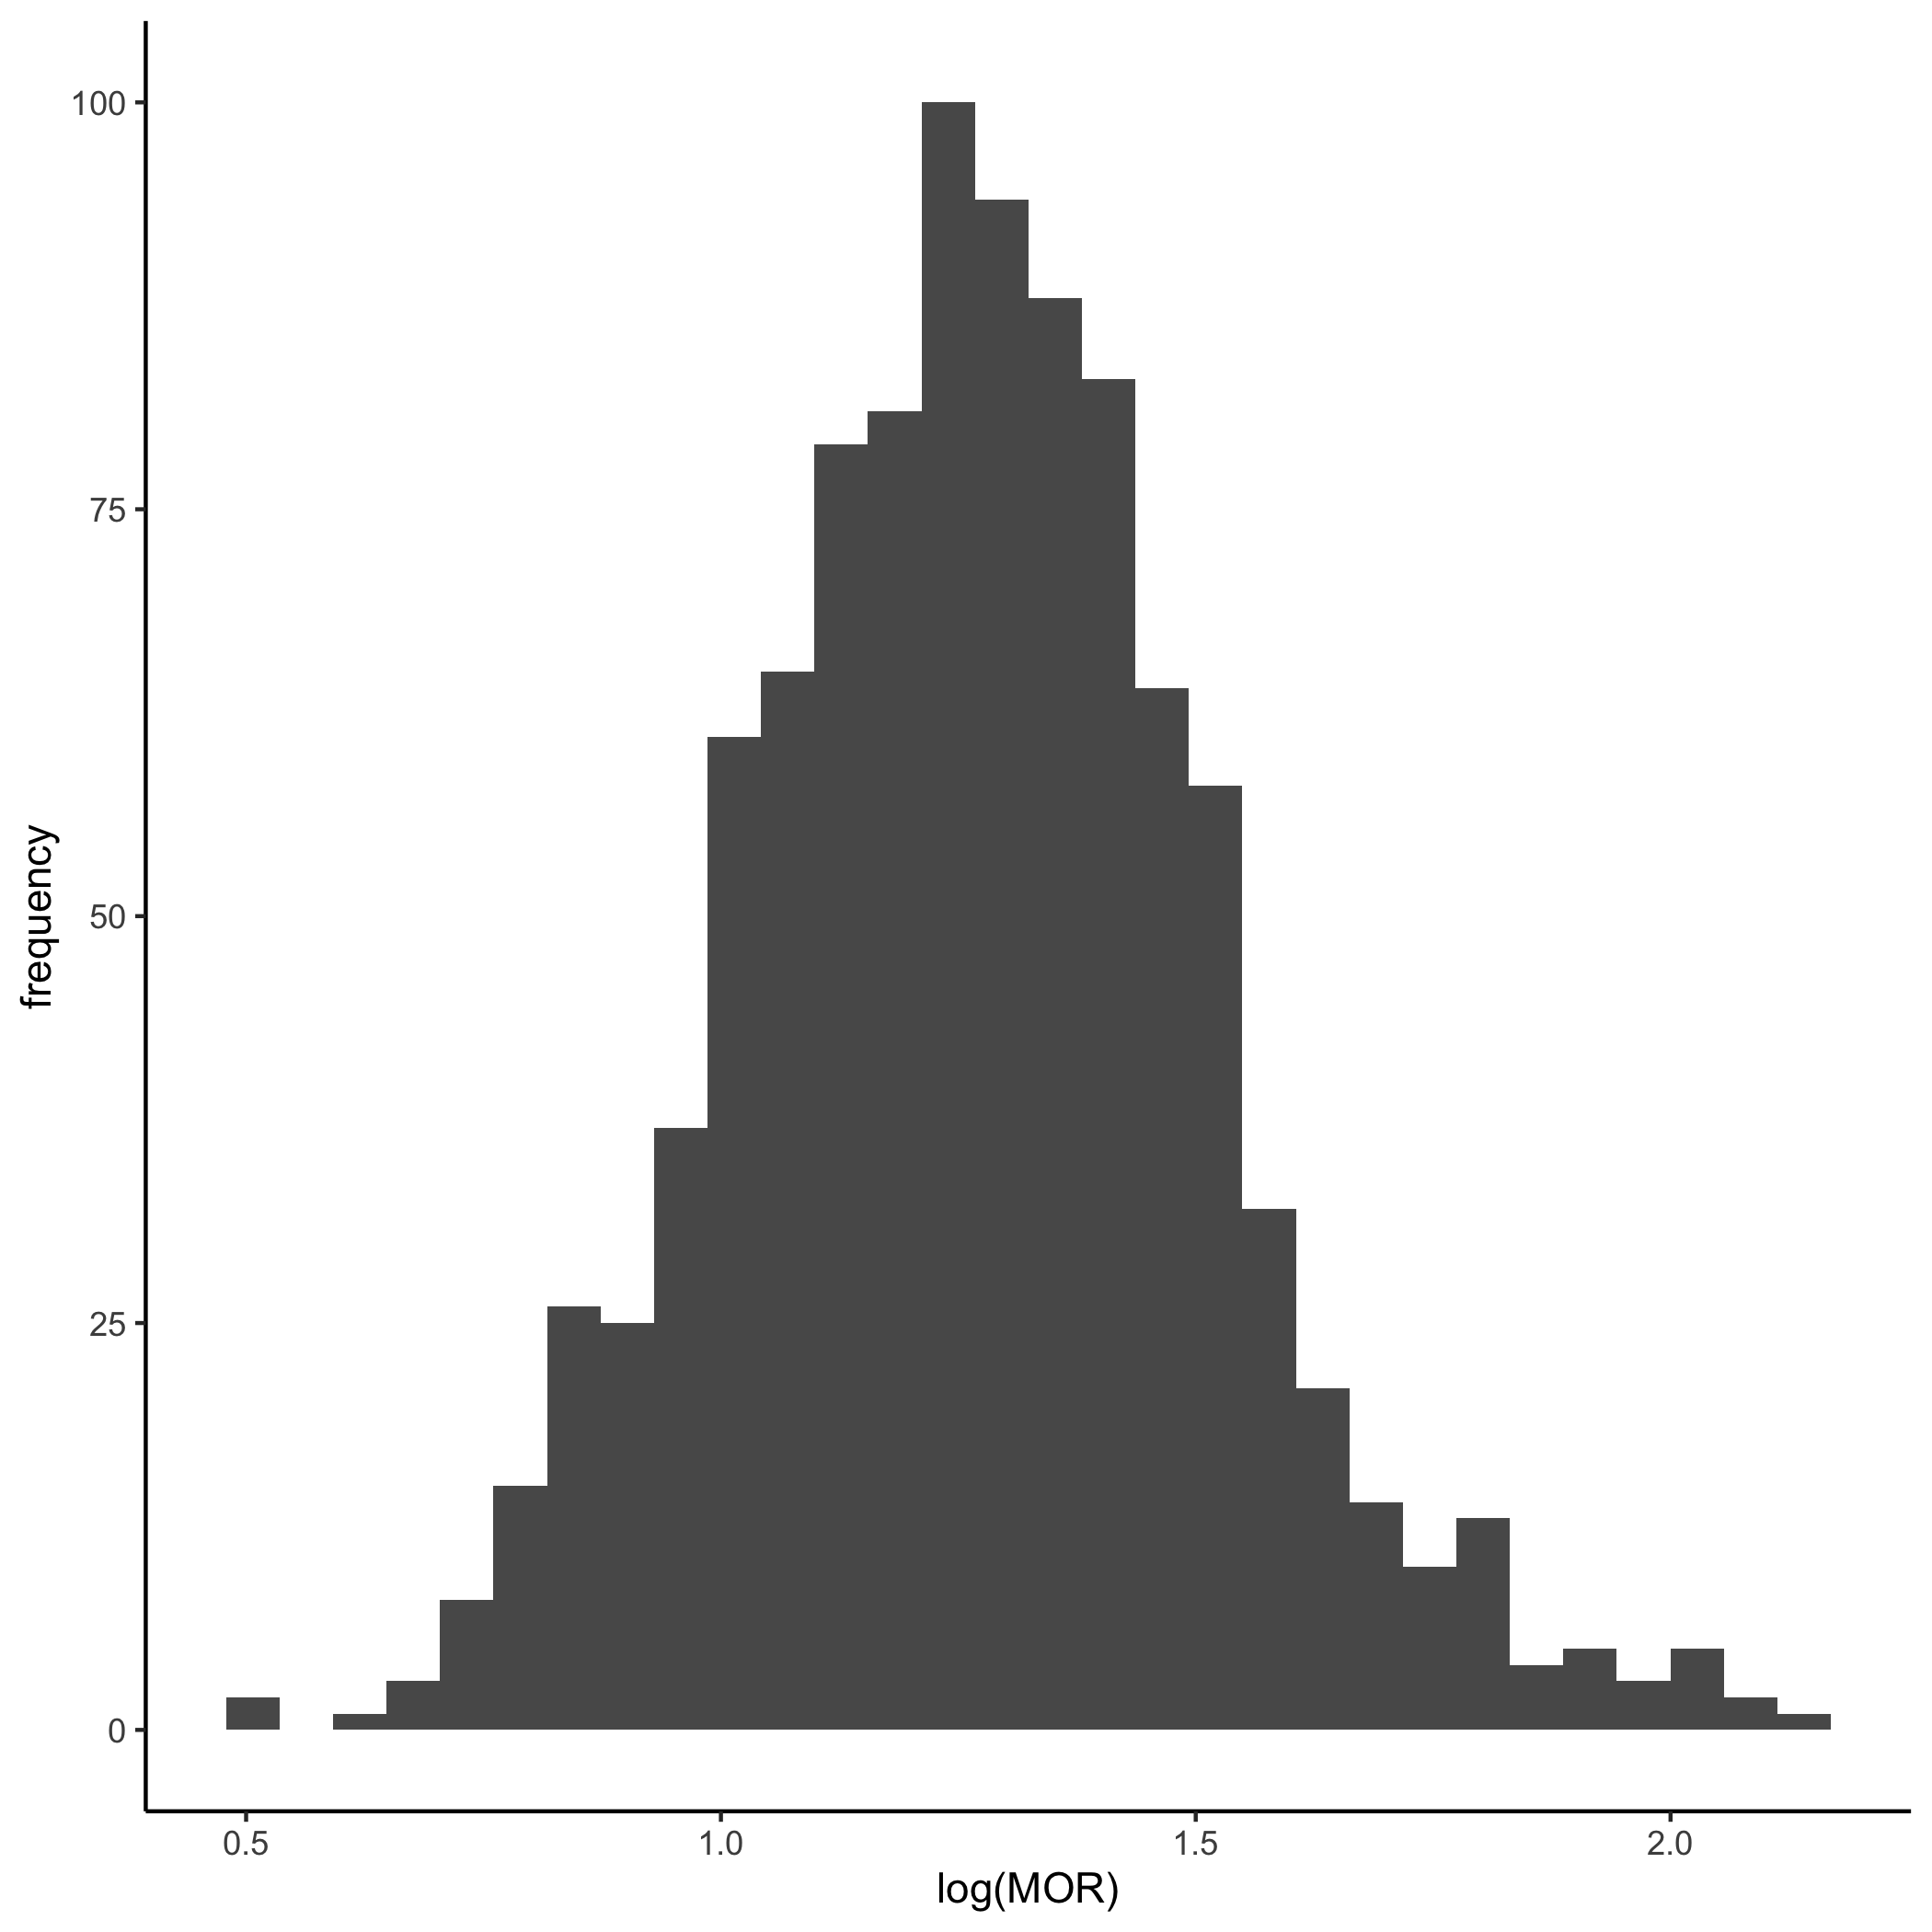
\includegraphics{../../plots/two-lvl-ran-slope/high-prev/hist_30_50_two_lvl_slp_high_prev_q1.png}

}

\caption{Cluster size 50}

}

\end{minipage}%
\newline
\begin{minipage}[t]{\linewidth}

{\centering 

~

}

\end{minipage}%
\newline
\begin{minipage}[t]{0.05\linewidth}

{\centering 

\rotatebox[origin=br]{90}{\tiny Cluster Number 50}

}

\end{minipage}%
%
\begin{minipage}[t]{0.24\linewidth}

{\centering 

\raisebox{-\height}{

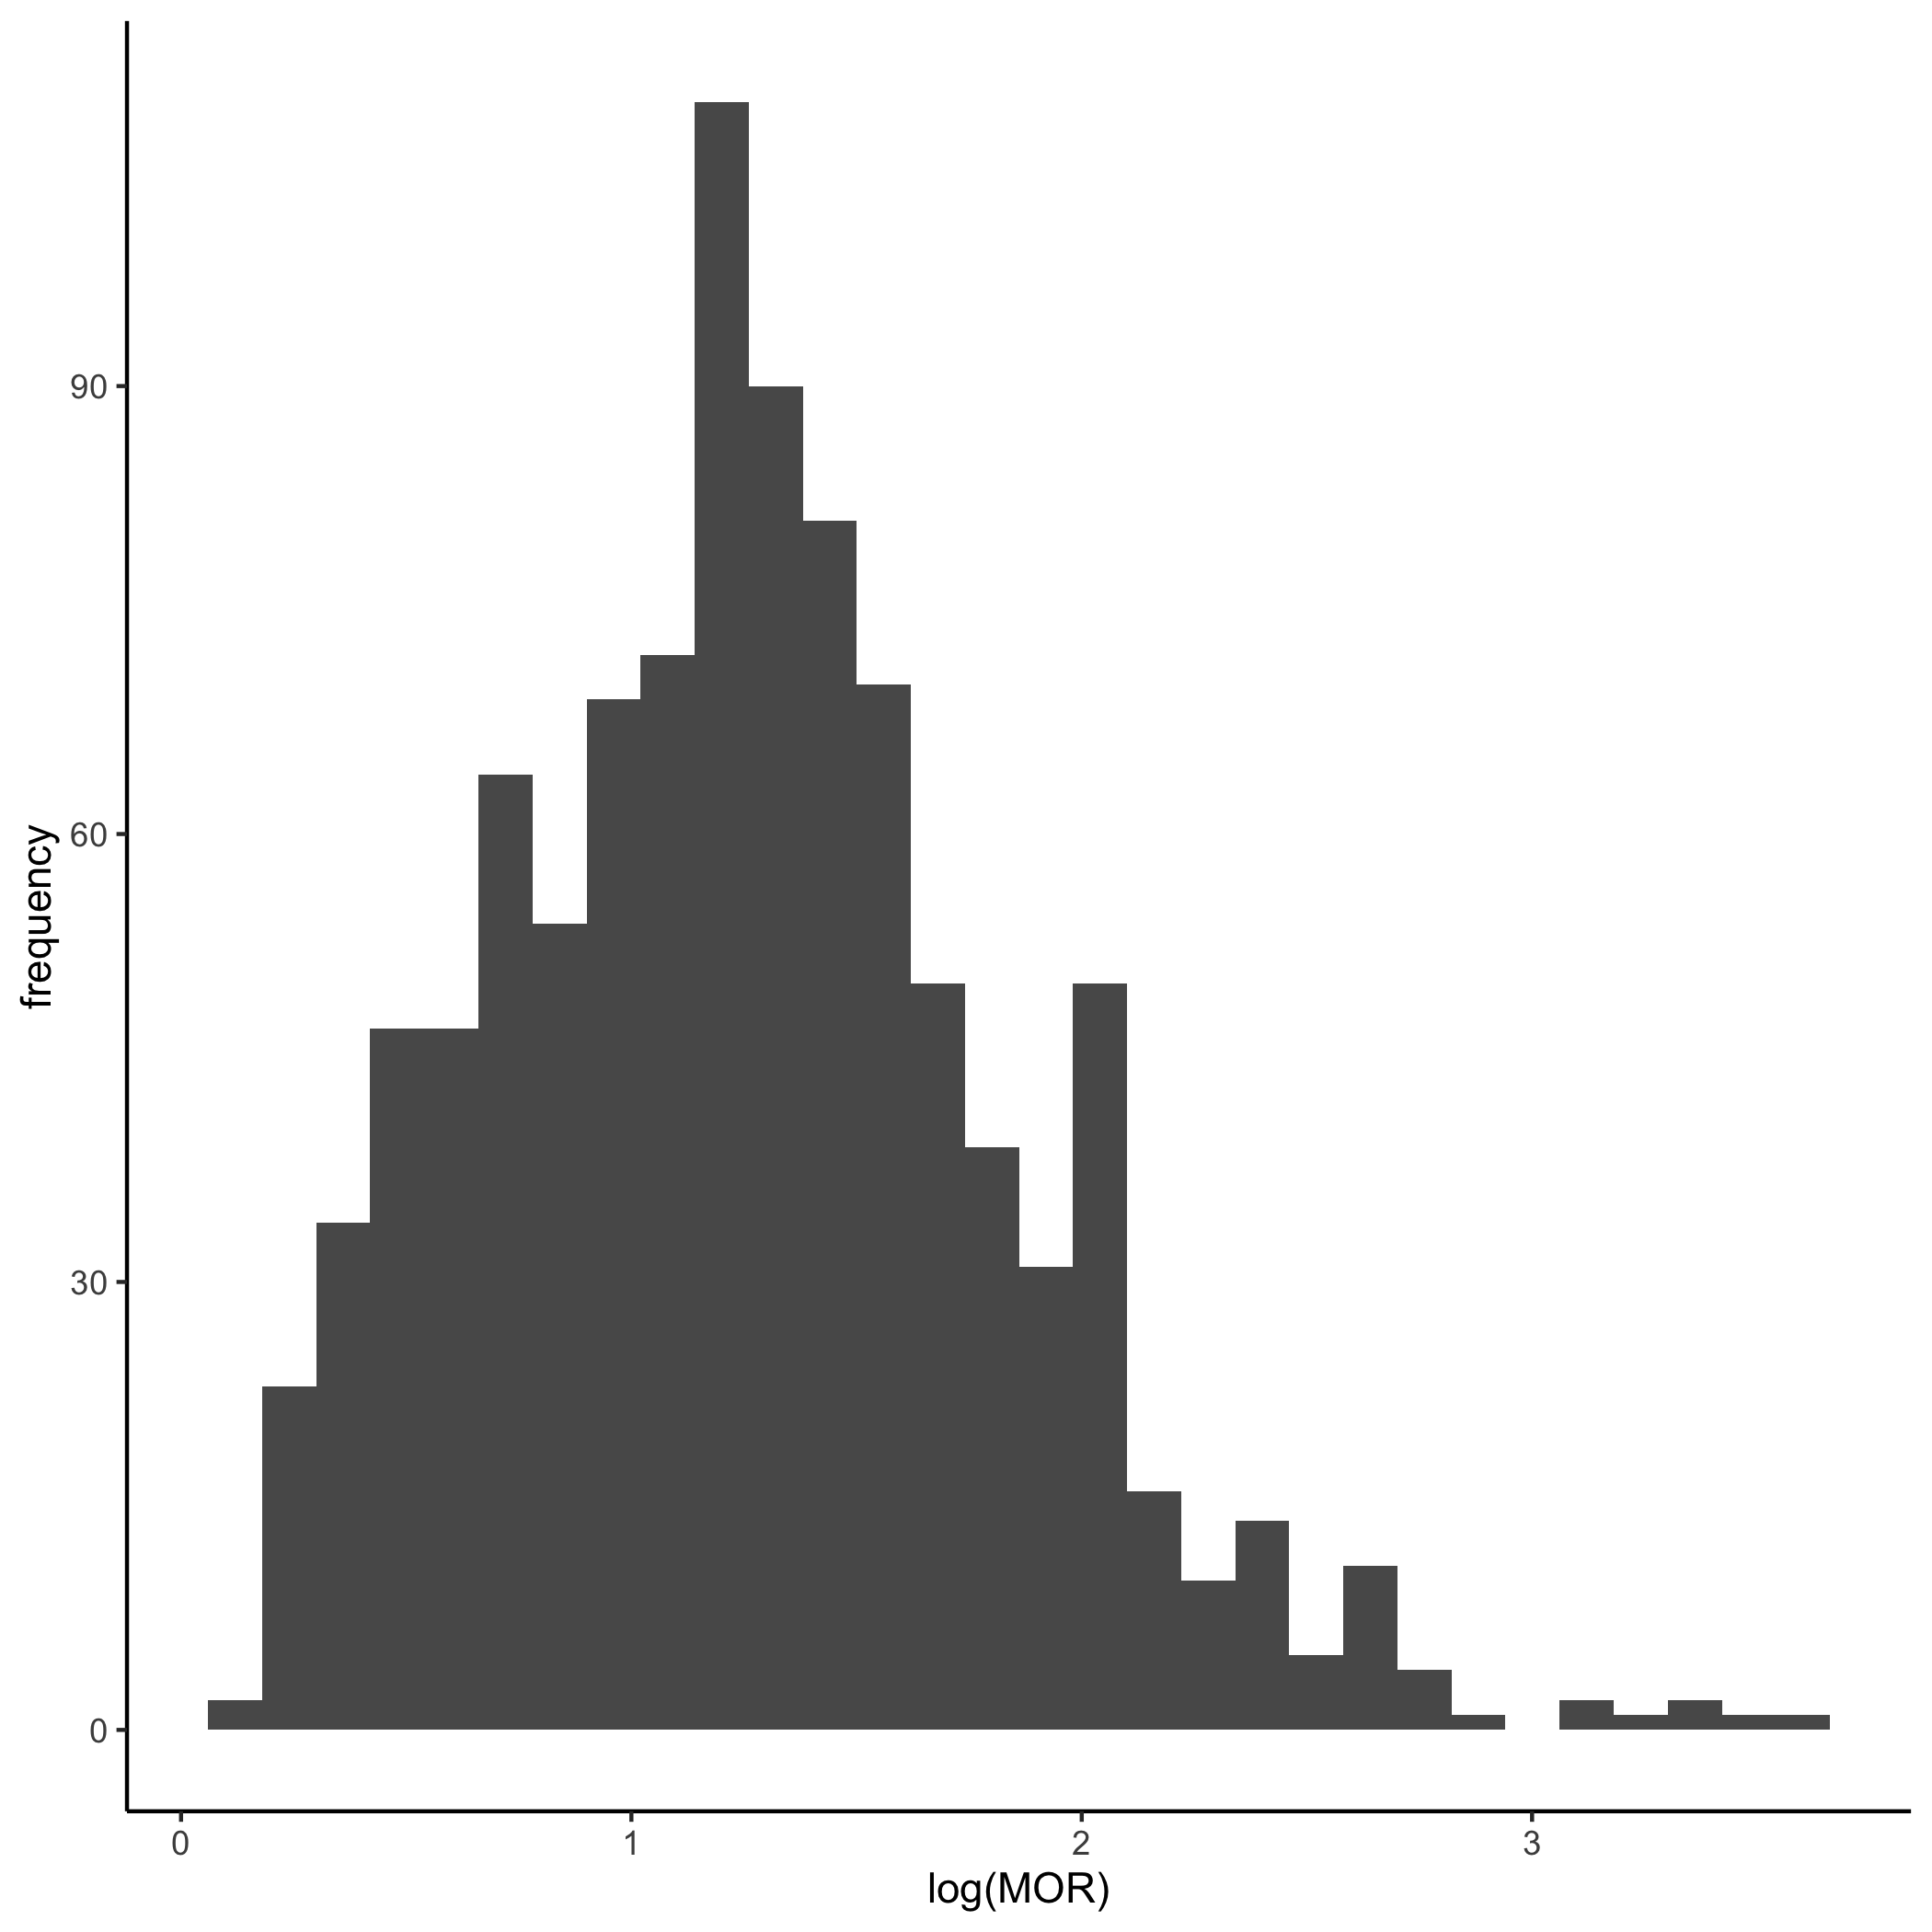
\includegraphics{../../plots/two-lvl-ran-slope/high-prev/hist_50_5_two_lvl_slp_high_prev_q1.png}

}

\caption{Cluster size 5}

}

\end{minipage}%
%
\begin{minipage}[t]{0.24\linewidth}

{\centering 

\raisebox{-\height}{

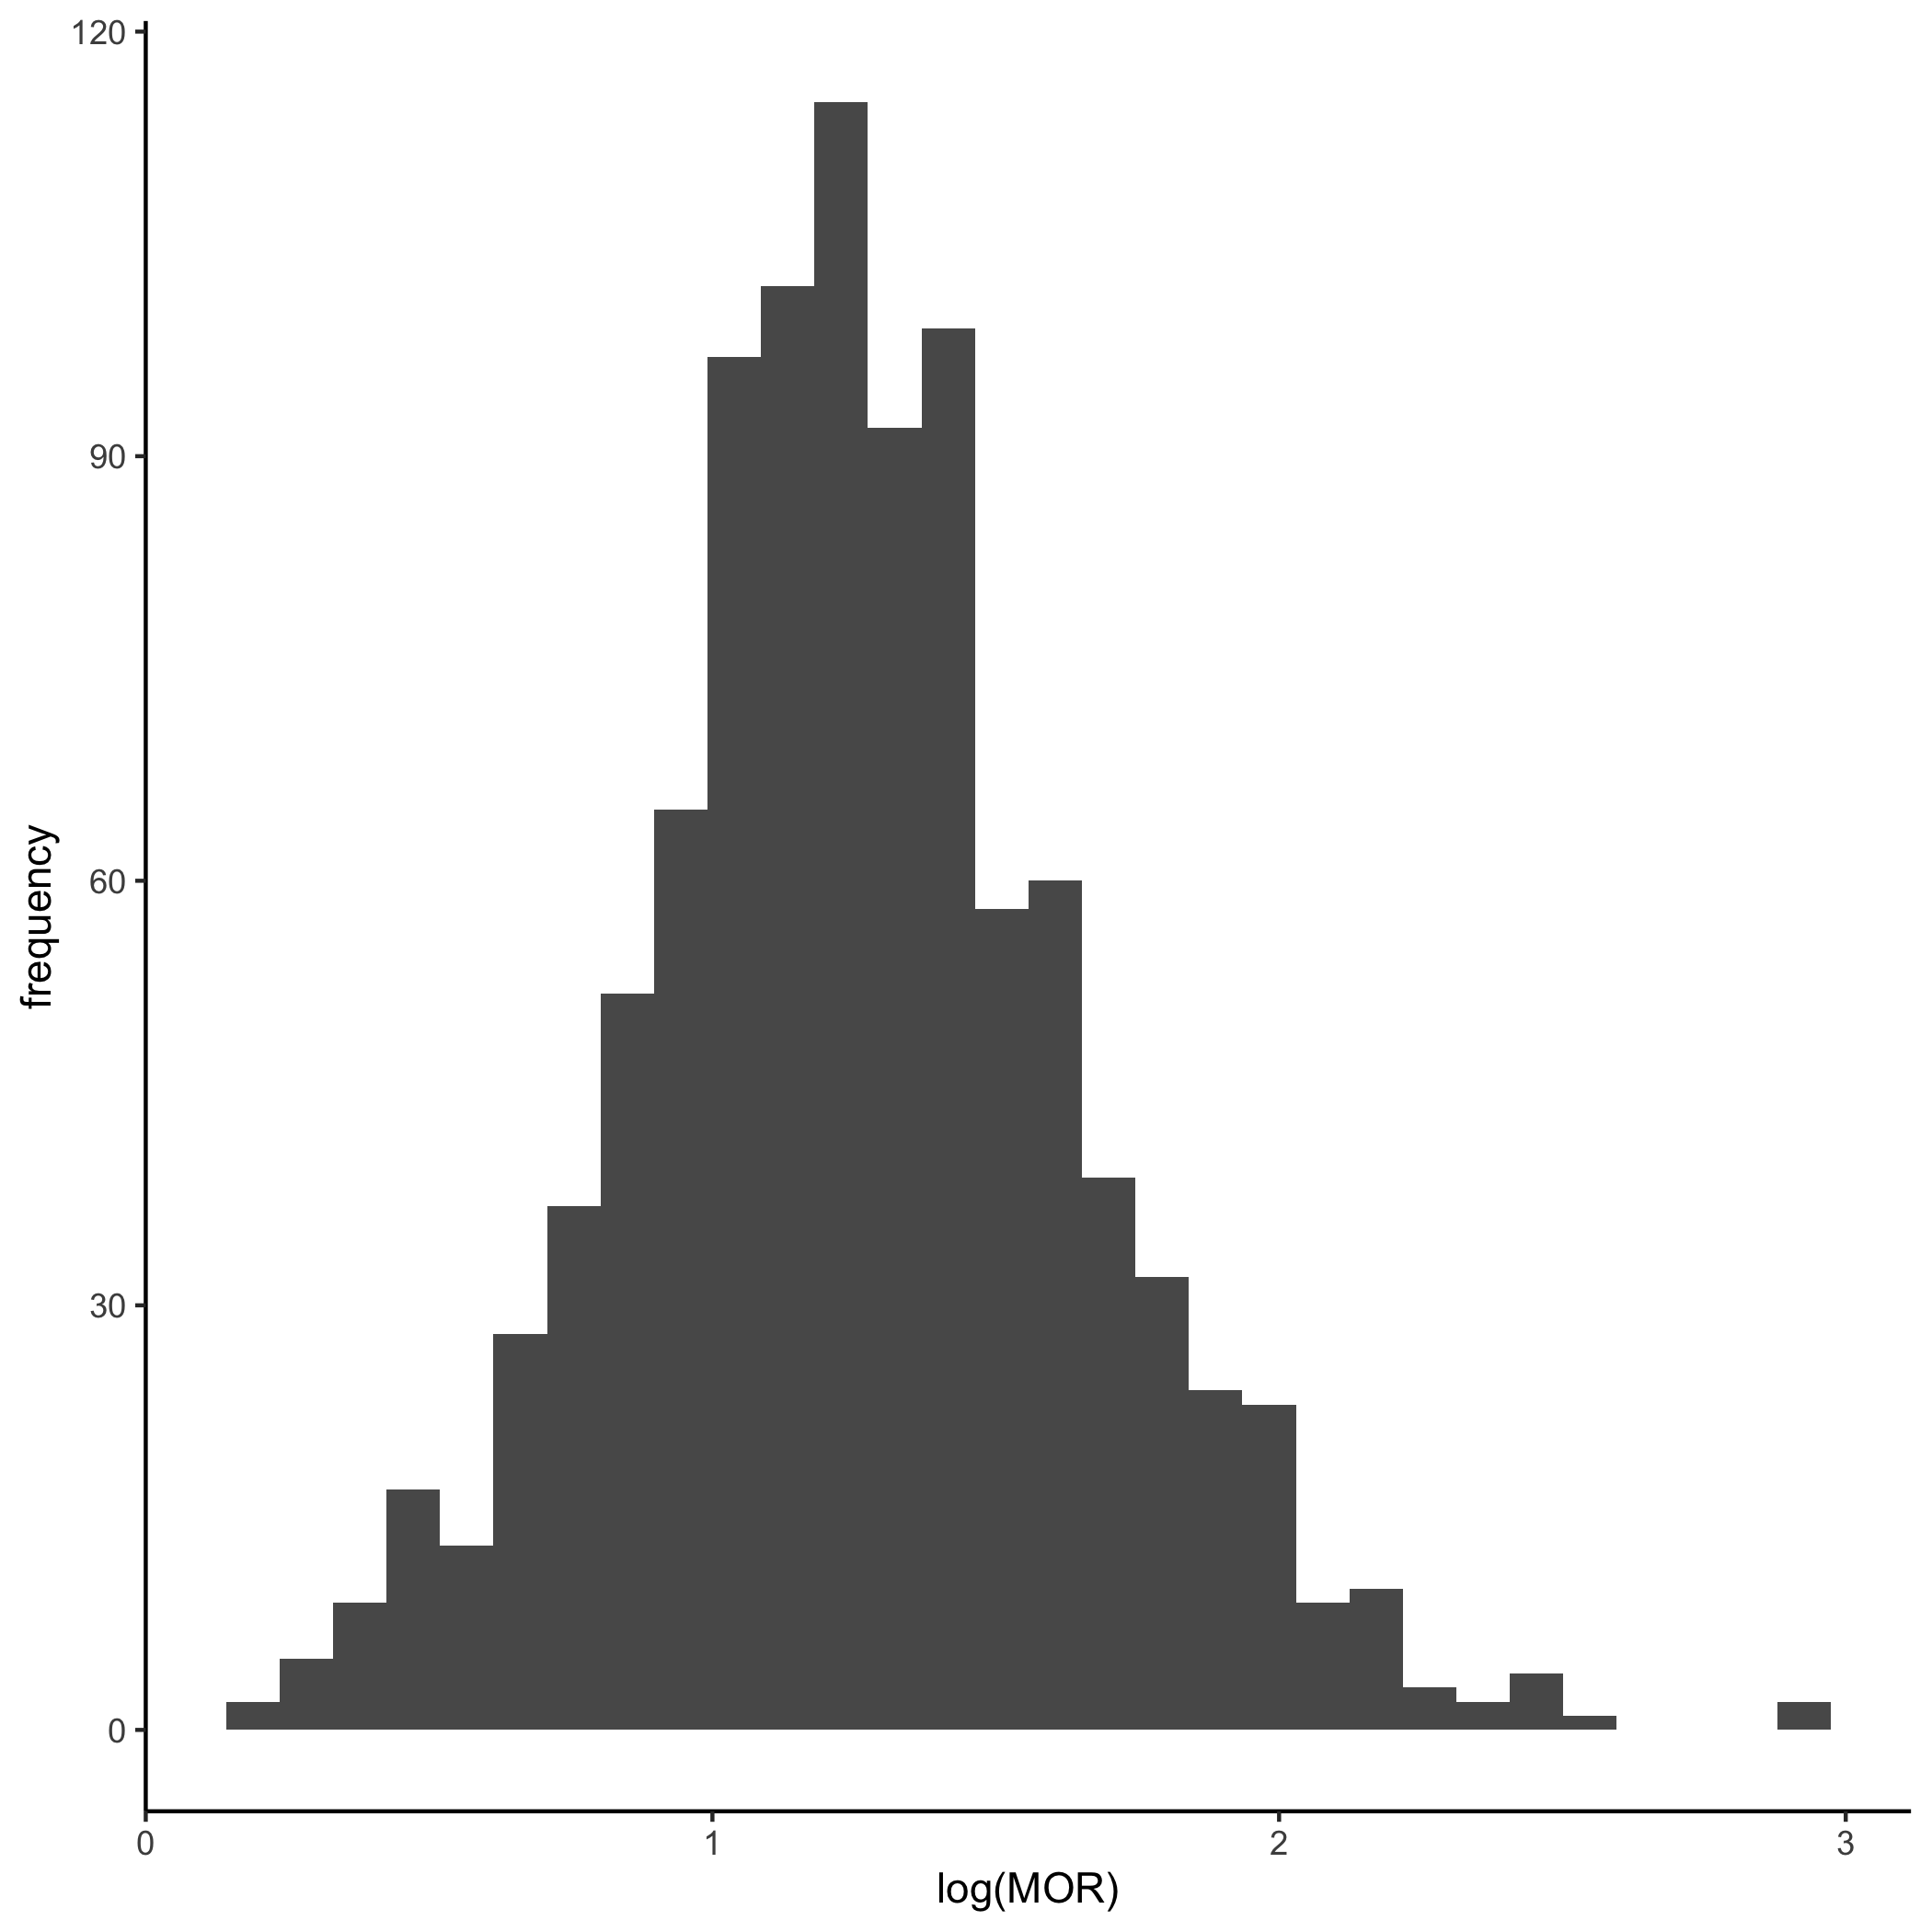
\includegraphics{../../plots/two-lvl-ran-slope/high-prev/hist_50_10_two_lvl_slp_high_prev_q1.png}

}

\caption{Cluster size 10}

}

\end{minipage}%
%
\begin{minipage}[t]{0.24\linewidth}

{\centering 

\raisebox{-\height}{

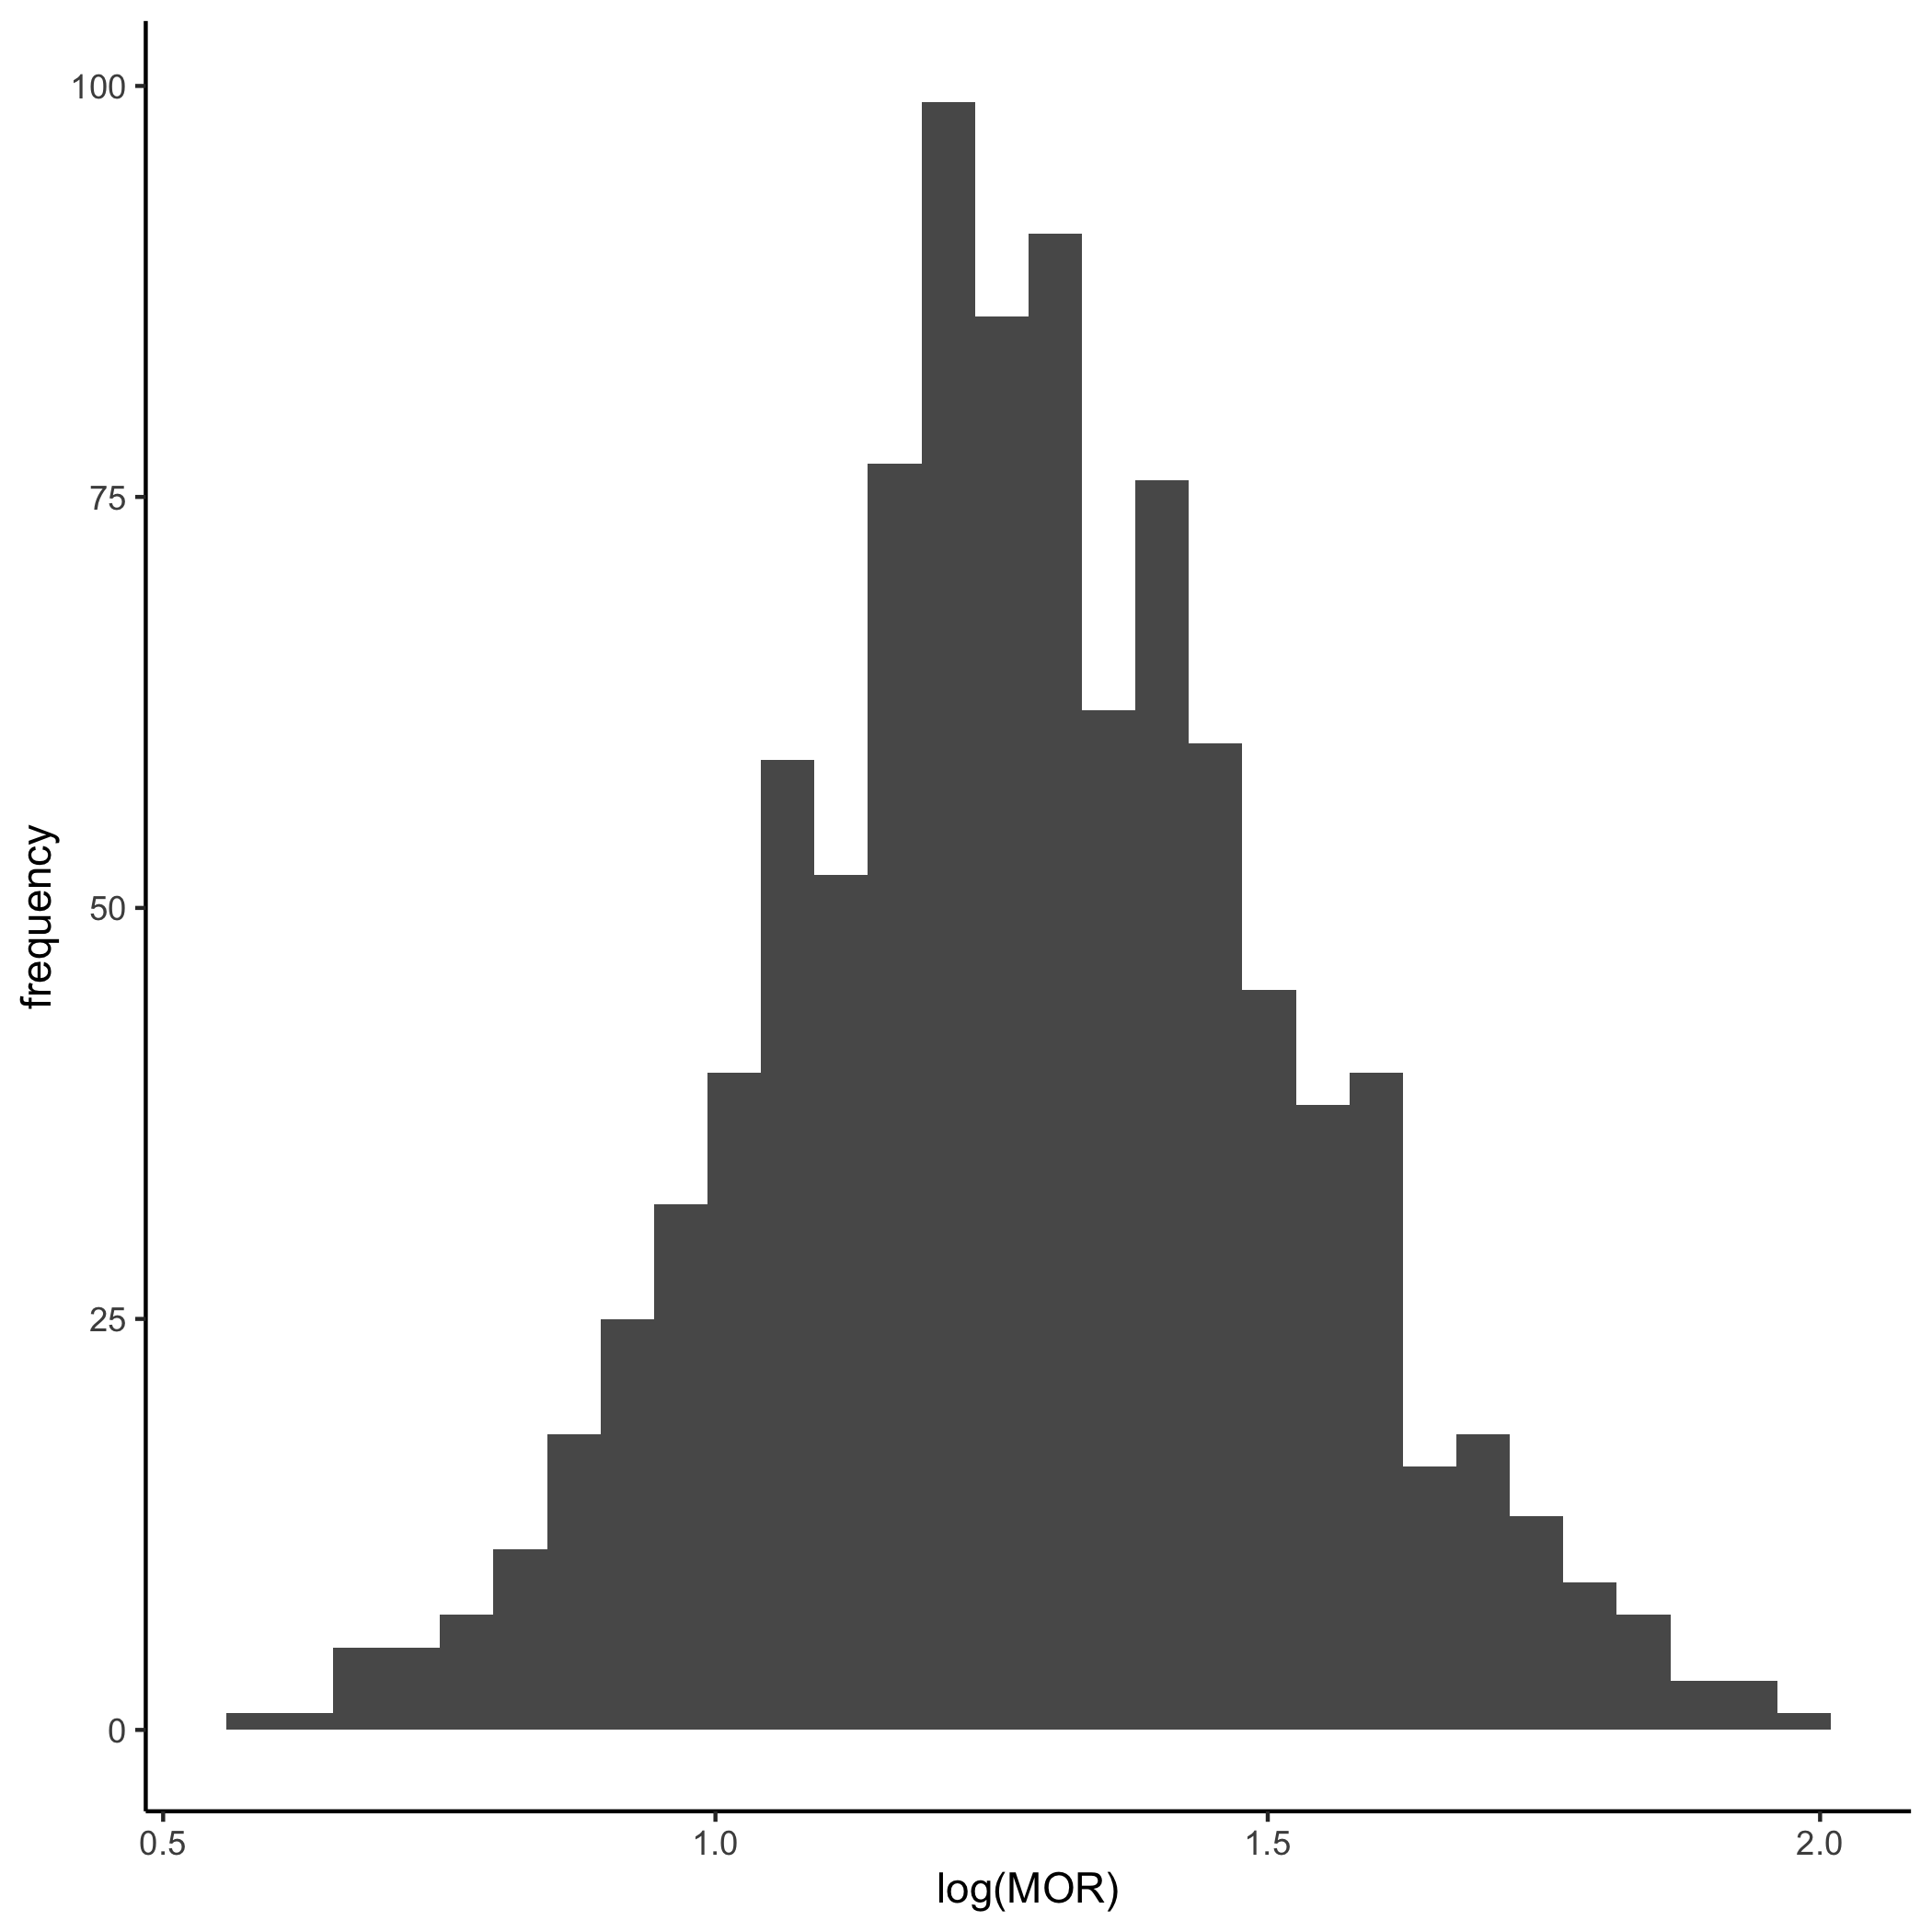
\includegraphics{../../plots/two-lvl-ran-slope/high-prev/hist_50_30_two_lvl_slp_high_prev_q1.png}

}

\caption{Cluster size 30}

}

\end{minipage}%
%
\begin{minipage}[t]{0.24\linewidth}

{\centering 

\raisebox{-\height}{

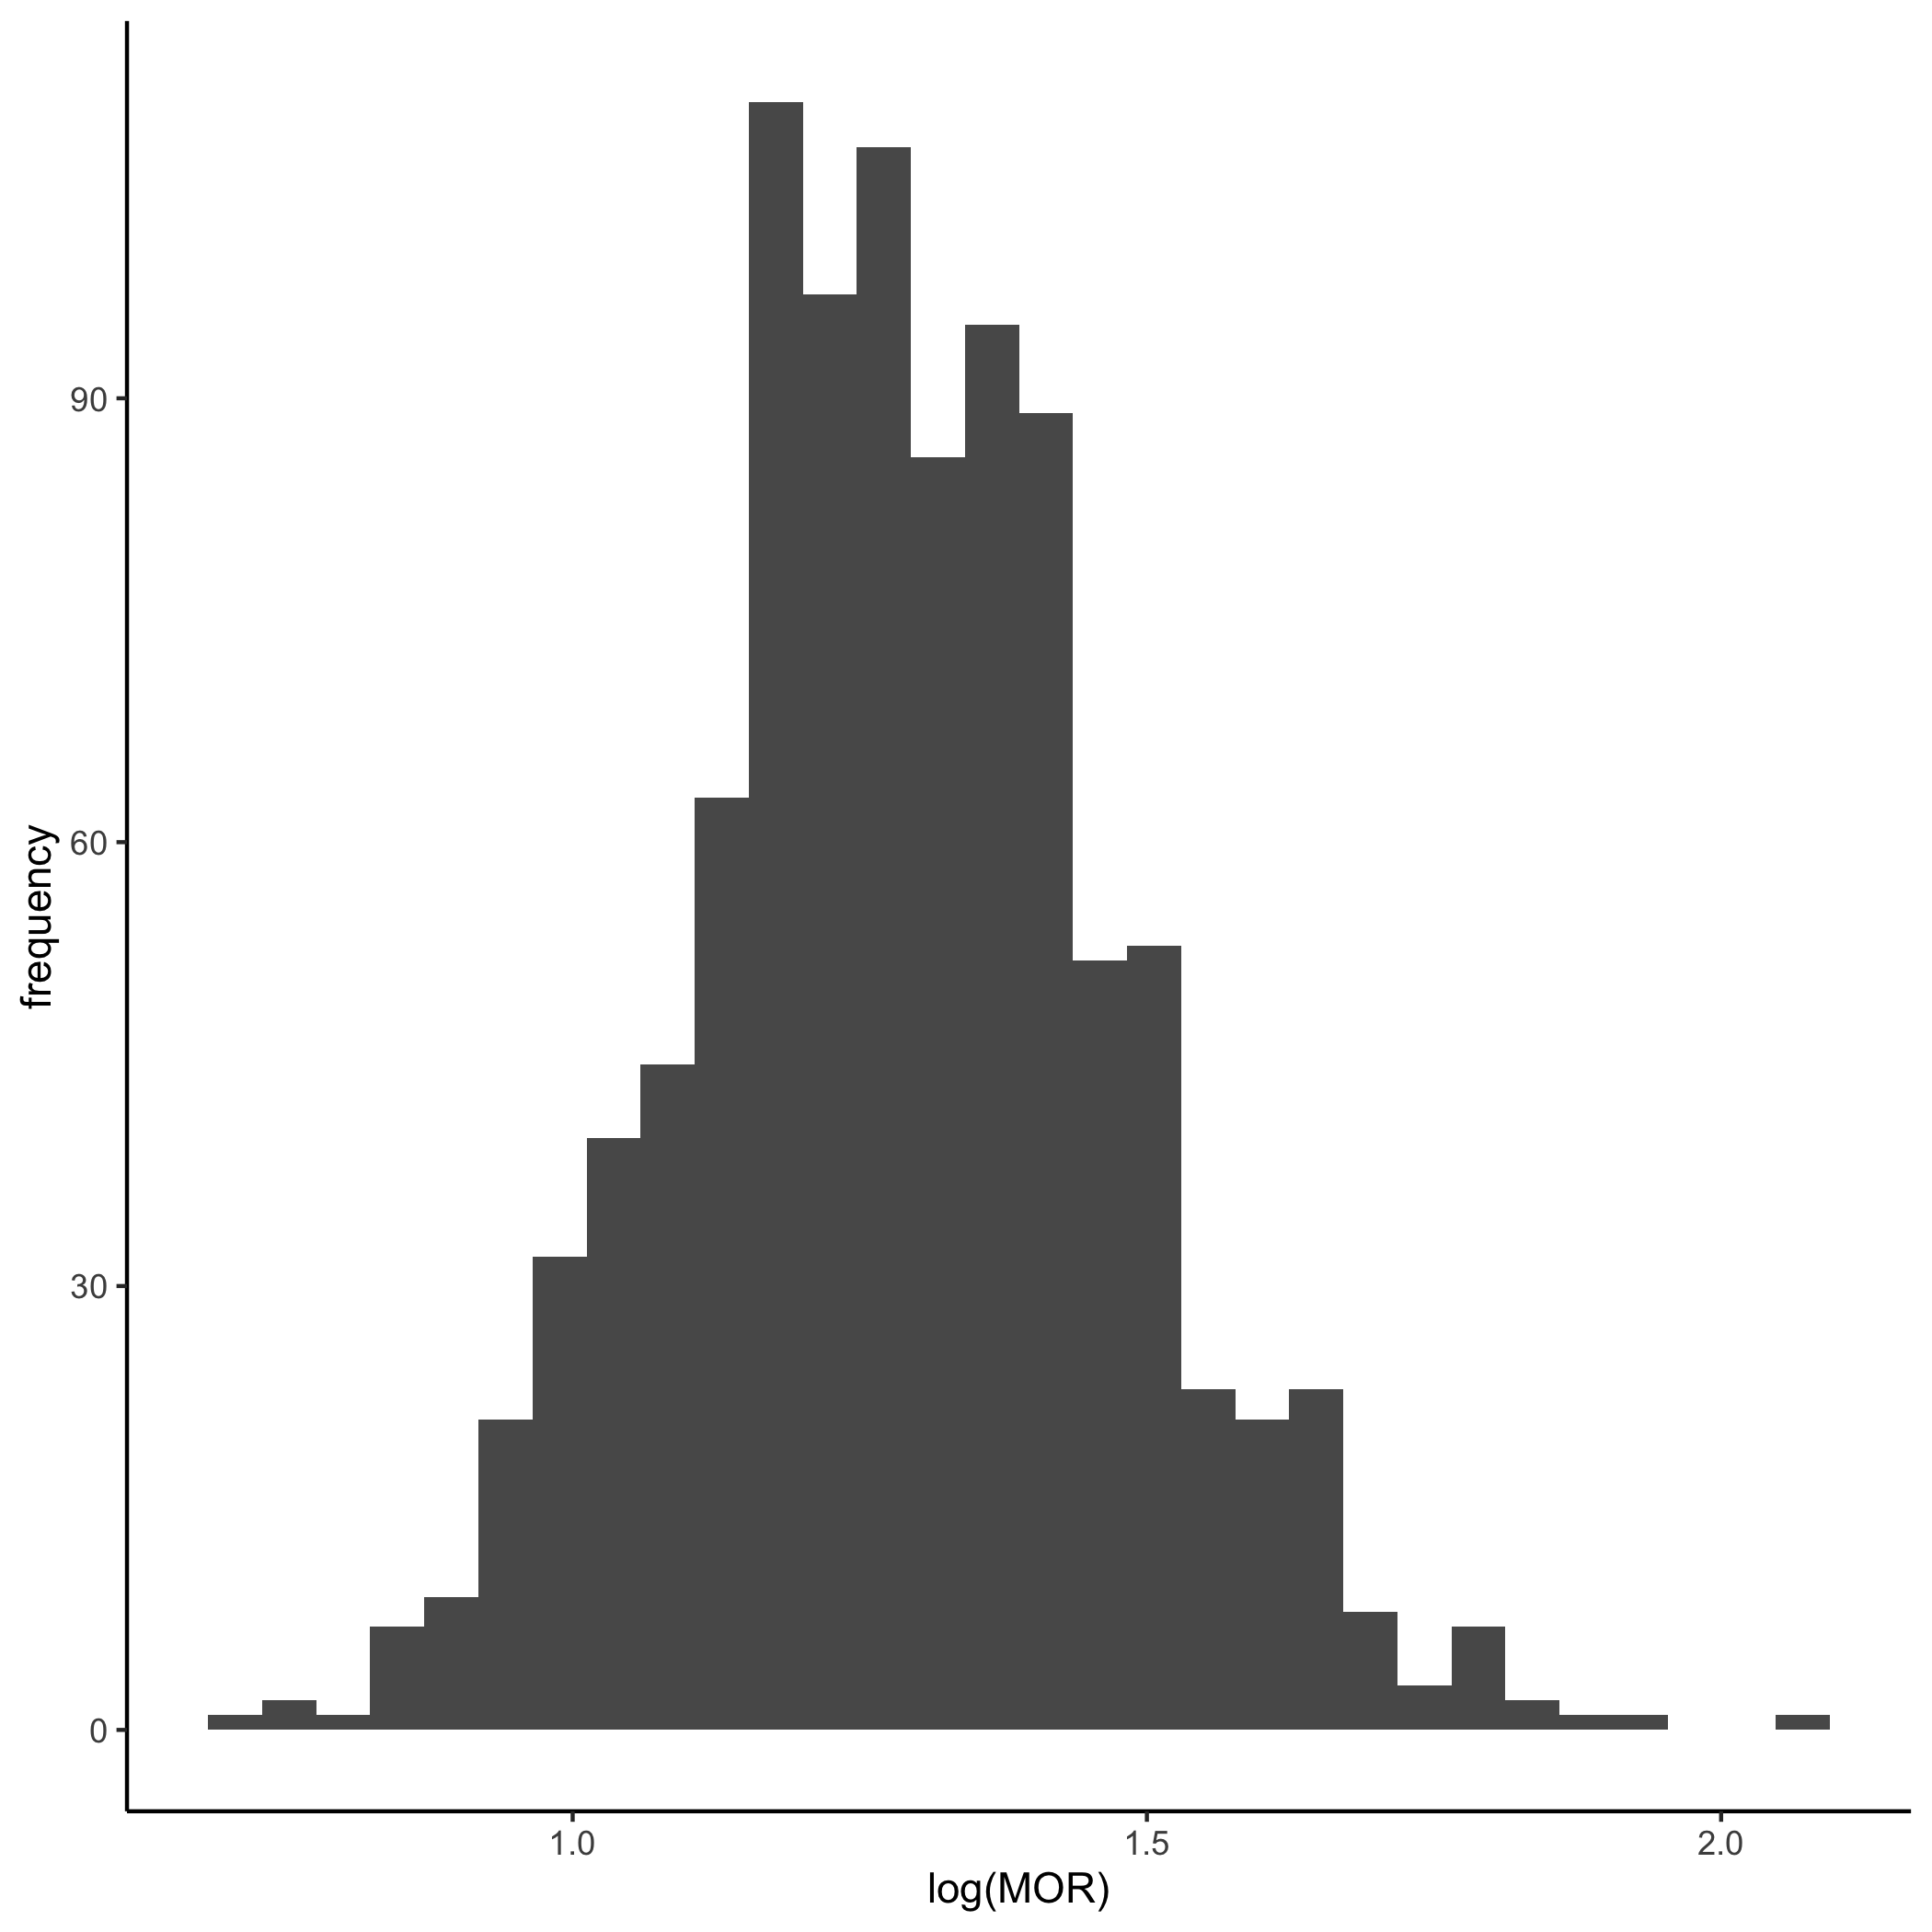
\includegraphics{../../plots/two-lvl-ran-slope/high-prev/hist_50_50_two_lvl_slp_high_prev_q1.png}

}

\caption{Cluster size 50}

}

\end{minipage}%
\newline
\begin{minipage}[t]{\linewidth}

{\centering 

~

}

\end{minipage}%
\newline
\begin{minipage}[t]{0.05\linewidth}

{\centering 

\rotatebox[origin=br]{90}{\tiny Cluster Number 100}

}

\end{minipage}%
%
\begin{minipage}[t]{0.24\linewidth}

{\centering 

\raisebox{-\height}{

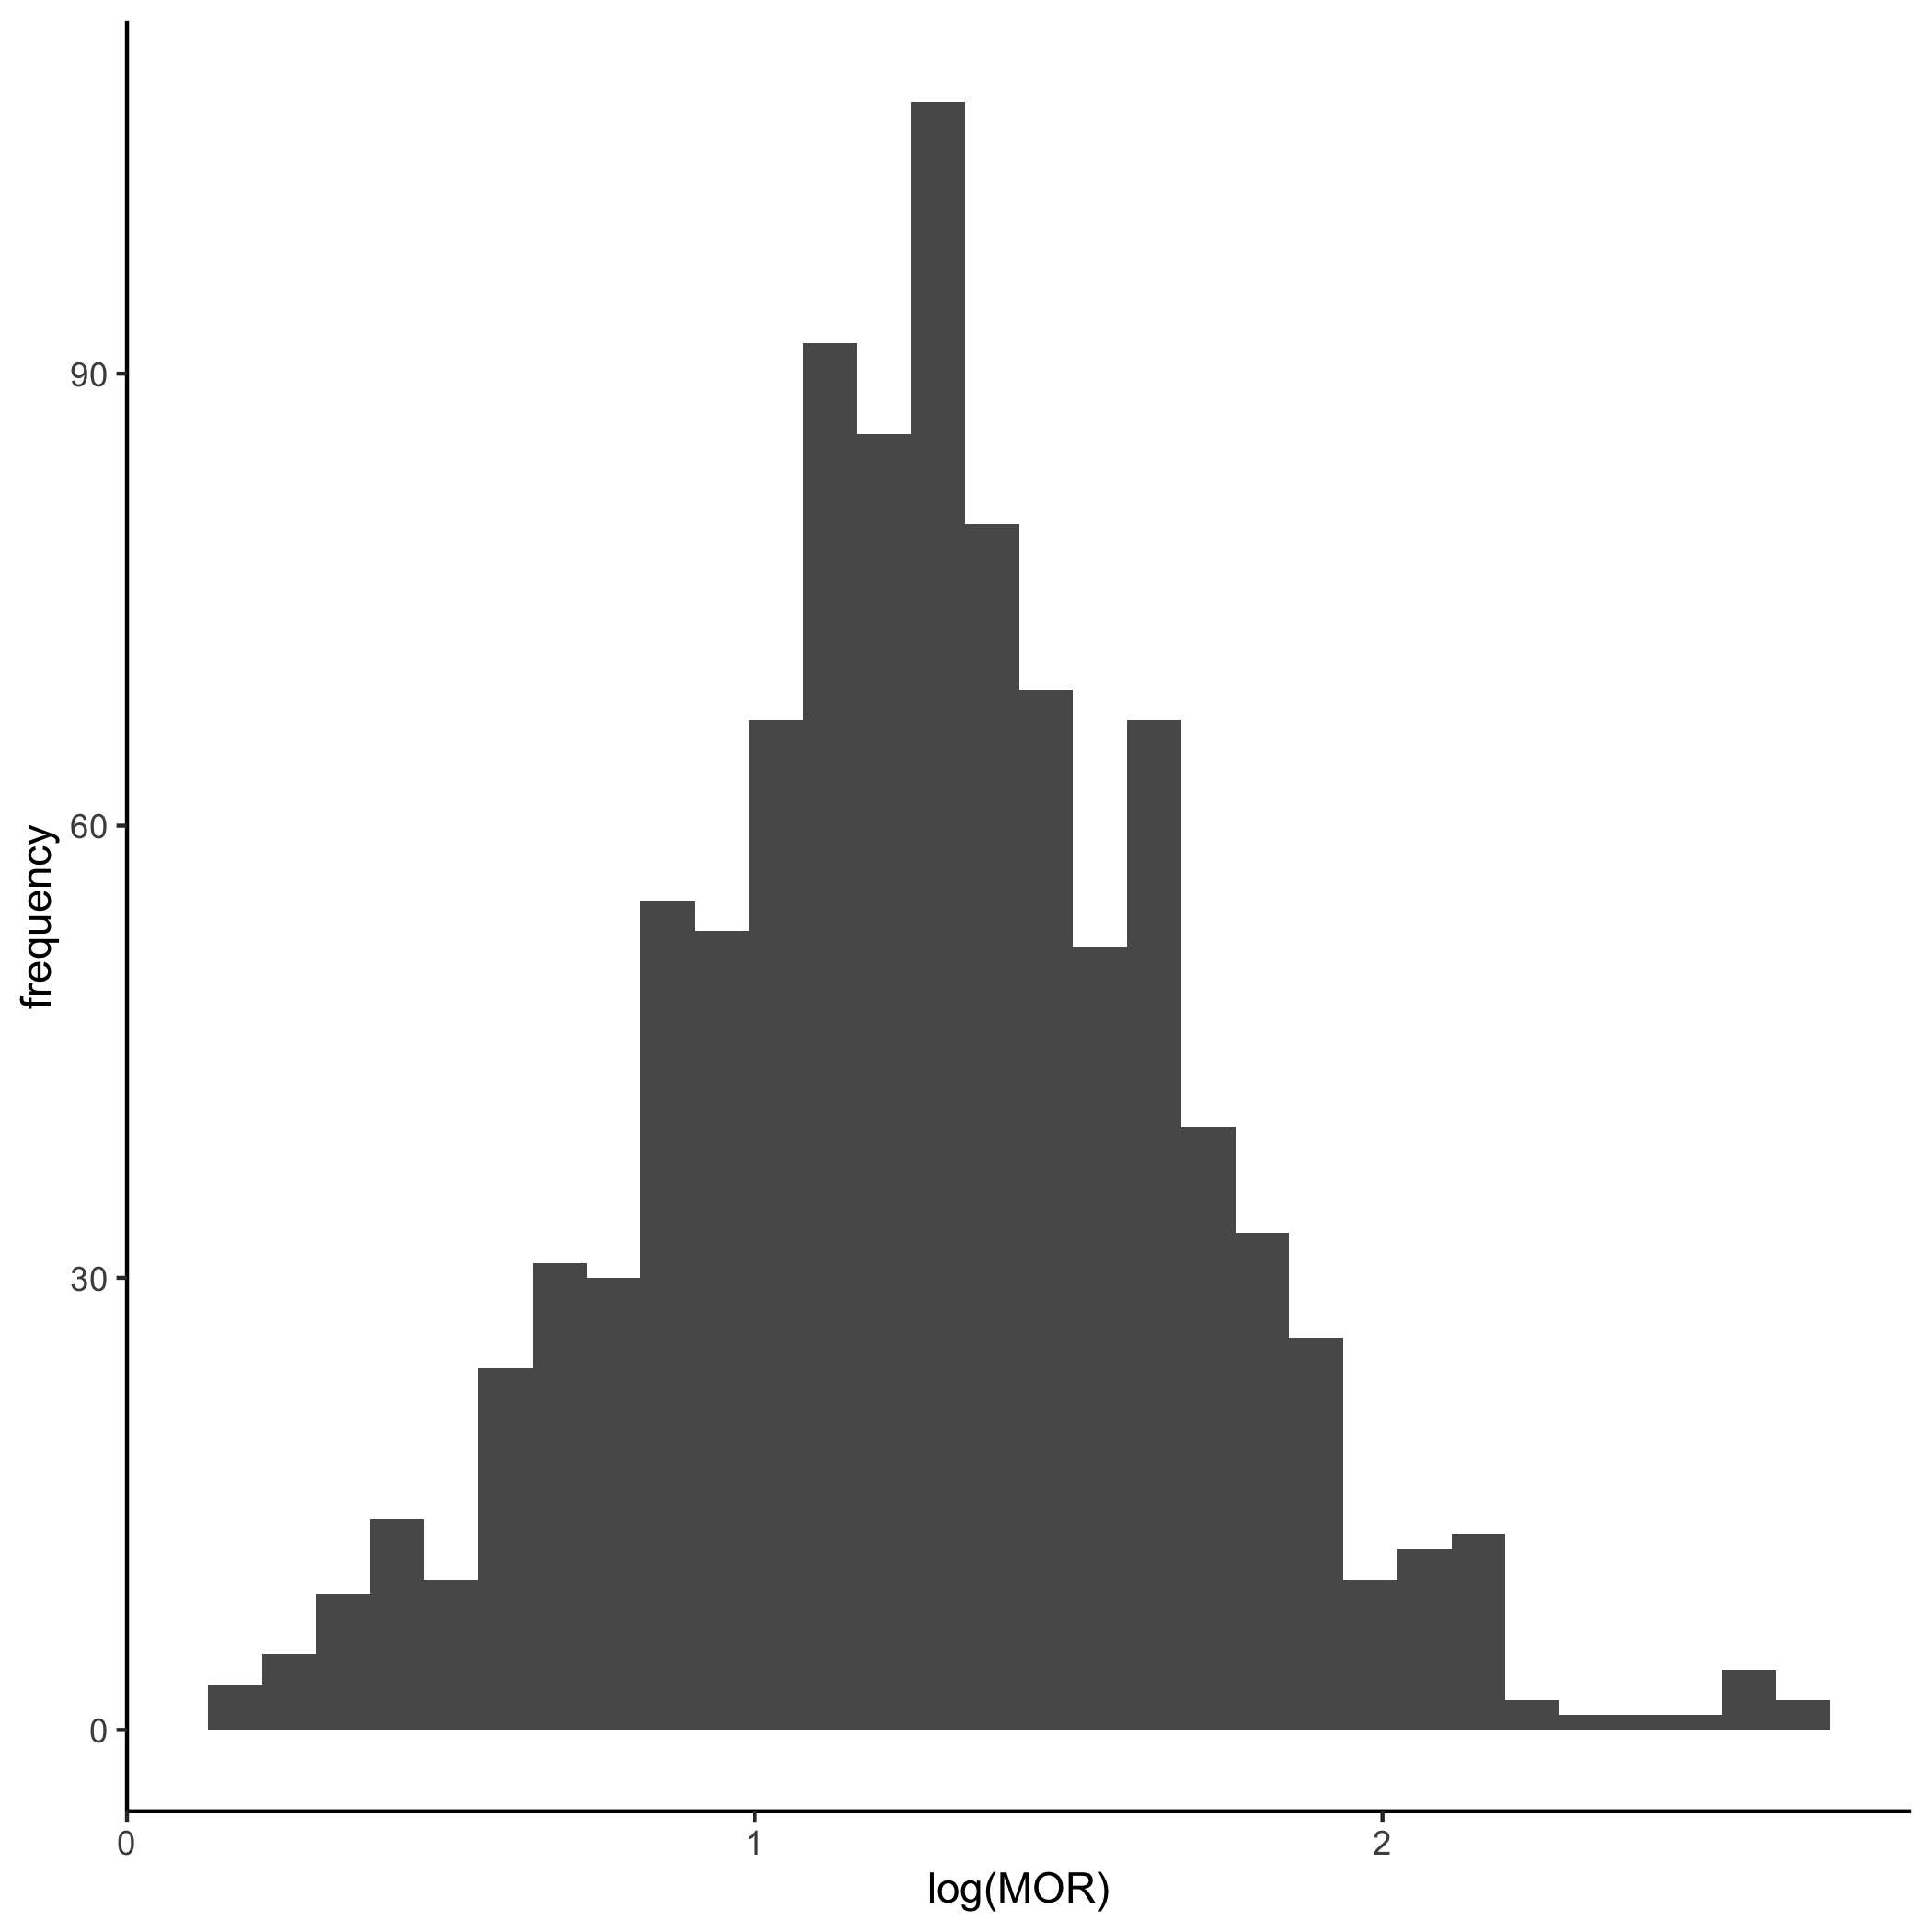
\includegraphics{../../plots/two-lvl-ran-slope/high-prev/hist_100_5_two_lvl_slp_high_prev_q1.png}

}

\caption{Cluster size 5}

}

\end{minipage}%
%
\begin{minipage}[t]{0.24\linewidth}

{\centering 

\raisebox{-\height}{

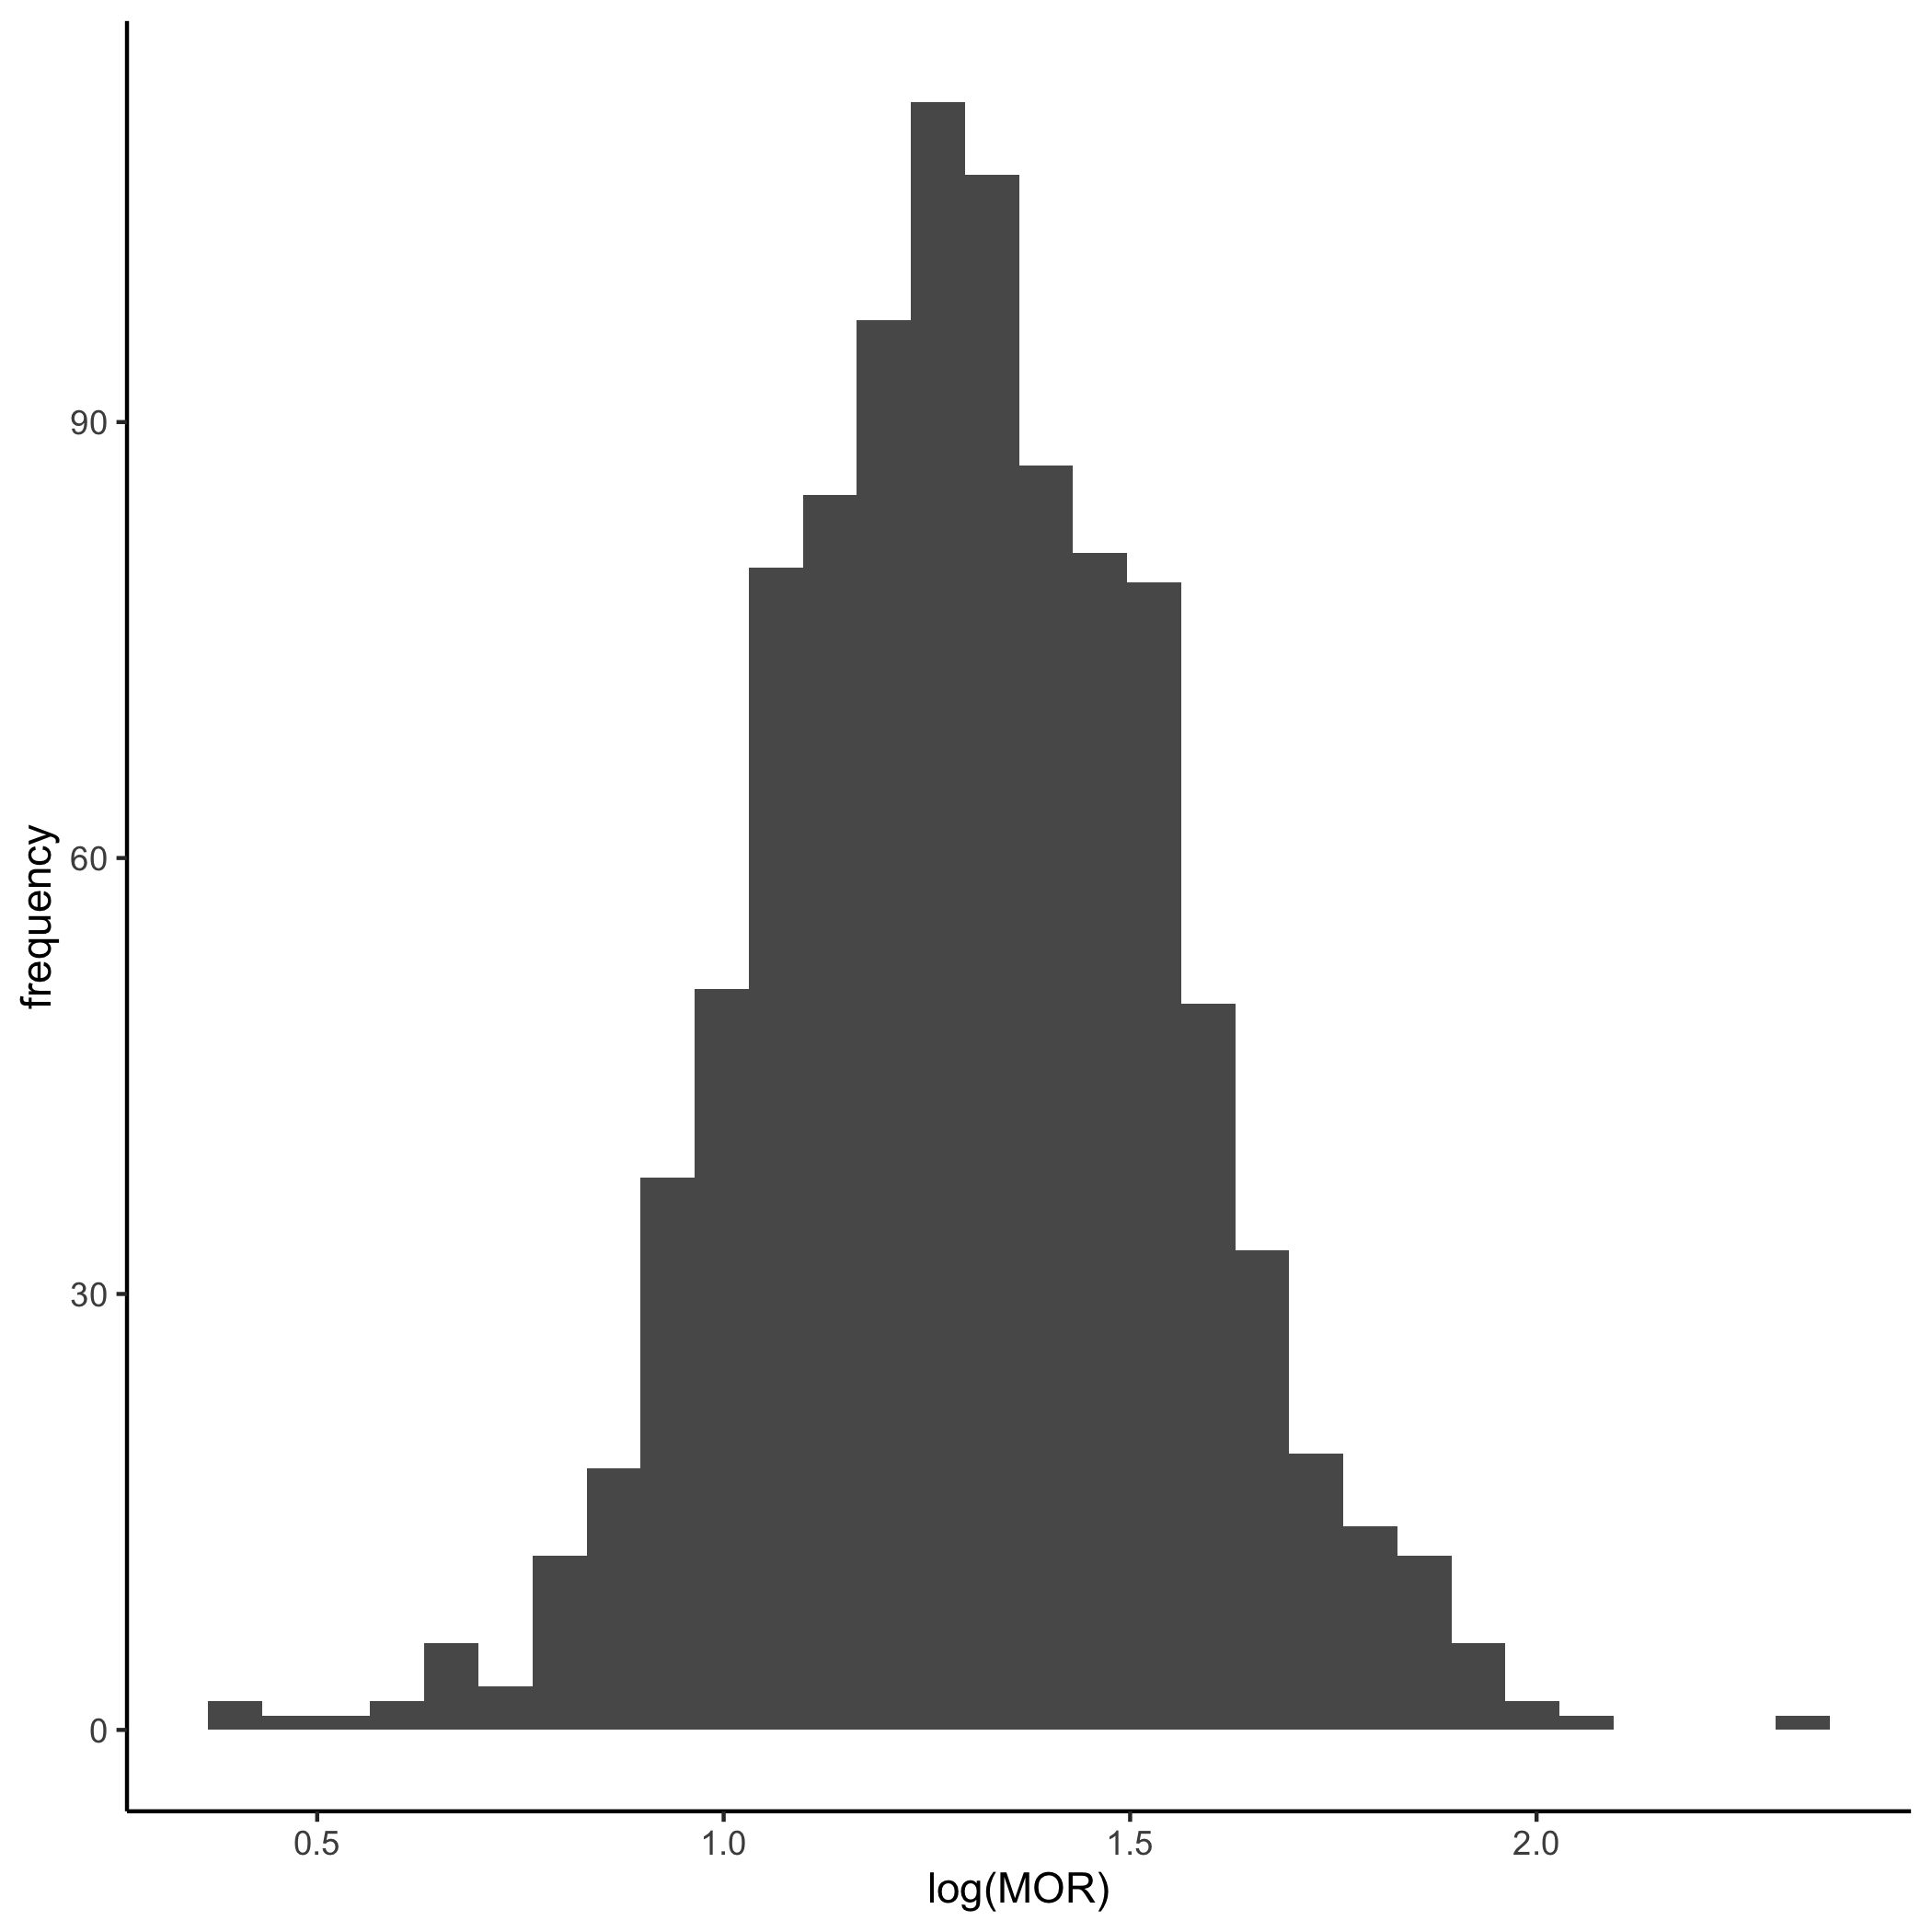
\includegraphics{../../plots/two-lvl-ran-slope/high-prev/hist_100_10_two_lvl_slp_high_prev_q1.png}

}

\caption{Cluster size 10}

}

\end{minipage}%
%
\begin{minipage}[t]{0.24\linewidth}

{\centering 

\raisebox{-\height}{

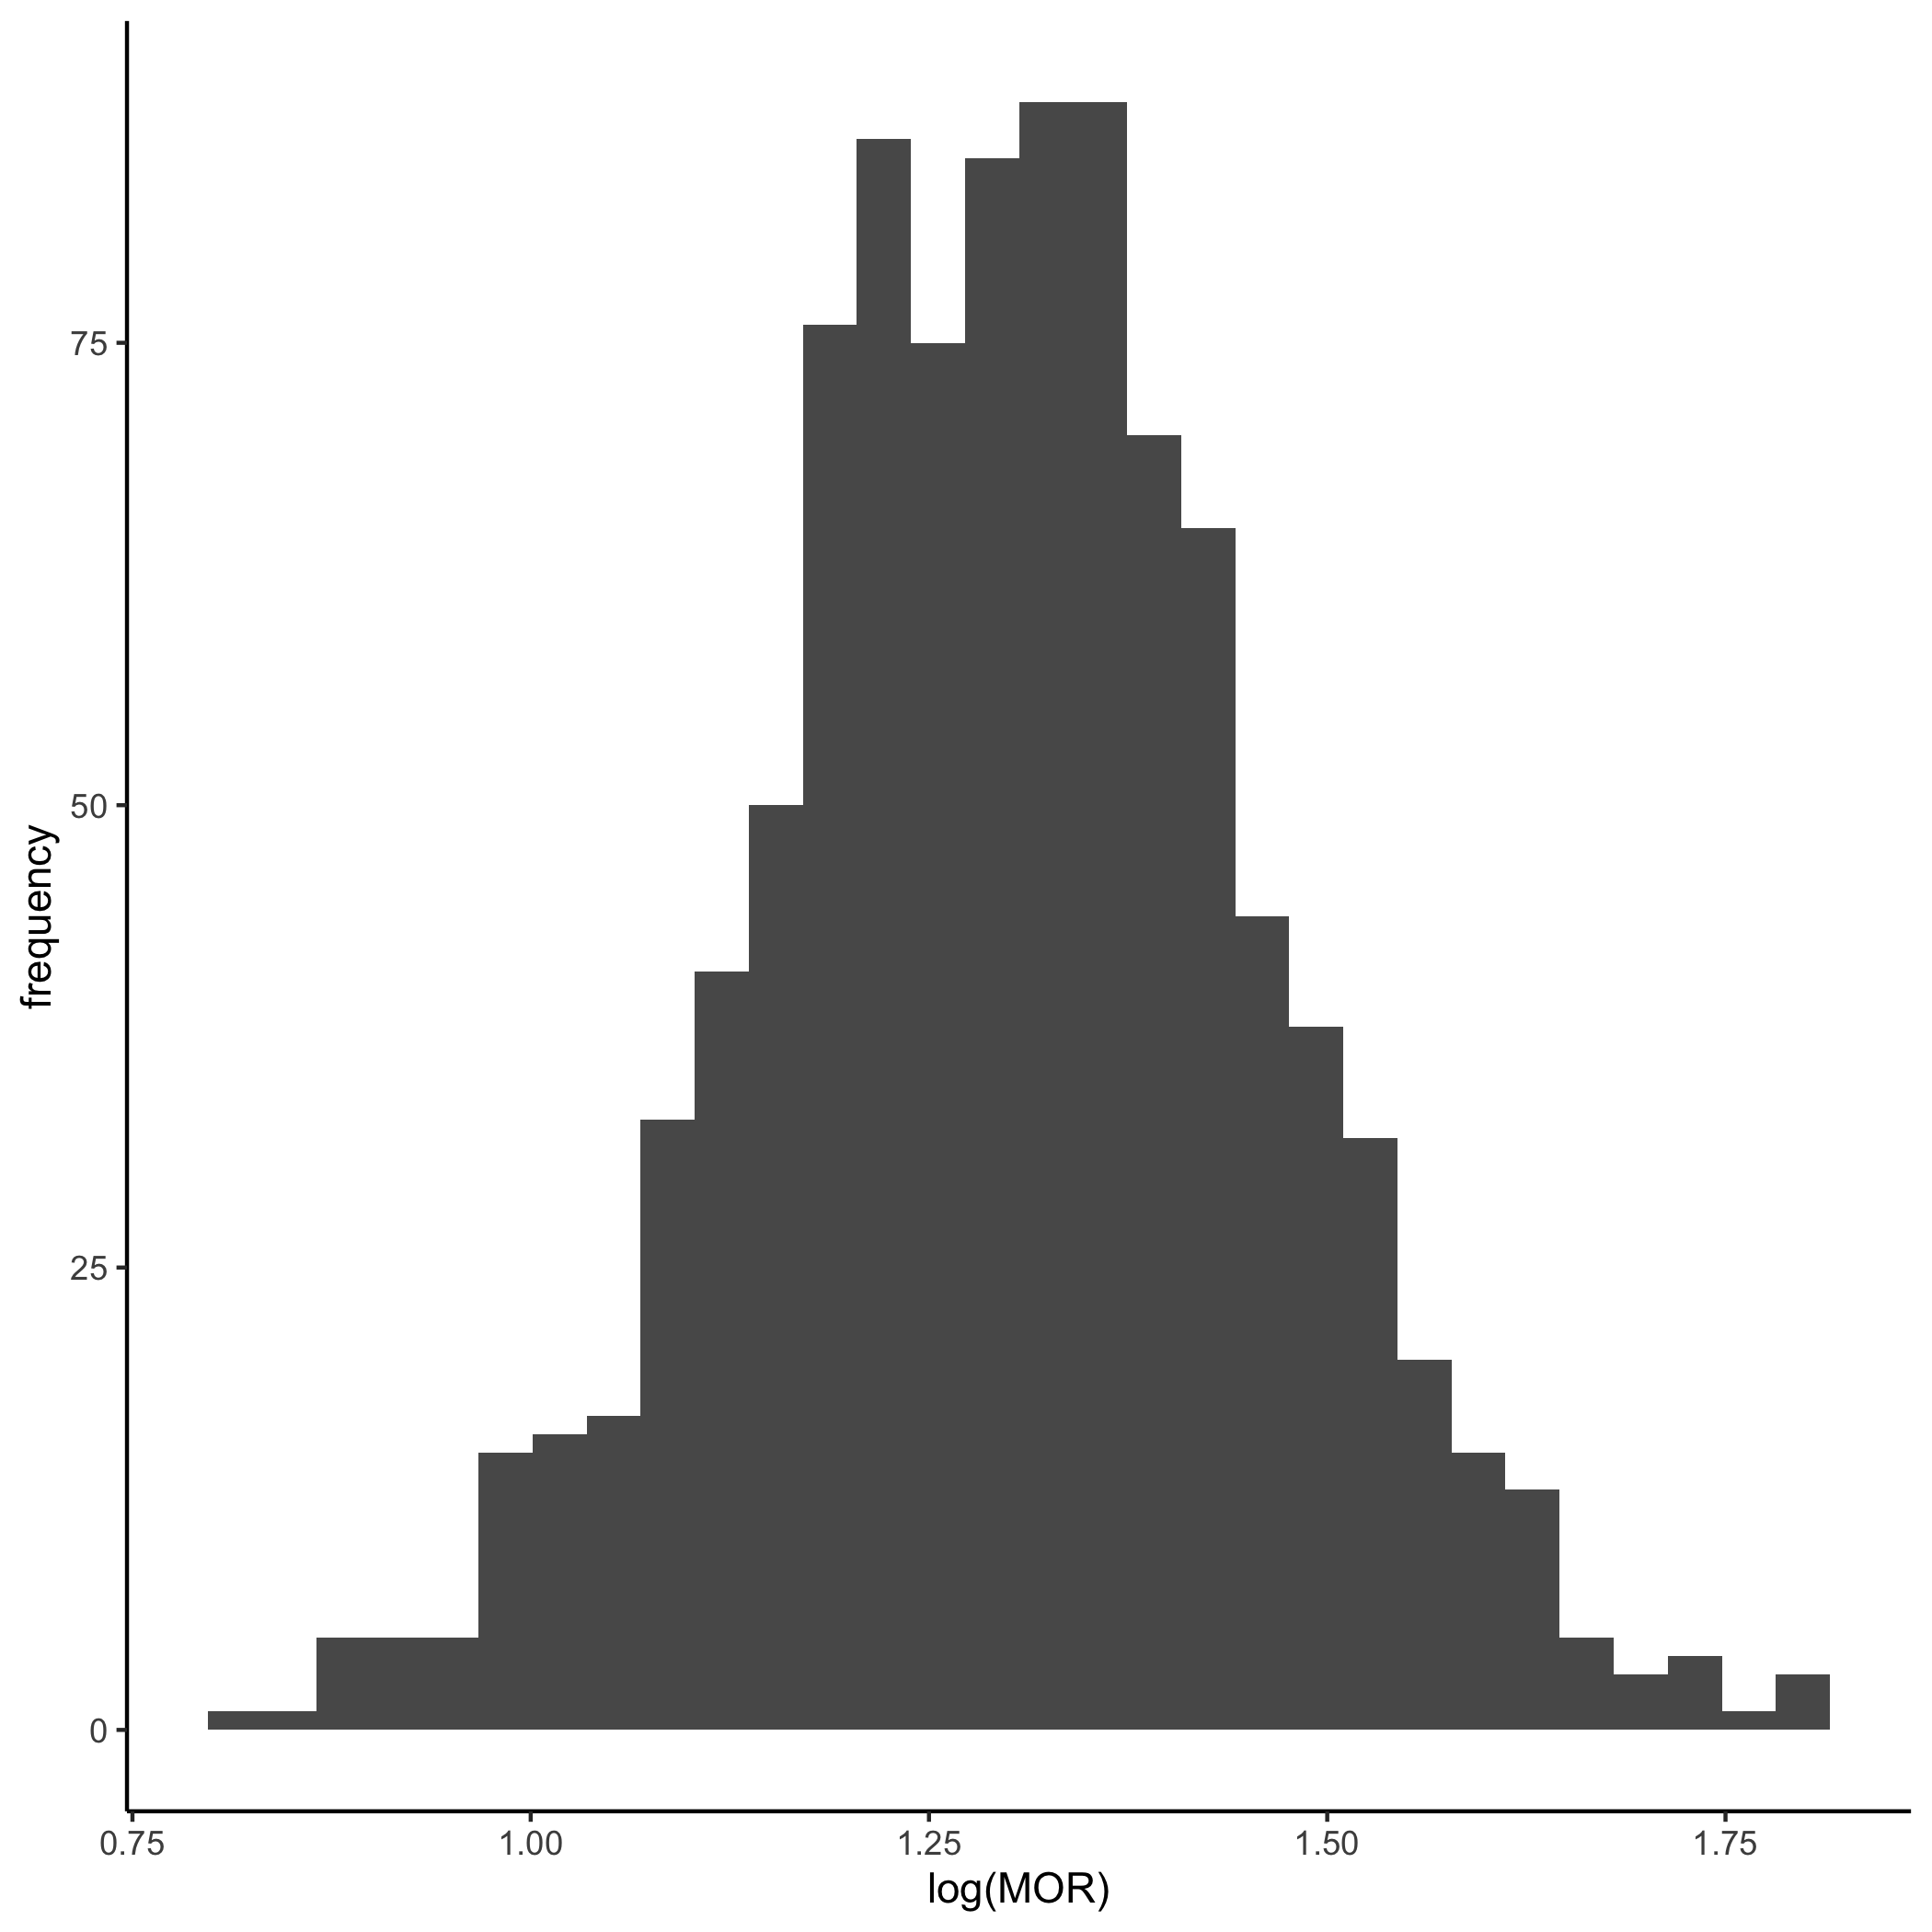
\includegraphics{../../plots/two-lvl-ran-slope/high-prev/hist_100_30_two_lvl_slp_high_prev_q1.png}

}

\caption{Cluster size 30}

}

\end{minipage}%
%
\begin{minipage}[t]{0.24\linewidth}

{\centering 

\raisebox{-\height}{

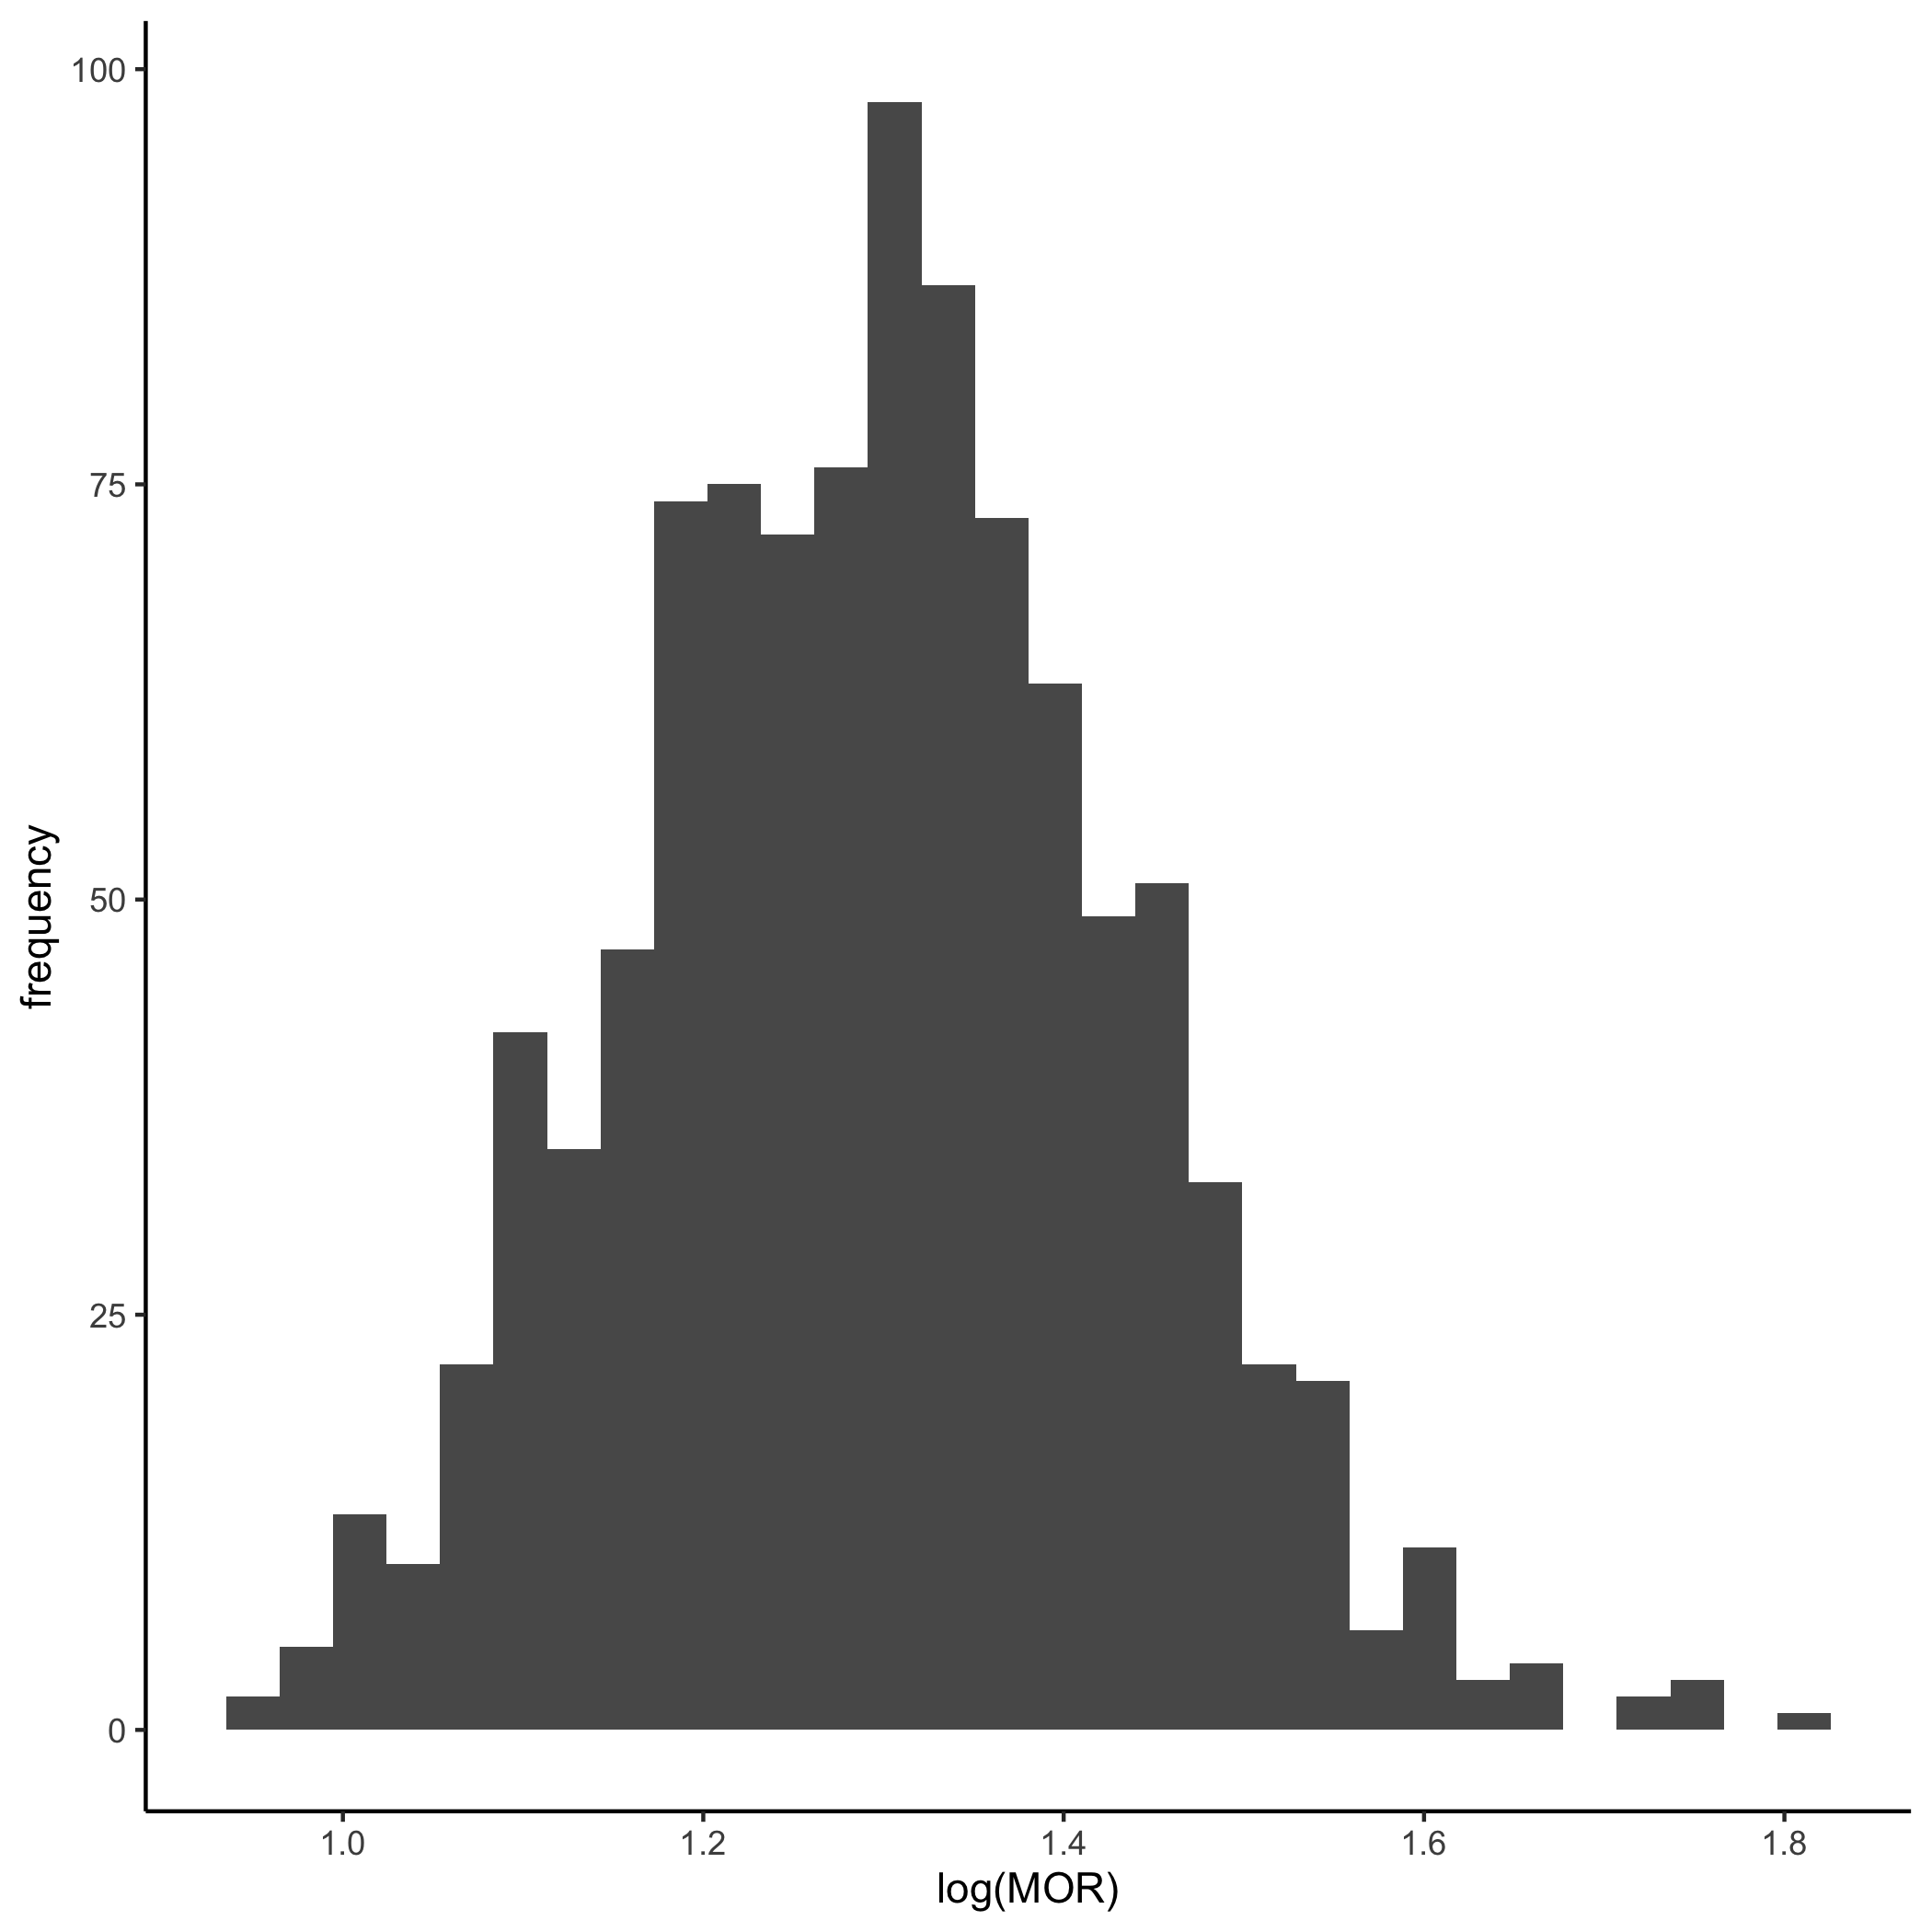
\includegraphics{../../plots/two-lvl-ran-slope/high-prev/hist_100_50_two_lvl_slp_high_prev_q1.png}

}

\caption{Cluster size 50}

}

\end{minipage}%

\end{figure}

\newpage

\hypertarget{histograms-for-logwidehatmor-when-mean-of-x-is-used}{%
\section{\texorpdfstring{Histograms for \(log(\widehat{MOR})\) when Mean
of \(X\) is
used}{Histograms for log(\textbackslash widehat\{MOR\}) when Mean of X is used}}\label{histograms-for-logwidehatmor-when-mean-of-x-is-used}}

\vspace{10mm}

\begin{figure}

\begin{minipage}[t]{0.05\linewidth}

{\centering 

\rotatebox[origin=br]{90}{\tiny Cluster Number 10}

}

\end{minipage}%
%
\begin{minipage}[t]{0.24\linewidth}

{\centering 

\raisebox{-\height}{

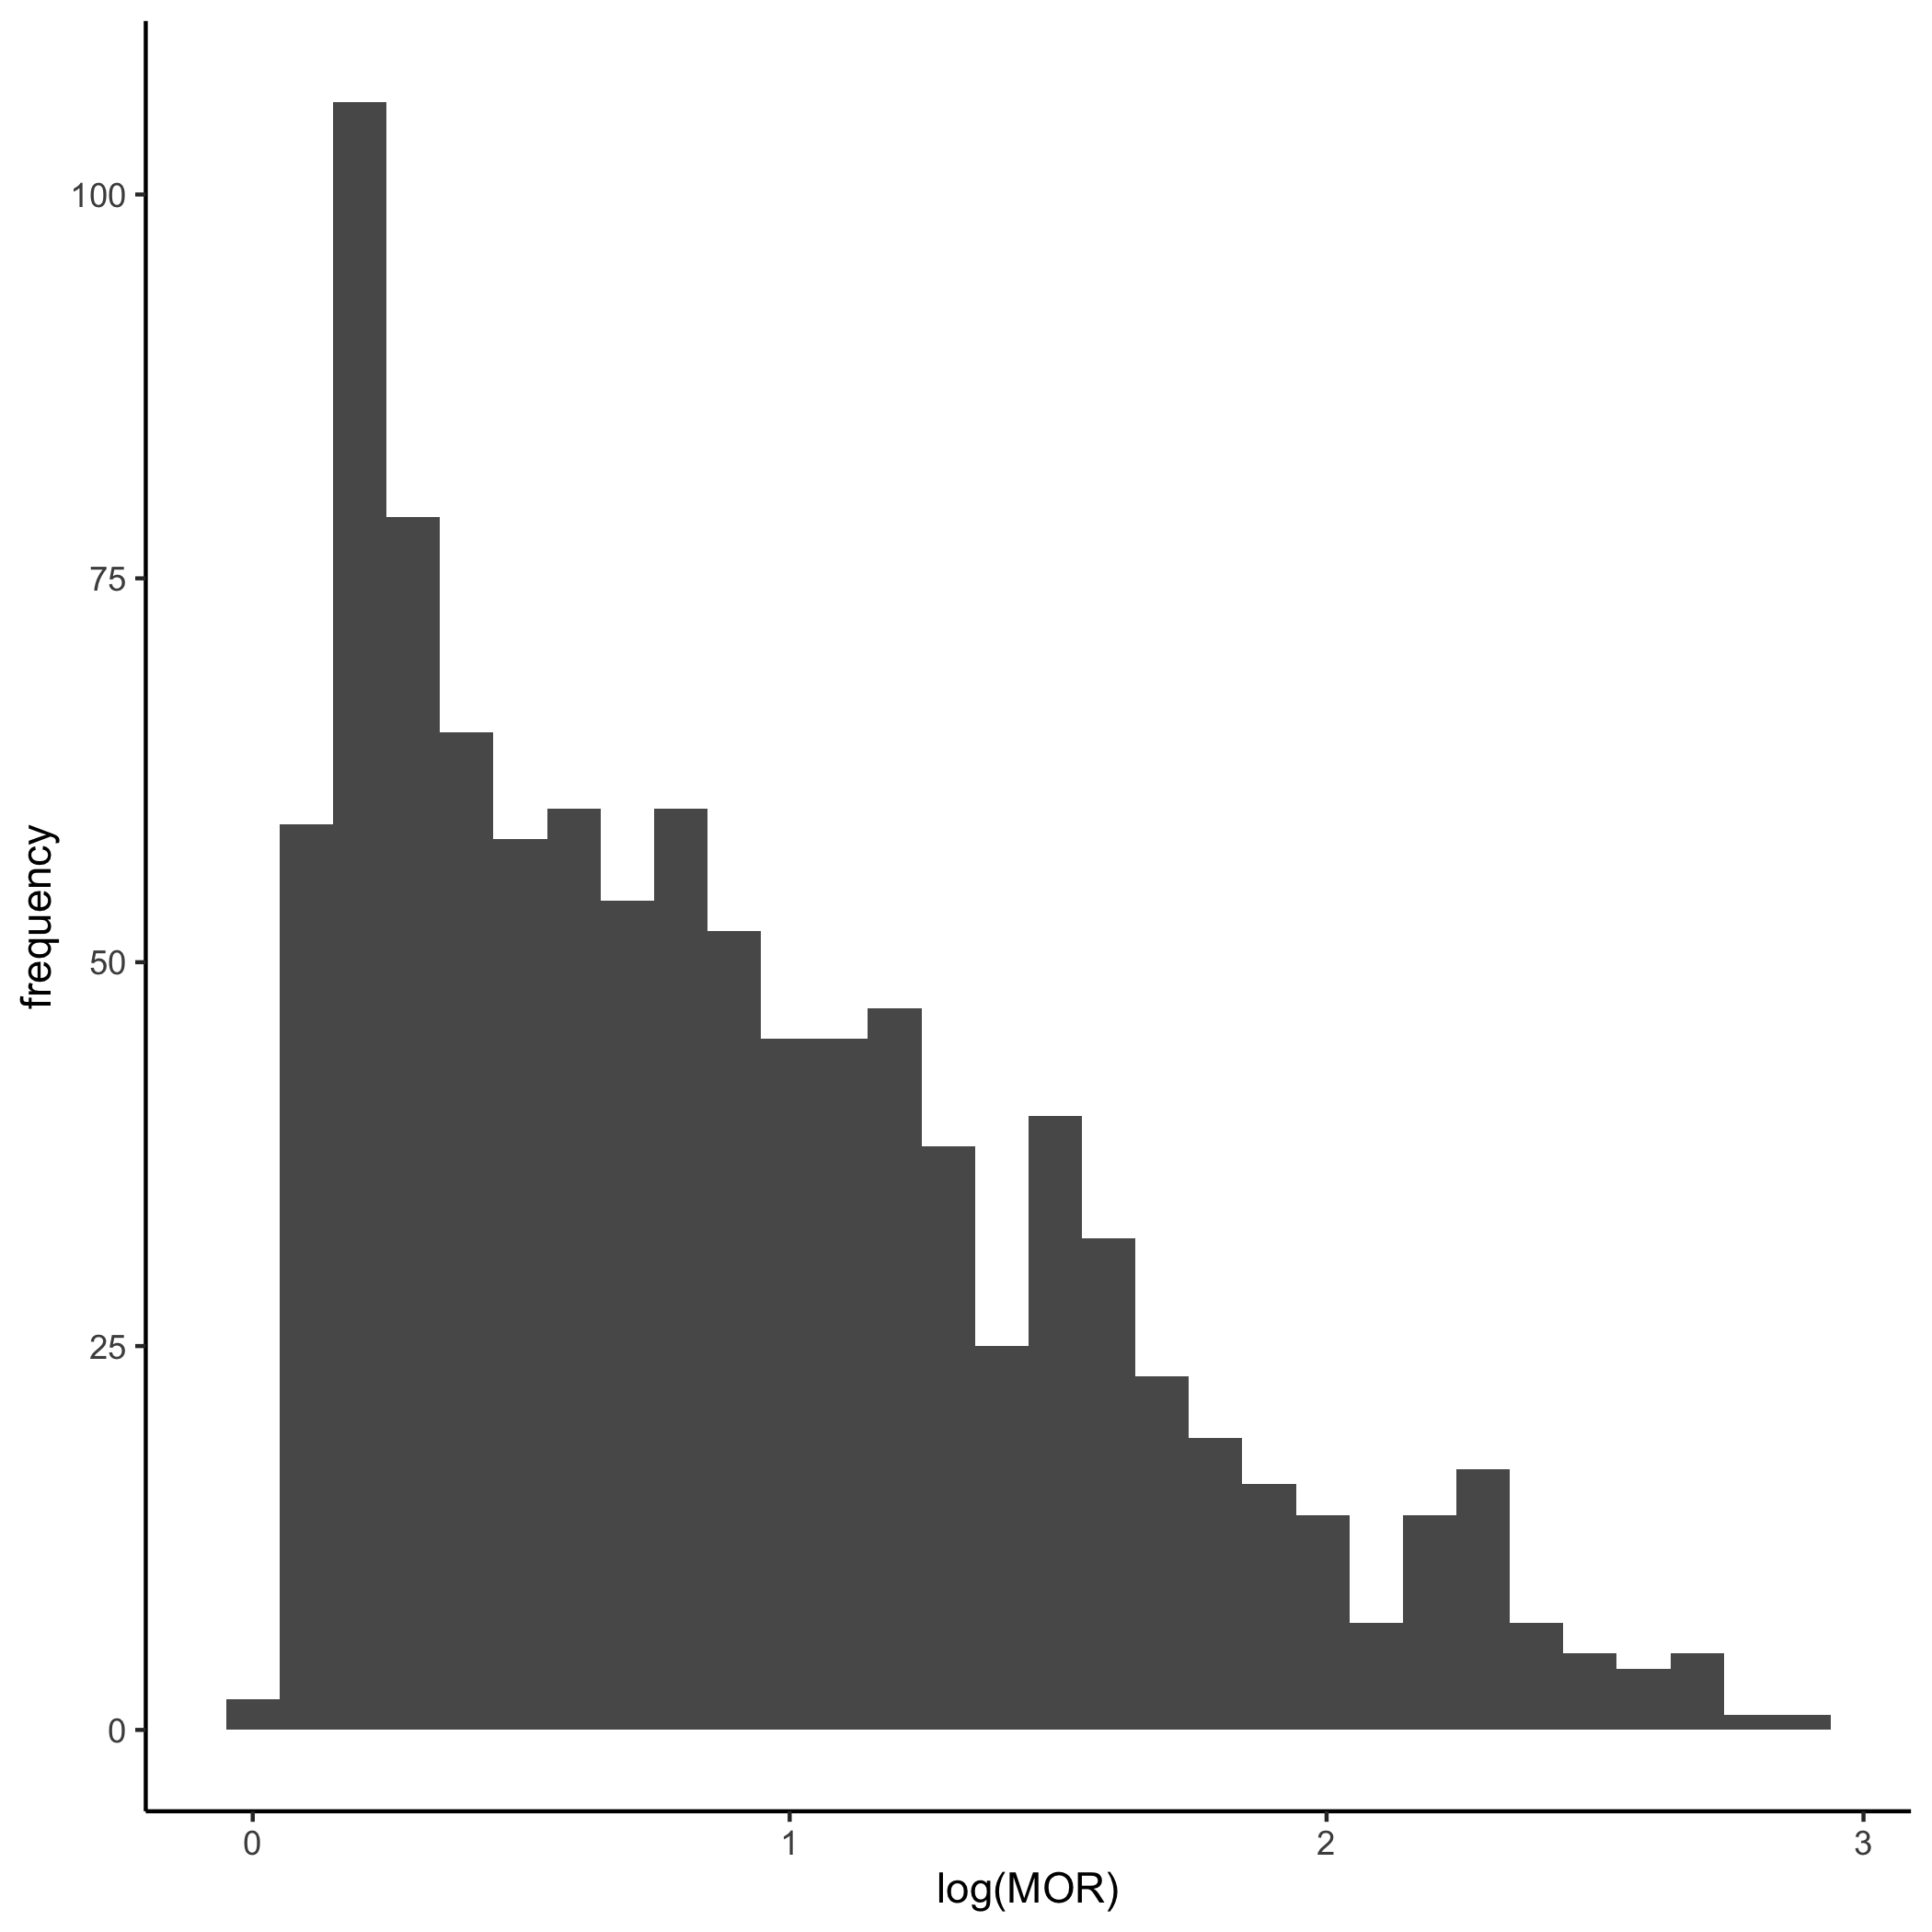
\includegraphics{../../plots/two-lvl-ran-slope/high-prev/hist_10_5_two_lvl_slp_high_prev_q2.png}

}

\caption{Cluster size 5}

}

\end{minipage}%
%
\begin{minipage}[t]{0.24\linewidth}

{\centering 

\raisebox{-\height}{

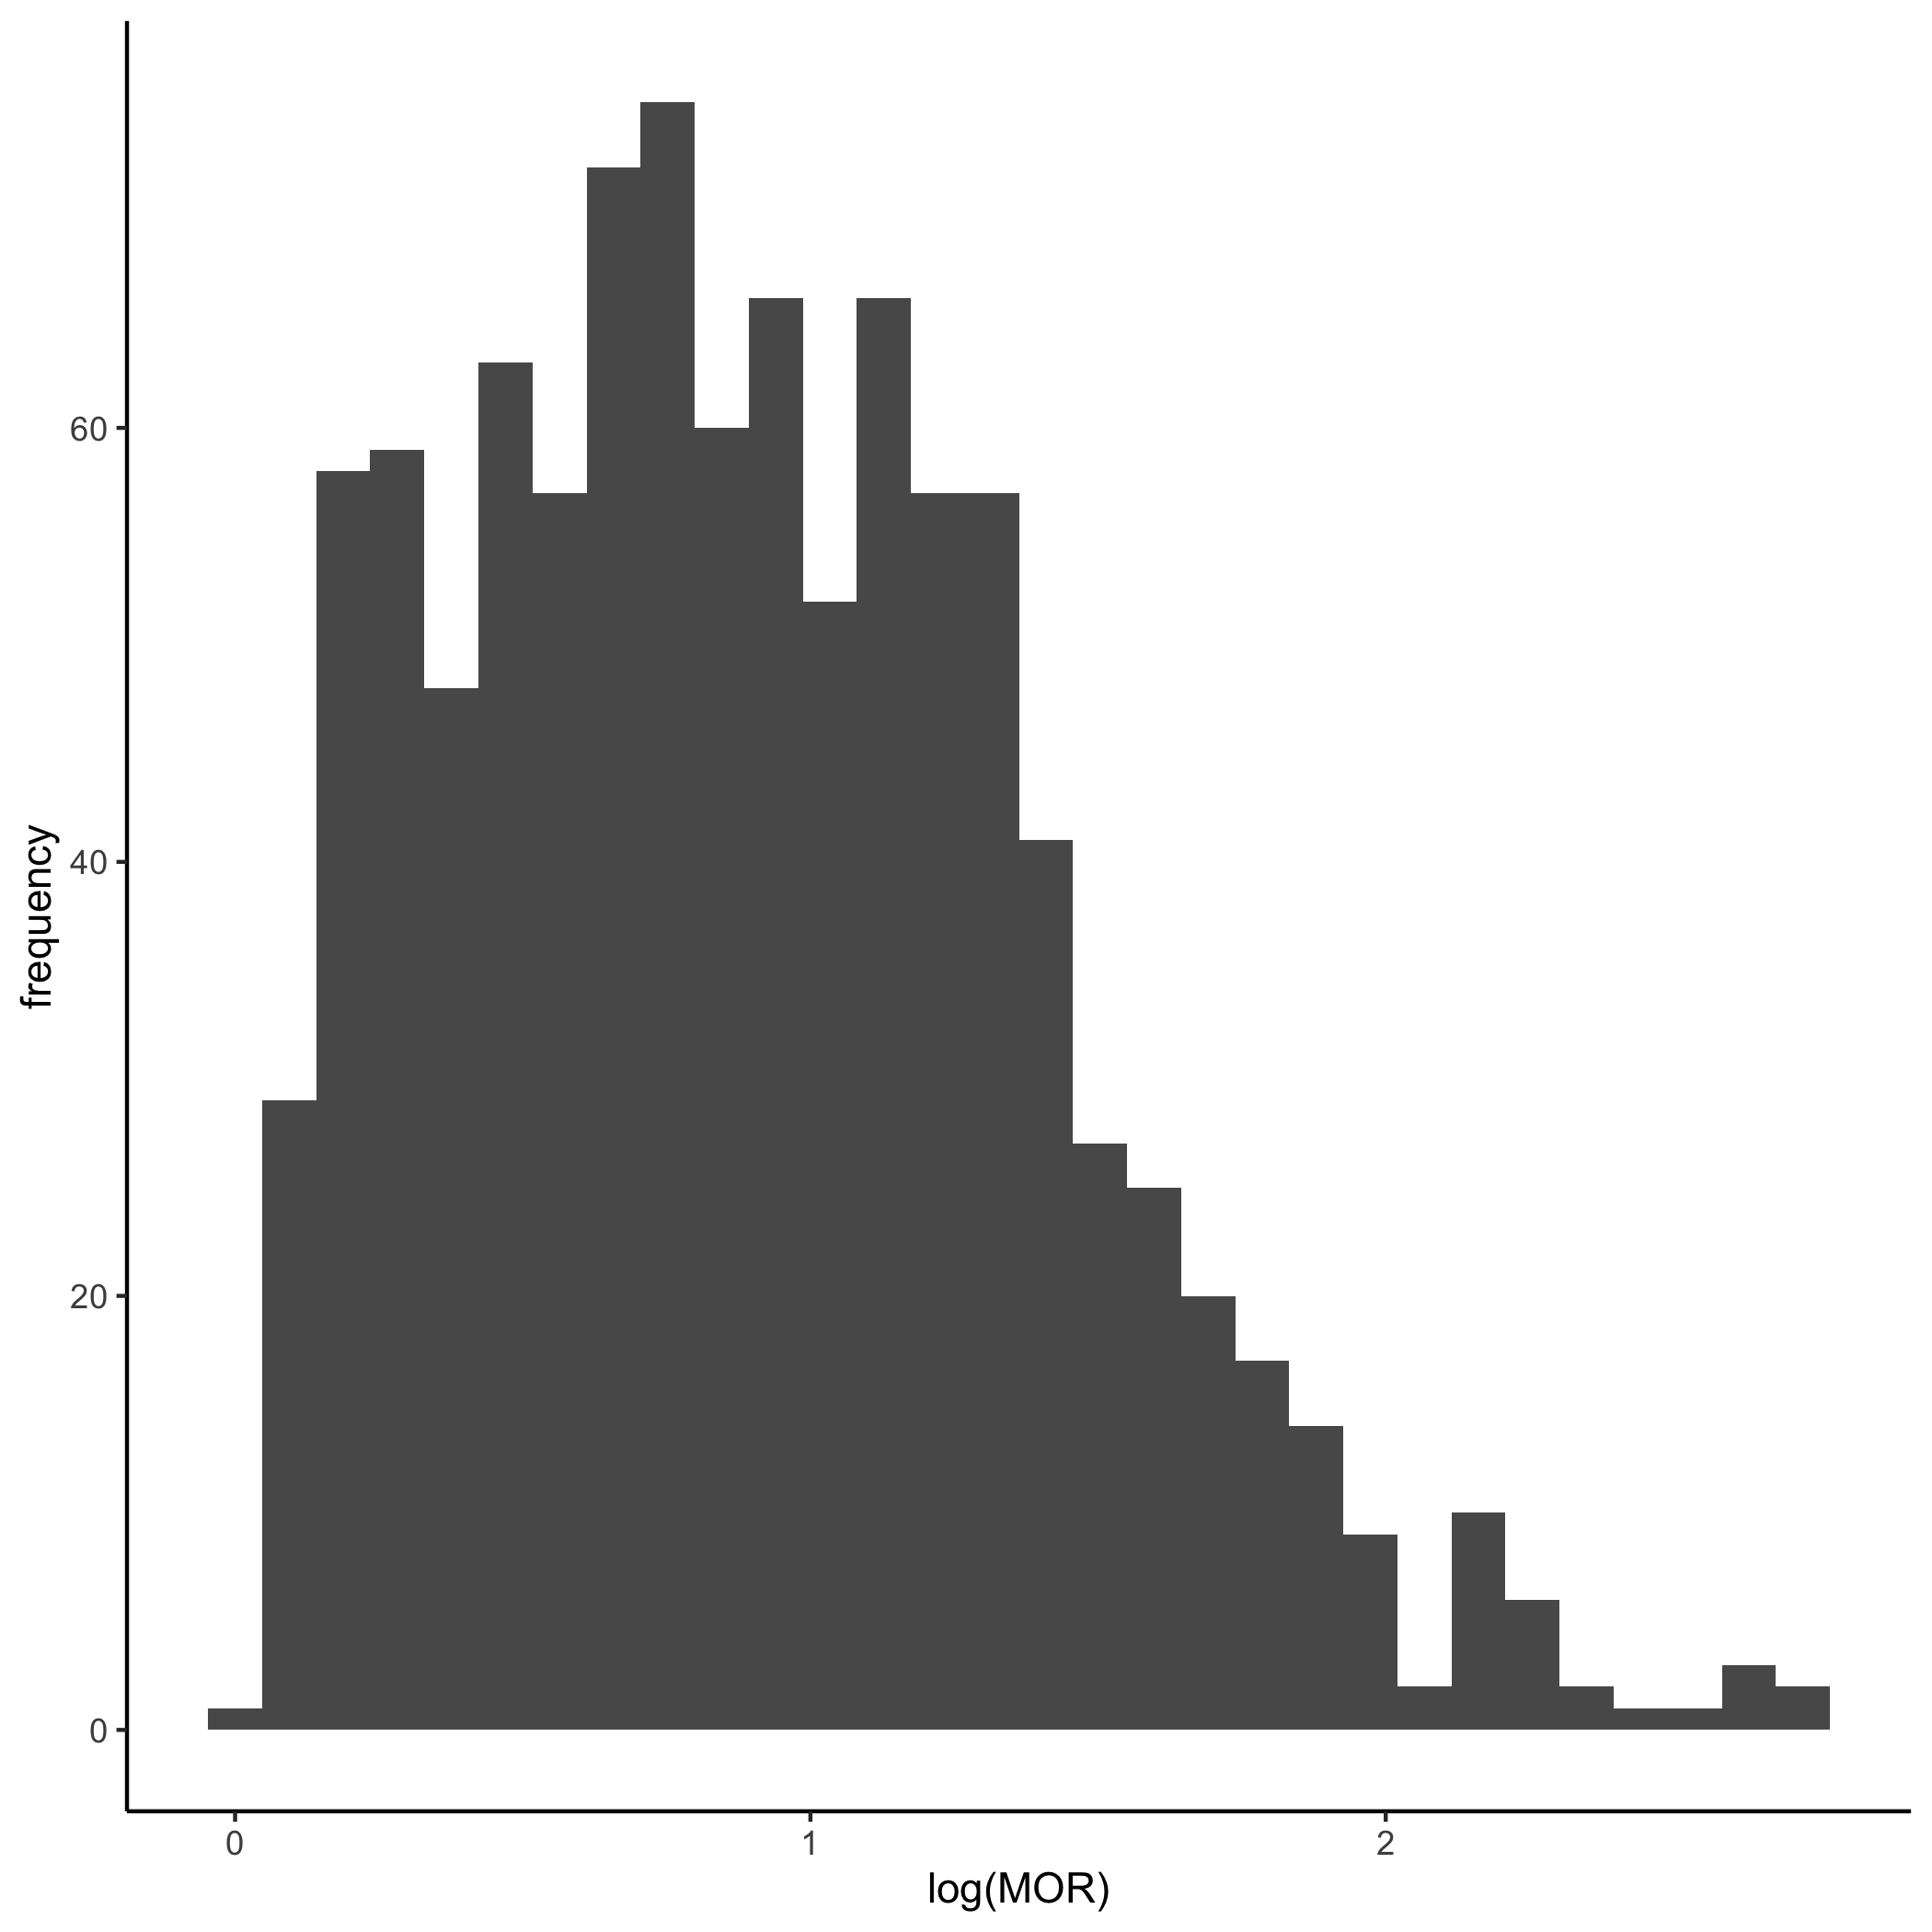
\includegraphics{../../plots/two-lvl-ran-slope/high-prev/hist_10_10_two_lvl_slp_high_prev_q2.png}

}

\caption{Cluster size 10}

}

\end{minipage}%
%
\begin{minipage}[t]{0.24\linewidth}

{\centering 

\raisebox{-\height}{

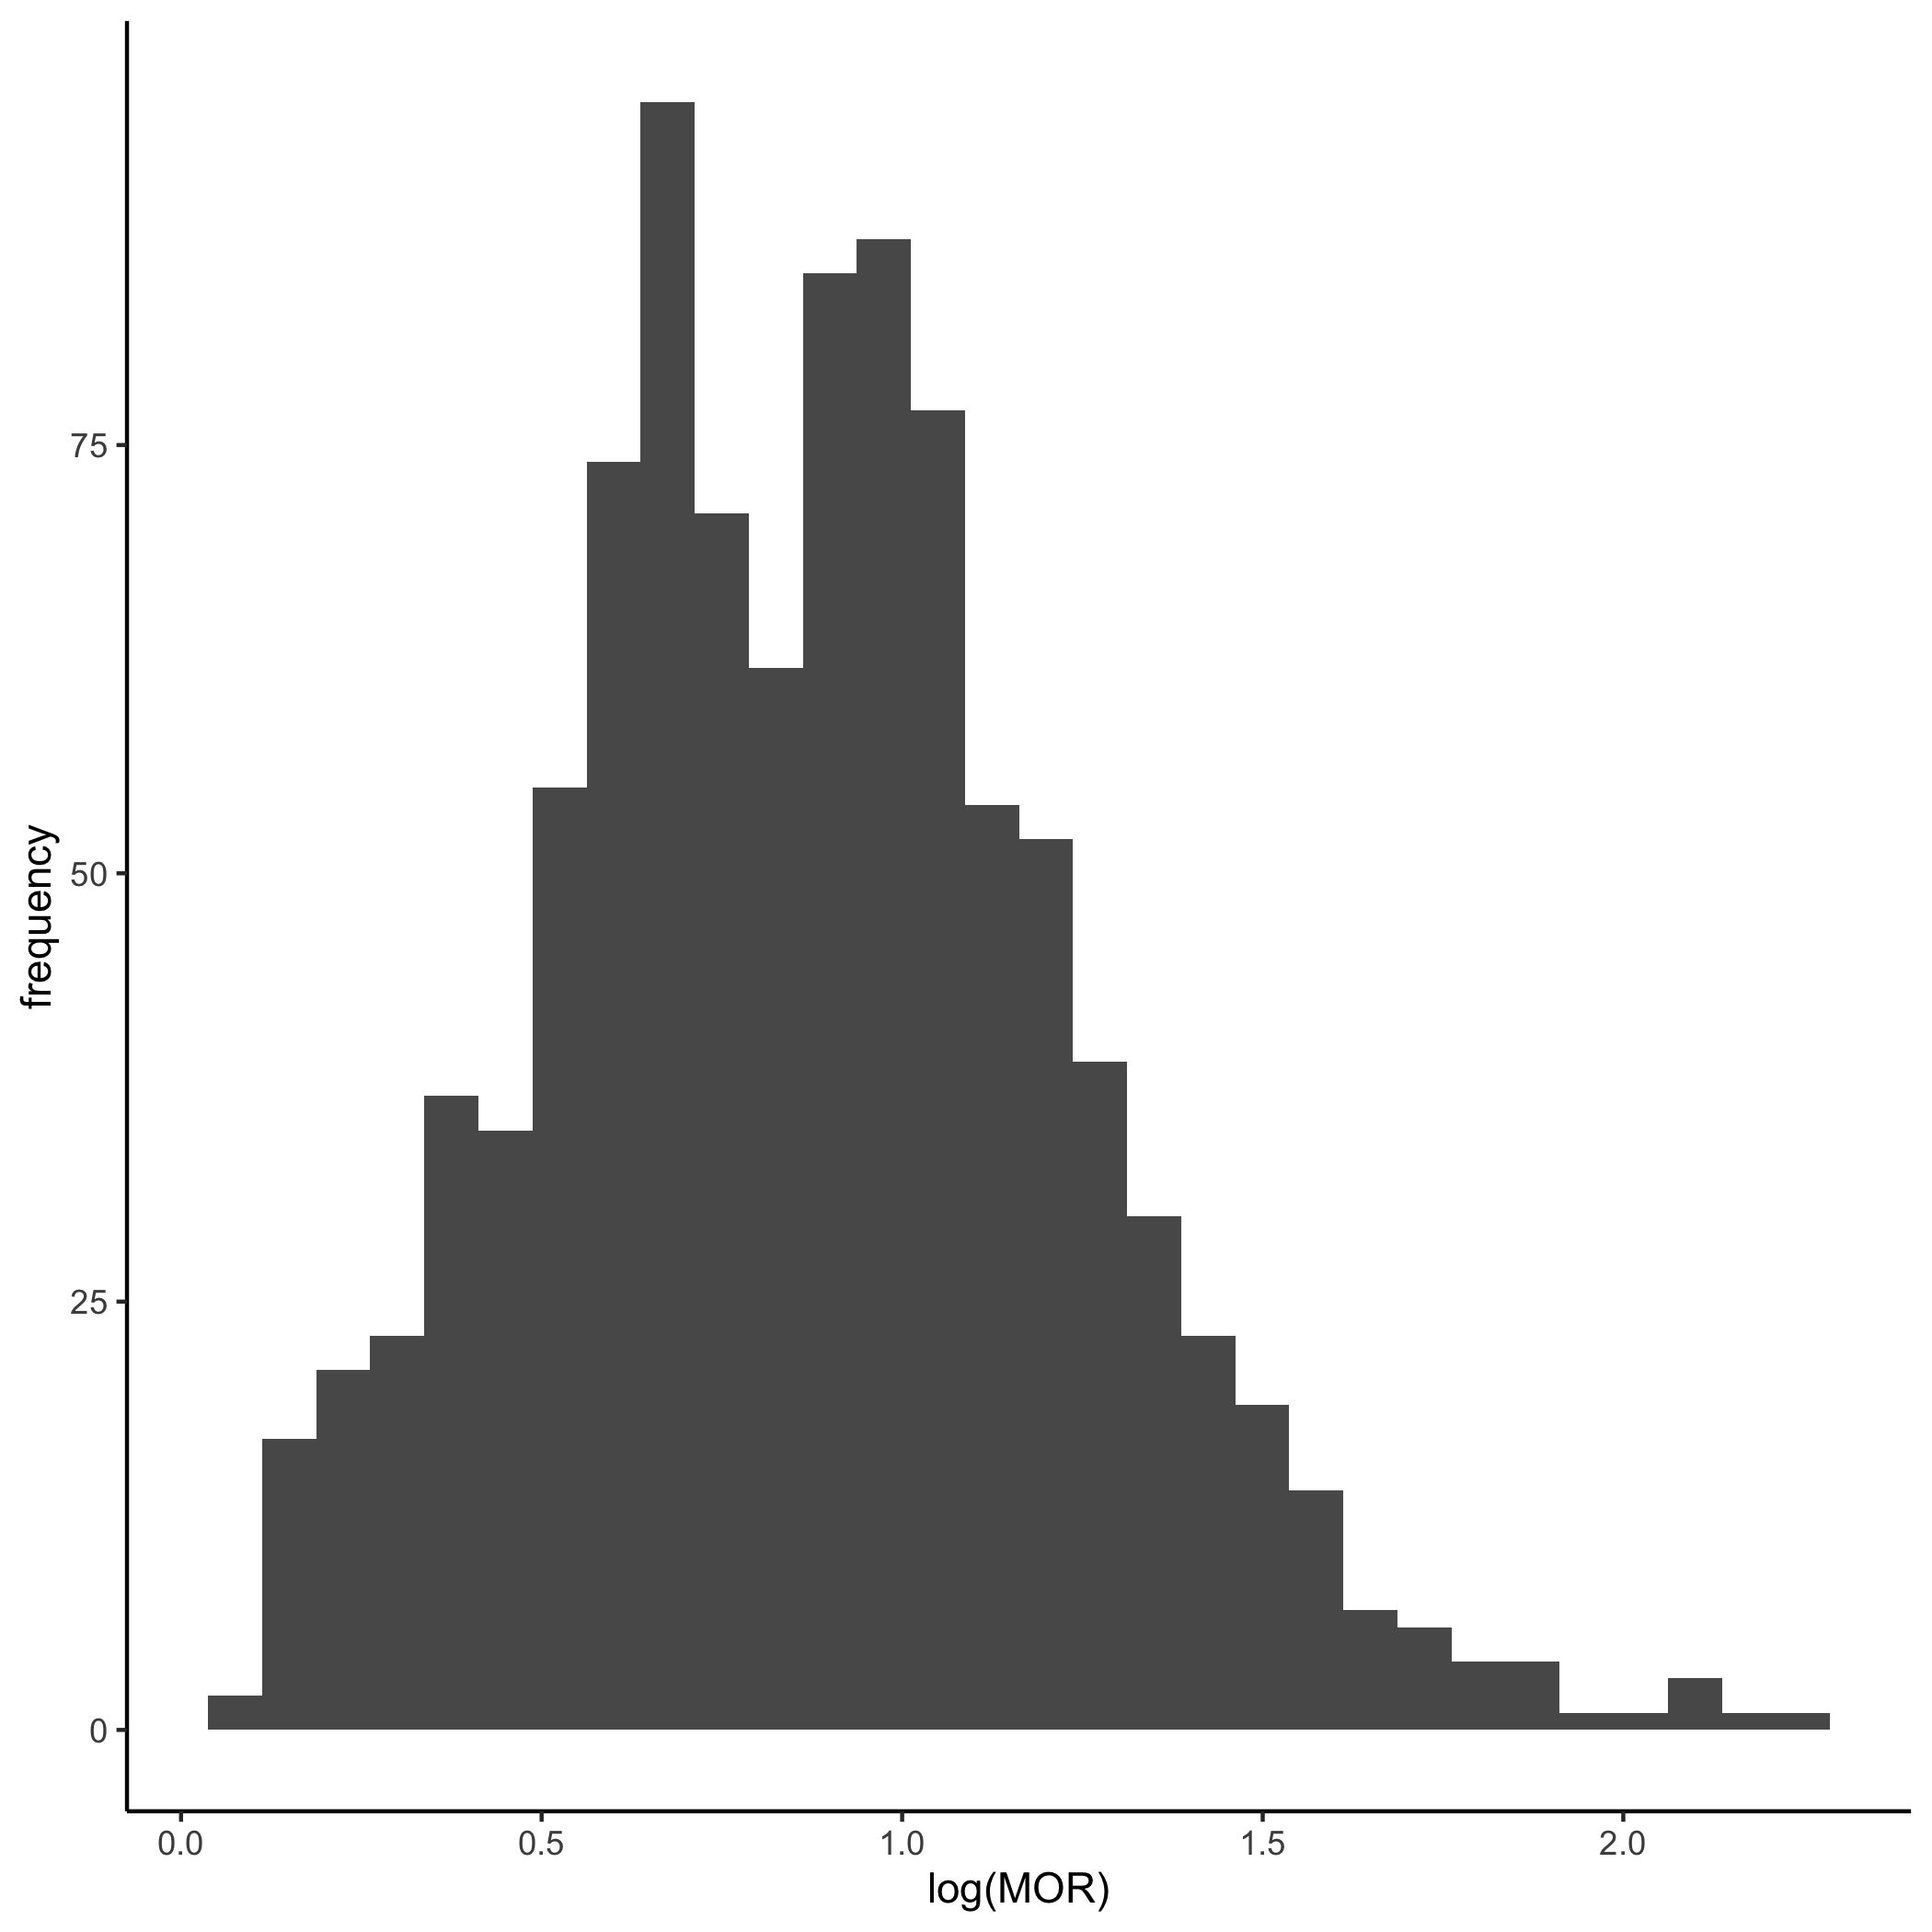
\includegraphics{../../plots/two-lvl-ran-slope/high-prev/hist_10_30_two_lvl_slp_high_prev_q2.png}

}

\caption{Cluster size 30}

}

\end{minipage}%
%
\begin{minipage}[t]{0.24\linewidth}

{\centering 

\raisebox{-\height}{

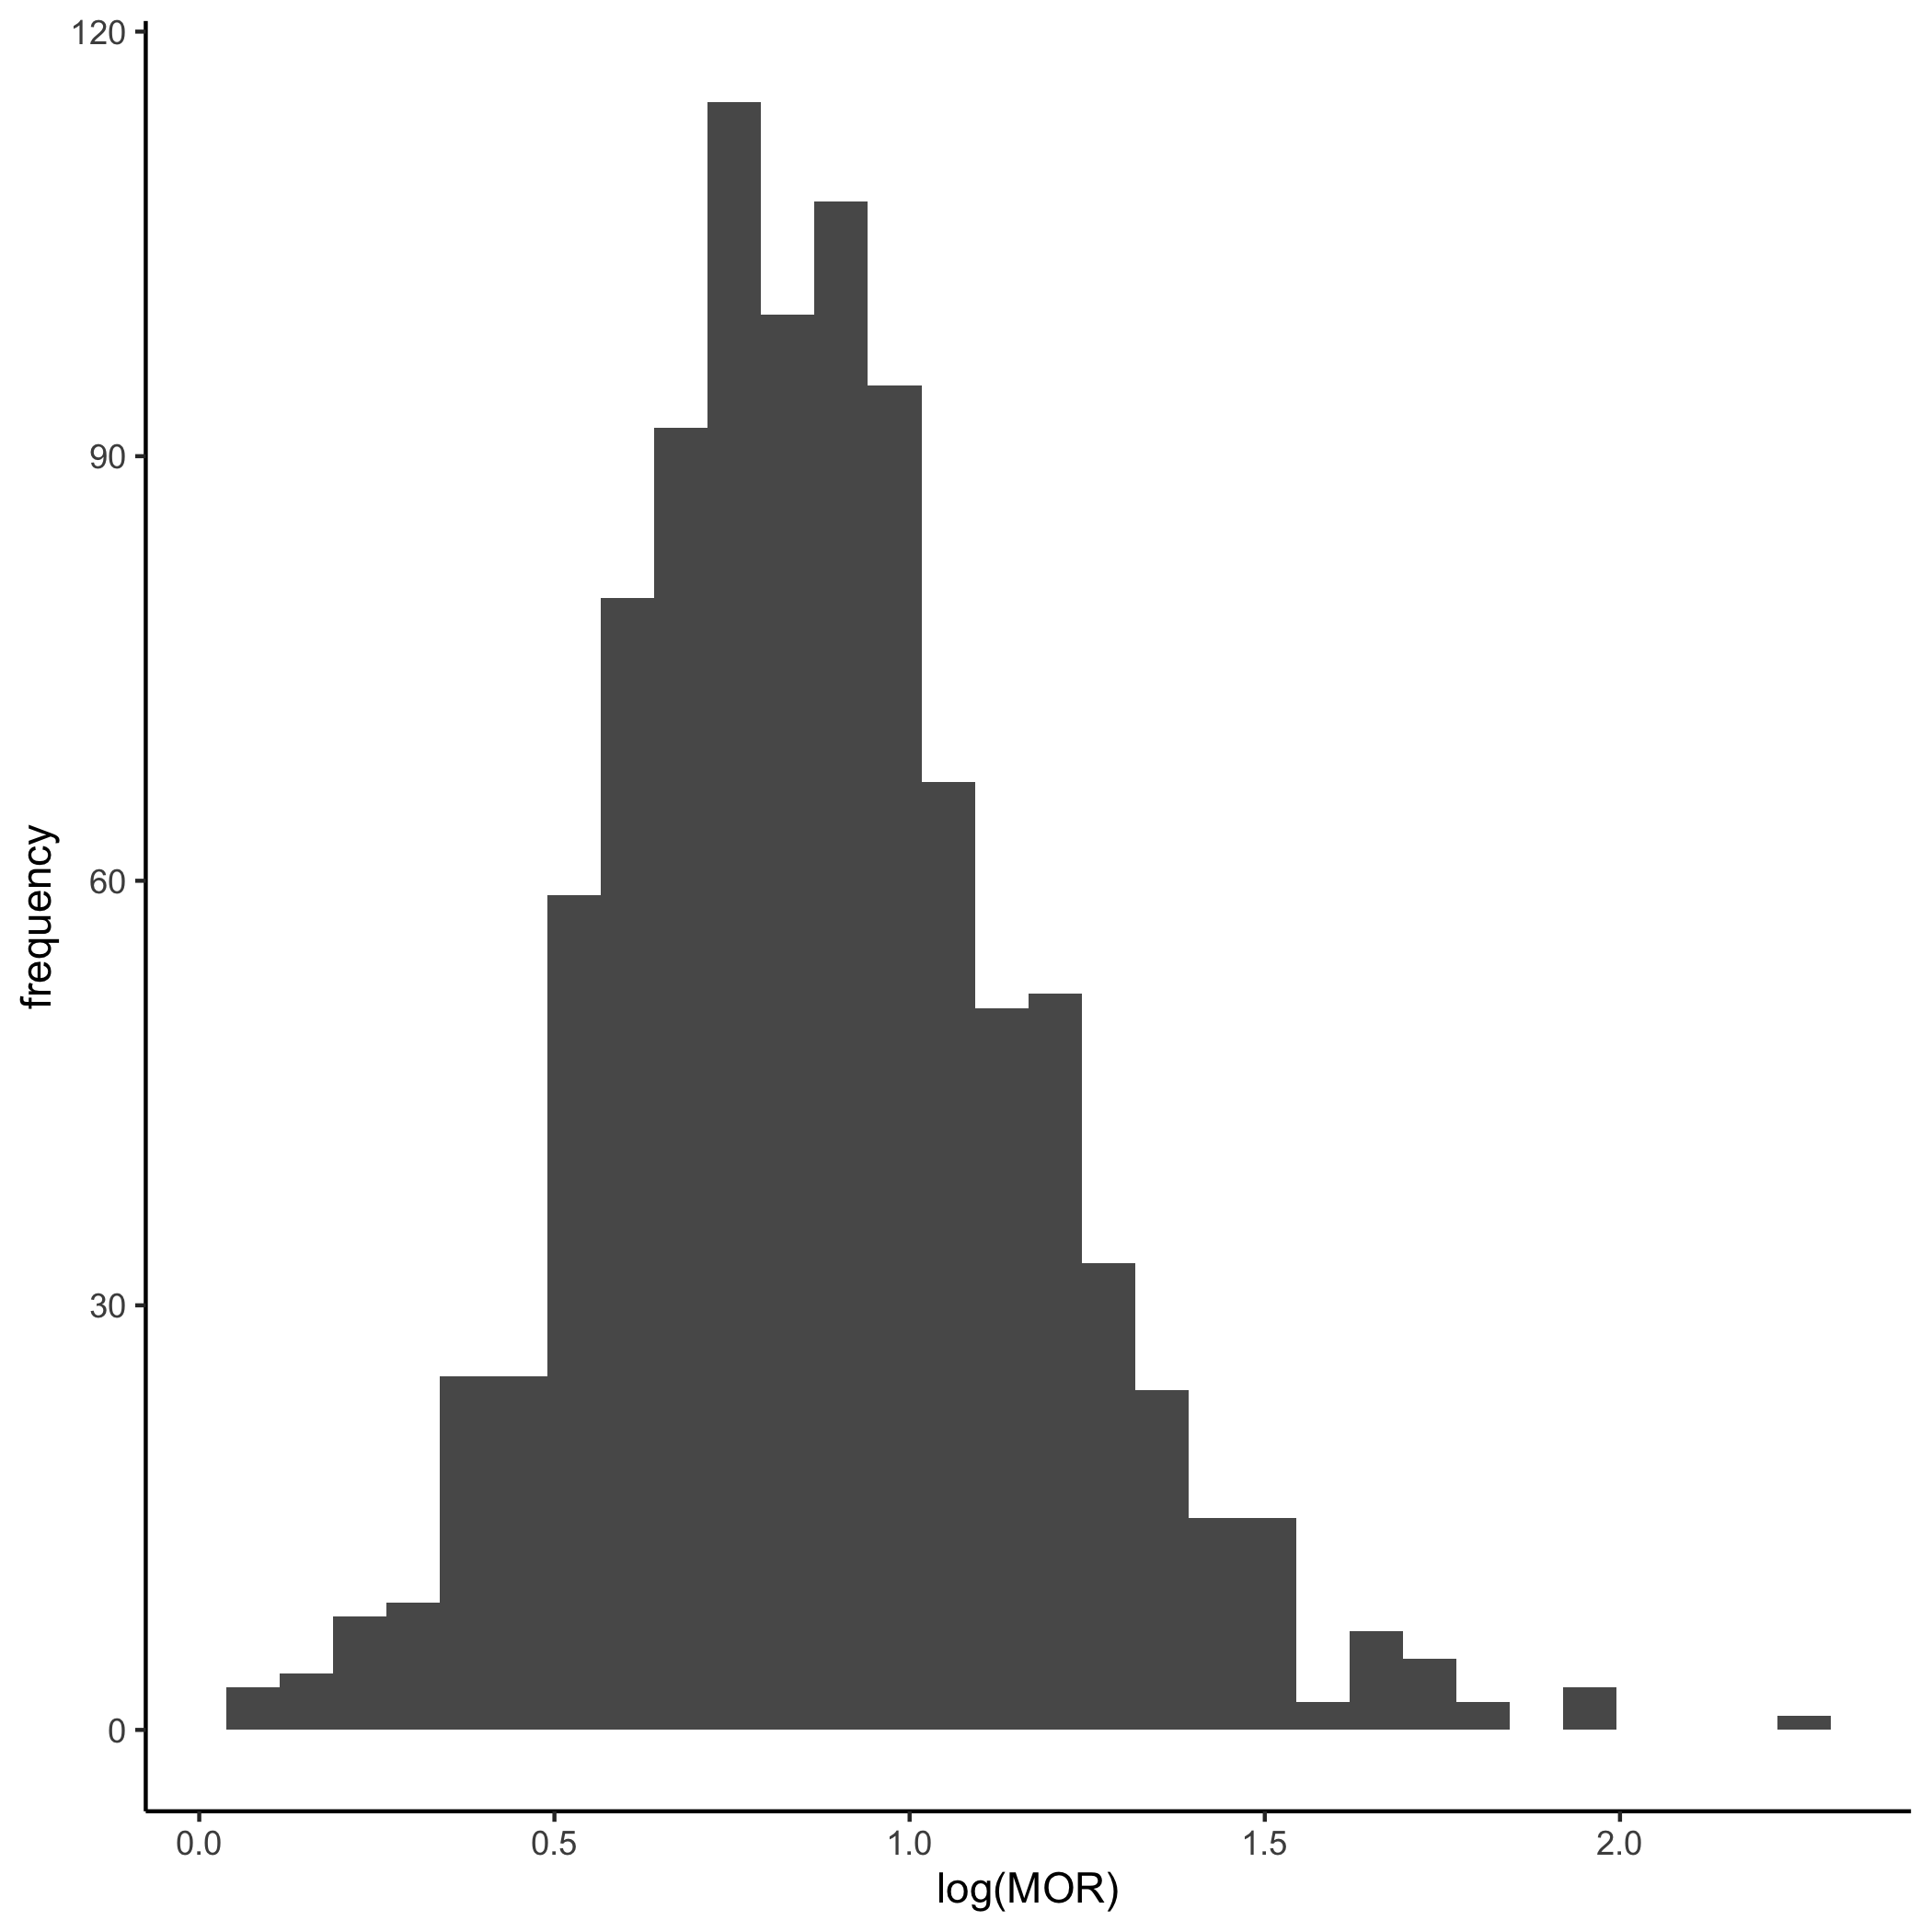
\includegraphics{../../plots/two-lvl-ran-slope/high-prev/hist_10_50_two_lvl_slp_high_prev_q2.png}

}

\caption{Cluster size 50}

}

\end{minipage}%
\newline
\begin{minipage}[t]{\linewidth}

{\centering 

~

}

\end{minipage}%
\newline
\begin{minipage}[t]{0.05\linewidth}

{\centering 

\rotatebox[origin=br]{90}{\tiny Cluster Number 30}

}

\end{minipage}%
%
\begin{minipage}[t]{0.24\linewidth}

{\centering 

\raisebox{-\height}{

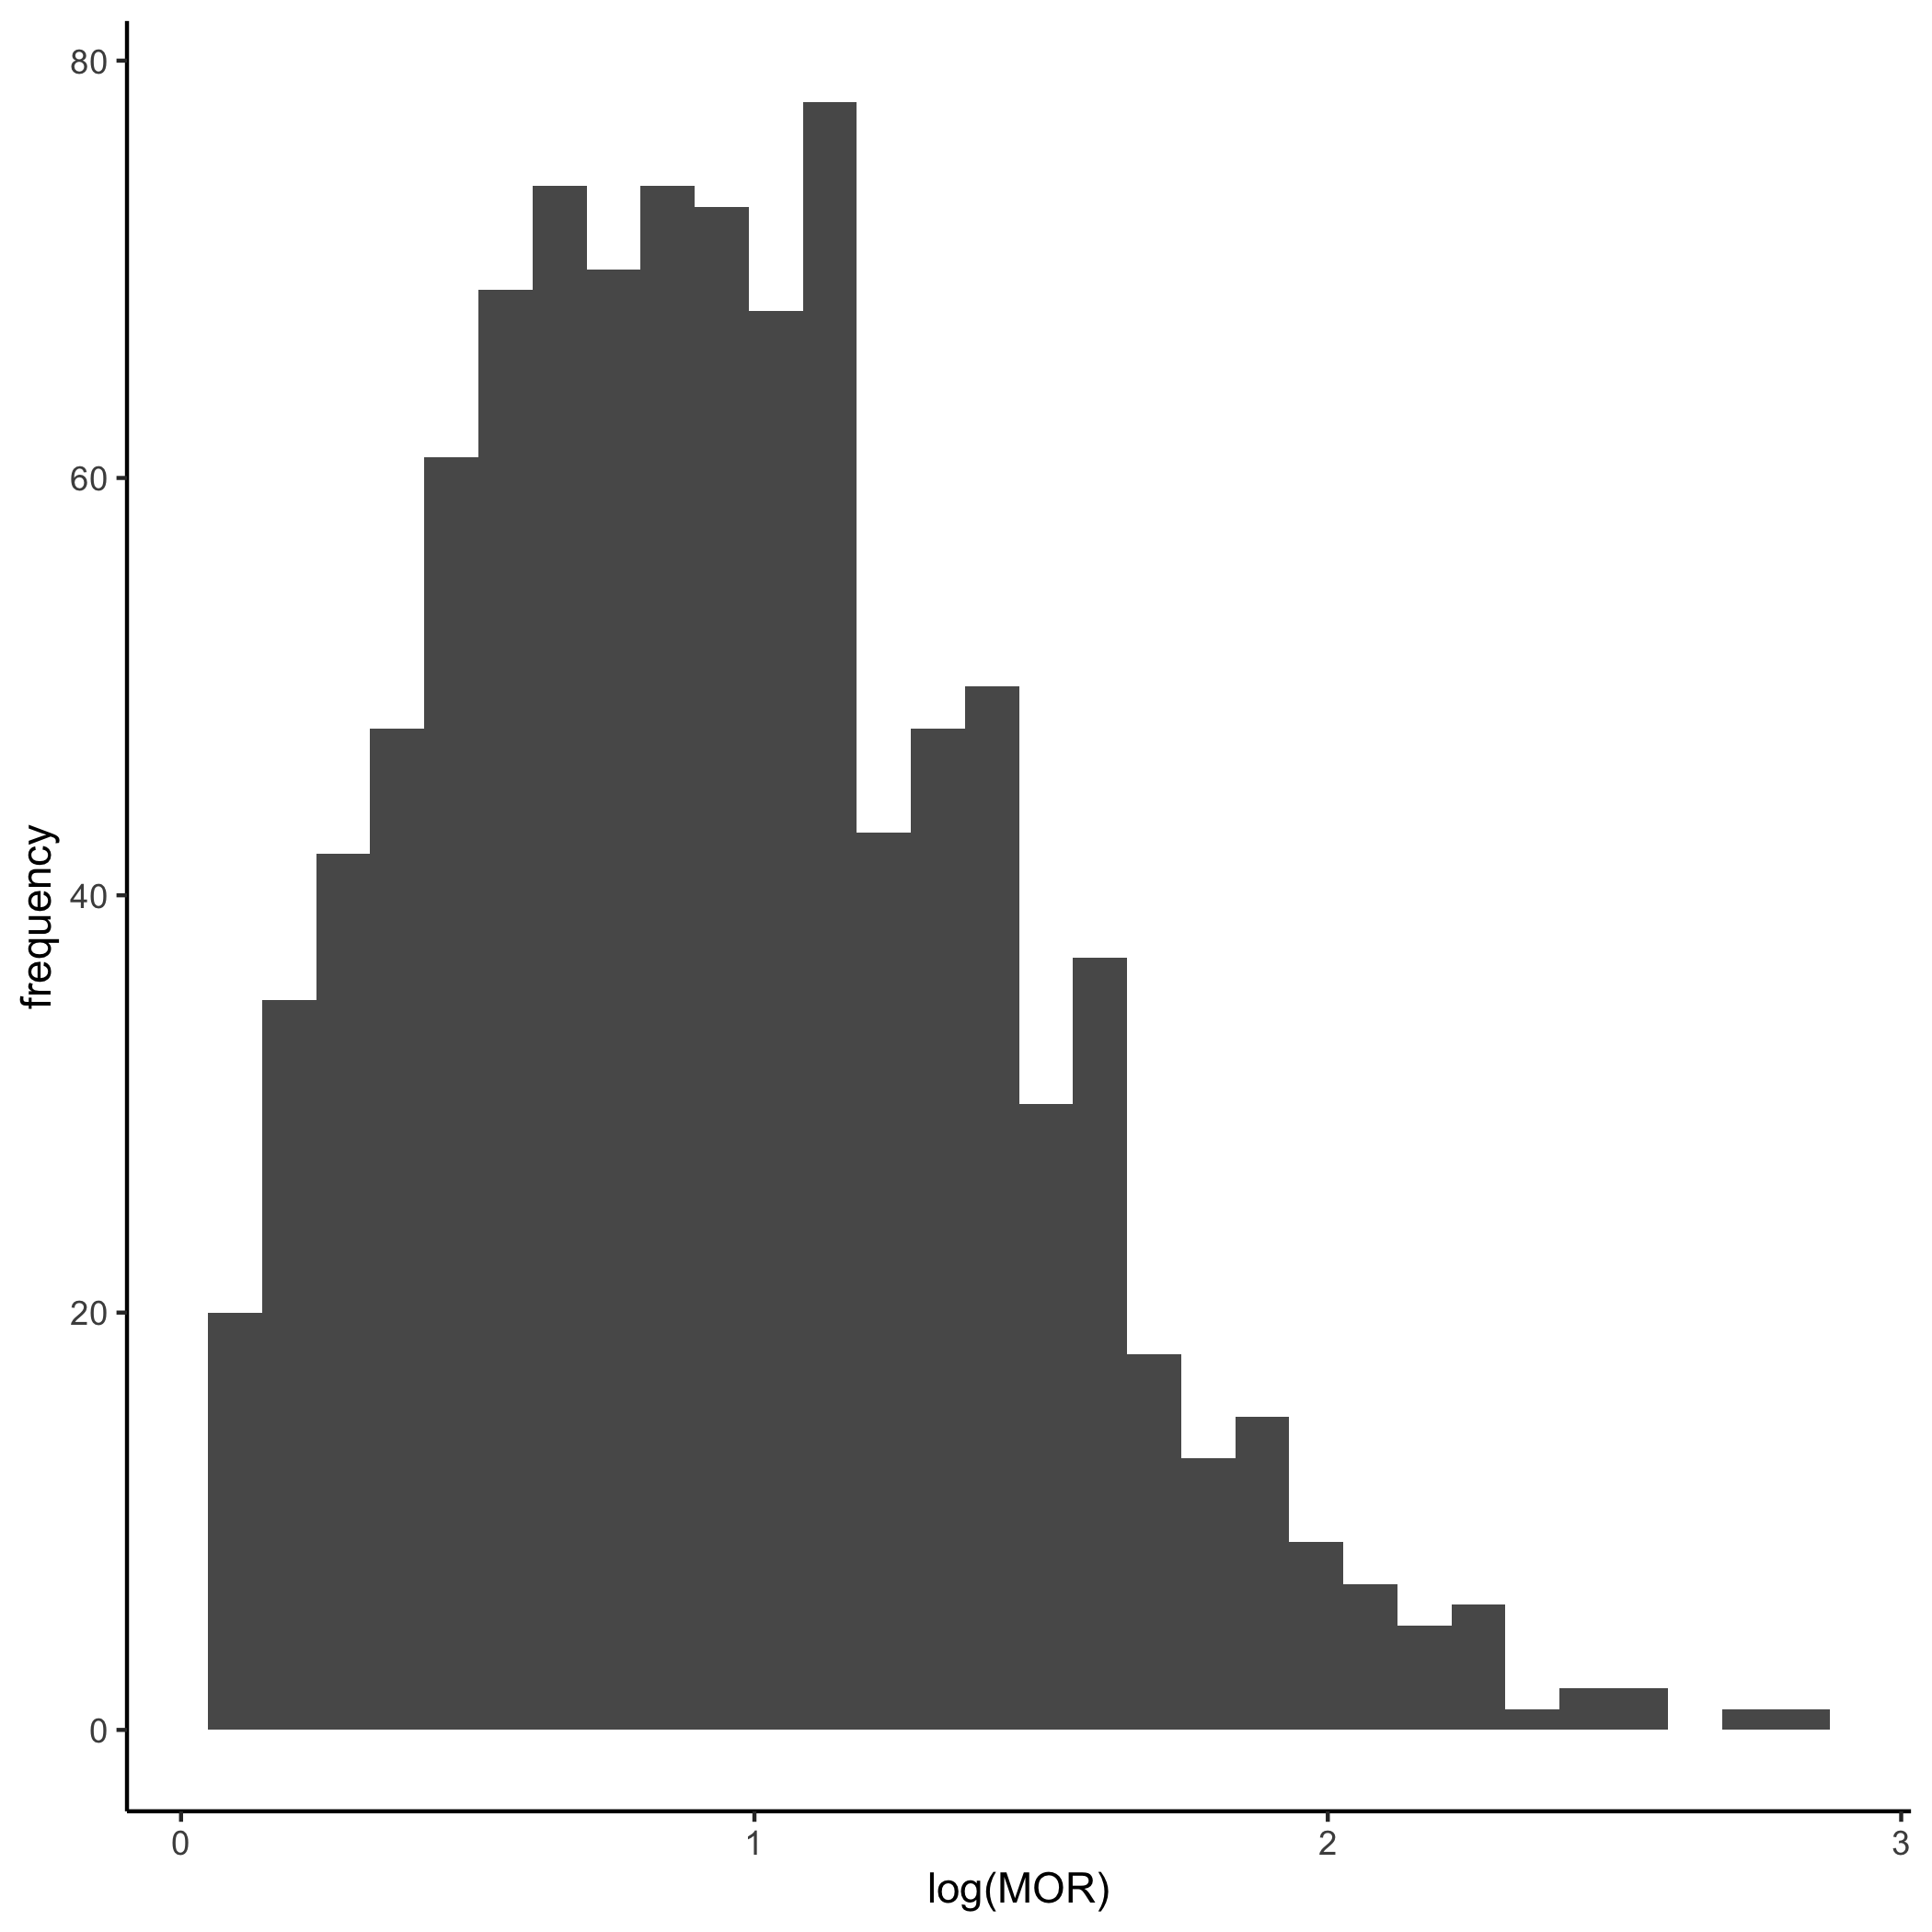
\includegraphics{../../plots/two-lvl-ran-slope/high-prev/hist_30_5_two_lvl_slp_high_prev_q2.png}

}

\caption{Cluster size 5}

}

\end{minipage}%
%
\begin{minipage}[t]{0.24\linewidth}

{\centering 

\raisebox{-\height}{

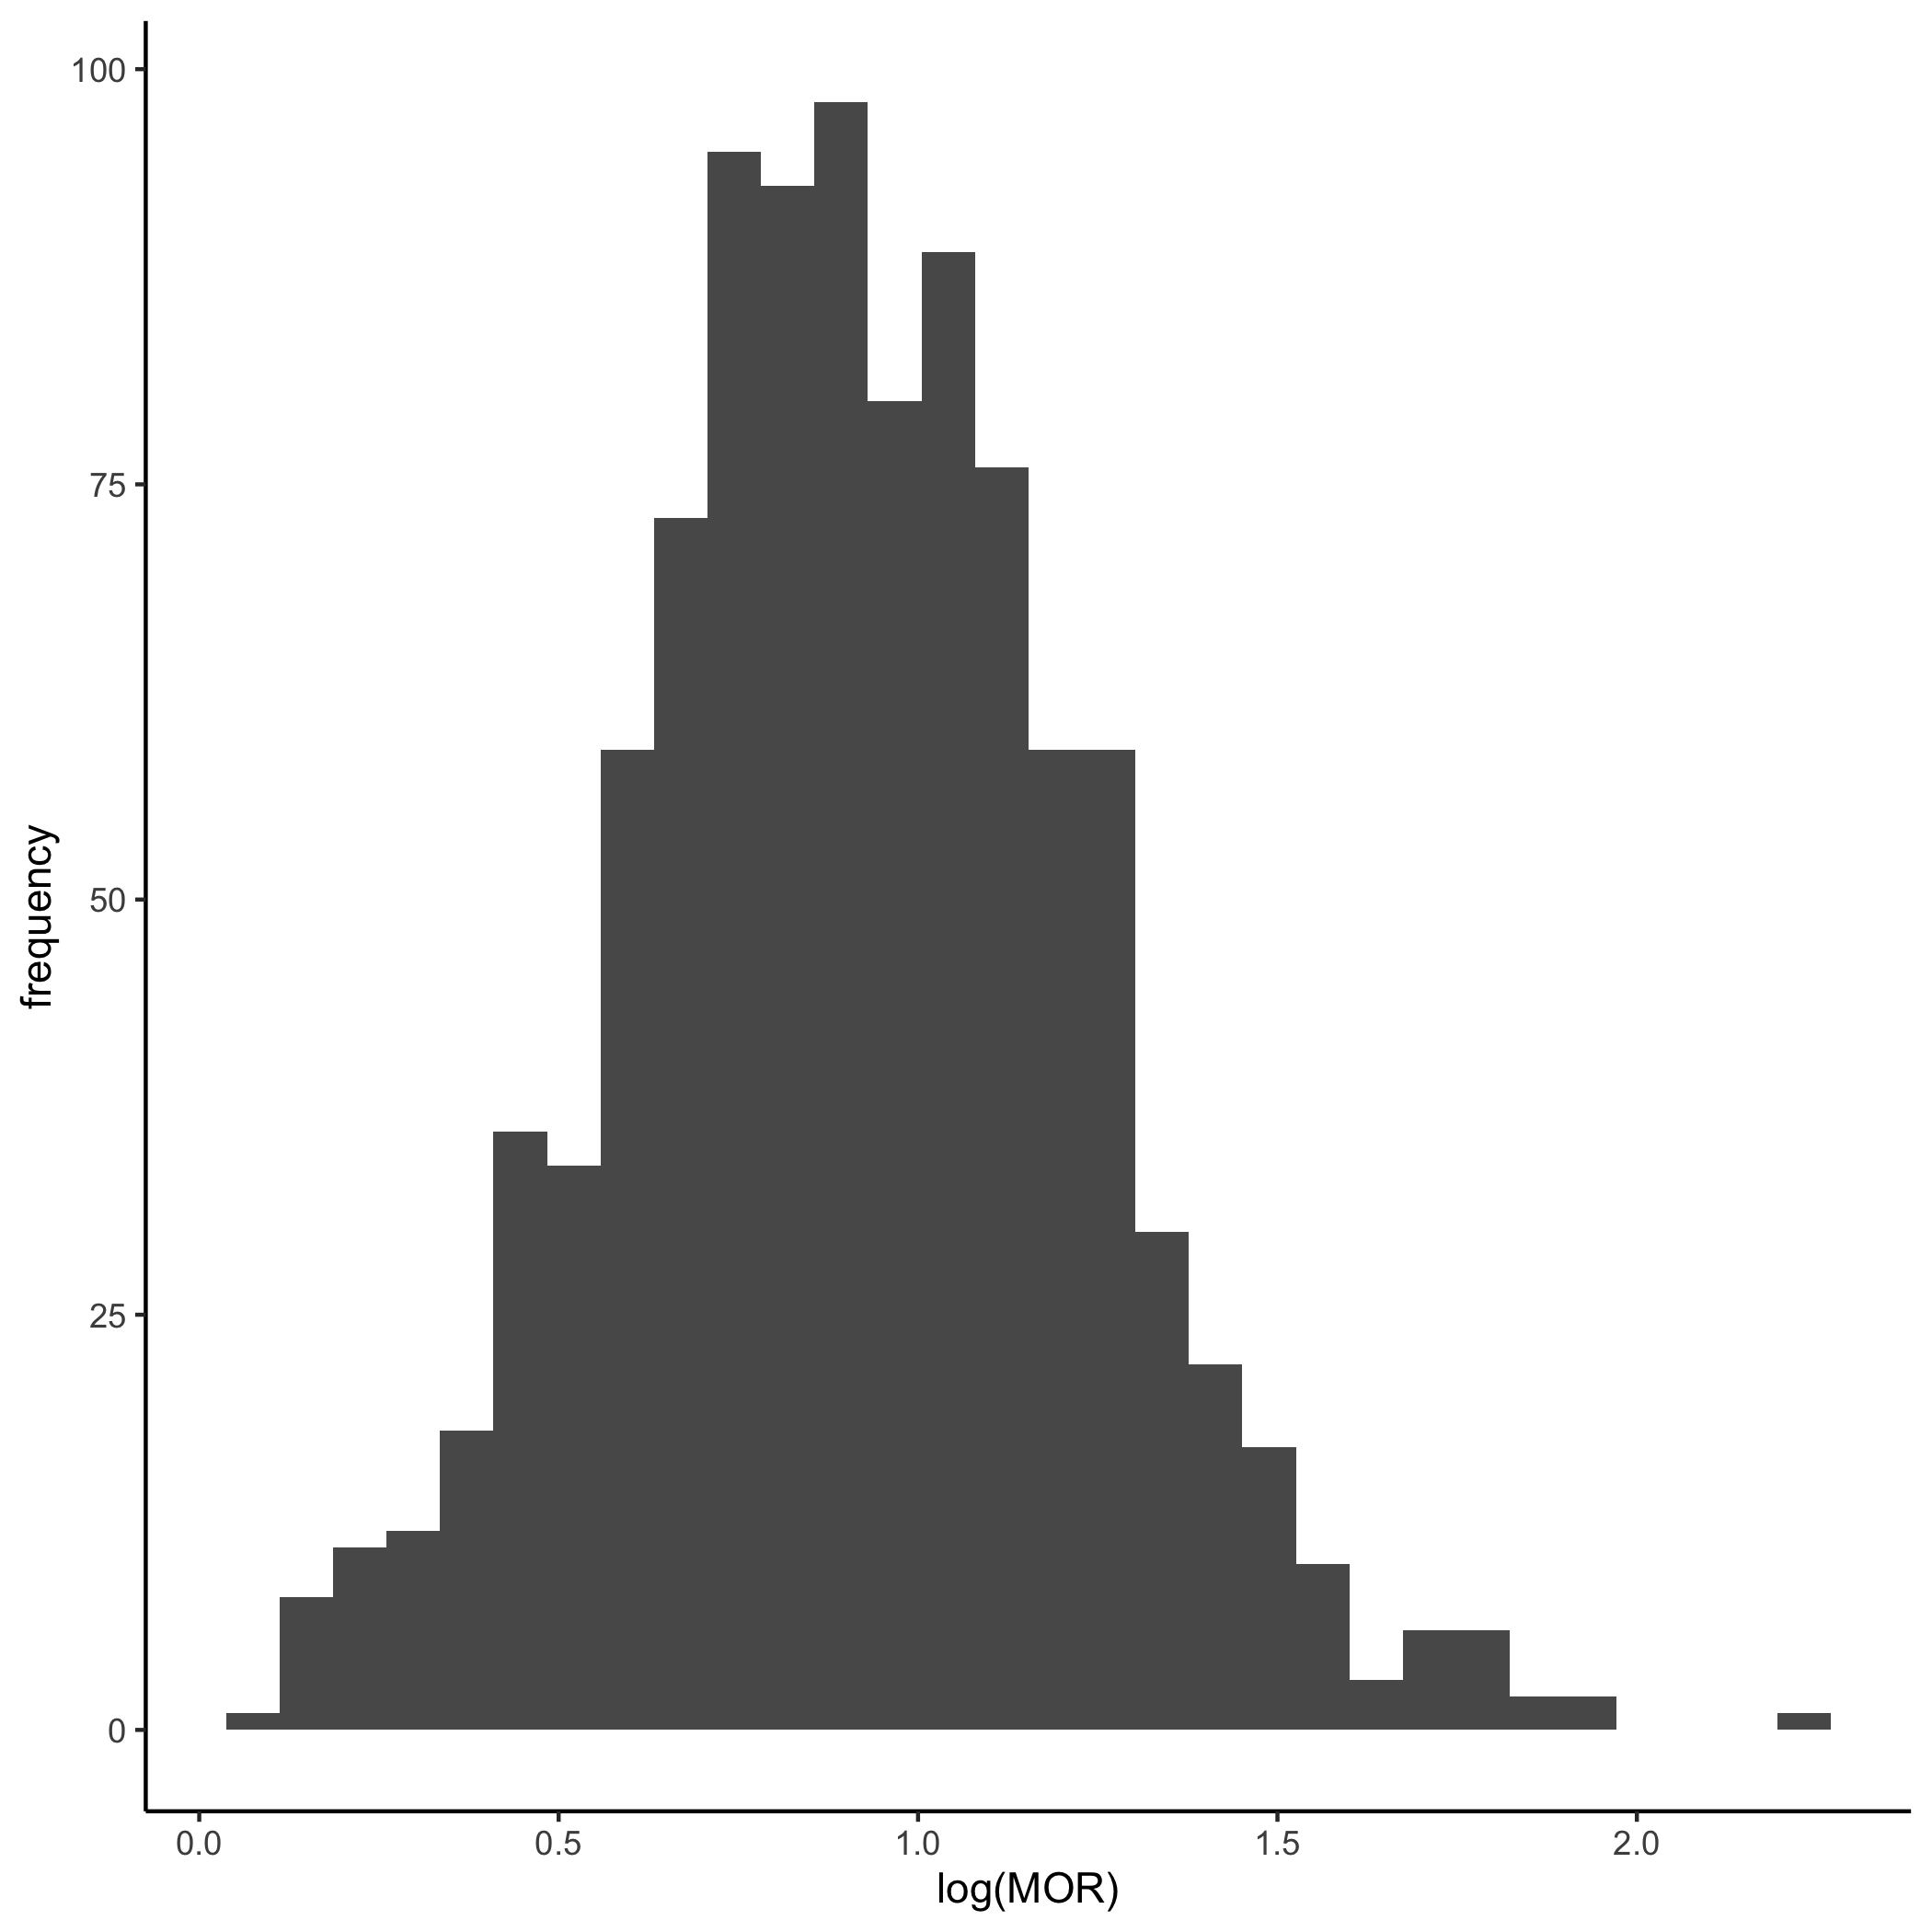
\includegraphics{../../plots/two-lvl-ran-slope/high-prev/hist_30_10_two_lvl_slp_high_prev_q2.png}

}

\caption{Cluster size 10}

}

\end{minipage}%
%
\begin{minipage}[t]{0.24\linewidth}

{\centering 

\raisebox{-\height}{

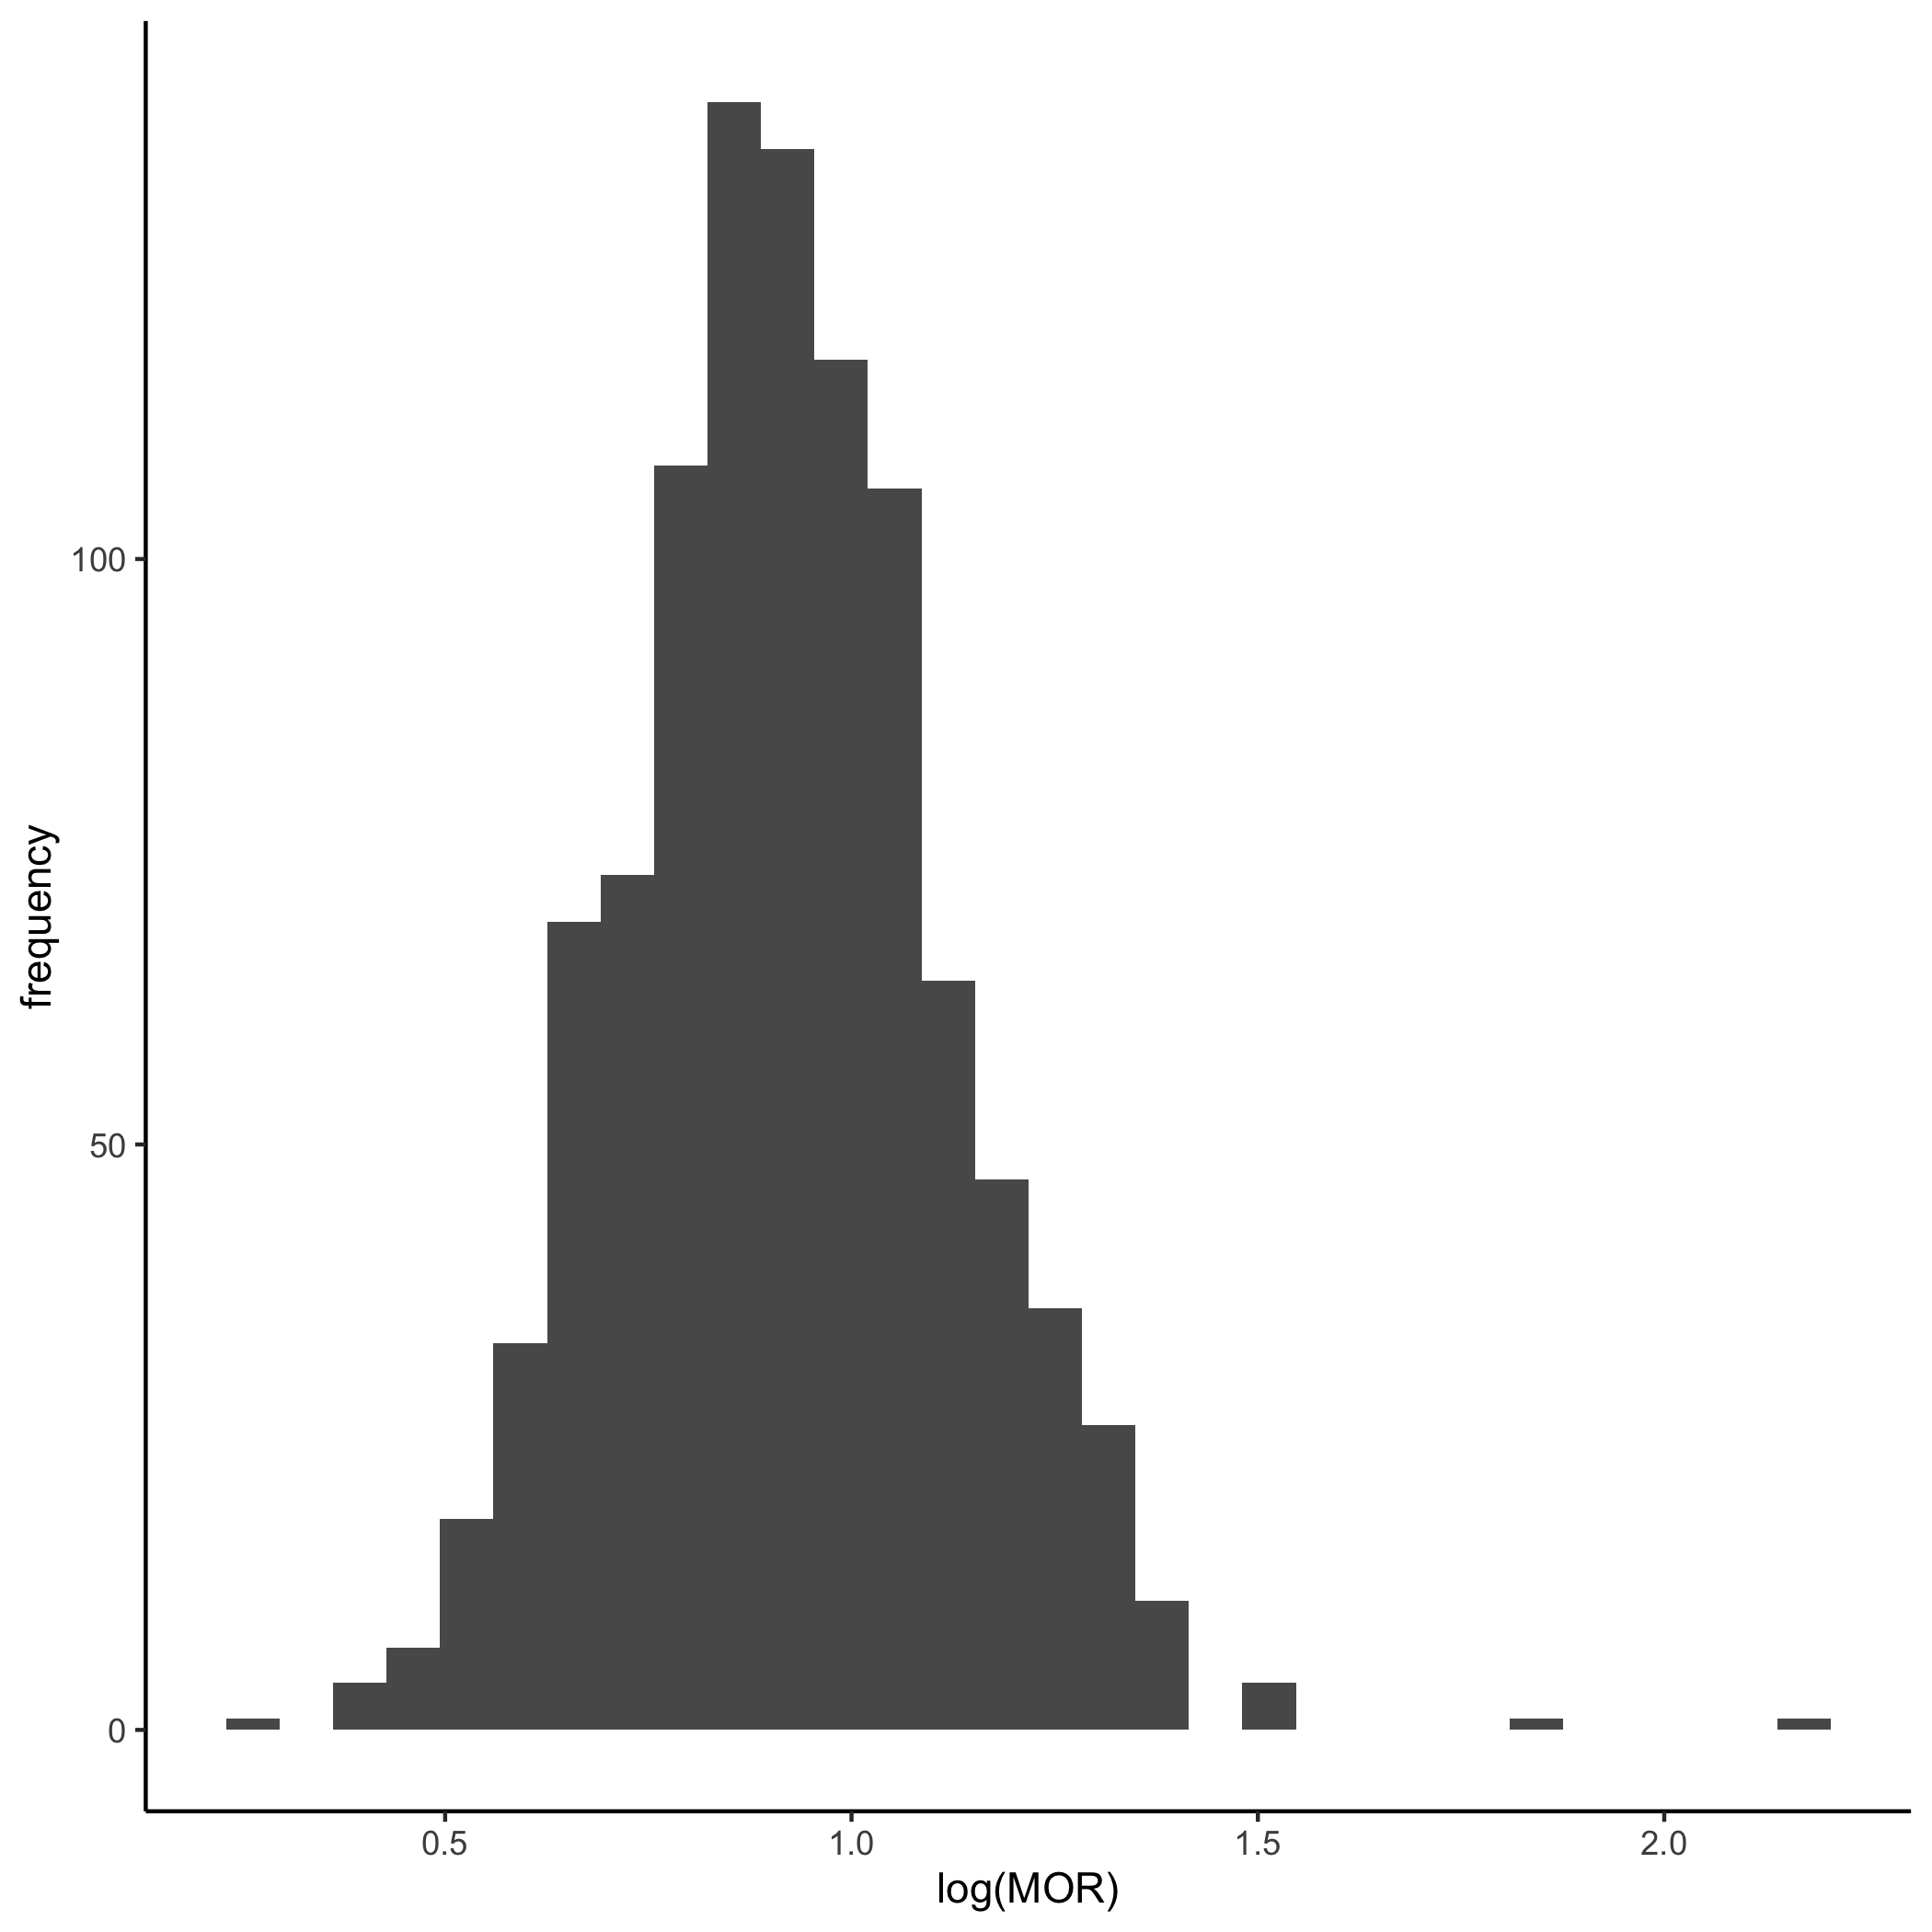
\includegraphics{../../plots/two-lvl-ran-slope/high-prev/hist_30_30_two_lvl_slp_high_prev_q2.png}

}

\caption{Cluster size 30}

}

\end{minipage}%
%
\begin{minipage}[t]{0.24\linewidth}

{\centering 

\raisebox{-\height}{

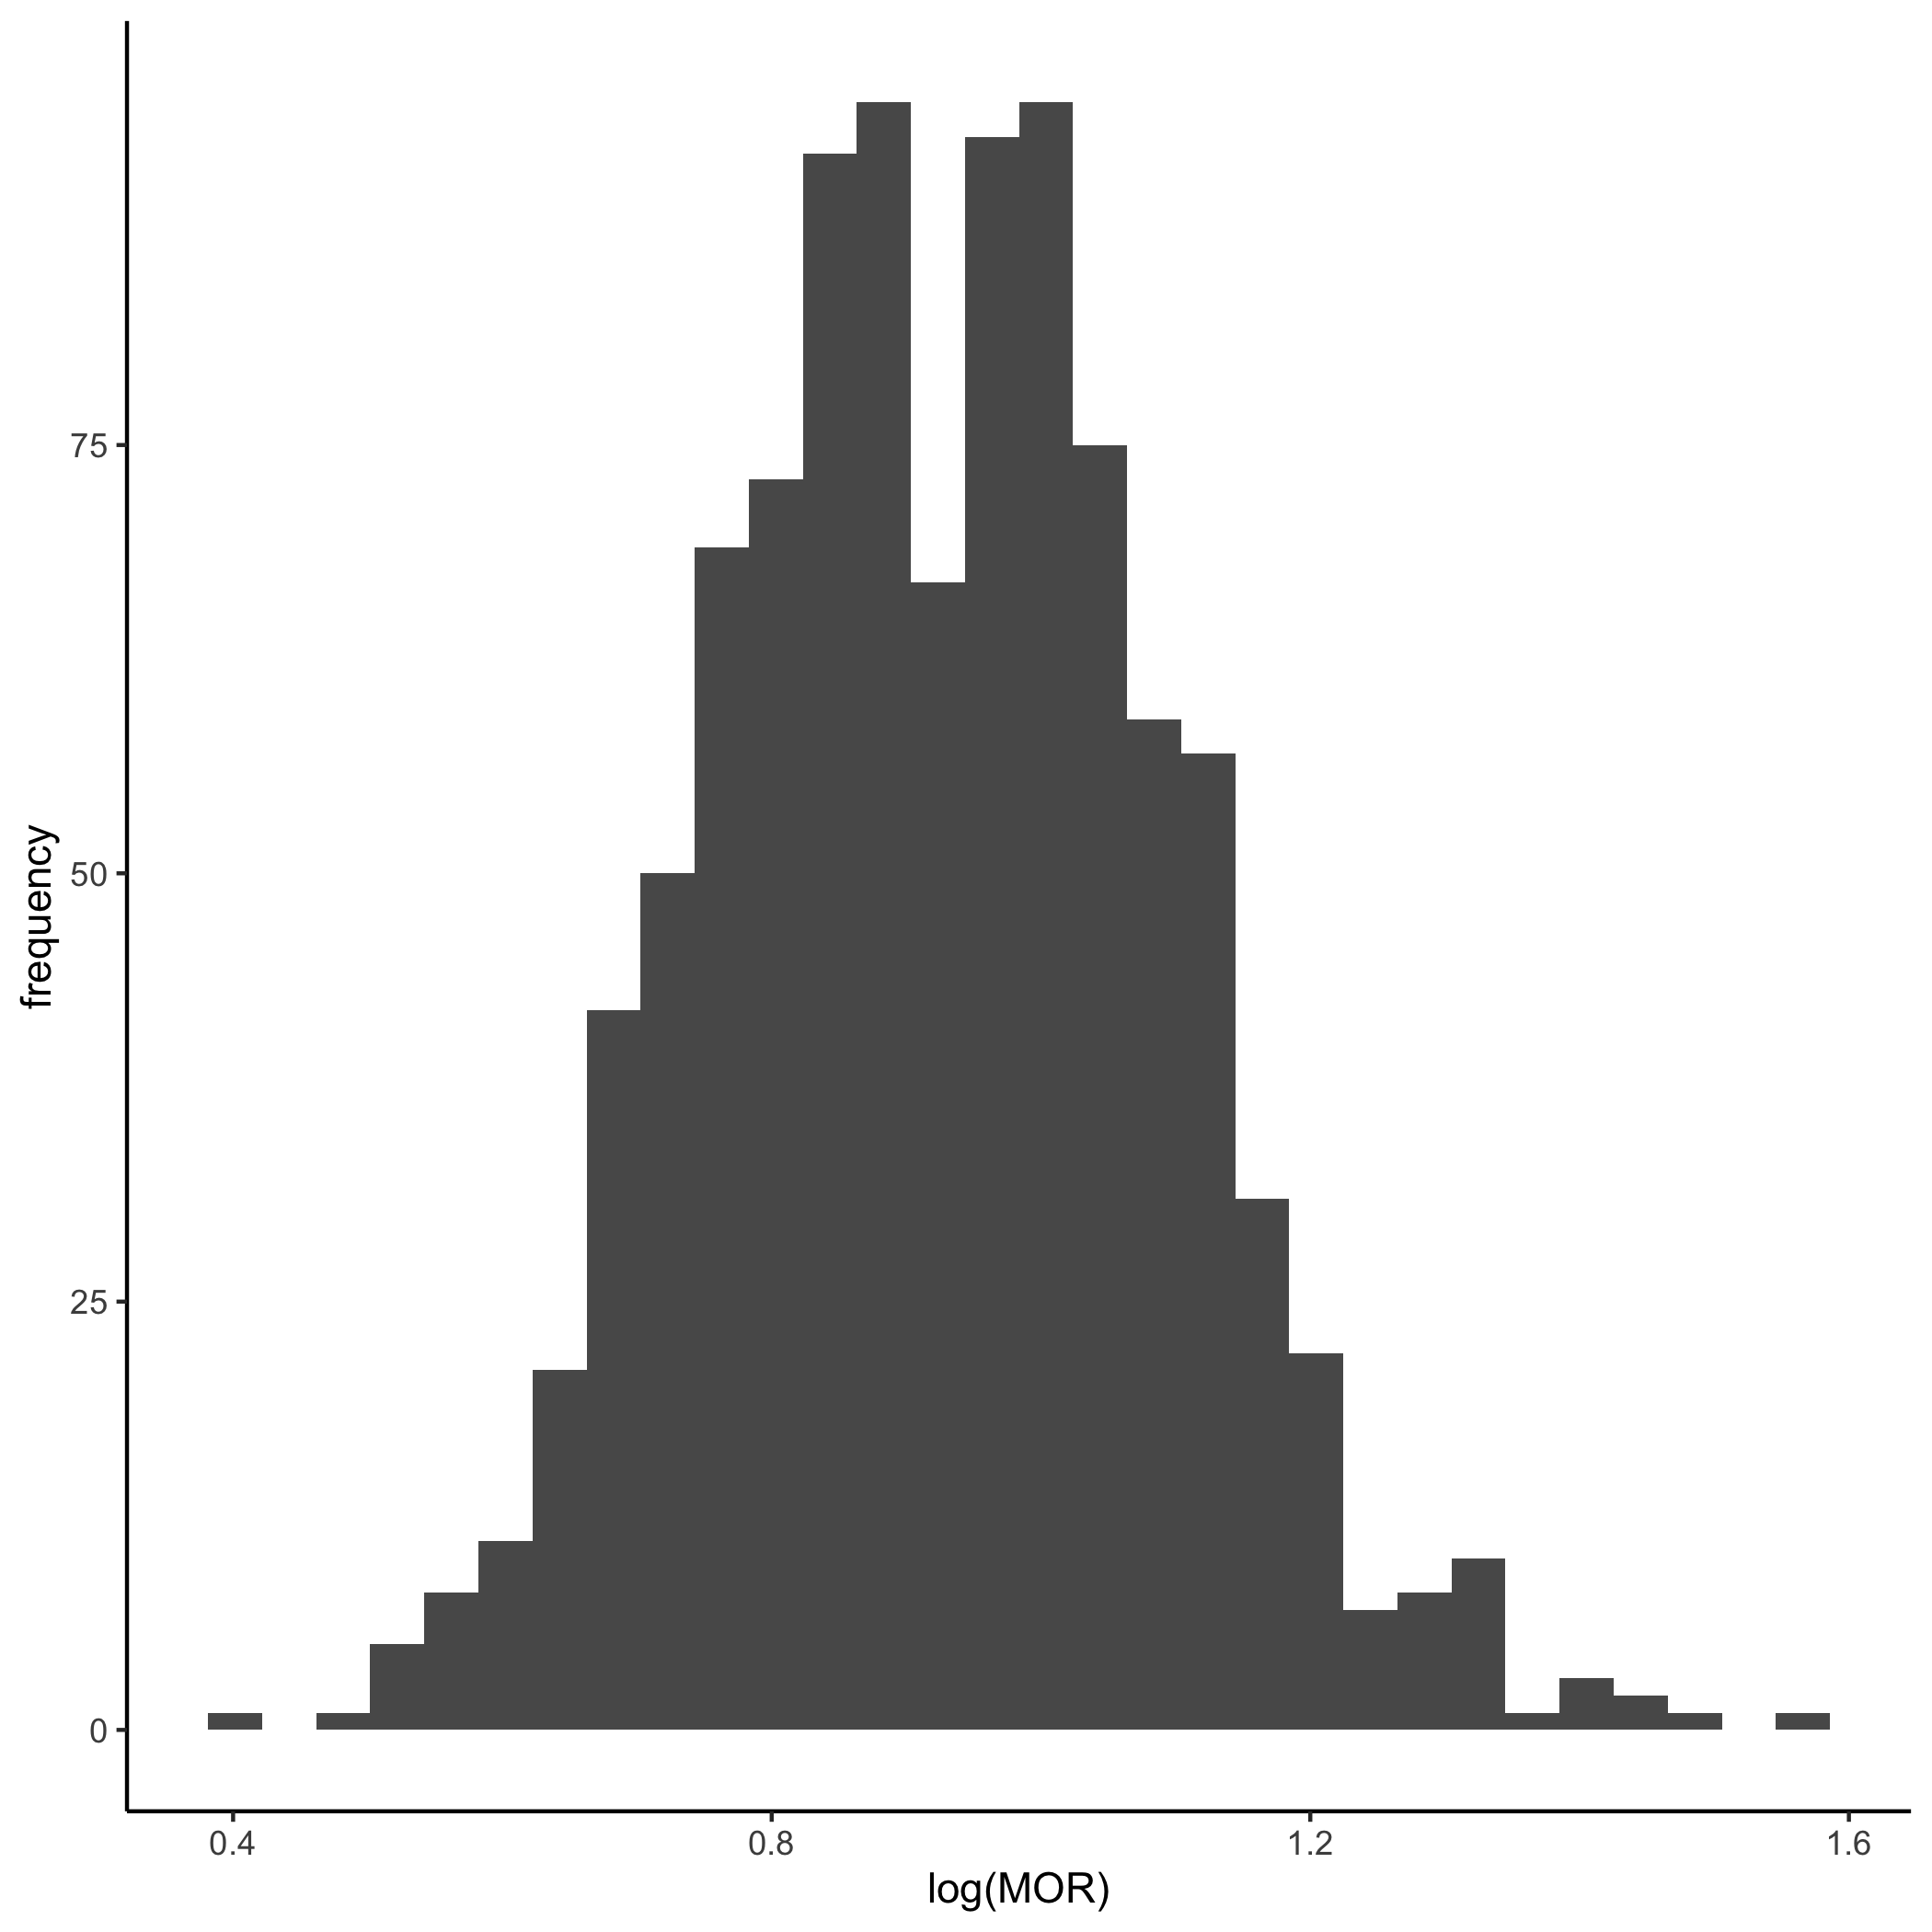
\includegraphics{../../plots/two-lvl-ran-slope/high-prev/hist_30_50_two_lvl_slp_high_prev_q2.png}

}

\caption{Cluster size 50}

}

\end{minipage}%
\newline
\begin{minipage}[t]{\linewidth}

{\centering 

~

}

\end{minipage}%
\newline
\begin{minipage}[t]{0.05\linewidth}

{\centering 

\rotatebox[origin=br]{90}{\tiny Cluster Number 50}

}

\end{minipage}%
%
\begin{minipage}[t]{0.24\linewidth}

{\centering 

\raisebox{-\height}{

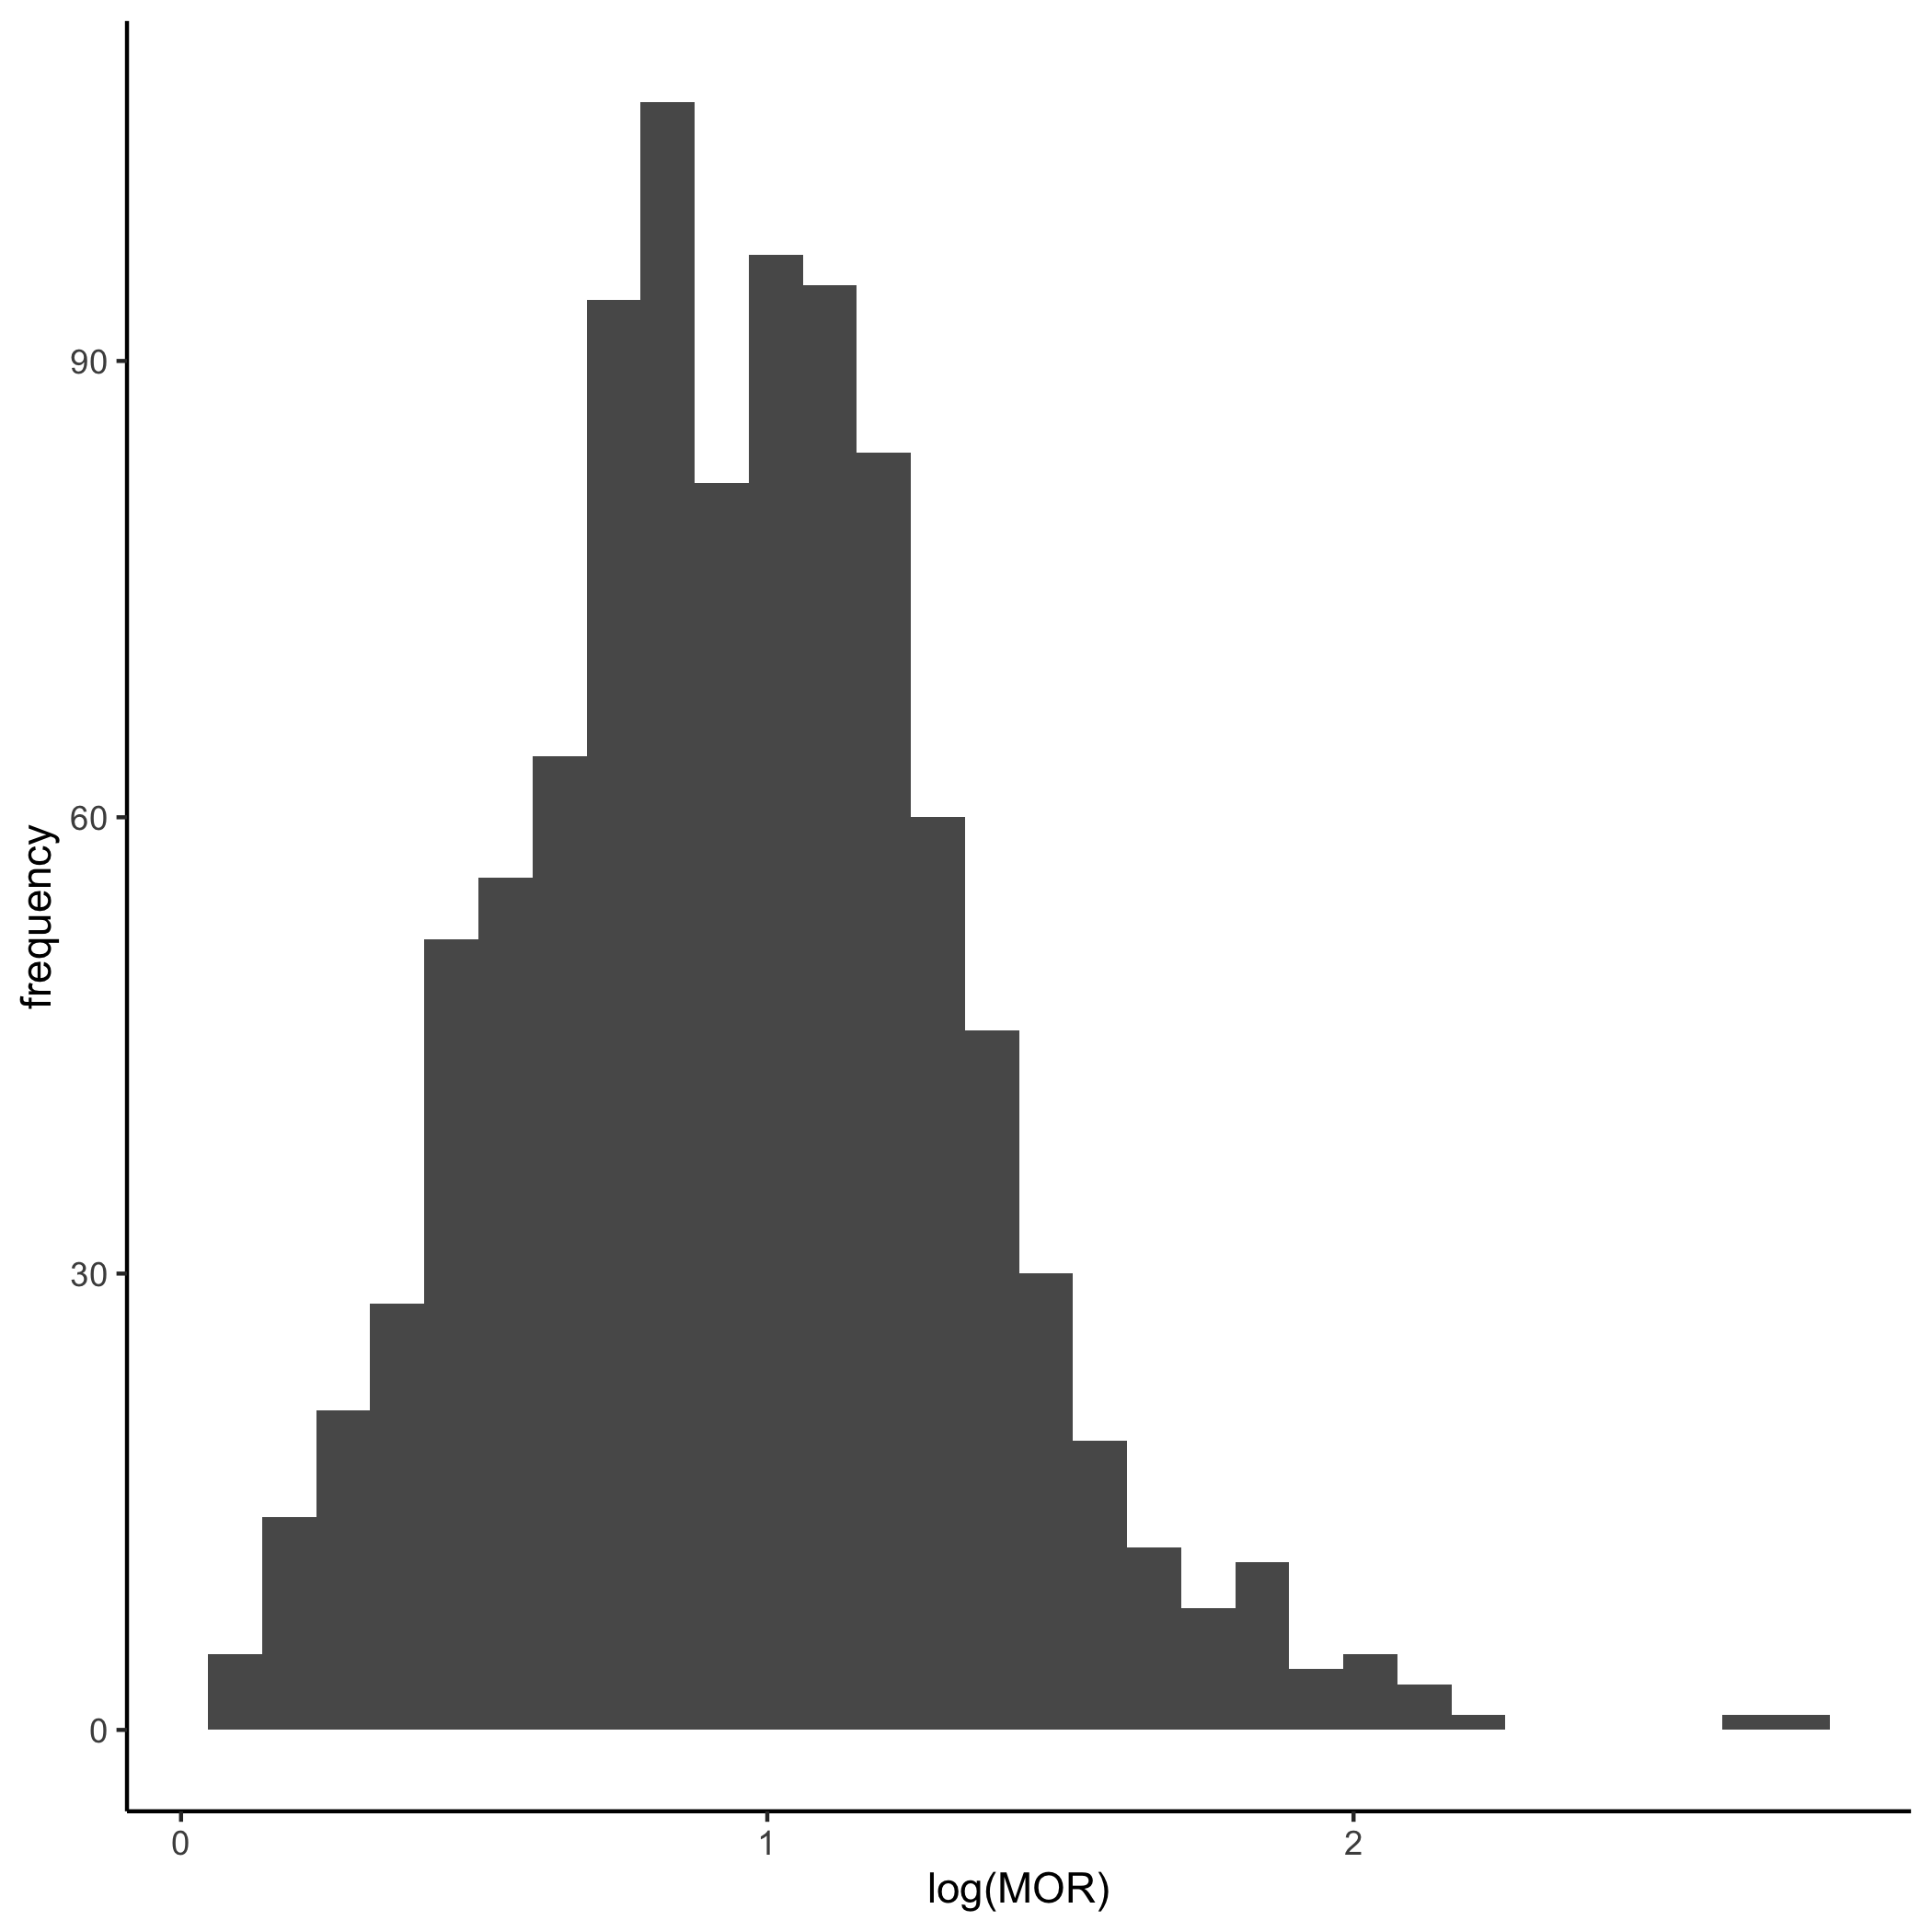
\includegraphics{../../plots/two-lvl-ran-slope/high-prev/hist_50_5_two_lvl_slp_high_prev_q2.png}

}

\caption{Cluster size 5}

}

\end{minipage}%
%
\begin{minipage}[t]{0.24\linewidth}

{\centering 

\raisebox{-\height}{

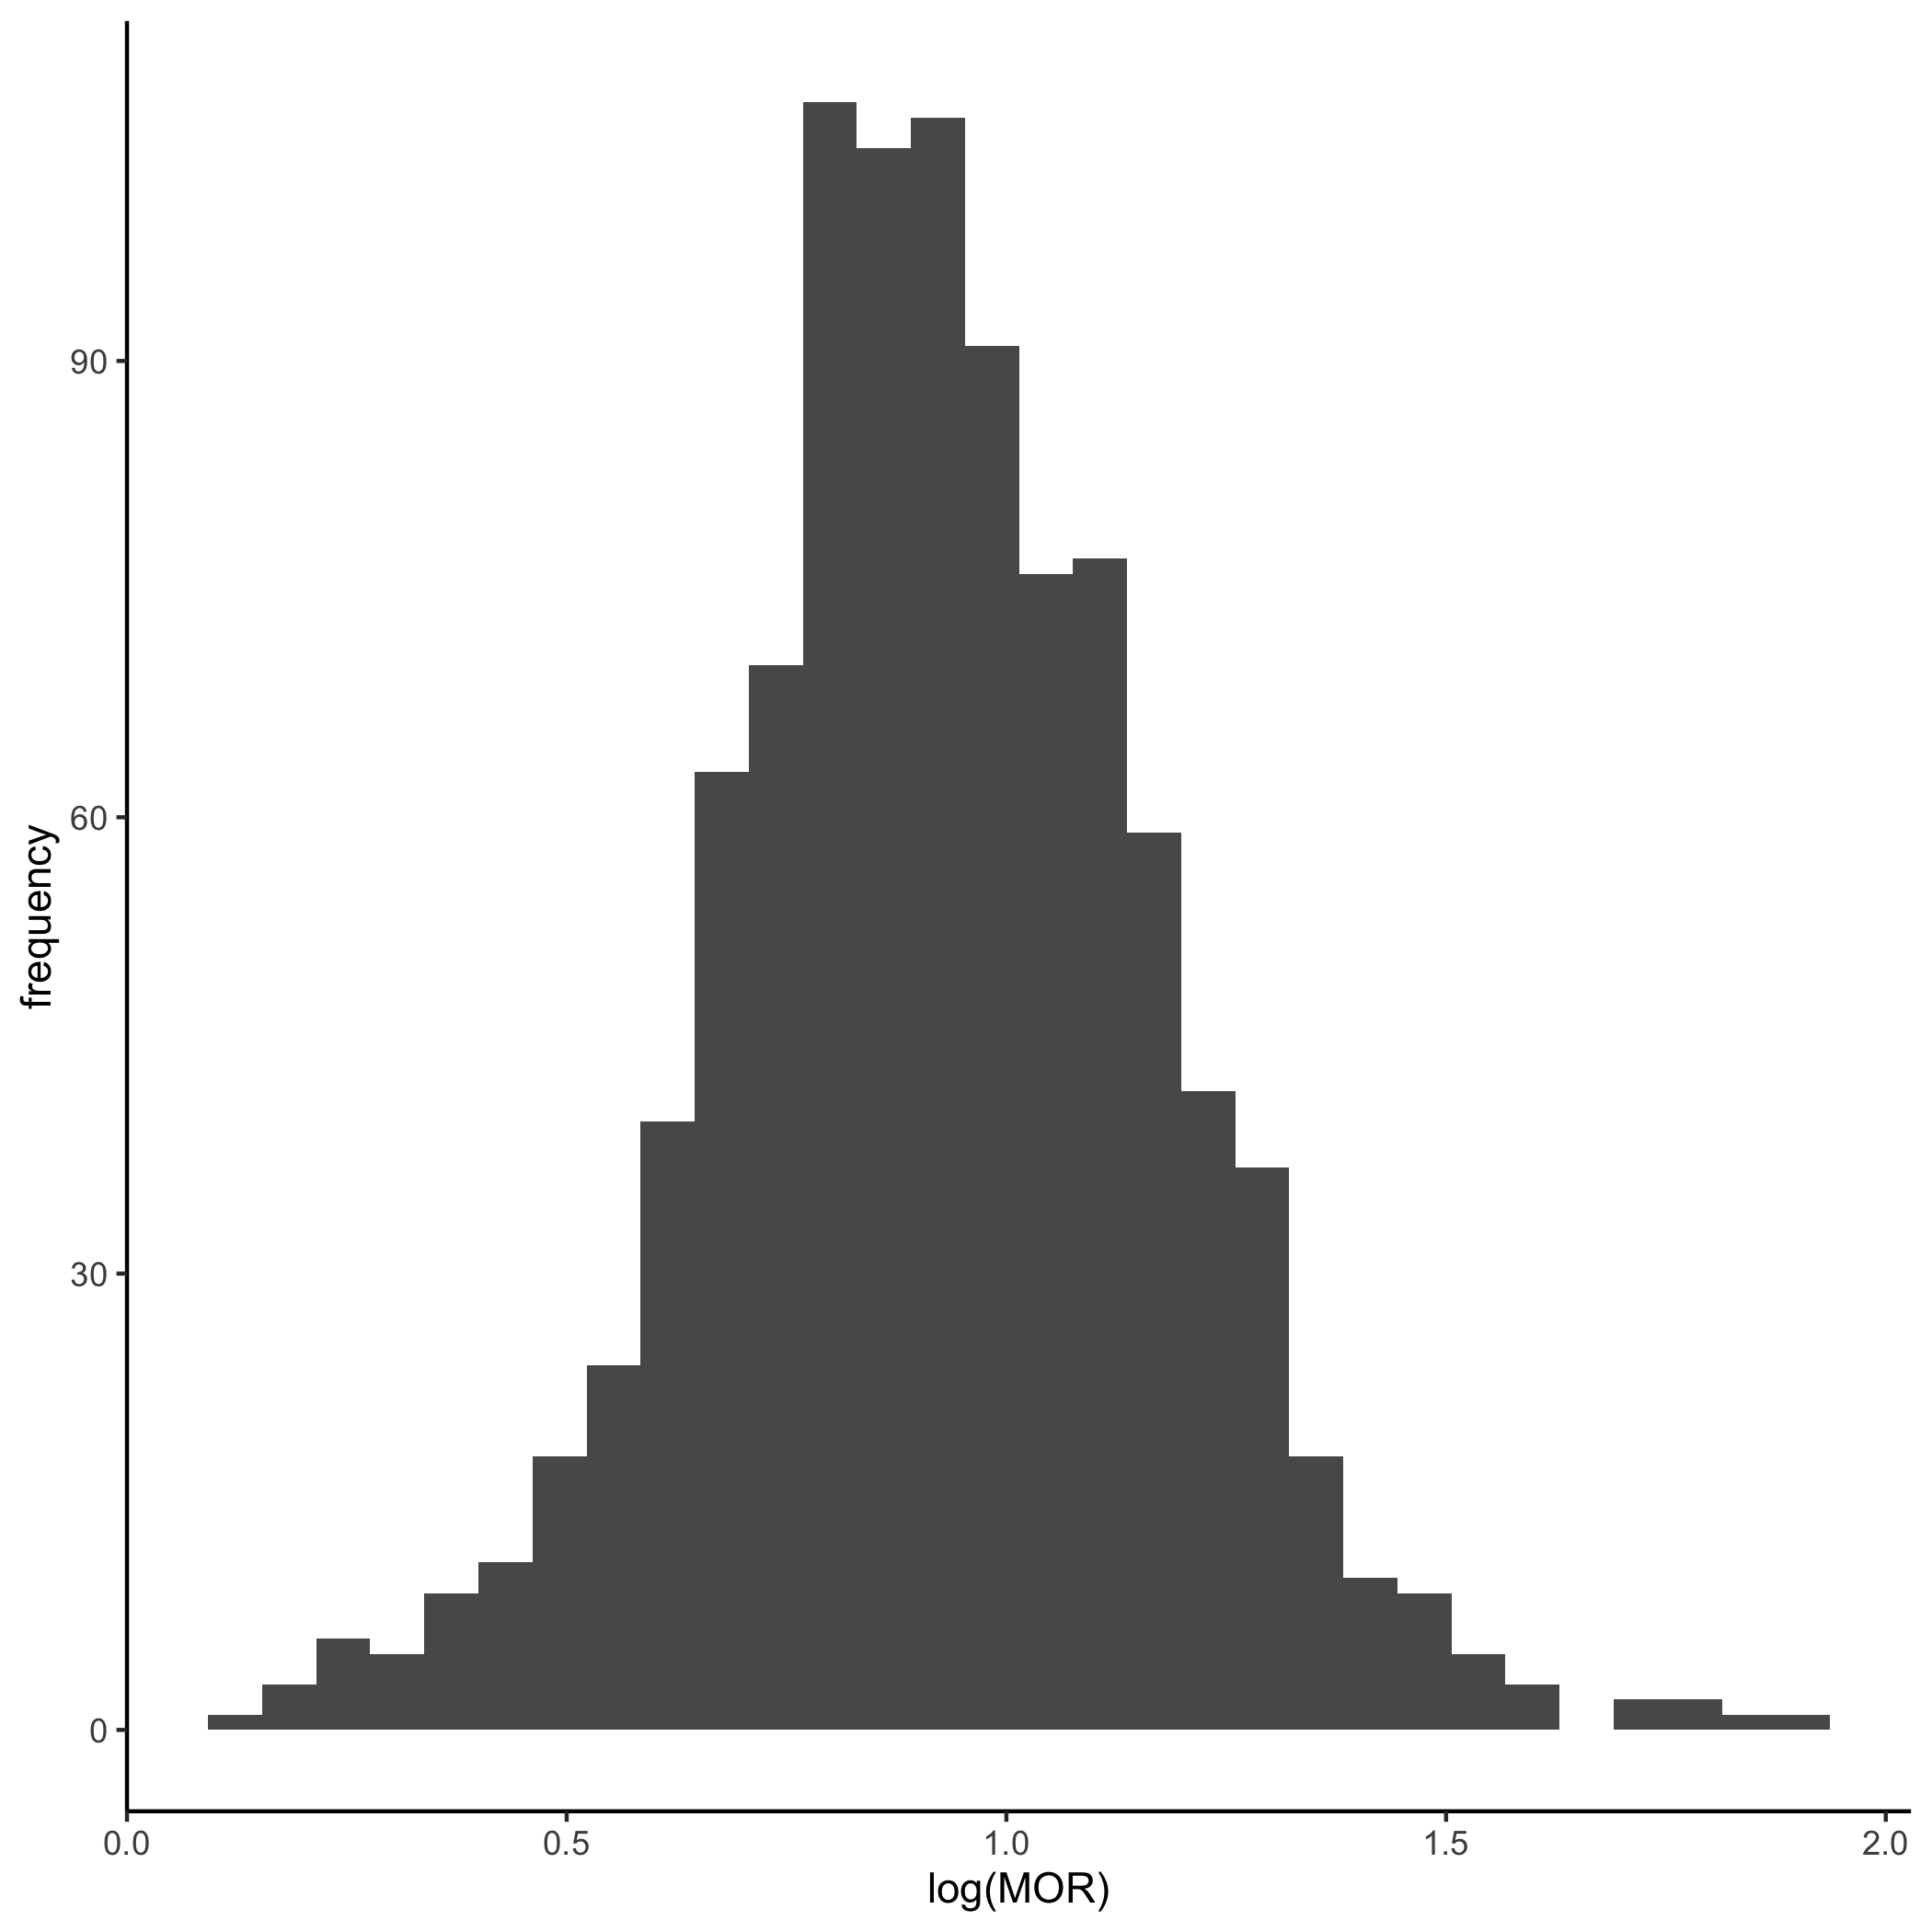
\includegraphics{../../plots/two-lvl-ran-slope/high-prev/hist_50_10_two_lvl_slp_high_prev_q2.png}

}

\caption{Cluster size 10}

}

\end{minipage}%
%
\begin{minipage}[t]{0.24\linewidth}

{\centering 

\raisebox{-\height}{

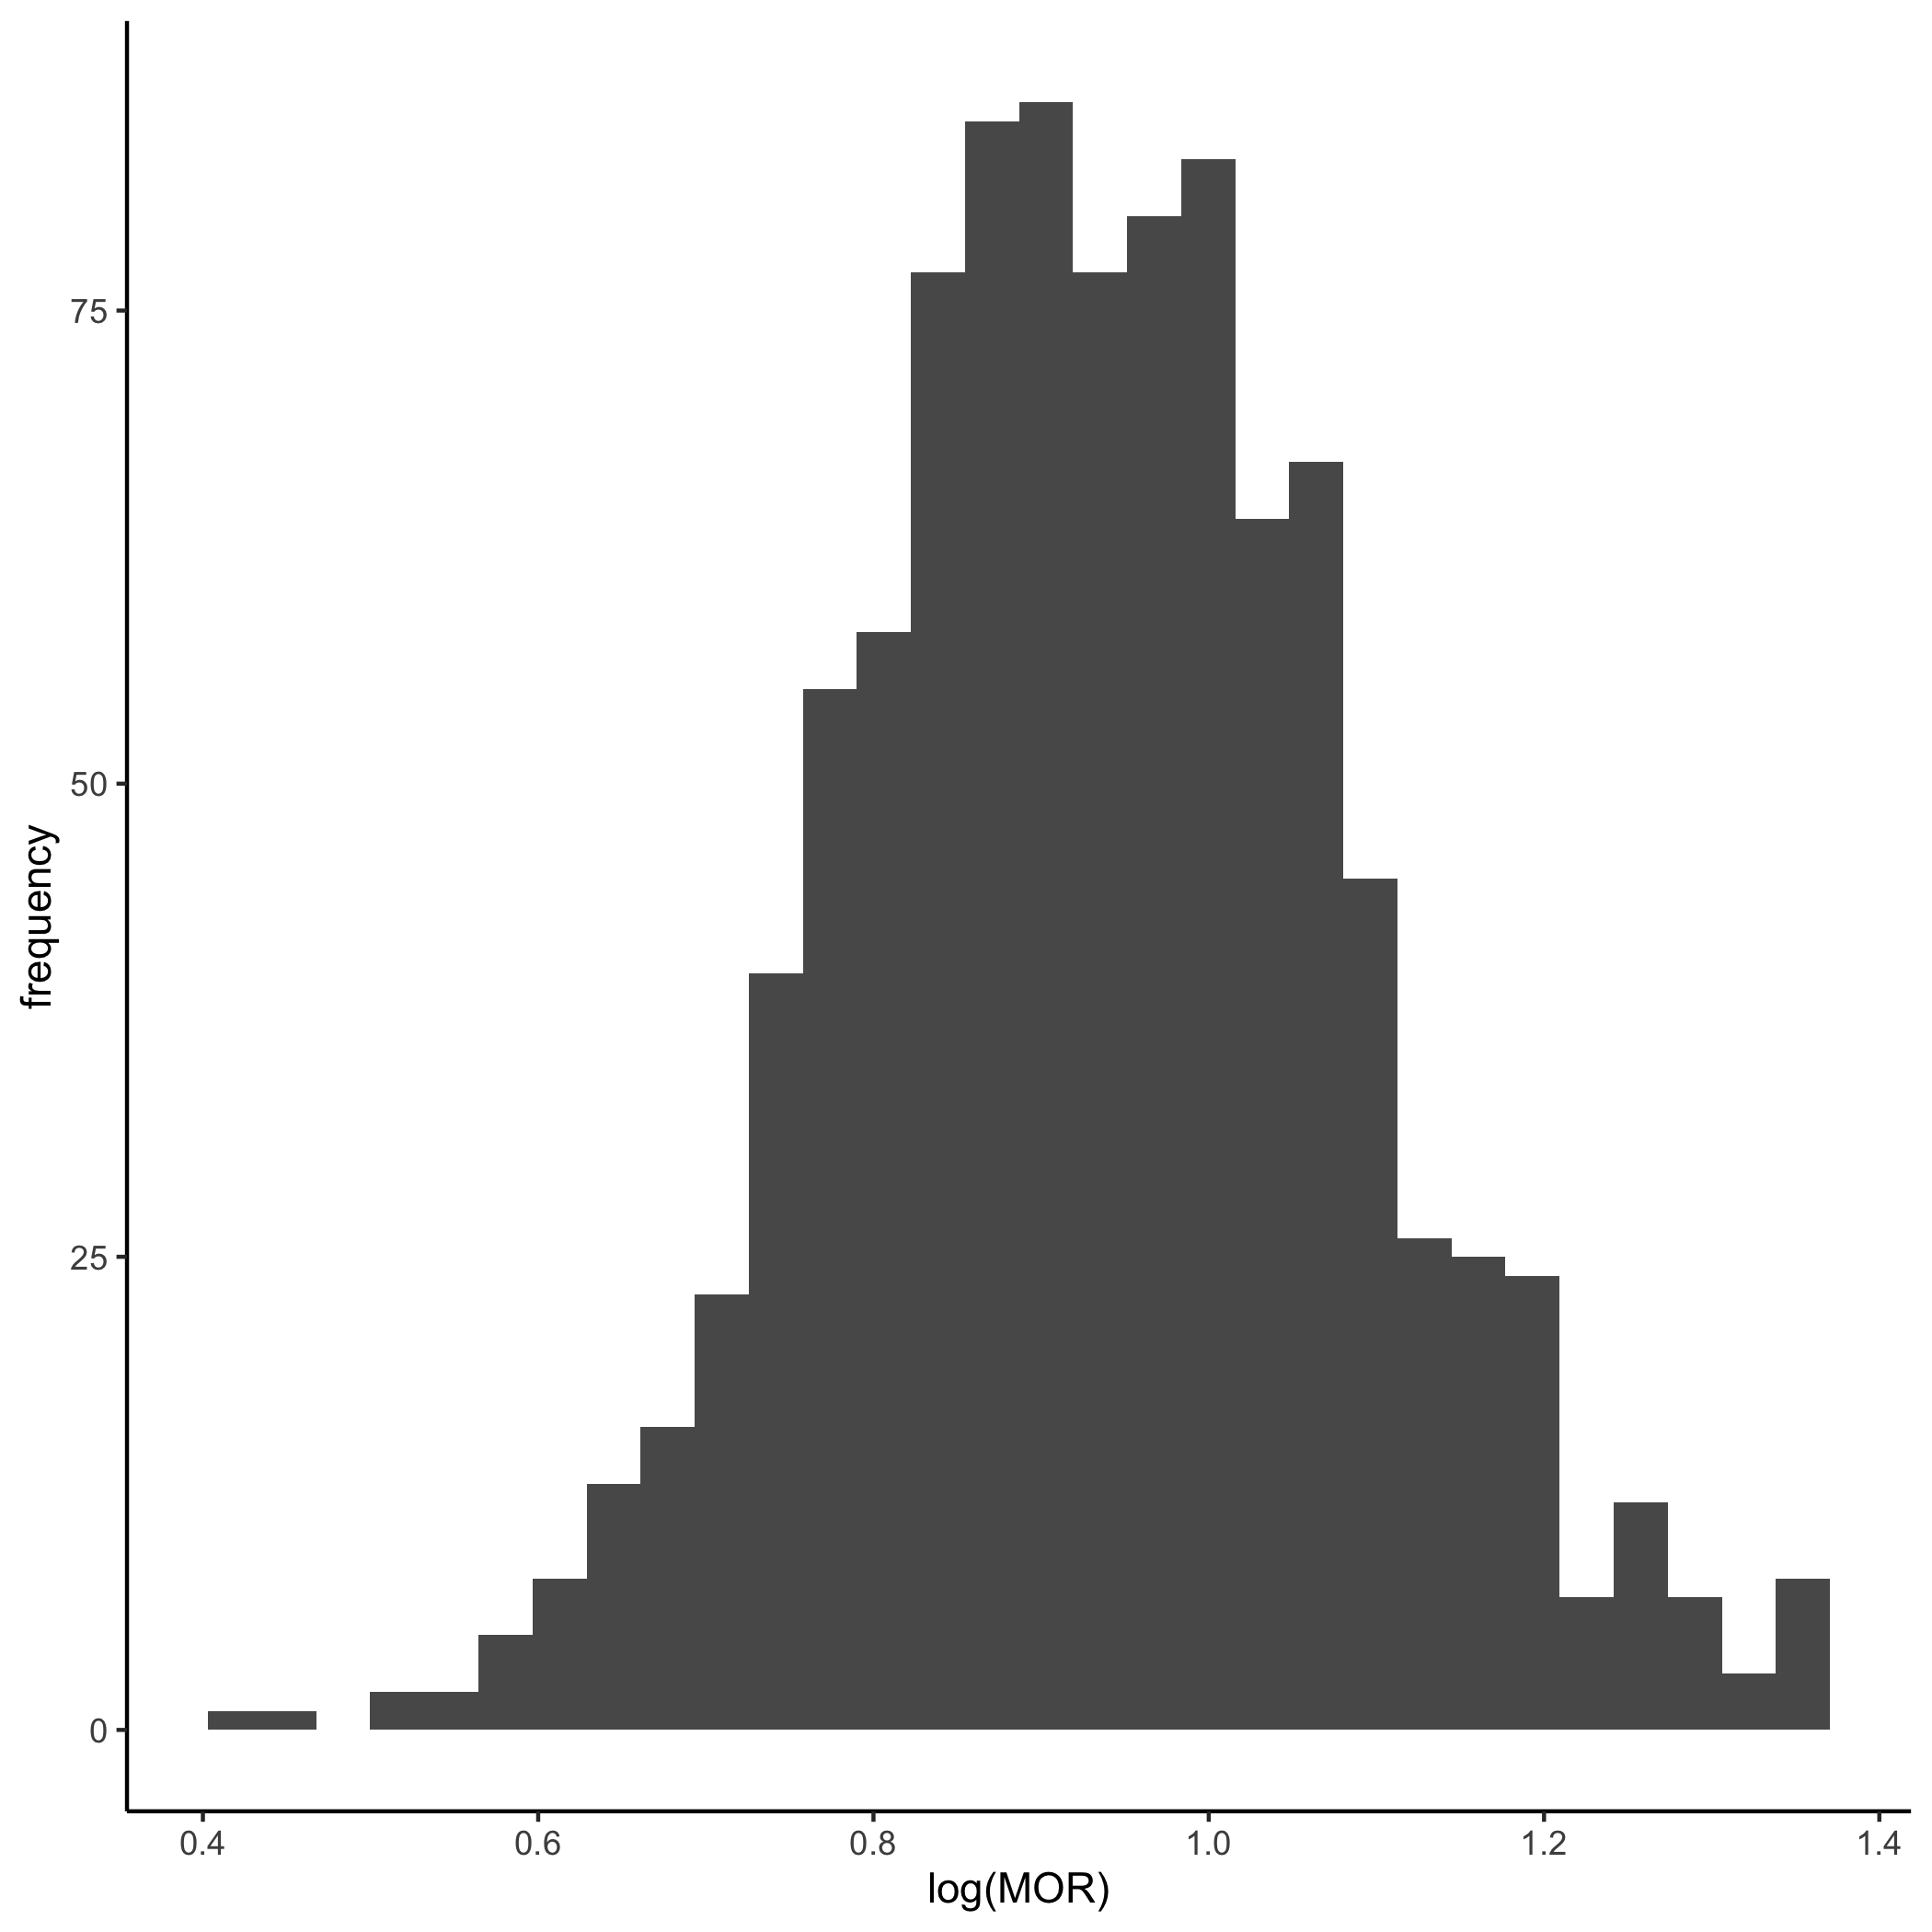
\includegraphics{../../plots/two-lvl-ran-slope/high-prev/hist_50_30_two_lvl_slp_high_prev_q2.png}

}

\caption{Cluster size 30}

}

\end{minipage}%
%
\begin{minipage}[t]{0.24\linewidth}

{\centering 

\raisebox{-\height}{

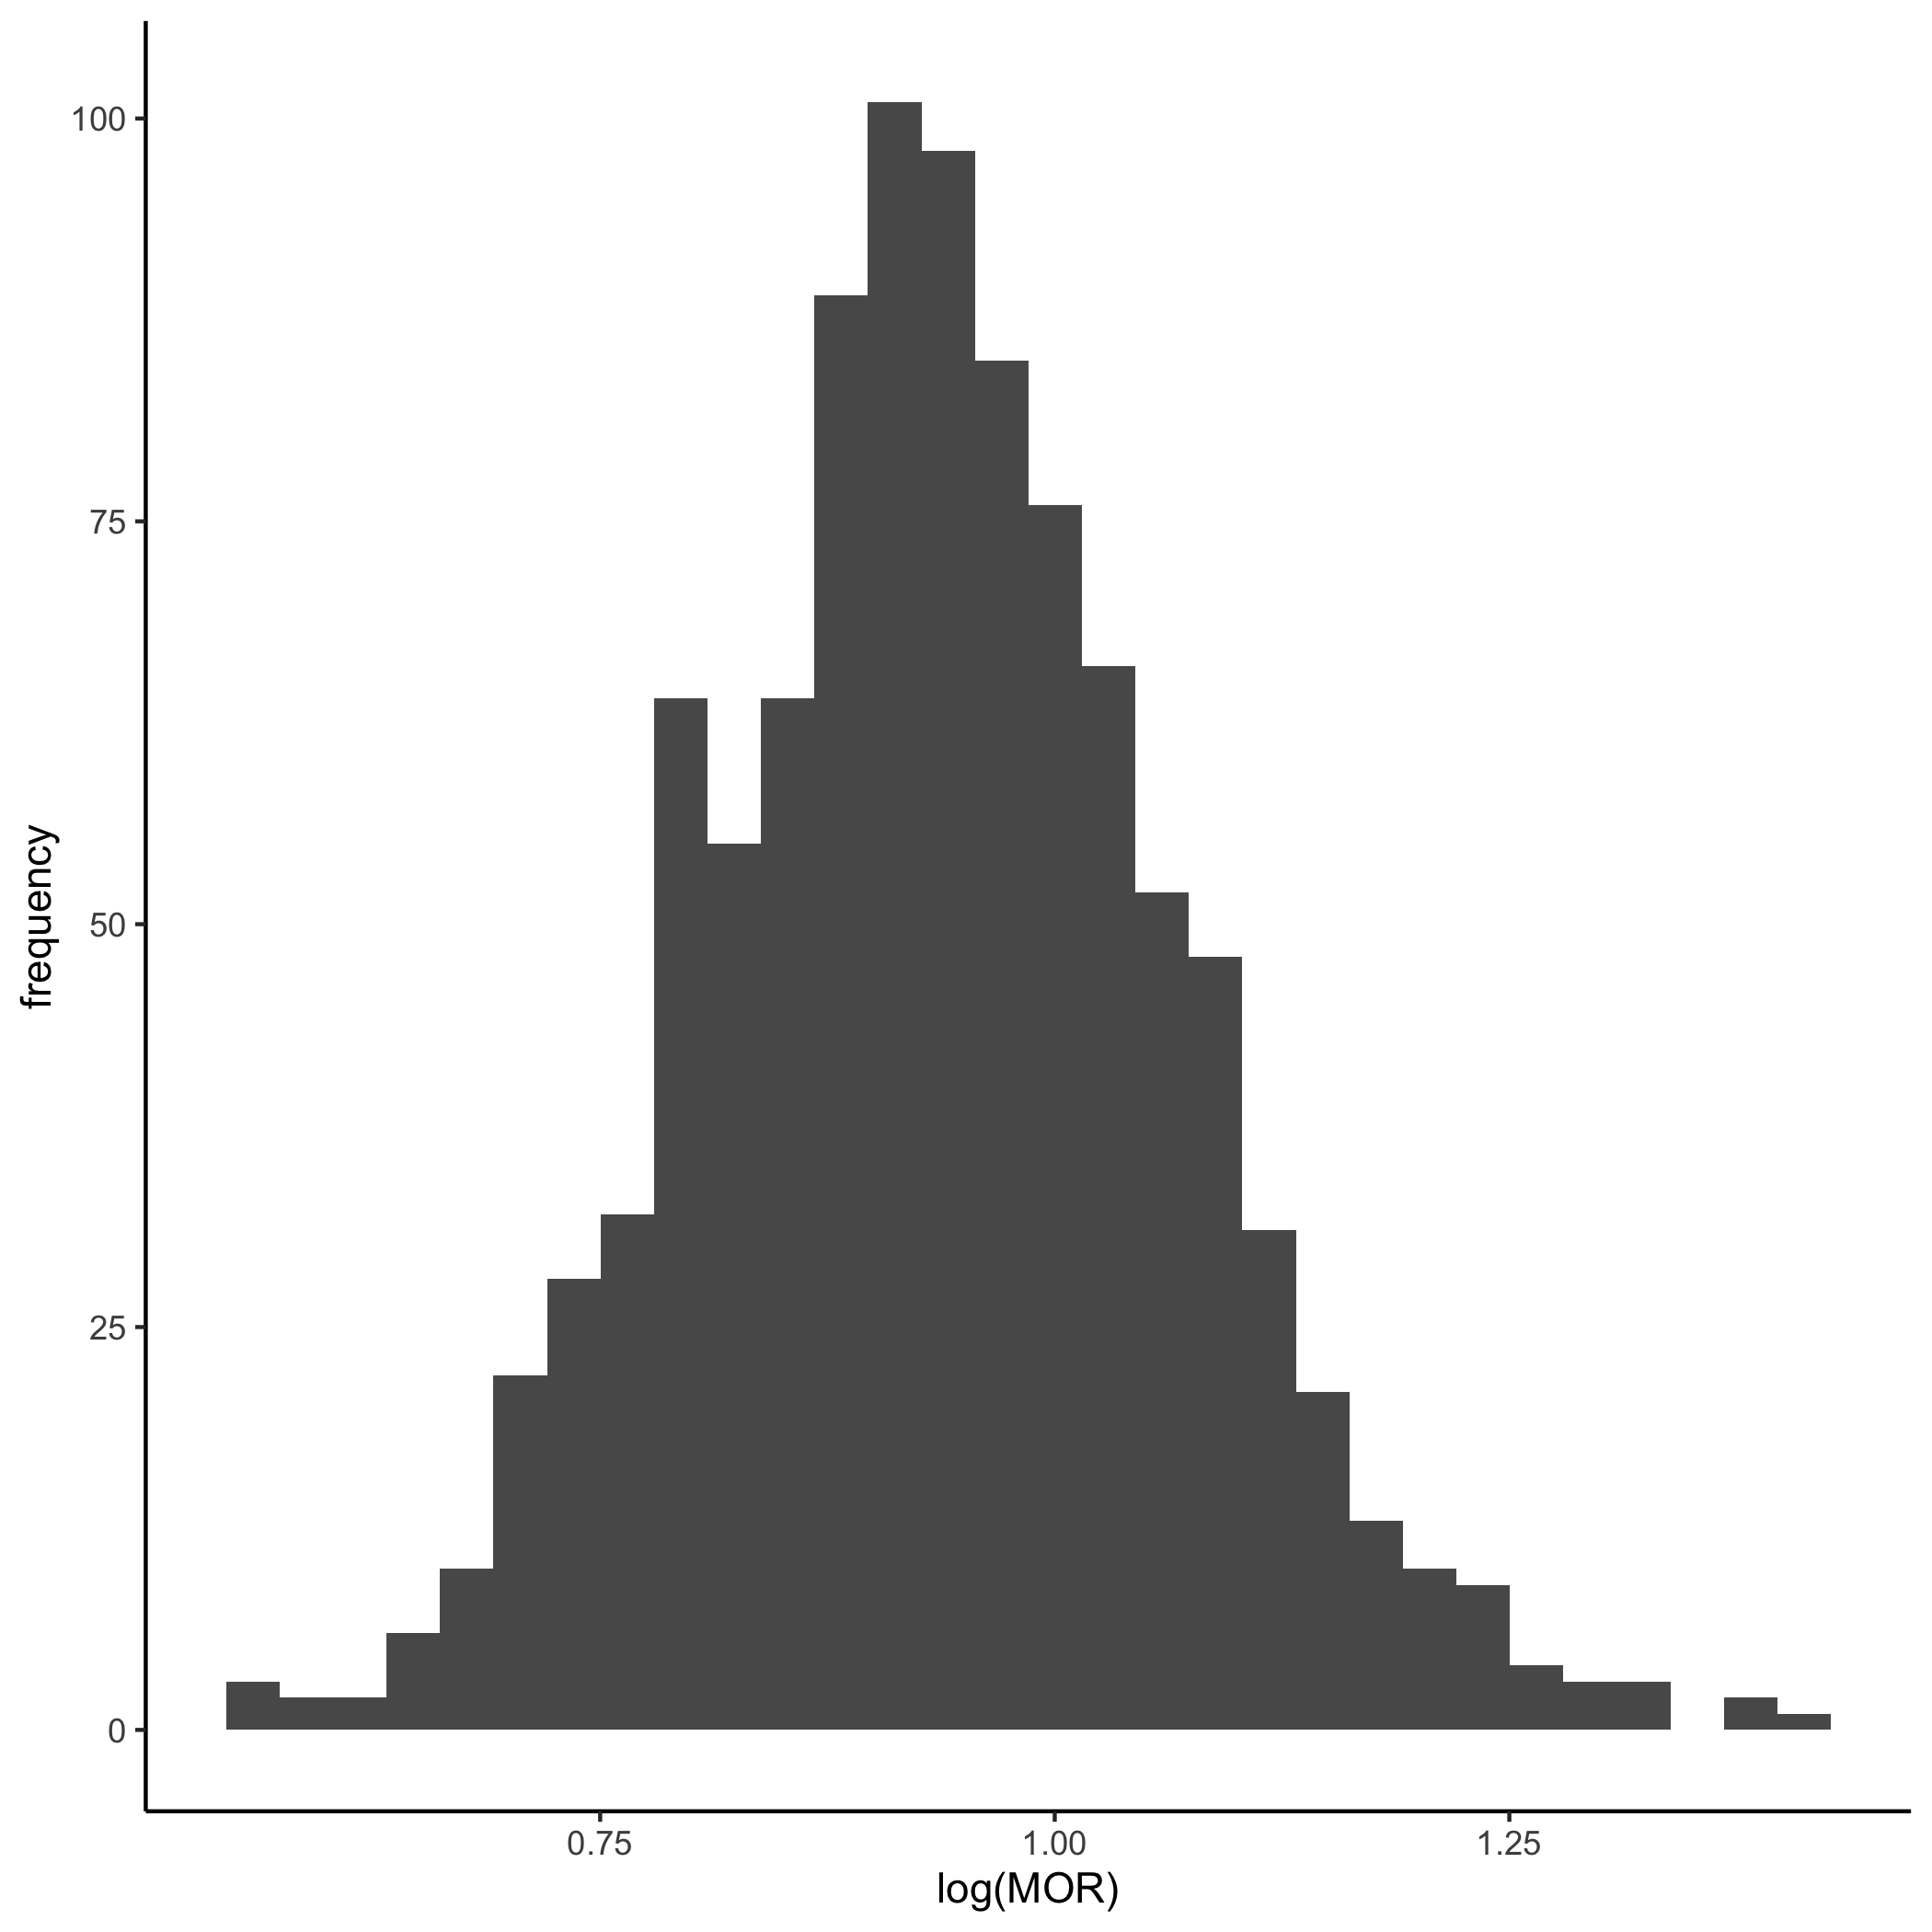
\includegraphics{../../plots/two-lvl-ran-slope/high-prev/hist_50_50_two_lvl_slp_high_prev_q2.png}

}

\caption{Cluster size 50}

}

\end{minipage}%
\newline
\begin{minipage}[t]{\linewidth}

{\centering 

~

}

\end{minipage}%
\newline
\begin{minipage}[t]{0.05\linewidth}

{\centering 

\rotatebox[origin=br]{90}{\tiny Cluster Number 100}

}

\end{minipage}%
%
\begin{minipage}[t]{0.24\linewidth}

{\centering 

\raisebox{-\height}{

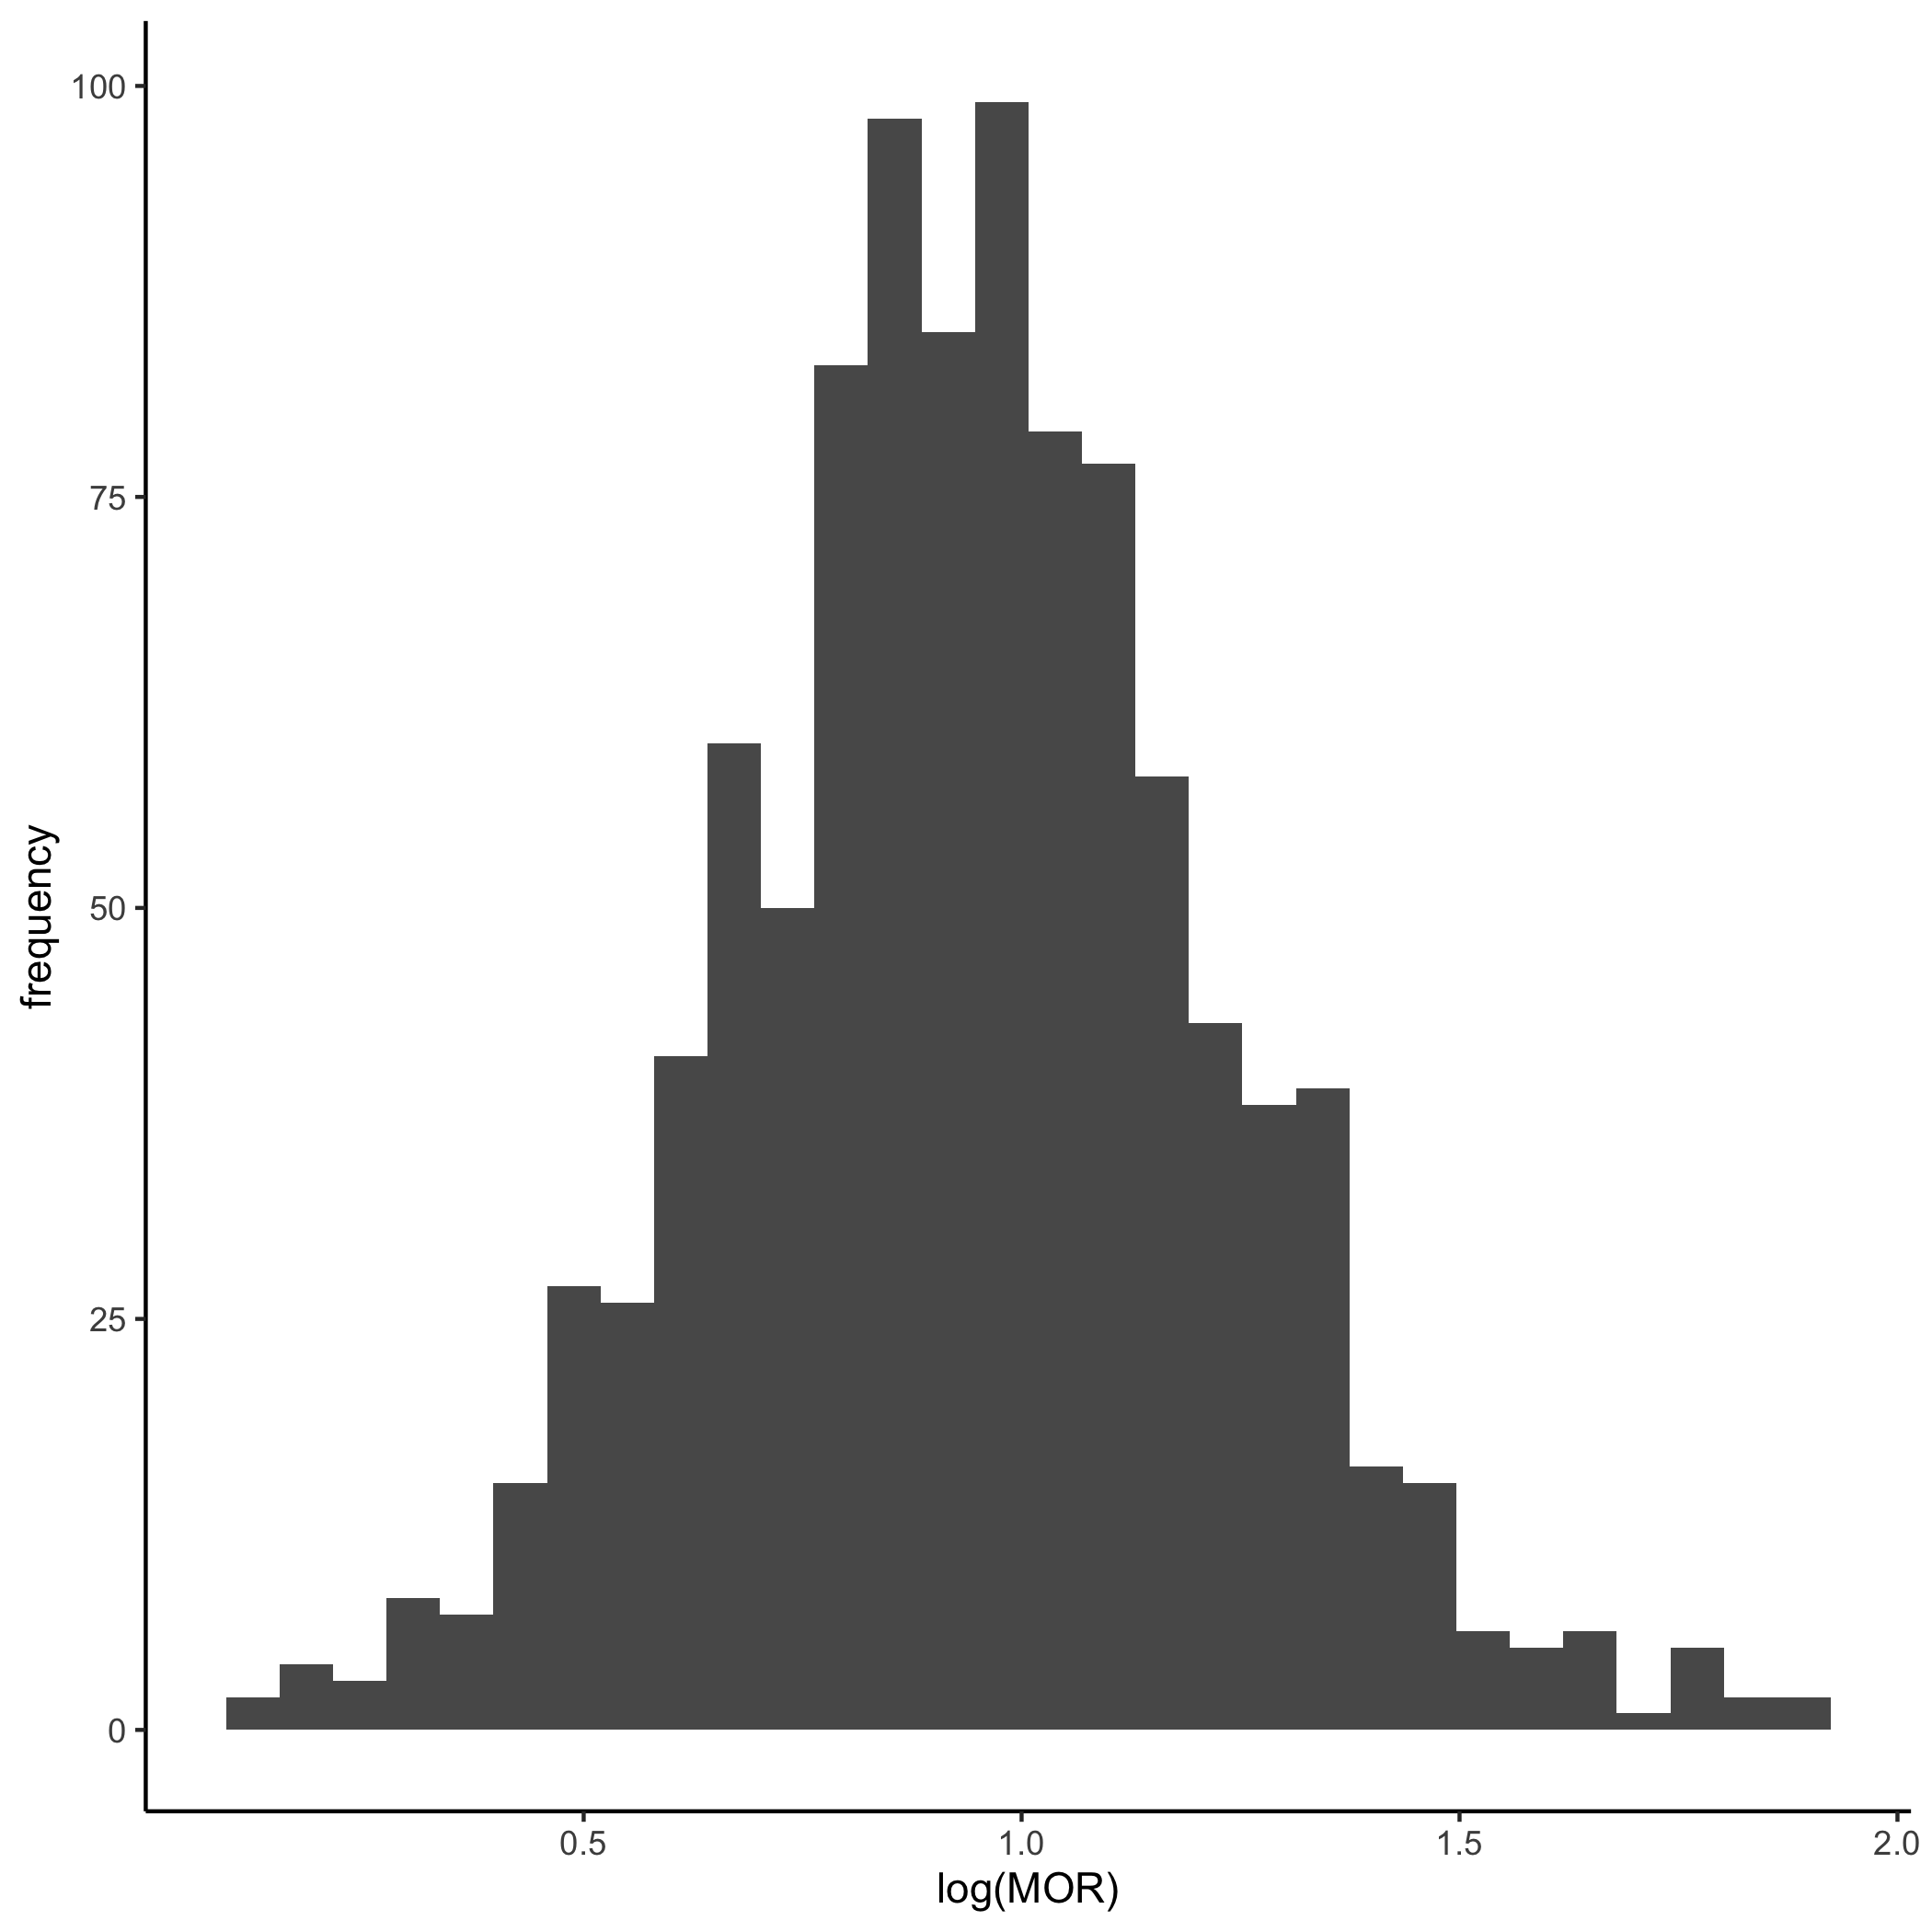
\includegraphics{../../plots/two-lvl-ran-slope/high-prev/hist_100_5_two_lvl_slp_high_prev_q2.png}

}

\caption{Cluster size 5}

}

\end{minipage}%
%
\begin{minipage}[t]{0.24\linewidth}

{\centering 

\raisebox{-\height}{

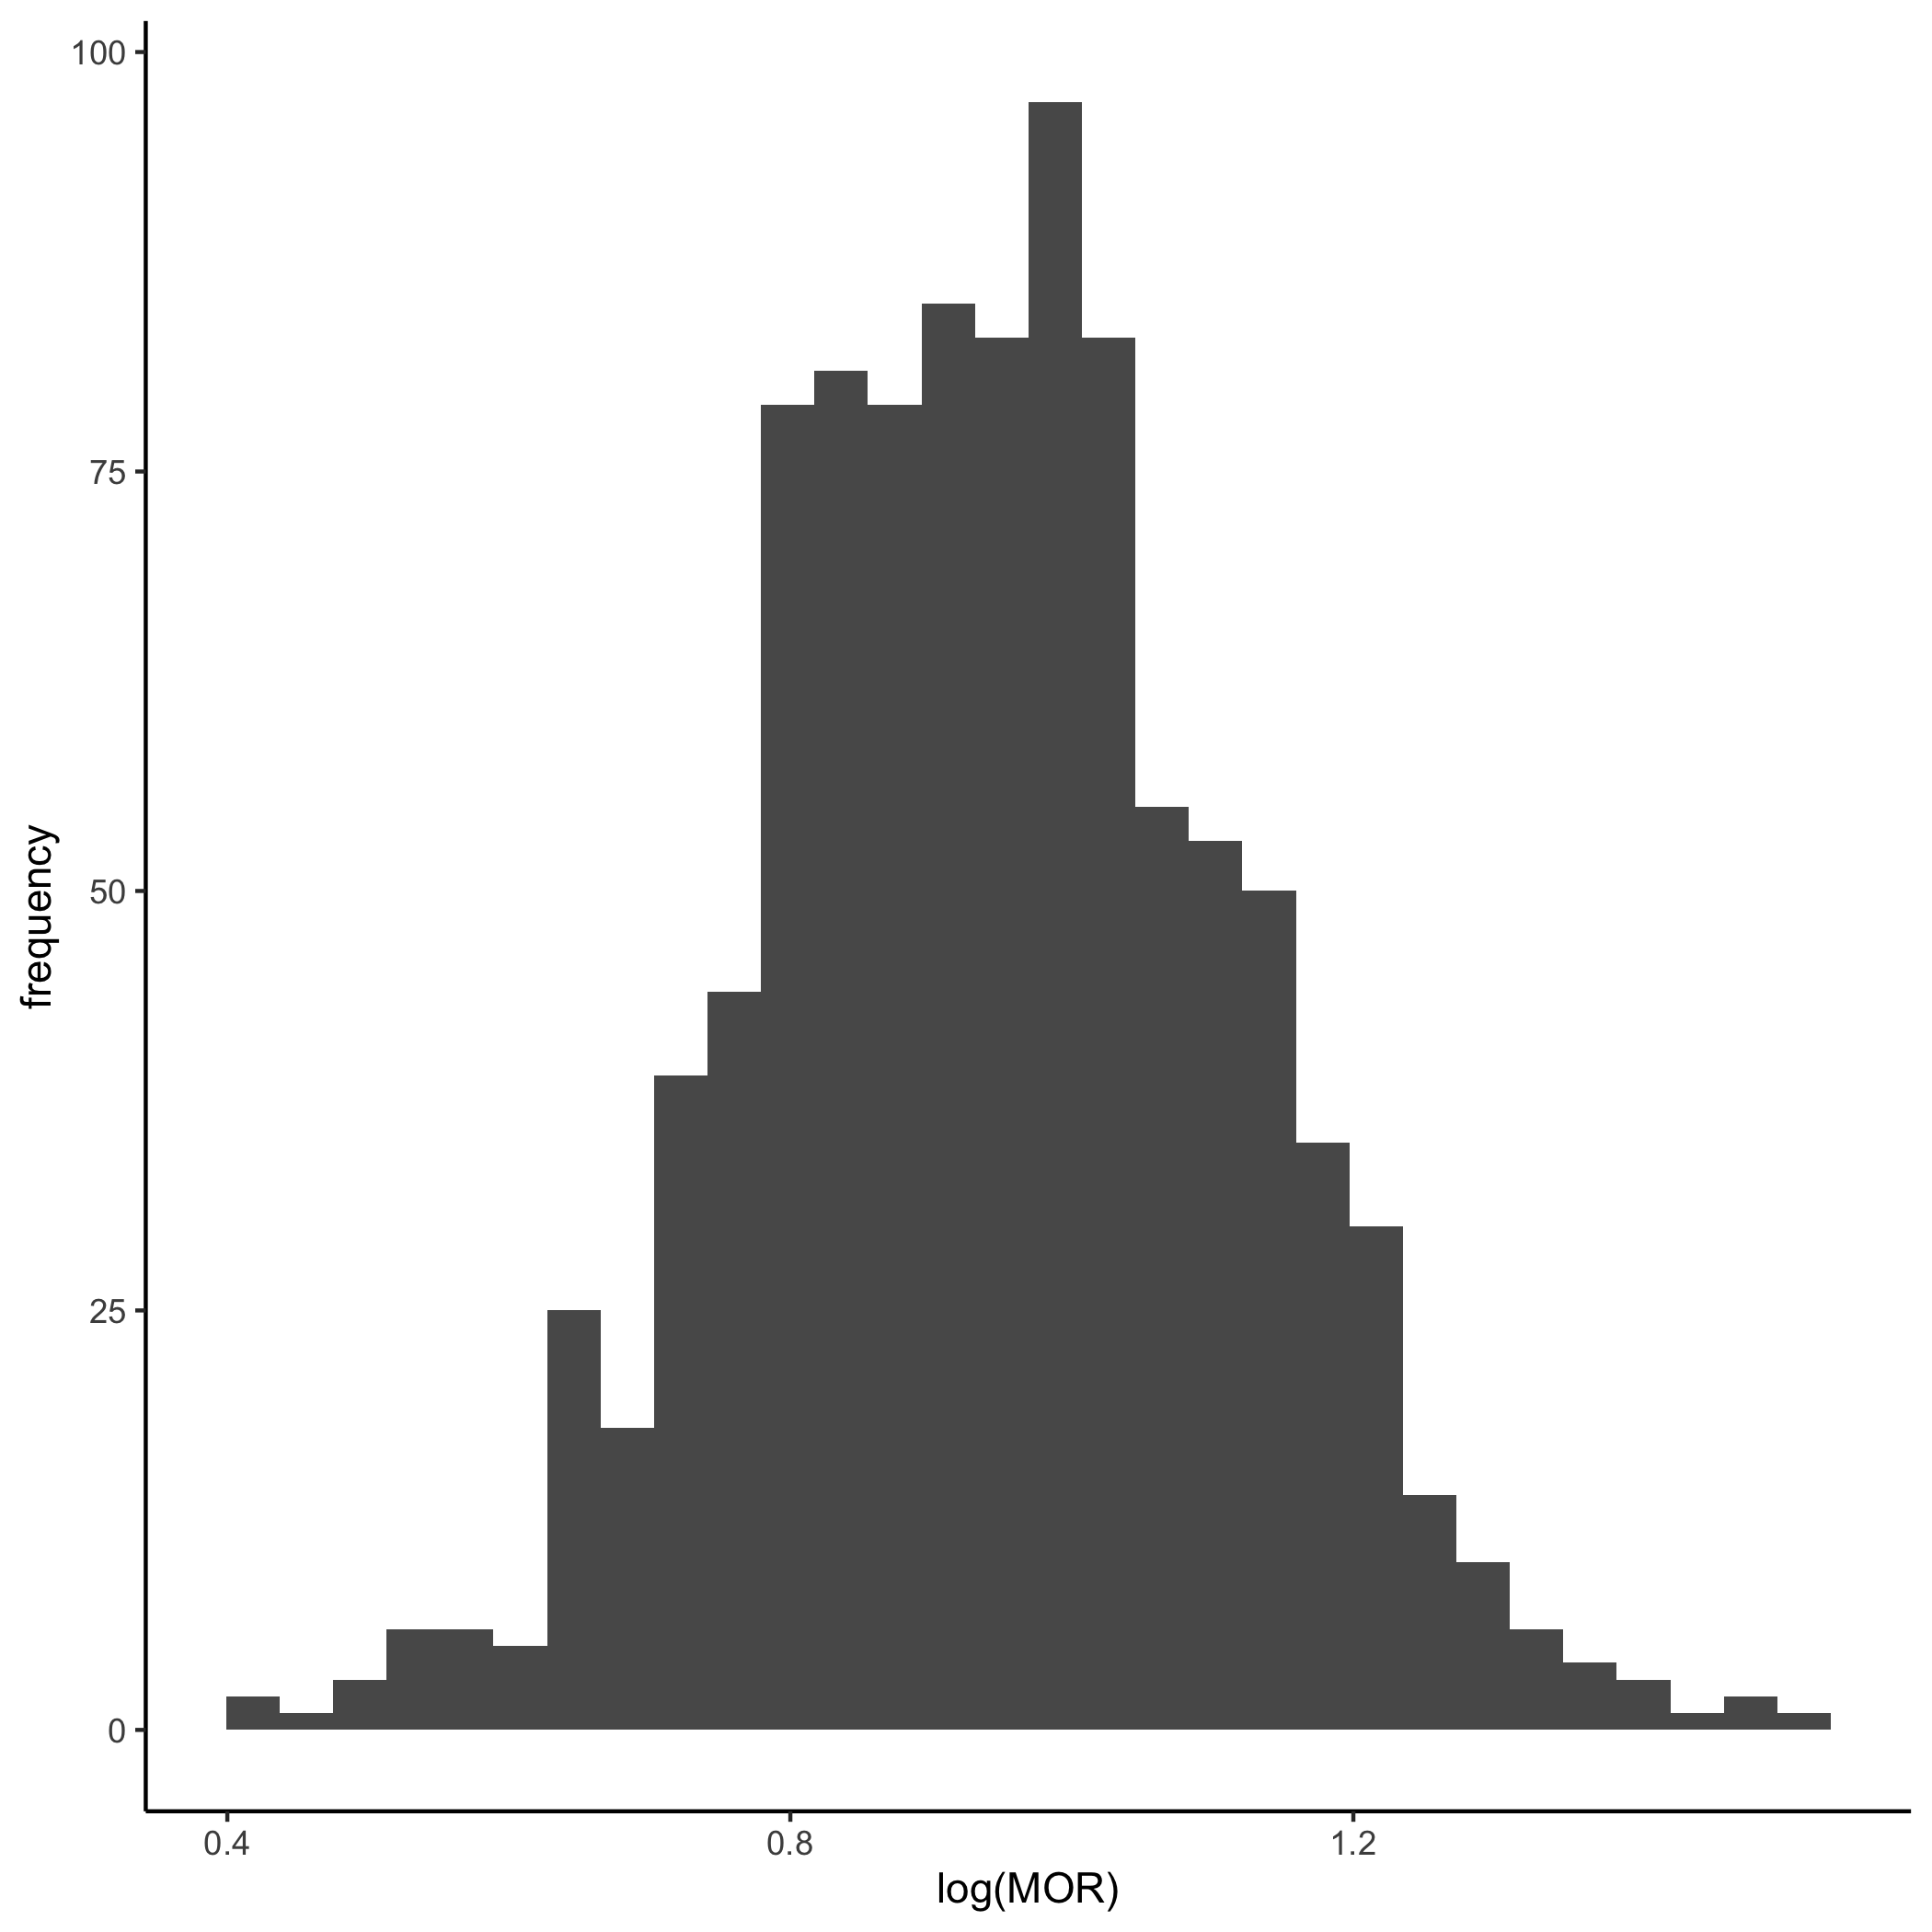
\includegraphics{../../plots/two-lvl-ran-slope/high-prev/hist_100_10_two_lvl_slp_high_prev_q2.png}

}

\caption{Cluster size 10}

}

\end{minipage}%
%
\begin{minipage}[t]{0.24\linewidth}

{\centering 

\raisebox{-\height}{

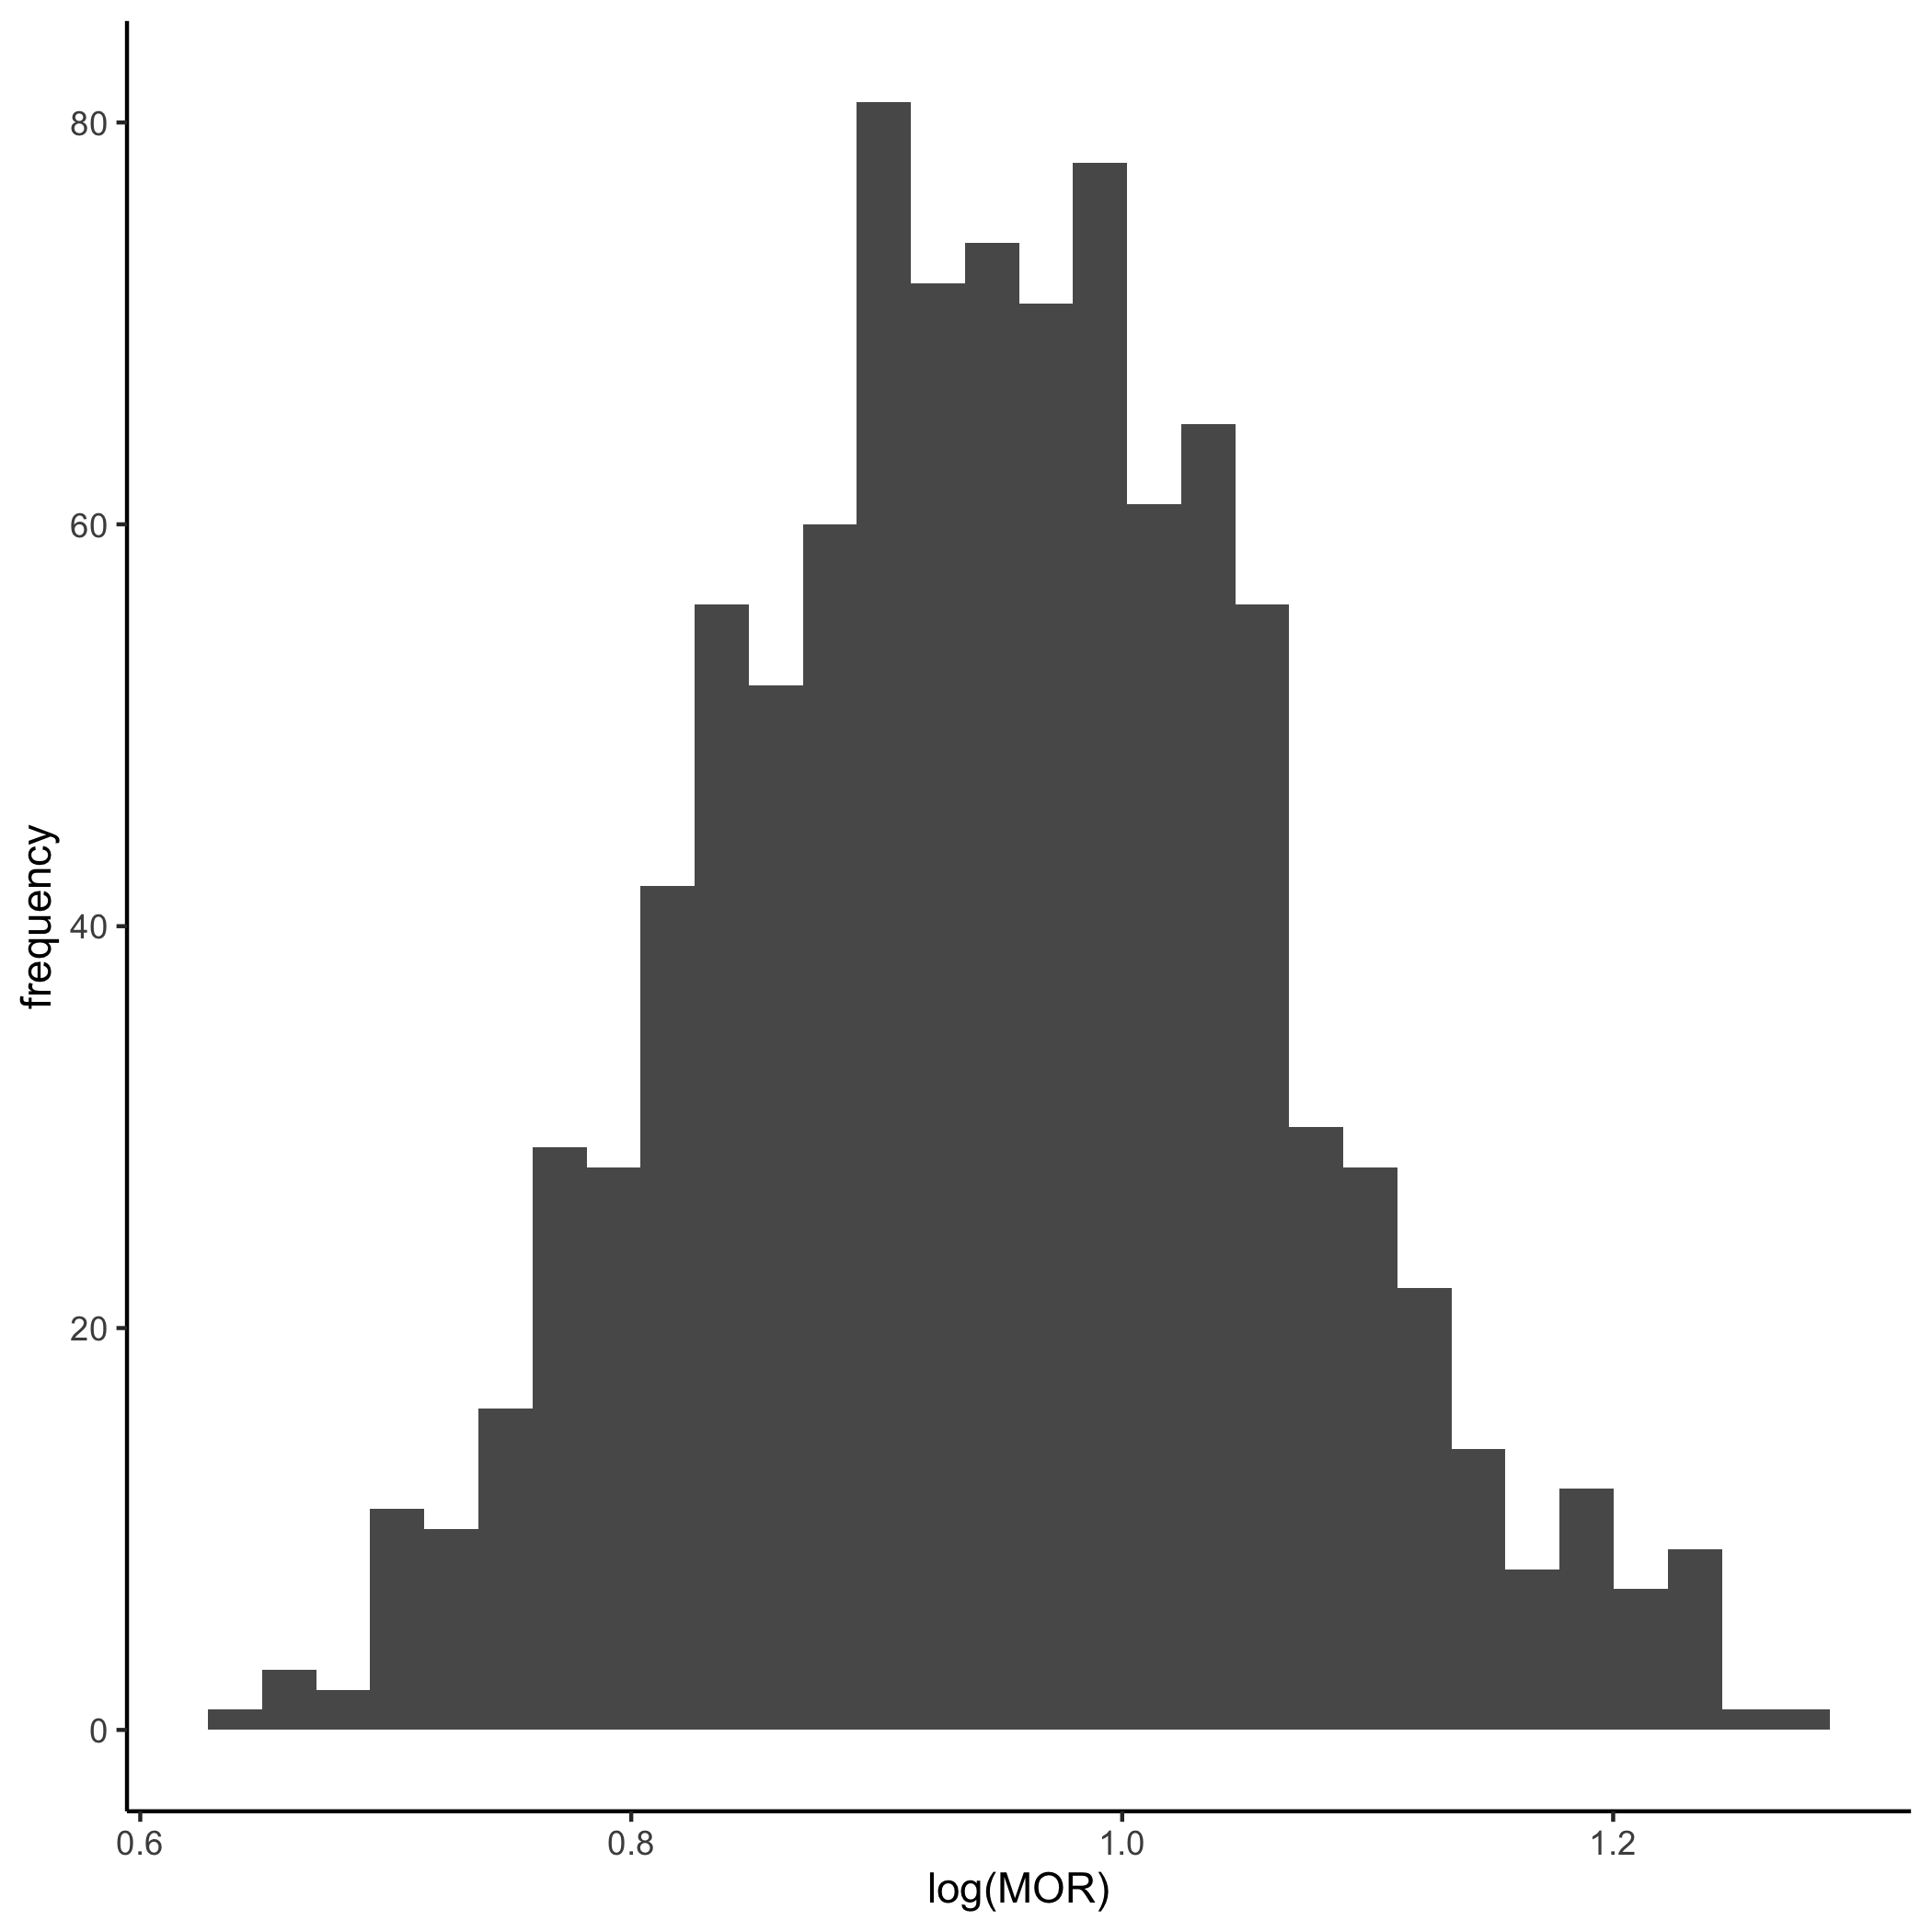
\includegraphics{../../plots/two-lvl-ran-slope/high-prev/hist_100_30_two_lvl_slp_high_prev_q2.png}

}

\caption{Cluster size 30}

}

\end{minipage}%
%
\begin{minipage}[t]{0.24\linewidth}

{\centering 

\raisebox{-\height}{

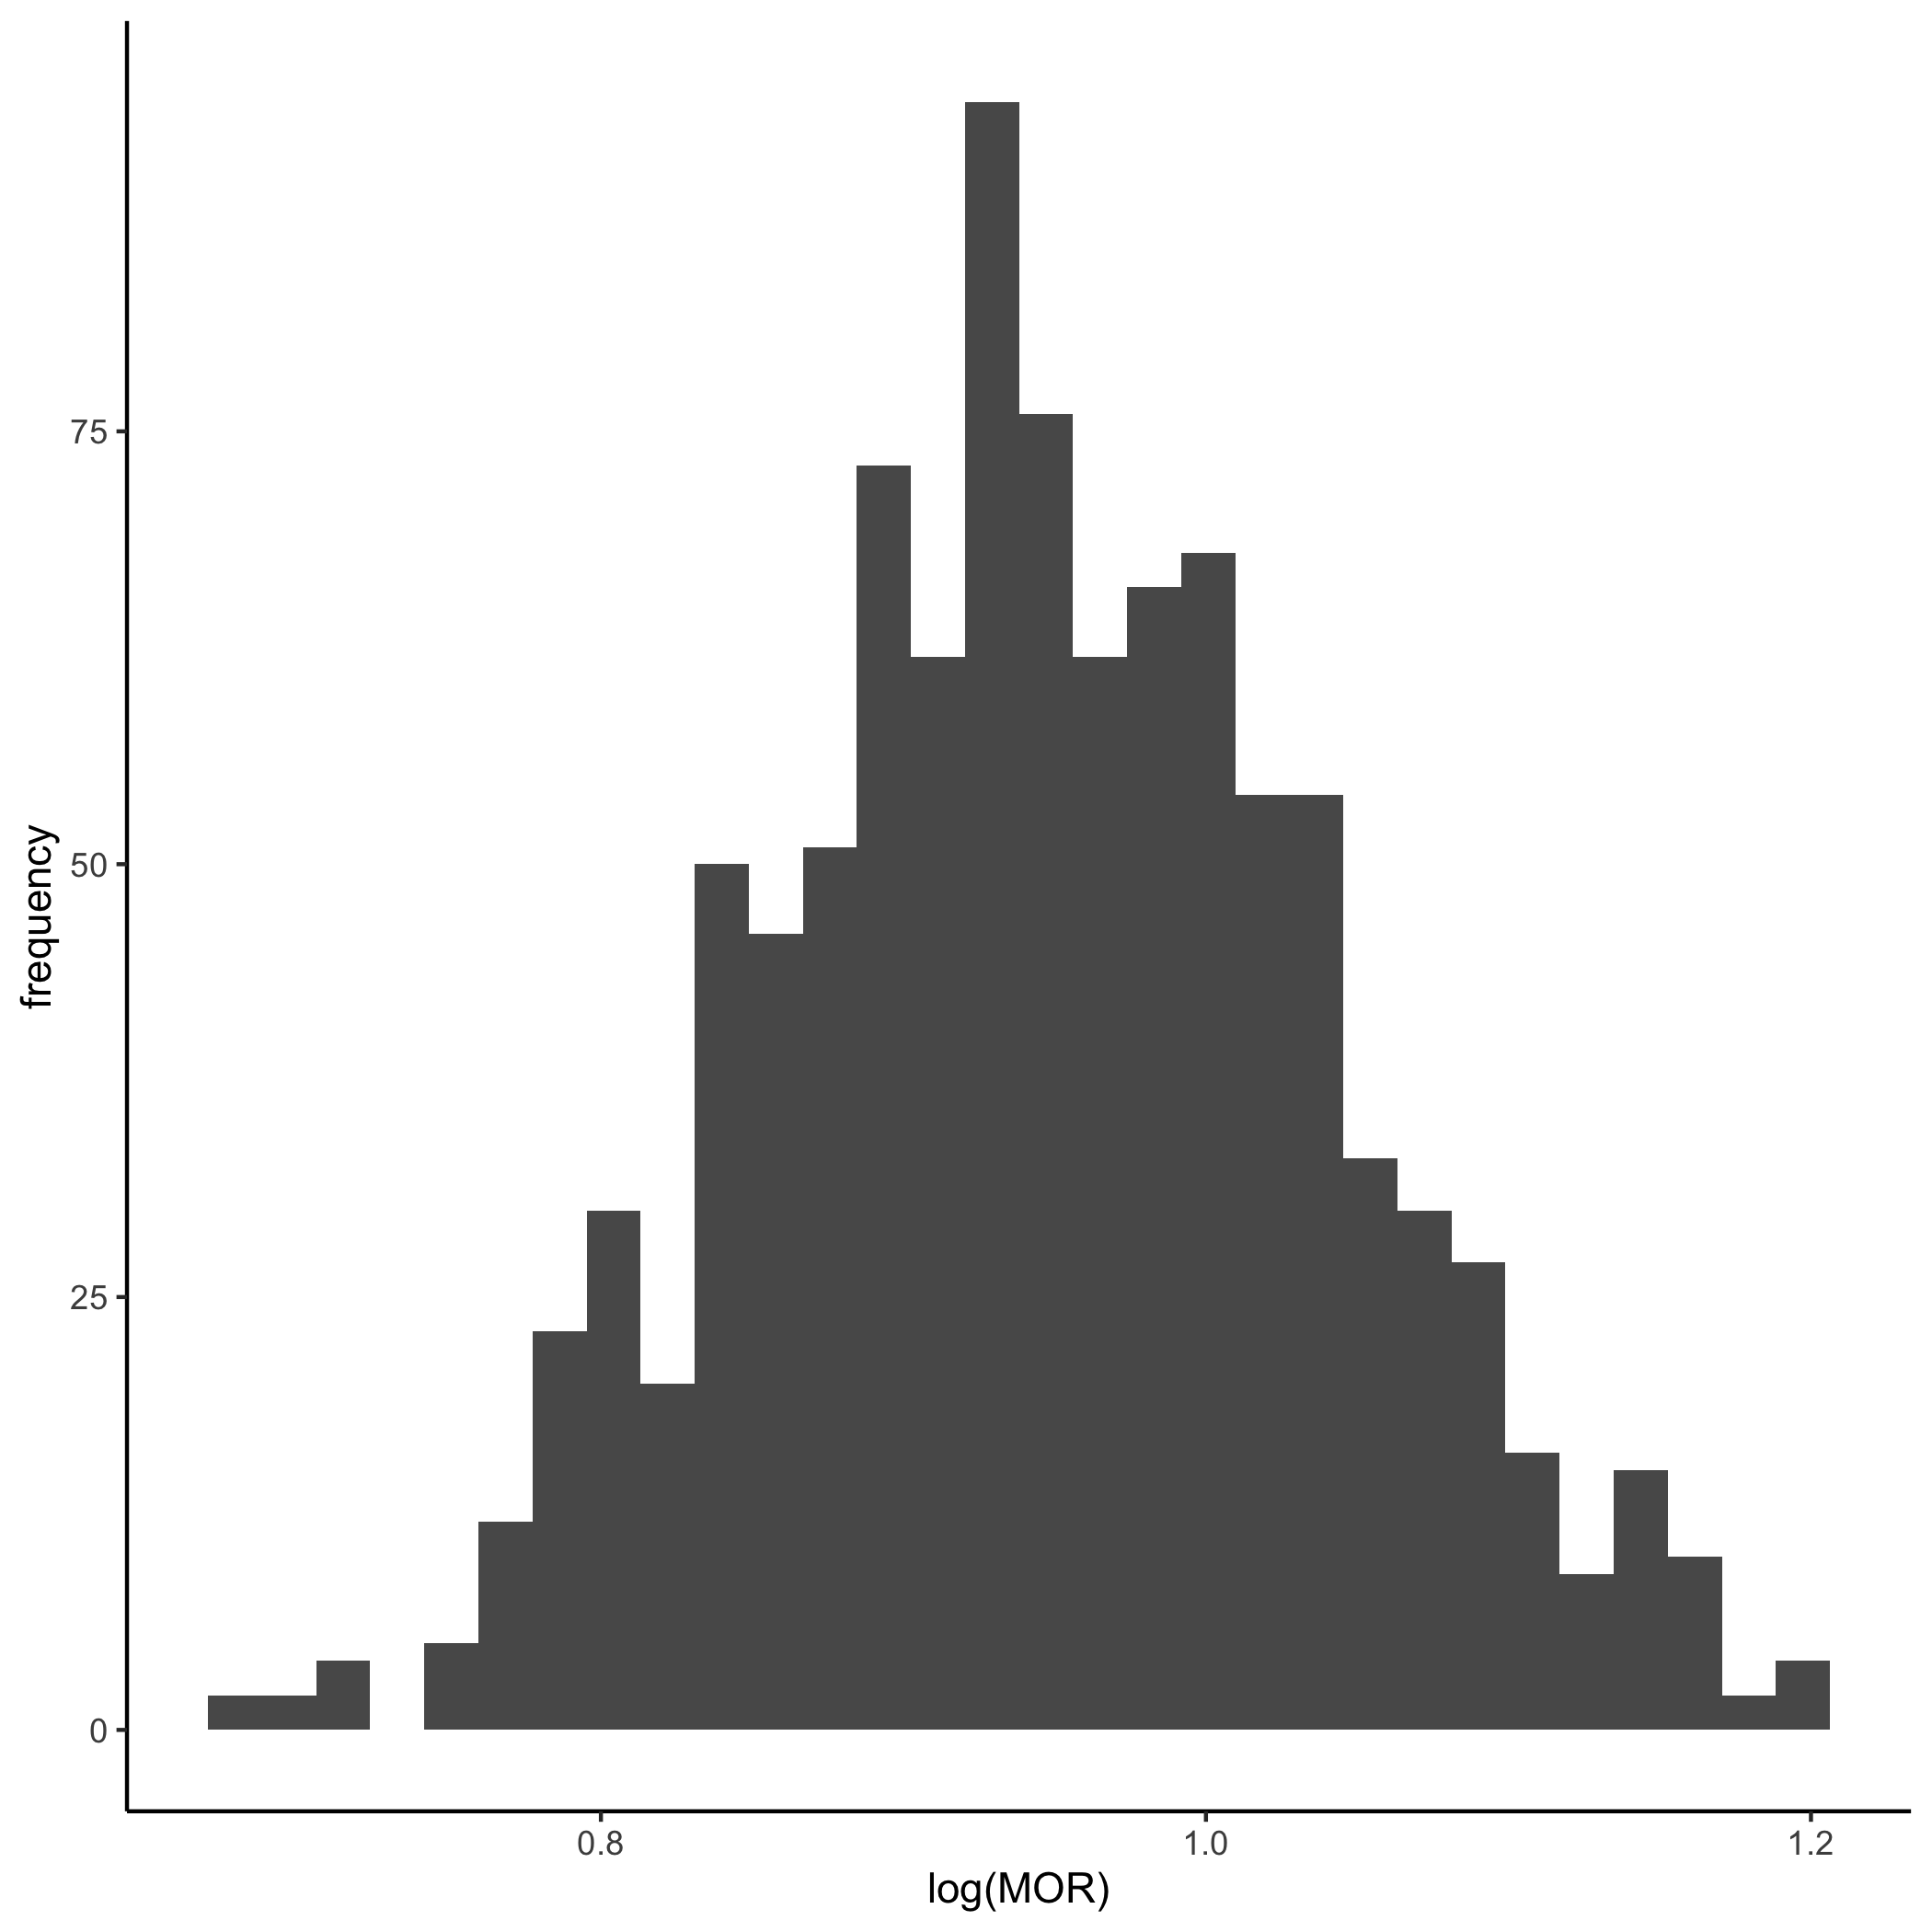
\includegraphics{../../plots/two-lvl-ran-slope/high-prev/hist_100_50_two_lvl_slp_high_prev_q2.png}

}

\caption{Cluster size 50}

}

\end{minipage}%

\end{figure}

\newpage

\hypertarget{histograms-for-logwidehatmor-when-third-quartile-of-x-is-used}{%
\section{\texorpdfstring{Histograms for \(log(\widehat{MOR})\) when
Third Quartile of \(X\) is
used}{Histograms for log(\textbackslash widehat\{MOR\}) when Third Quartile of X is used}}\label{histograms-for-logwidehatmor-when-third-quartile-of-x-is-used}}

\vspace{10mm}

\begin{figure}

\begin{minipage}[t]{0.05\linewidth}

{\centering 

\rotatebox[origin=br]{90}{\tiny Cluster Number 10}

}

\end{minipage}%
%
\begin{minipage}[t]{0.24\linewidth}

{\centering 

\raisebox{-\height}{

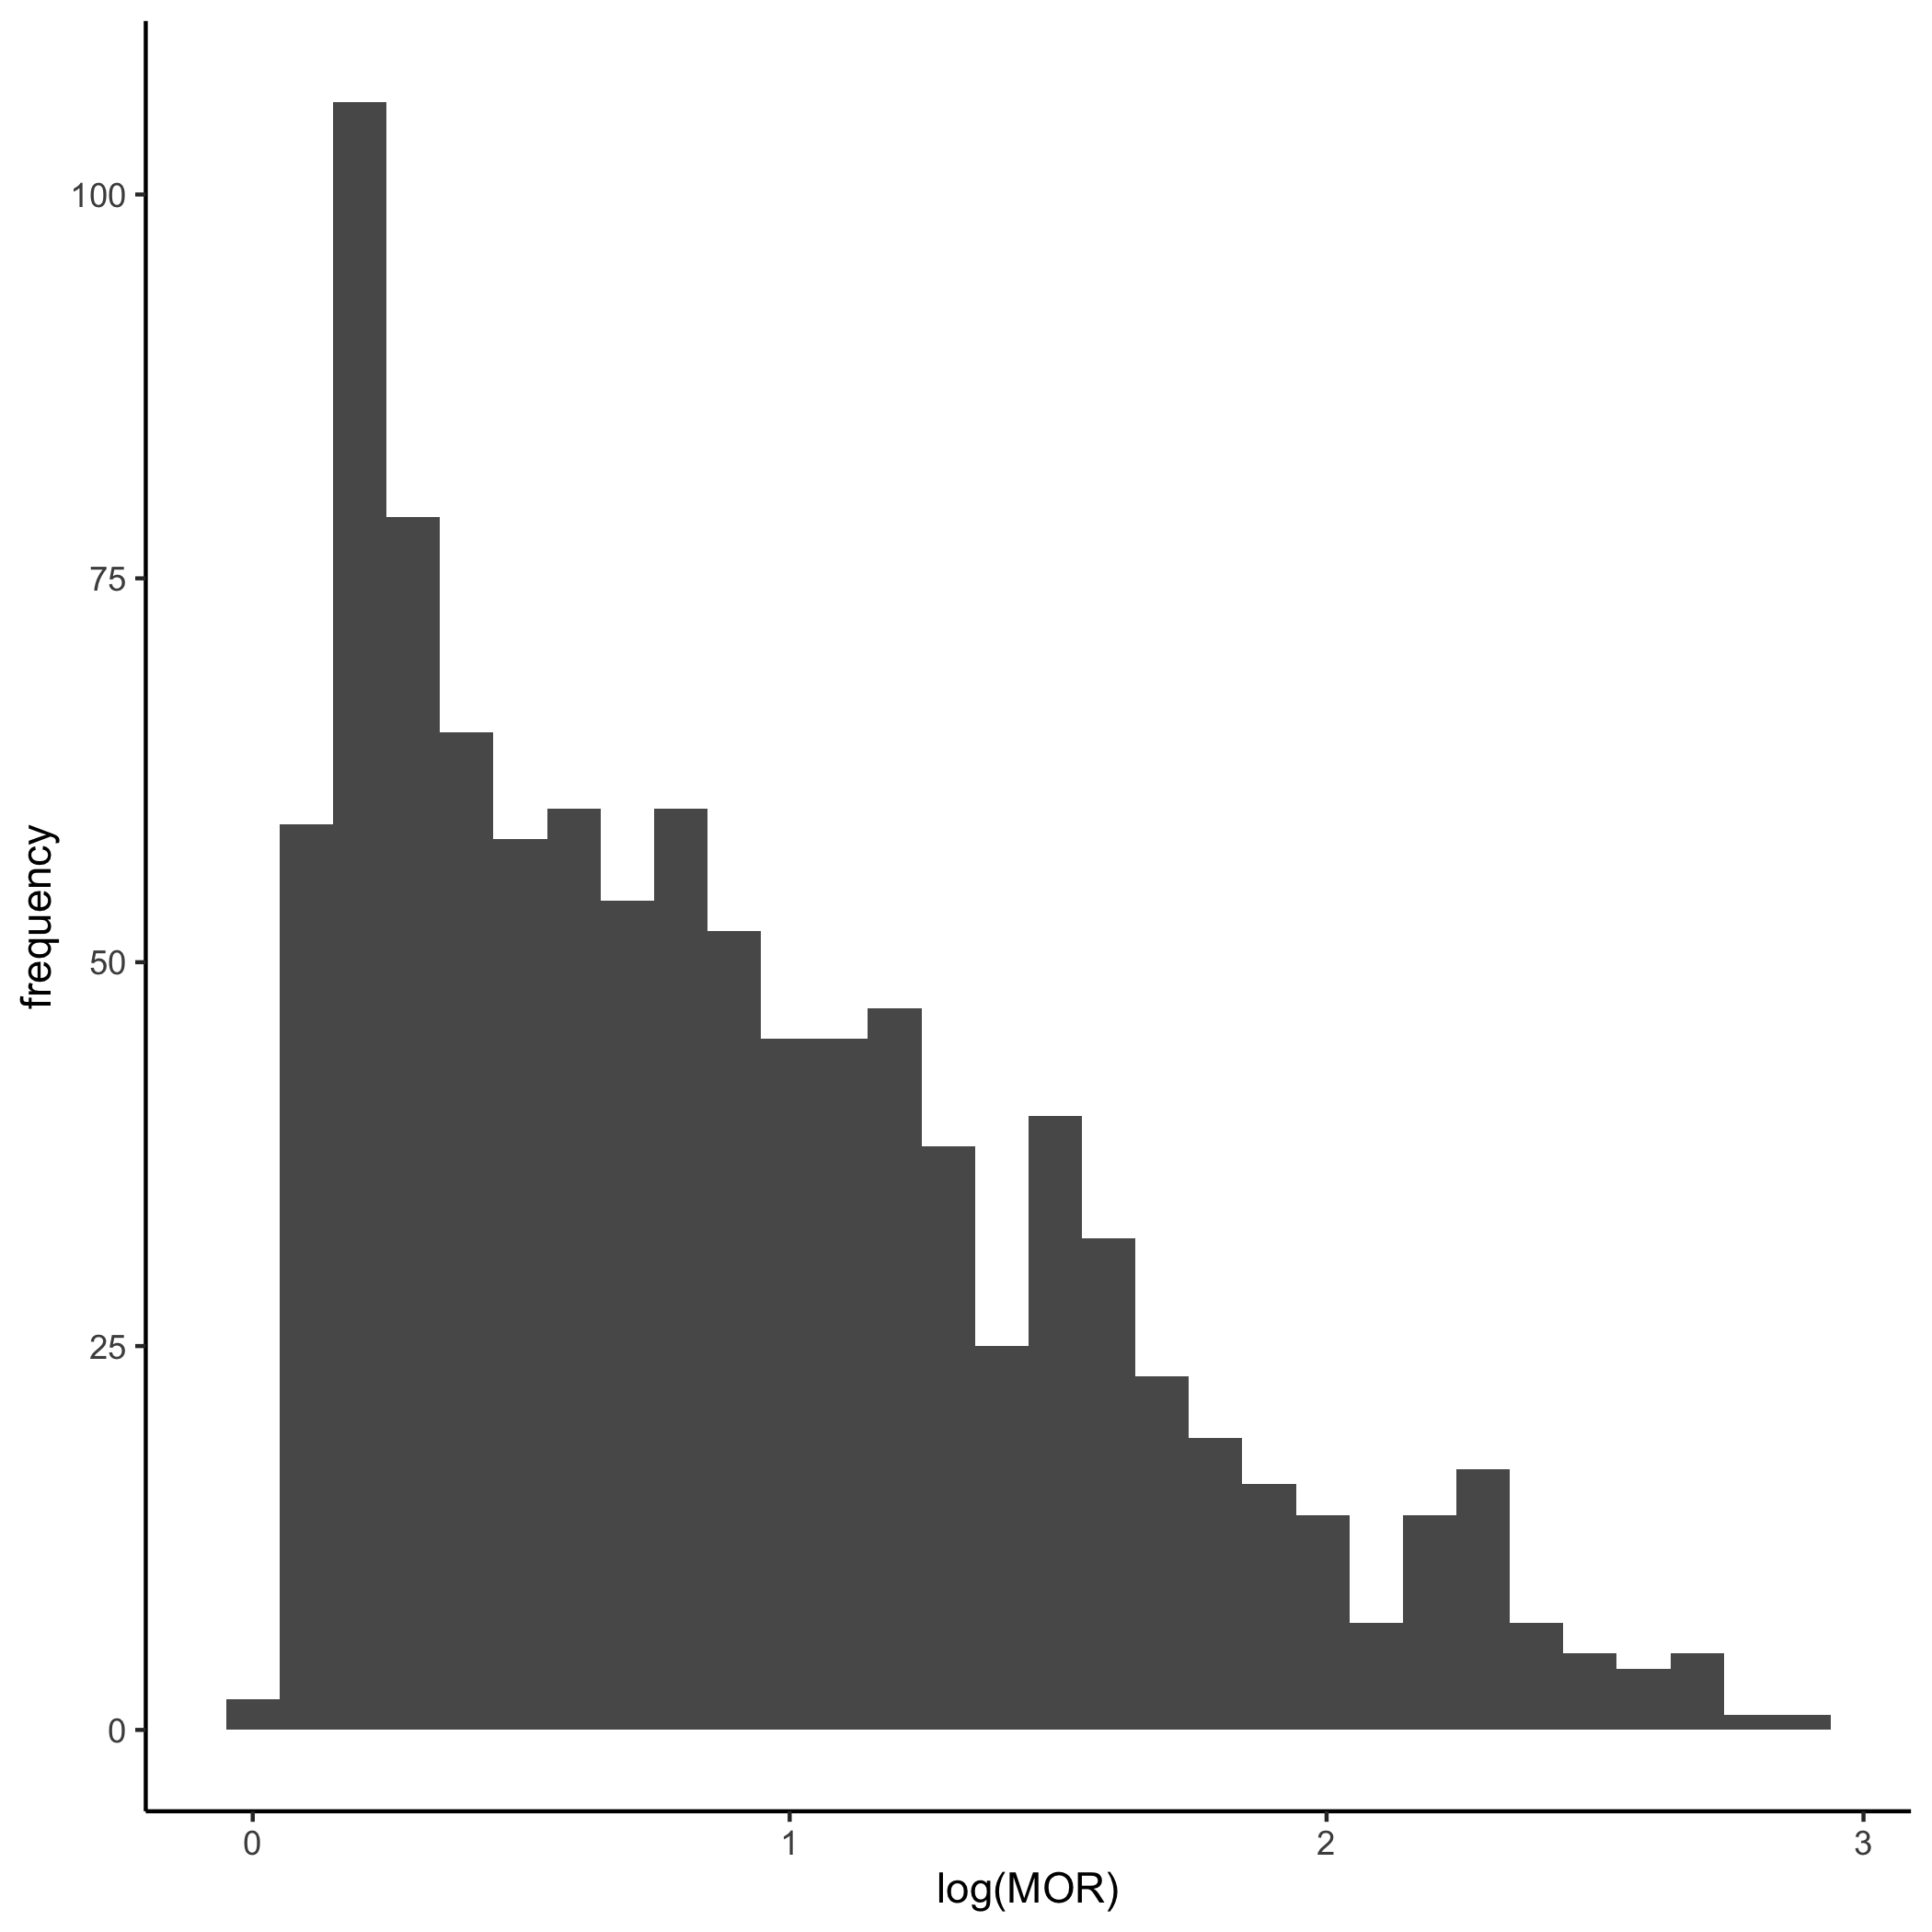
\includegraphics{../../plots/two-lvl-ran-slope/high-prev/hist_10_5_two_lvl_slp_high_prev_q3.png}

}

\caption{Cluster size 5}

}

\end{minipage}%
%
\begin{minipage}[t]{0.24\linewidth}

{\centering 

\raisebox{-\height}{

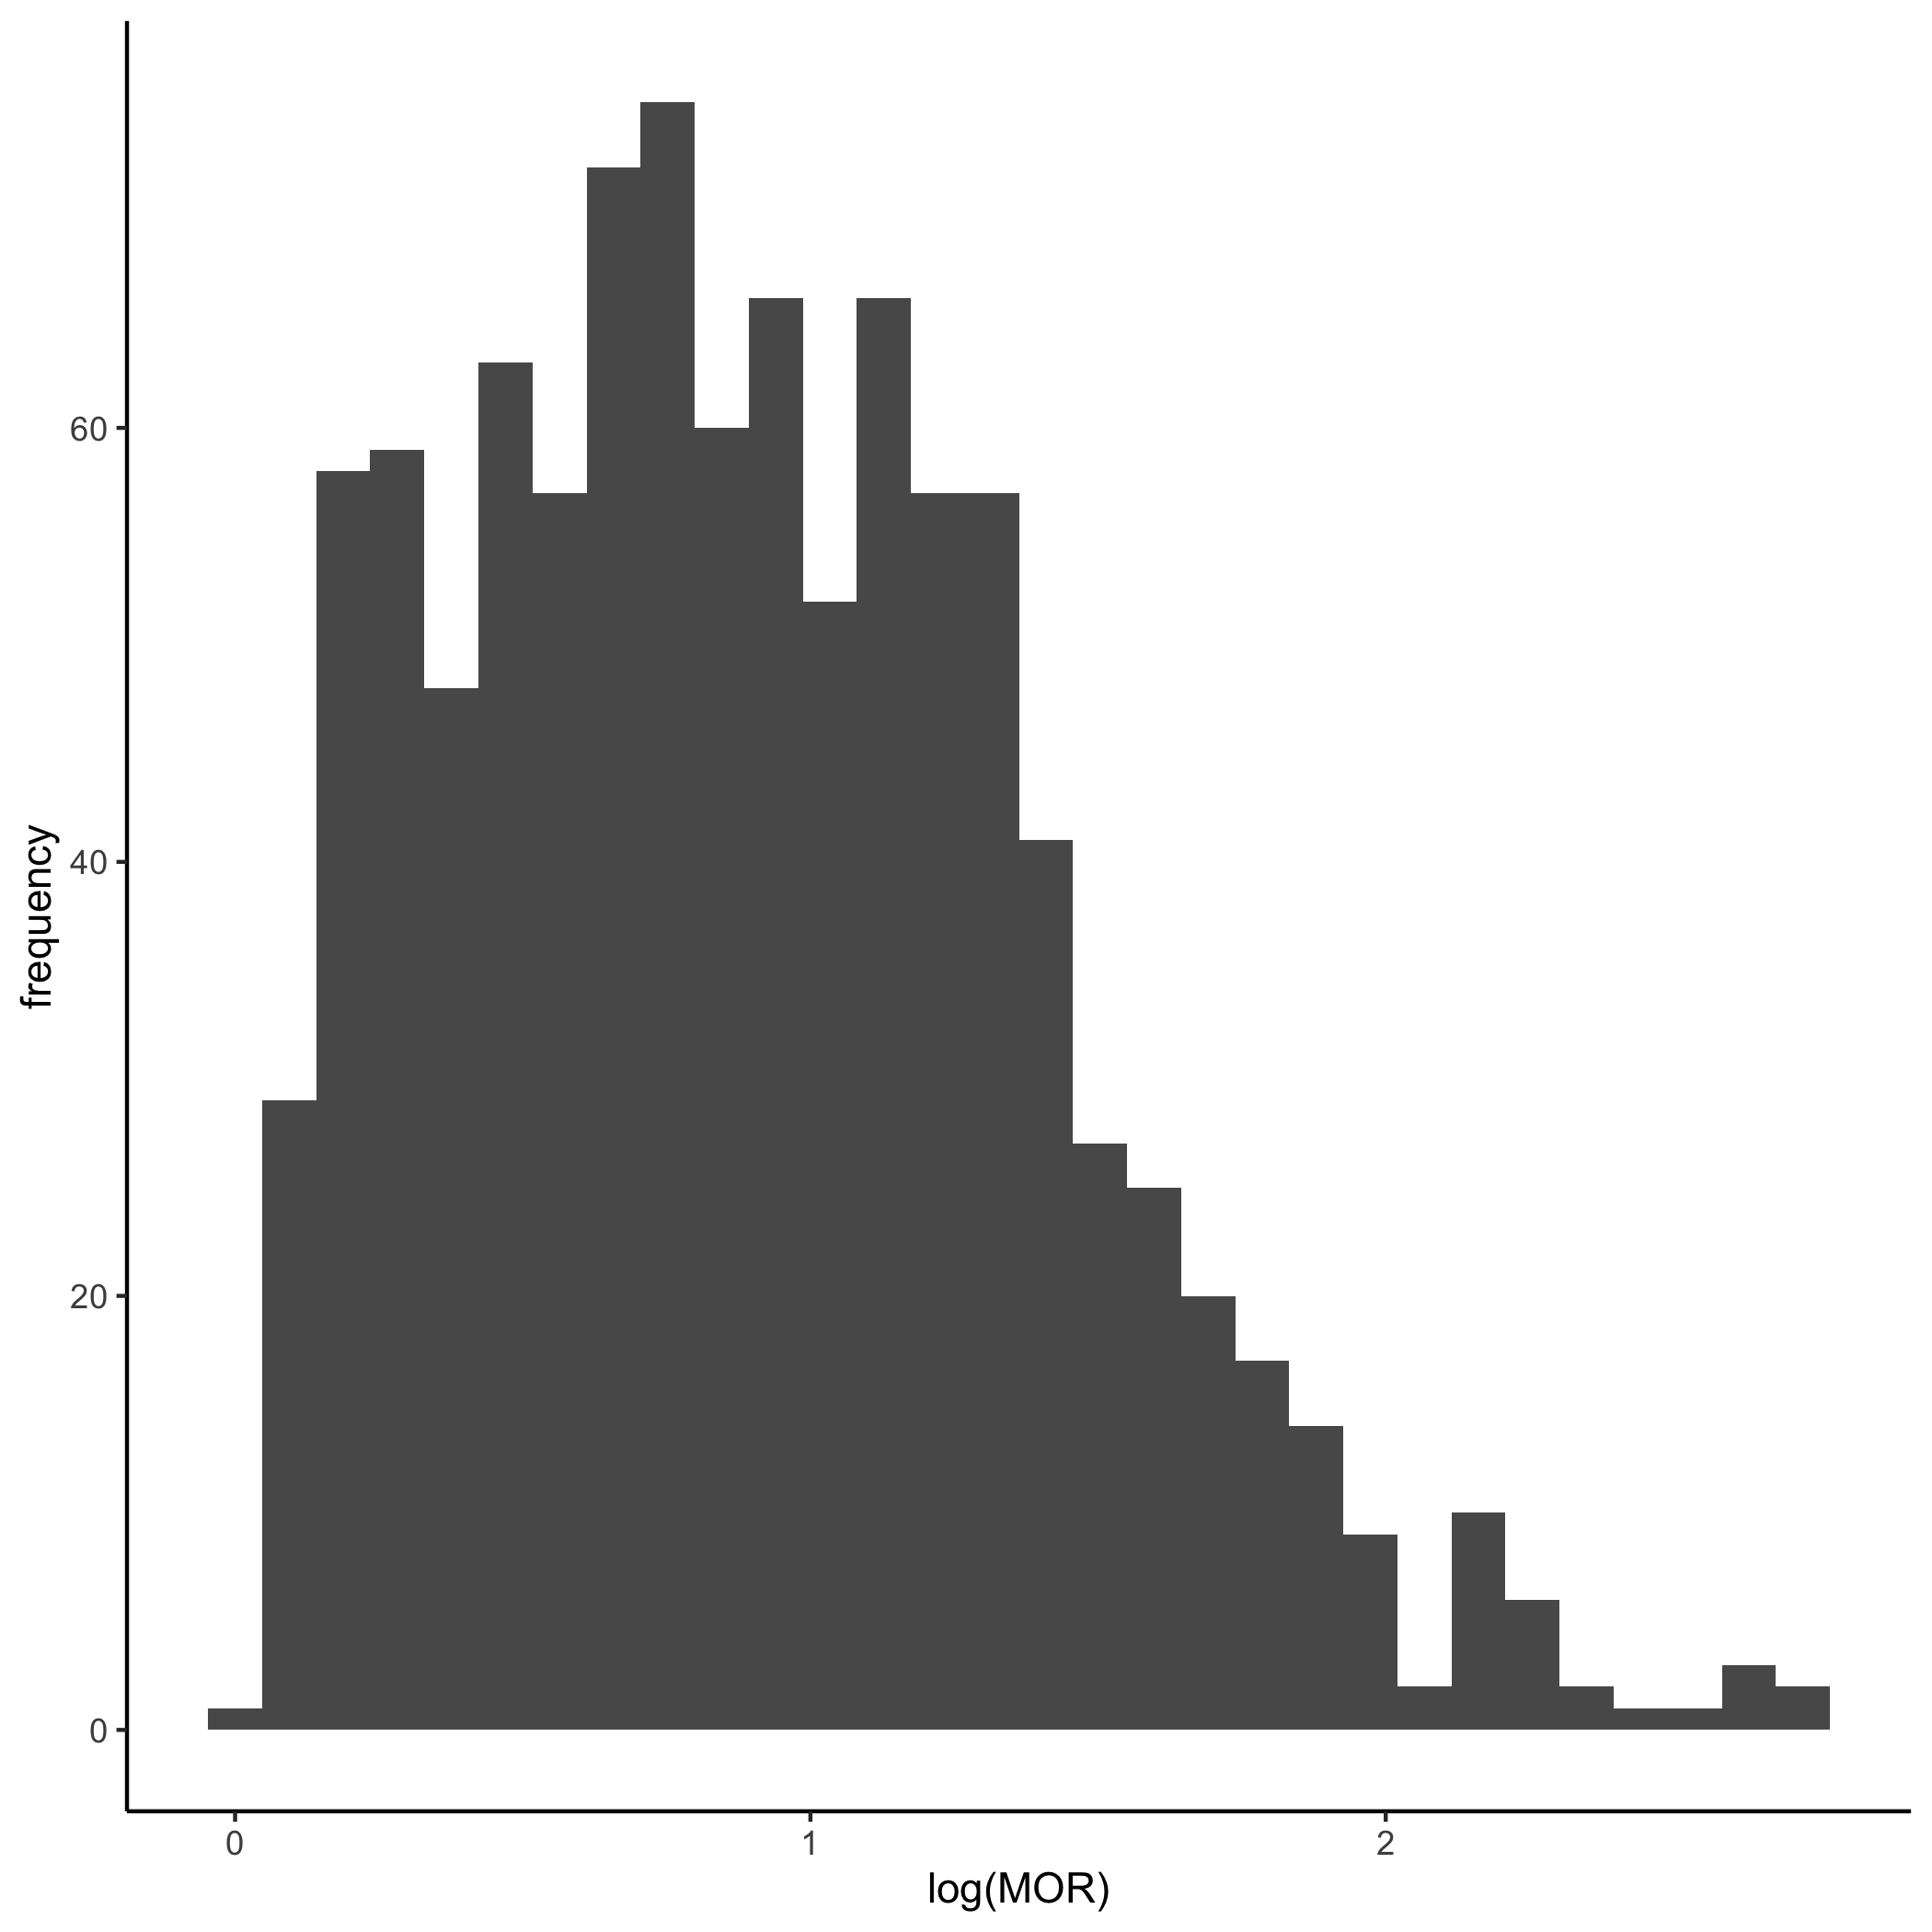
\includegraphics{../../plots/two-lvl-ran-slope/high-prev/hist_10_10_two_lvl_slp_high_prev_q3.png}

}

\caption{Cluster size 10}

}

\end{minipage}%
%
\begin{minipage}[t]{0.24\linewidth}

{\centering 

\raisebox{-\height}{

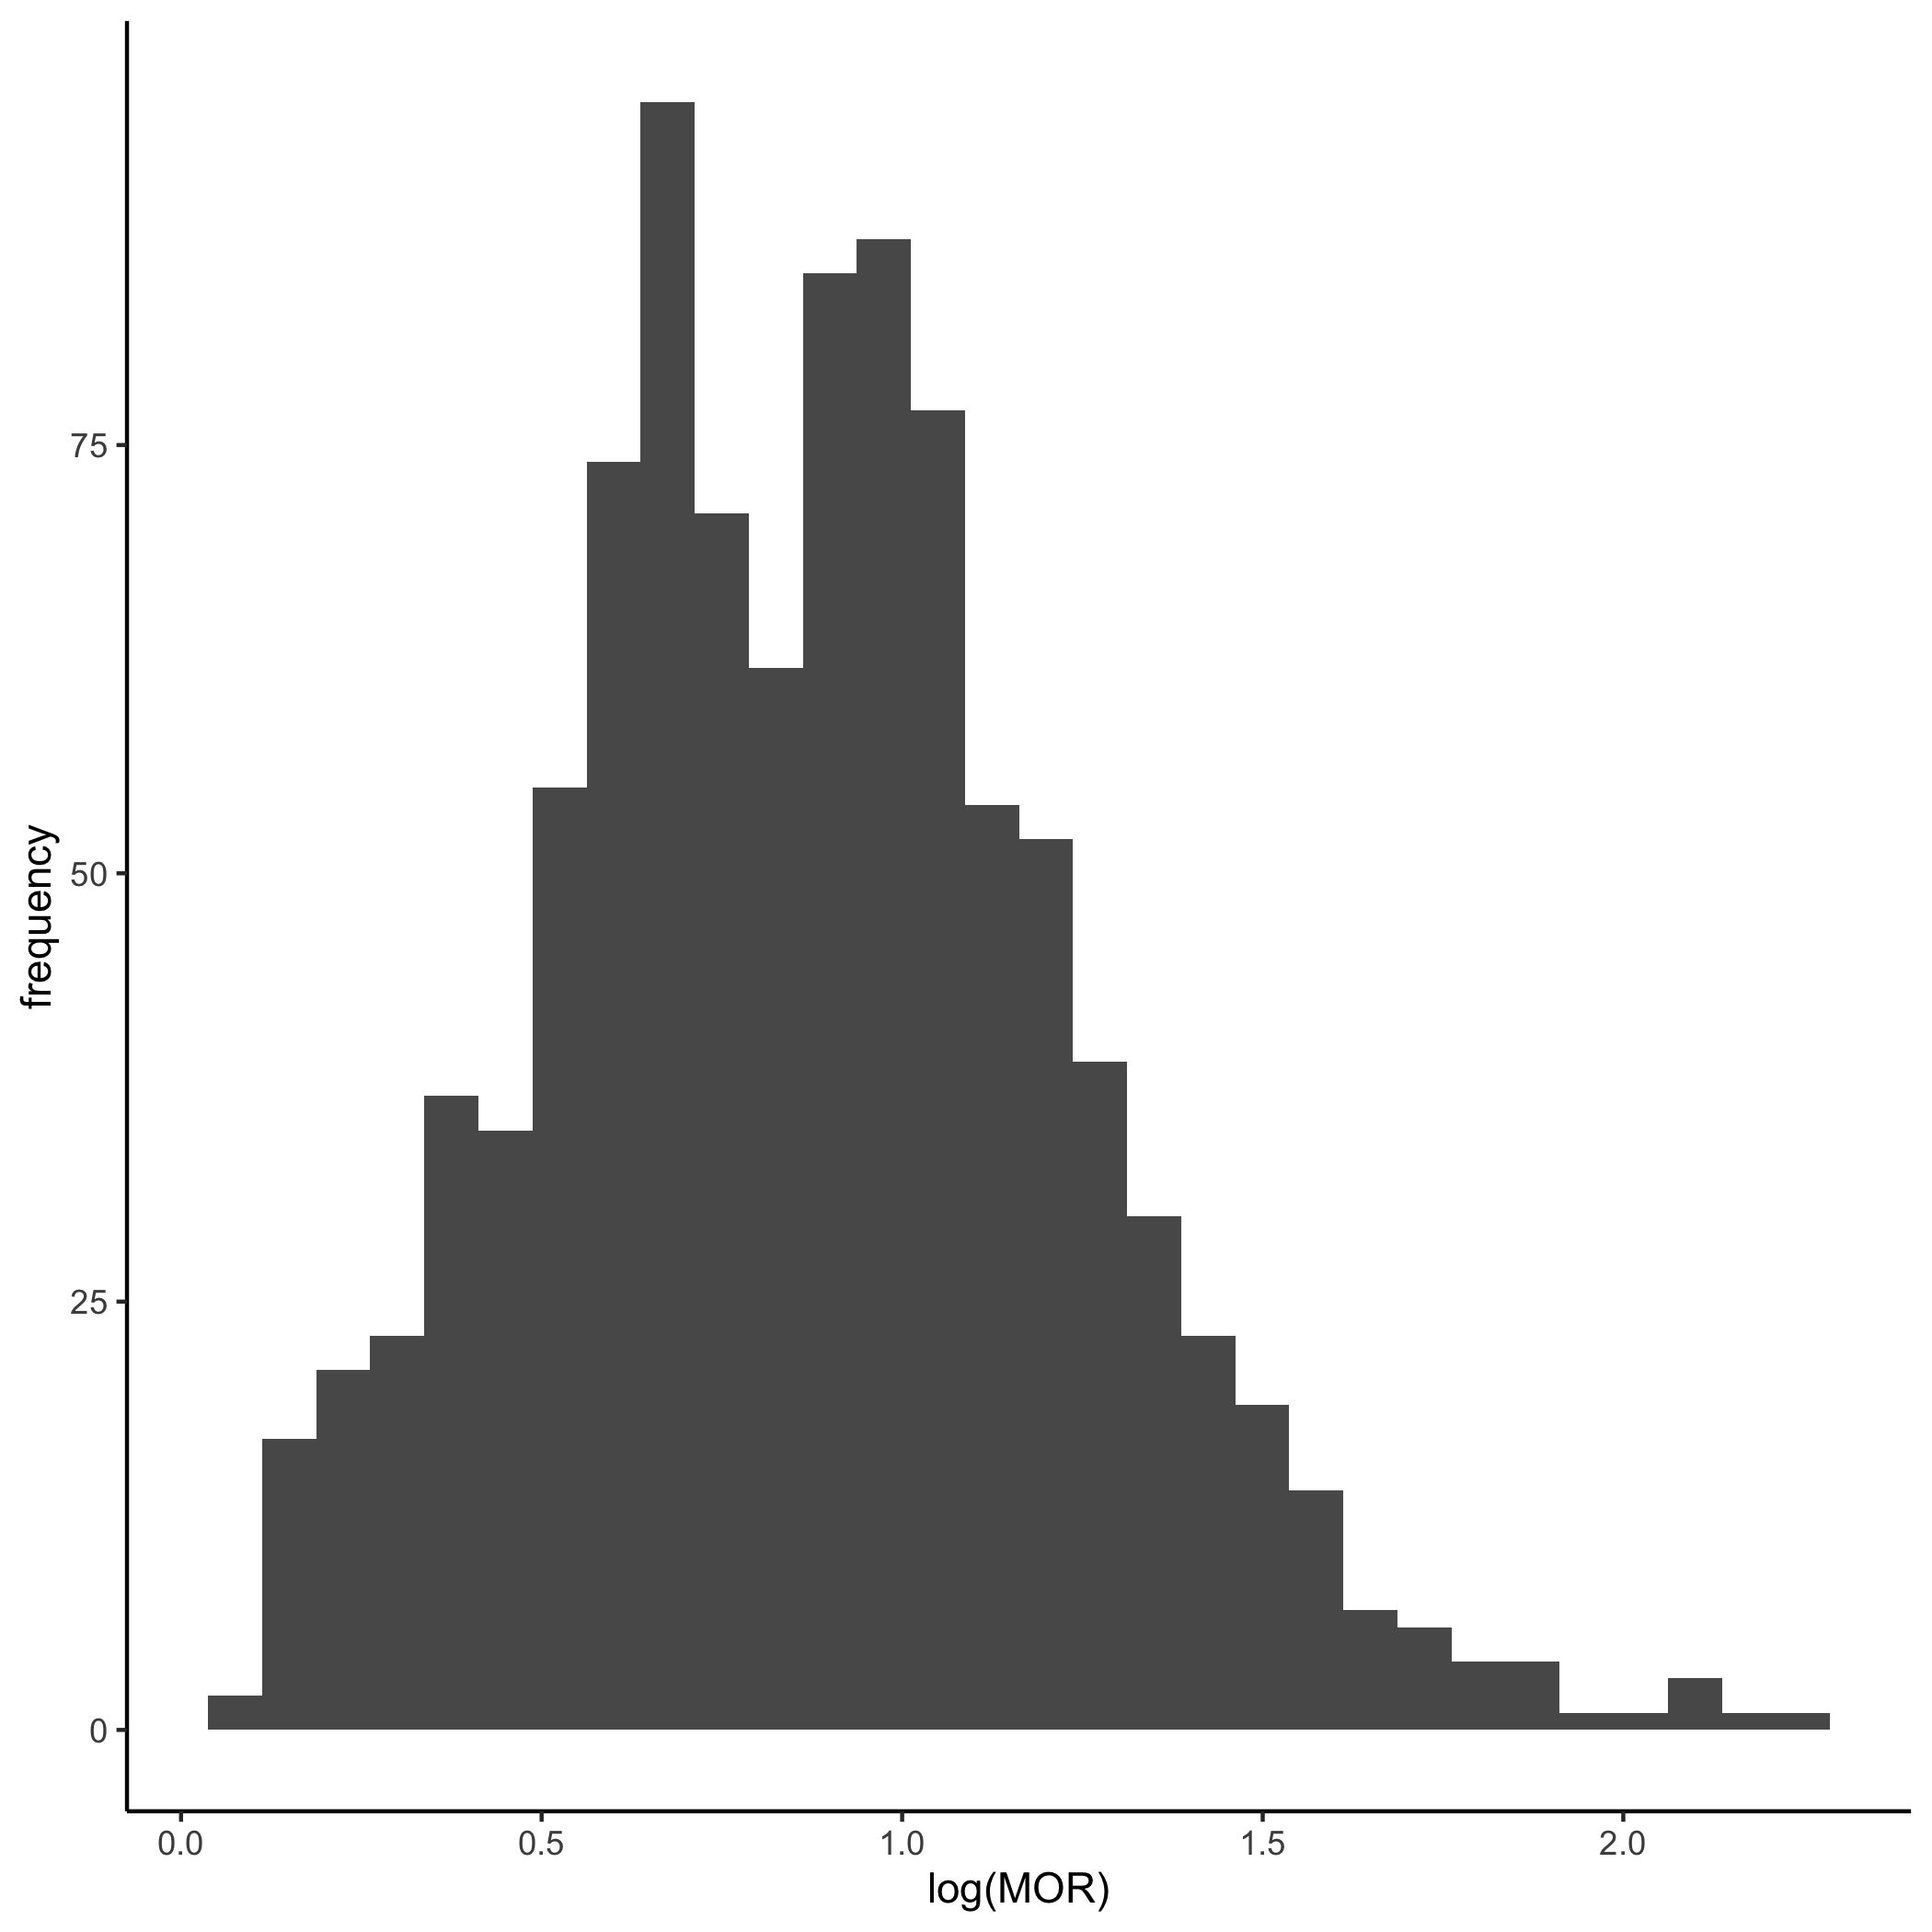
\includegraphics{../../plots/two-lvl-ran-slope/high-prev/hist_10_30_two_lvl_slp_high_prev_q3.png}

}

\caption{Cluster size 30}

}

\end{minipage}%
%
\begin{minipage}[t]{0.24\linewidth}

{\centering 

\raisebox{-\height}{

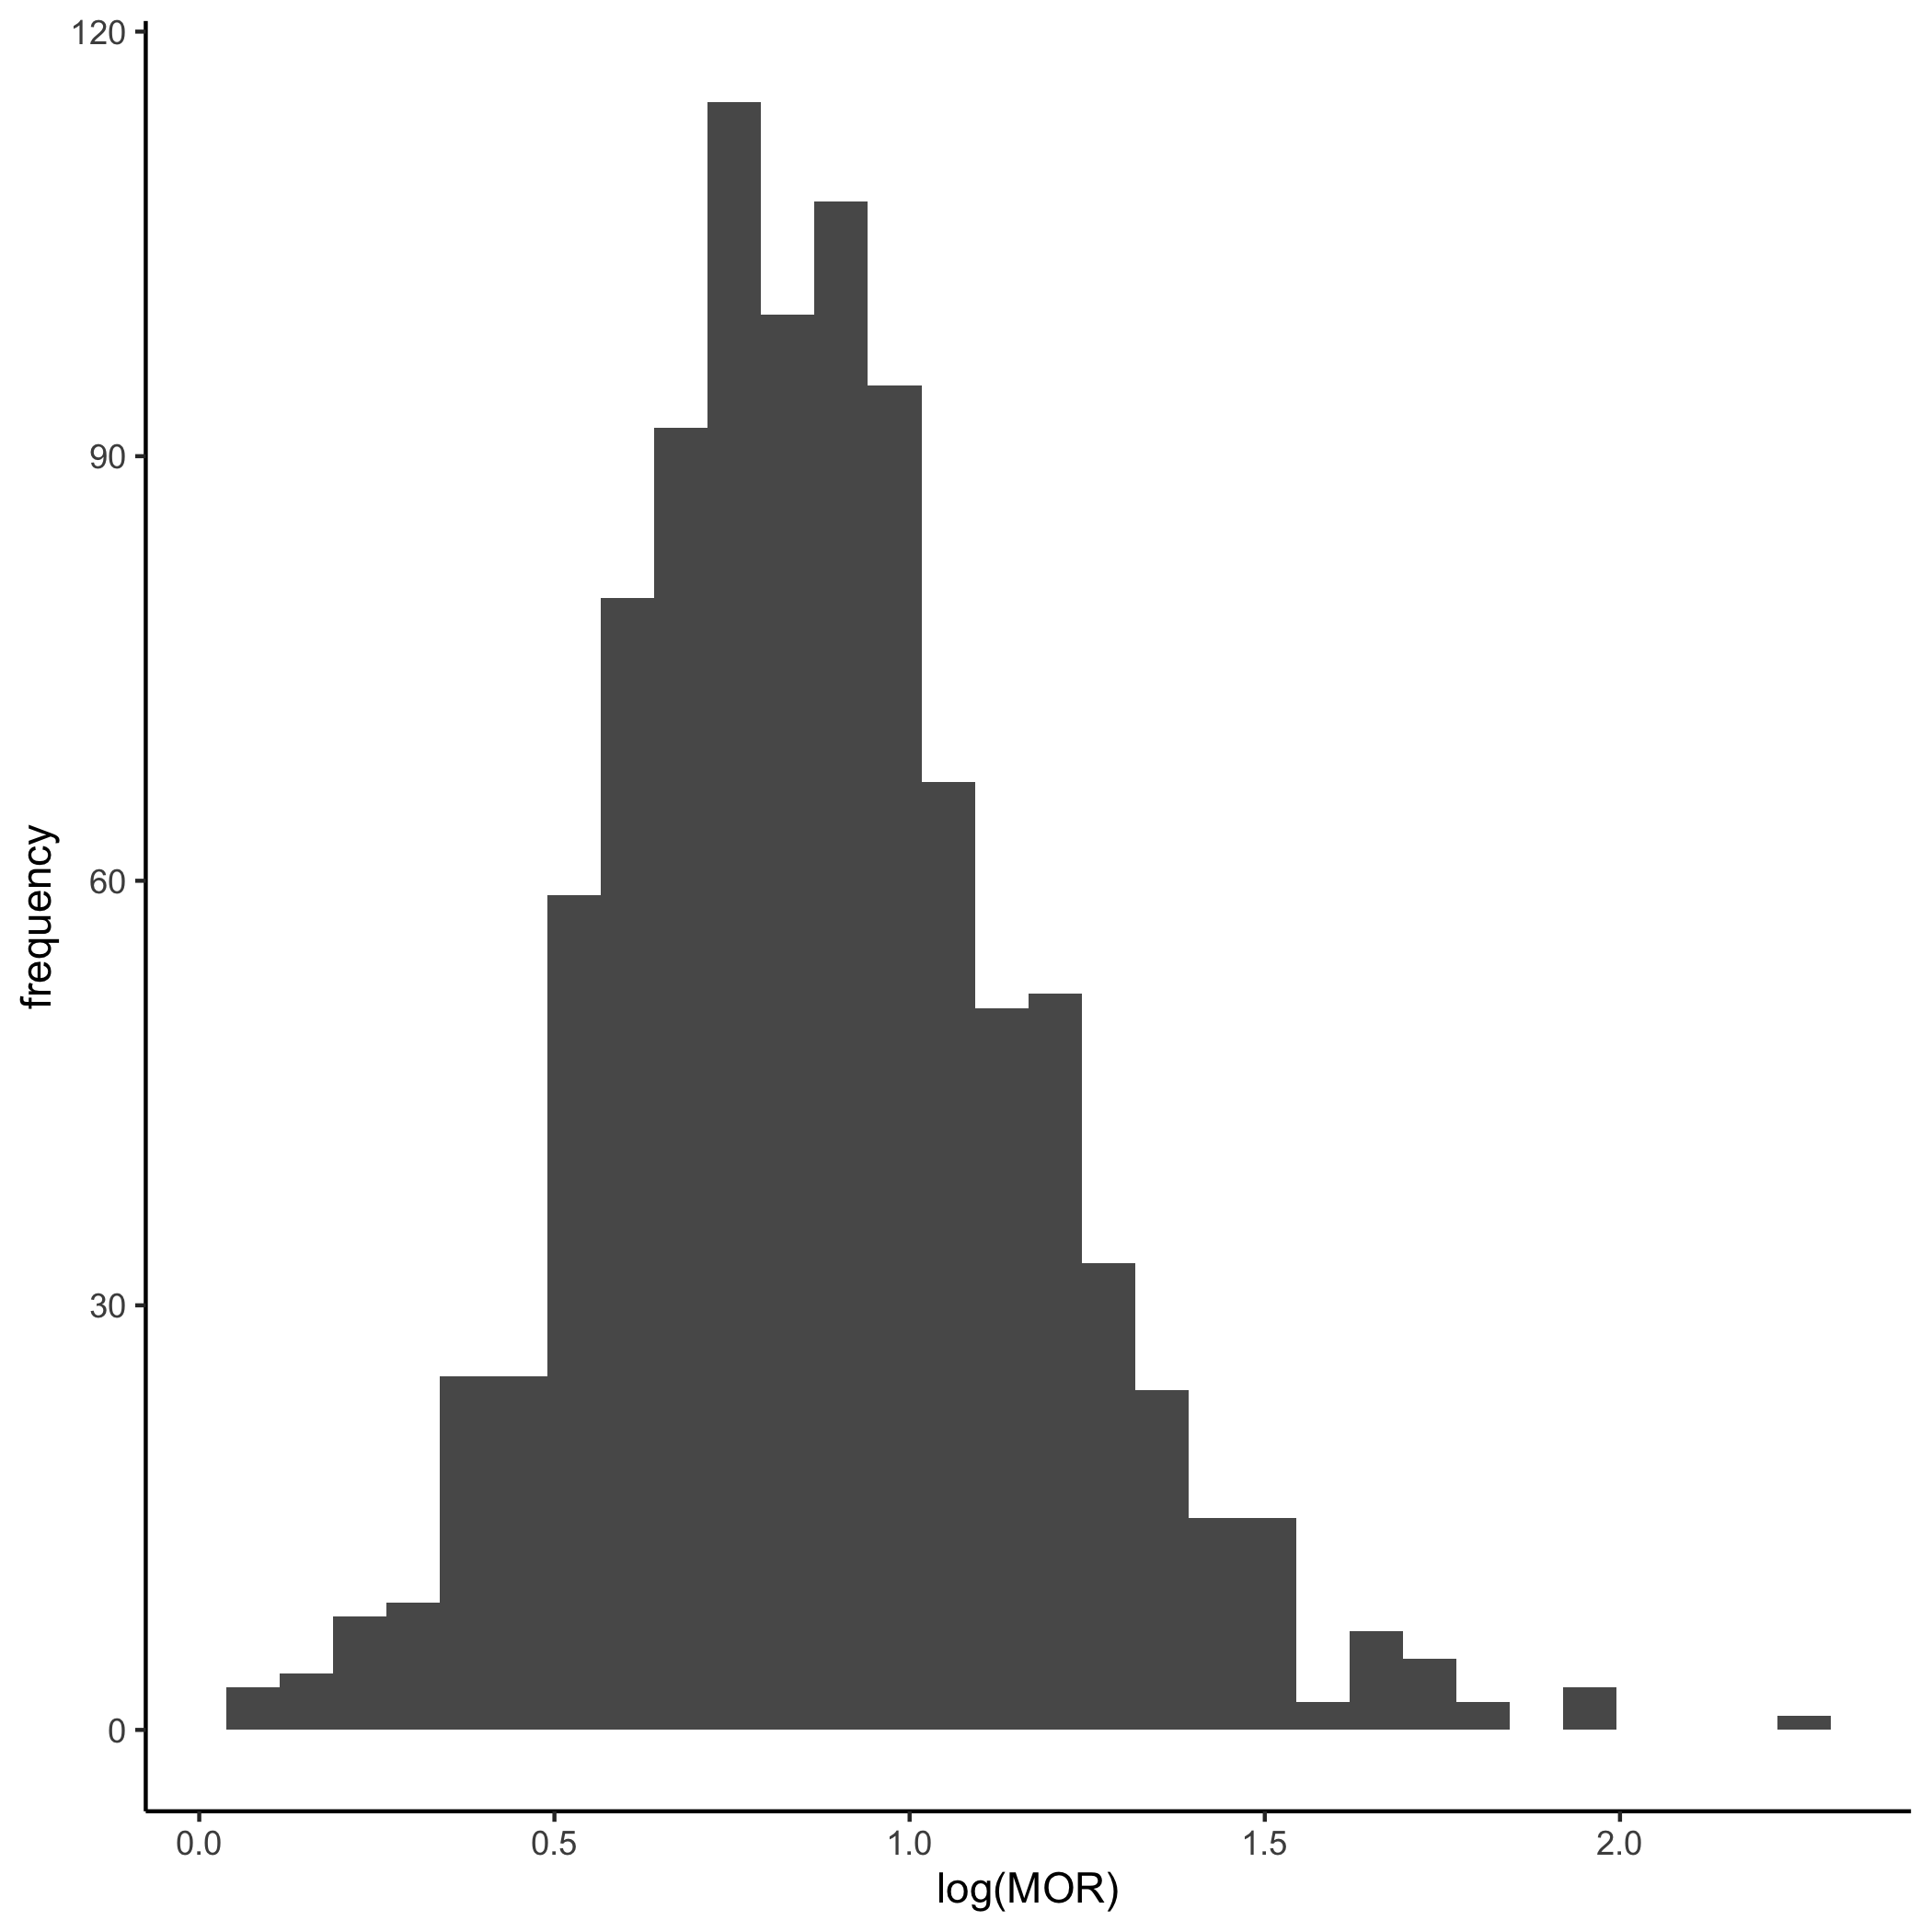
\includegraphics{../../plots/two-lvl-ran-slope/high-prev/hist_10_50_two_lvl_slp_high_prev_q3.png}

}

\caption{Cluster size 50}

}

\end{minipage}%
\newline
\begin{minipage}[t]{\linewidth}

{\centering 

~

}

\end{minipage}%
\newline
\begin{minipage}[t]{0.05\linewidth}

{\centering 

\rotatebox[origin=br]{90}{\tiny Cluster Number 30}

}

\end{minipage}%
%
\begin{minipage}[t]{0.24\linewidth}

{\centering 

\raisebox{-\height}{

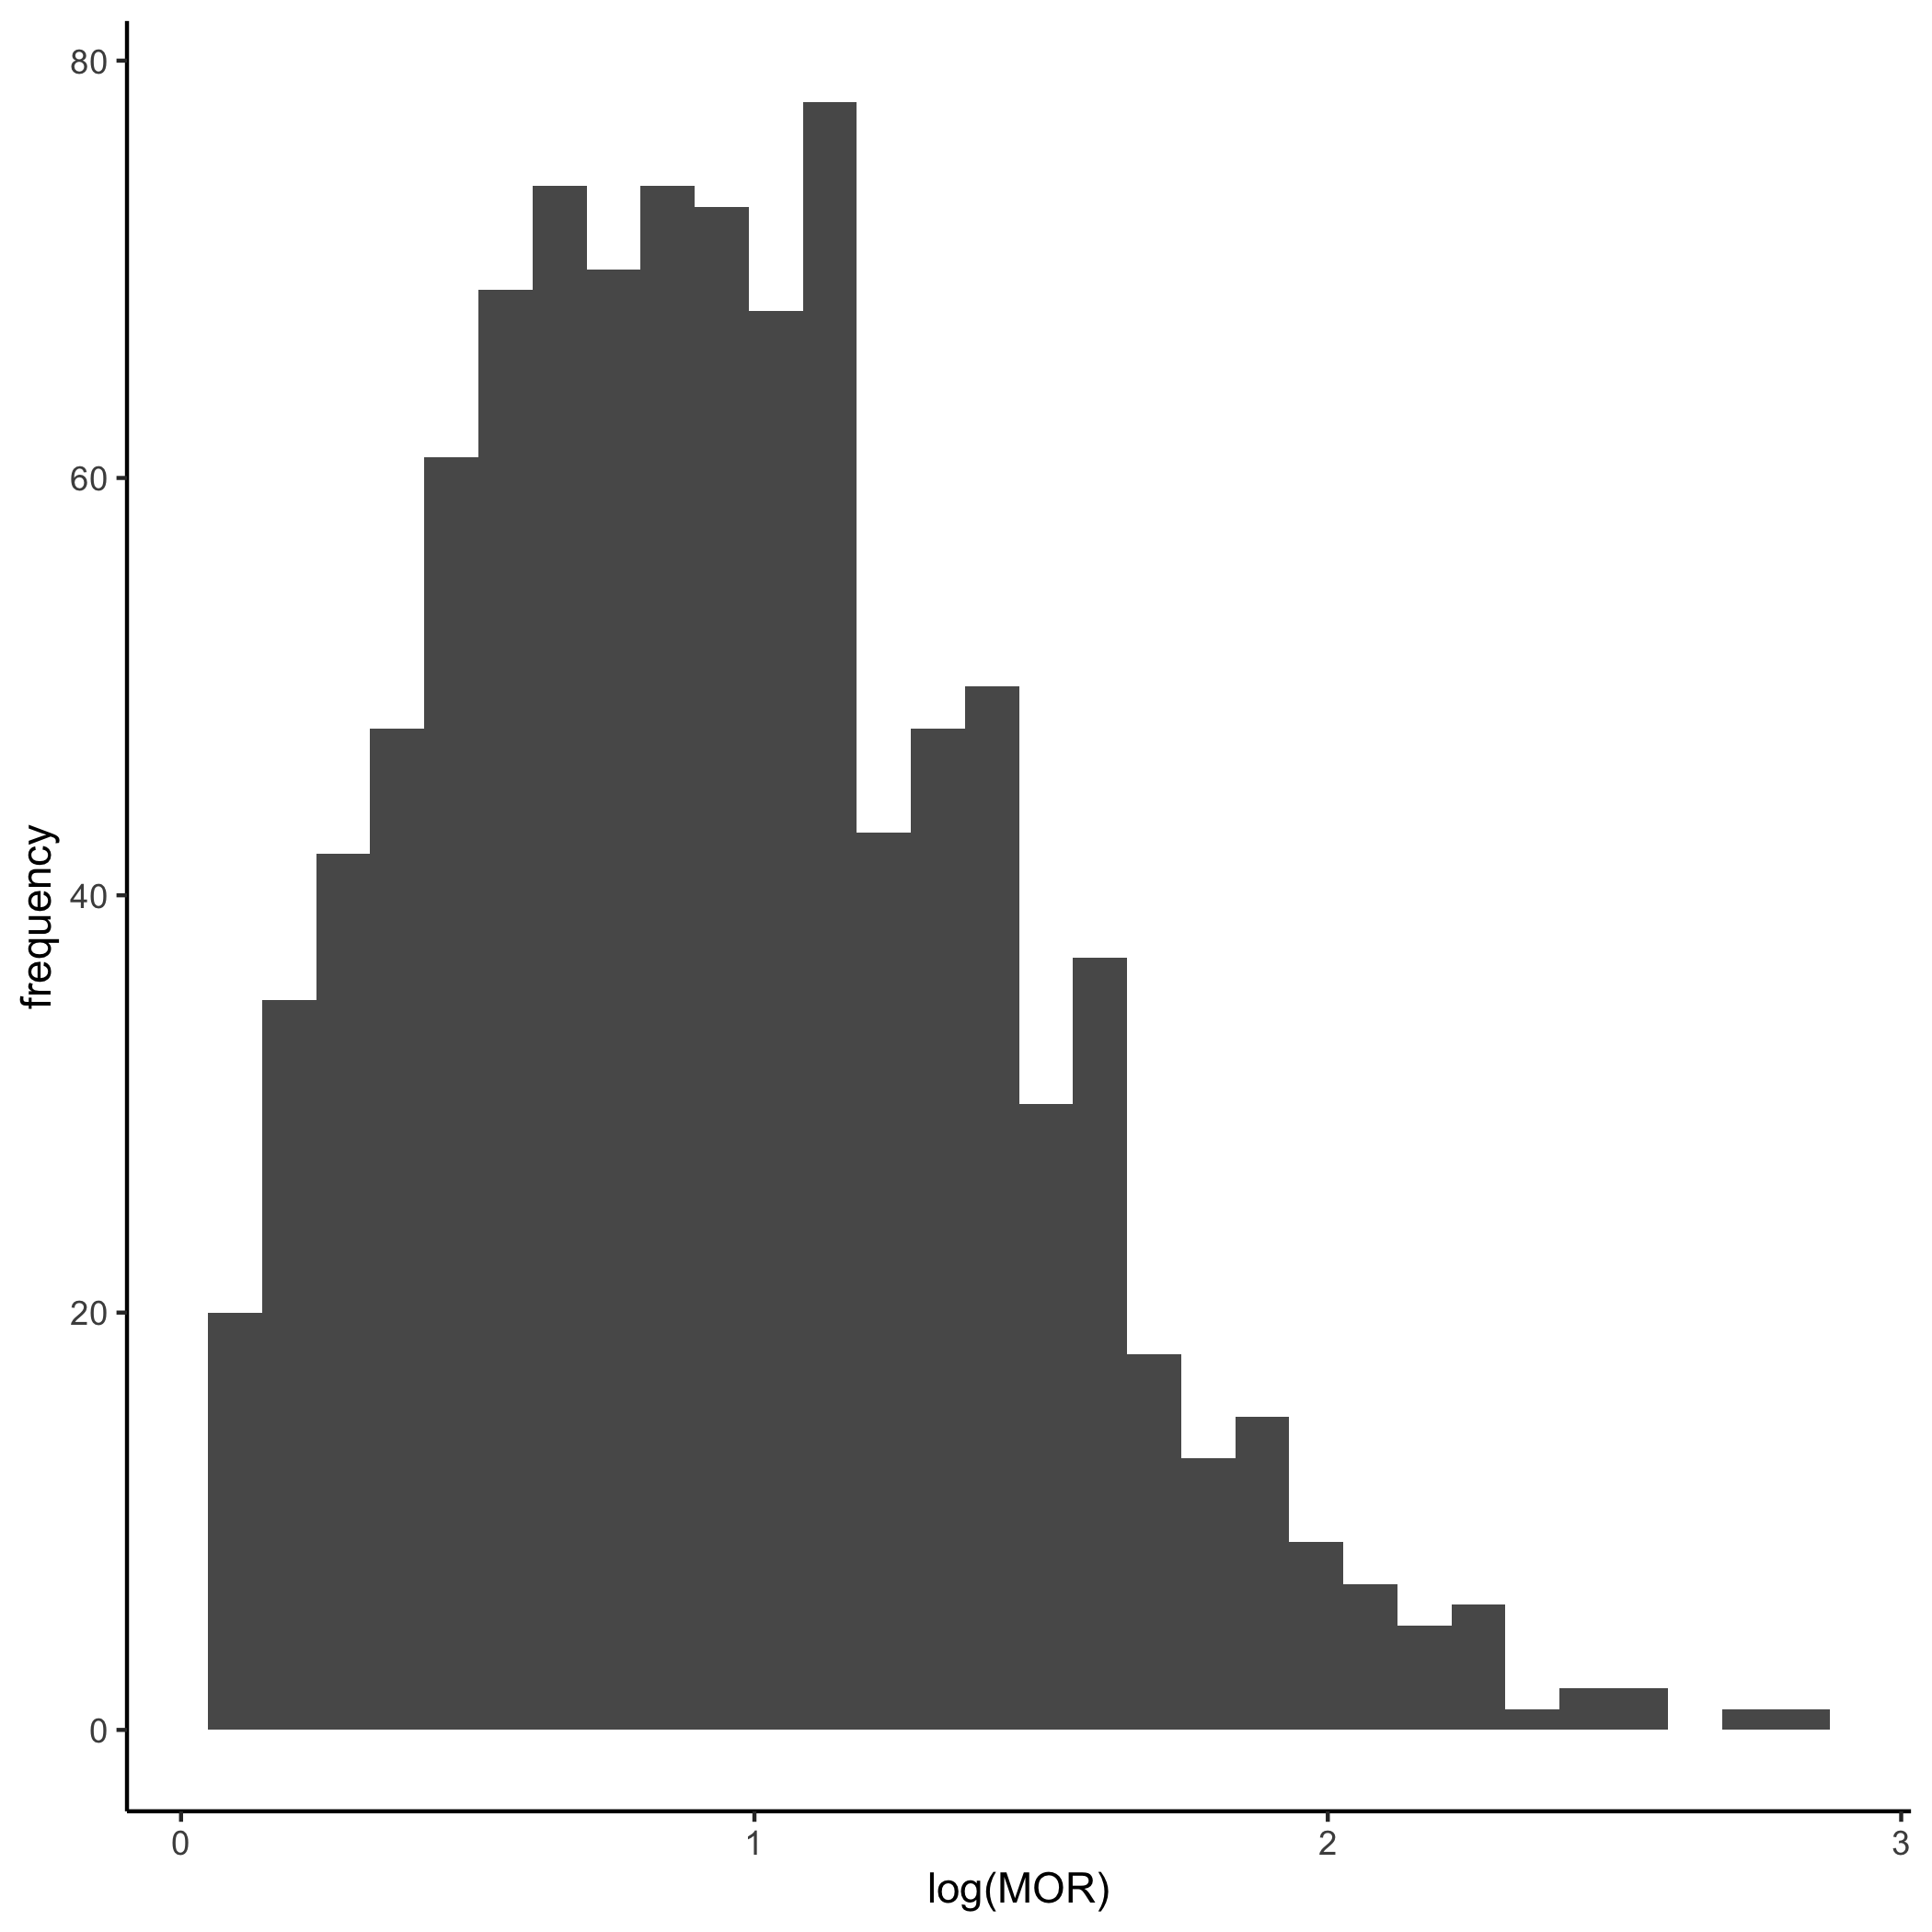
\includegraphics{../../plots/two-lvl-ran-slope/high-prev/hist_30_5_two_lvl_slp_high_prev_q3.png}

}

\caption{Cluster size 5}

}

\end{minipage}%
%
\begin{minipage}[t]{0.24\linewidth}

{\centering 

\raisebox{-\height}{

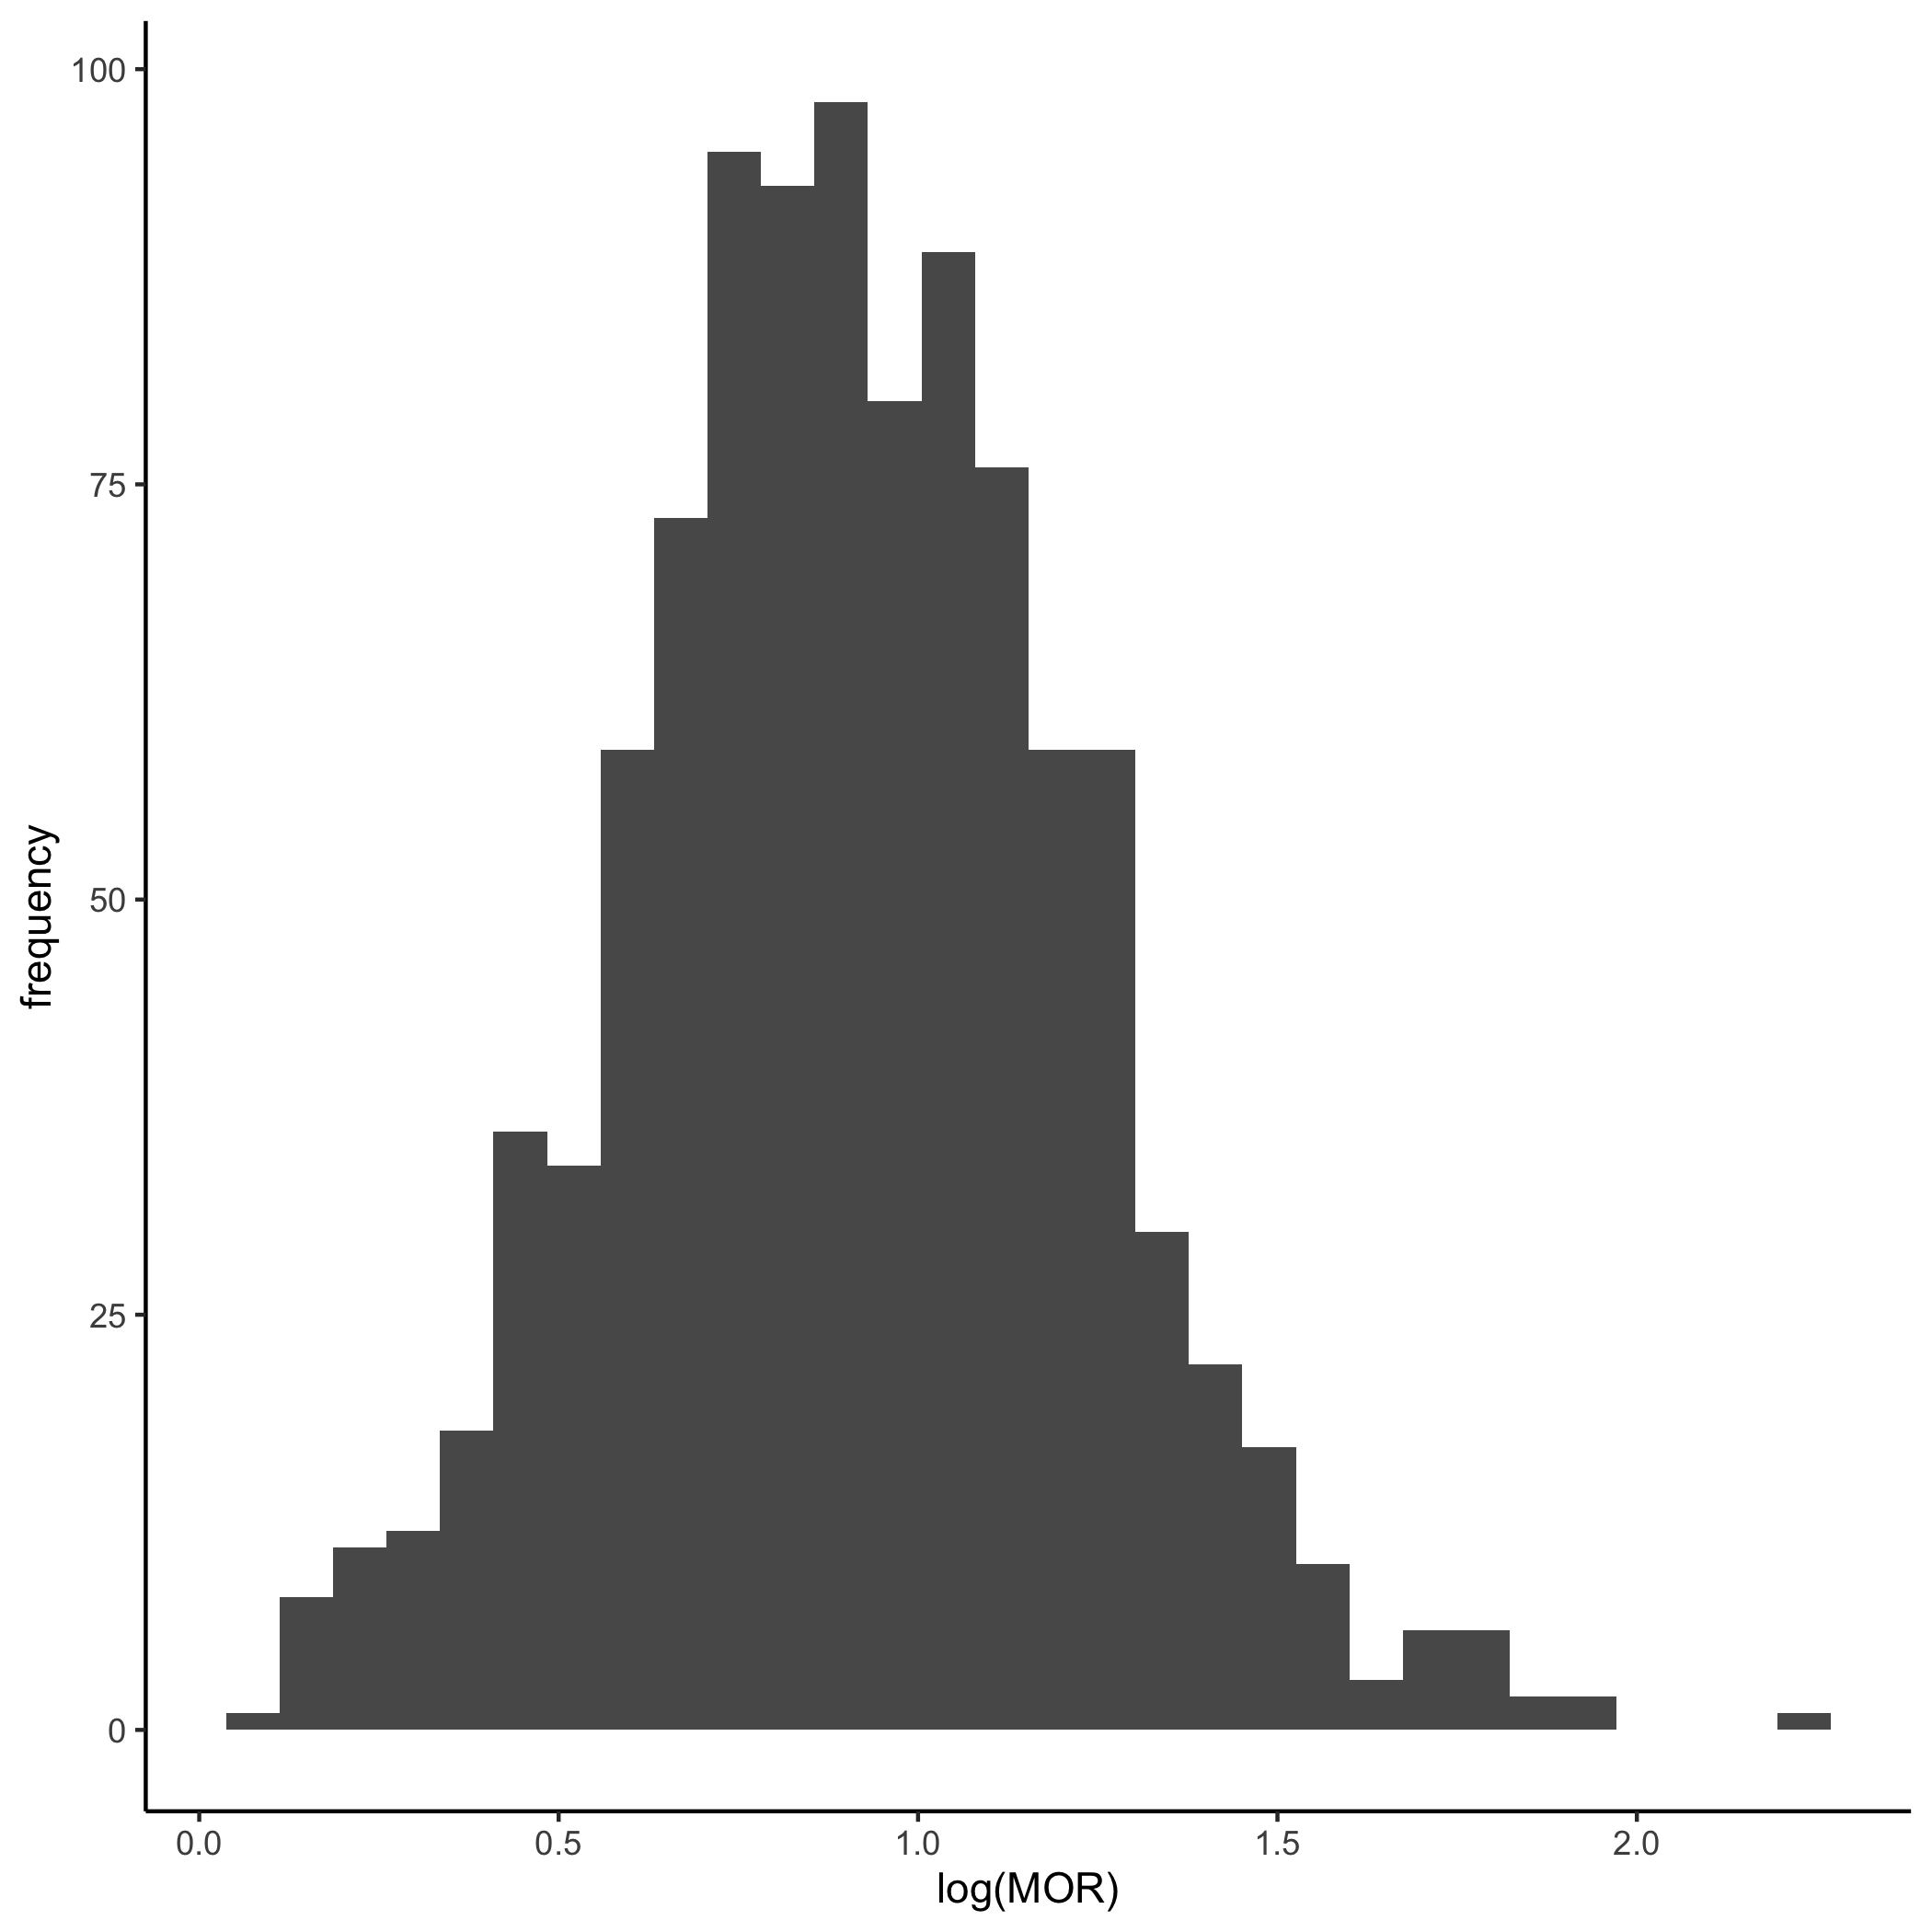
\includegraphics{../../plots/two-lvl-ran-slope/high-prev/hist_30_10_two_lvl_slp_high_prev_q3.png}

}

\caption{Cluster size 10}

}

\end{minipage}%
%
\begin{minipage}[t]{0.24\linewidth}

{\centering 

\raisebox{-\height}{

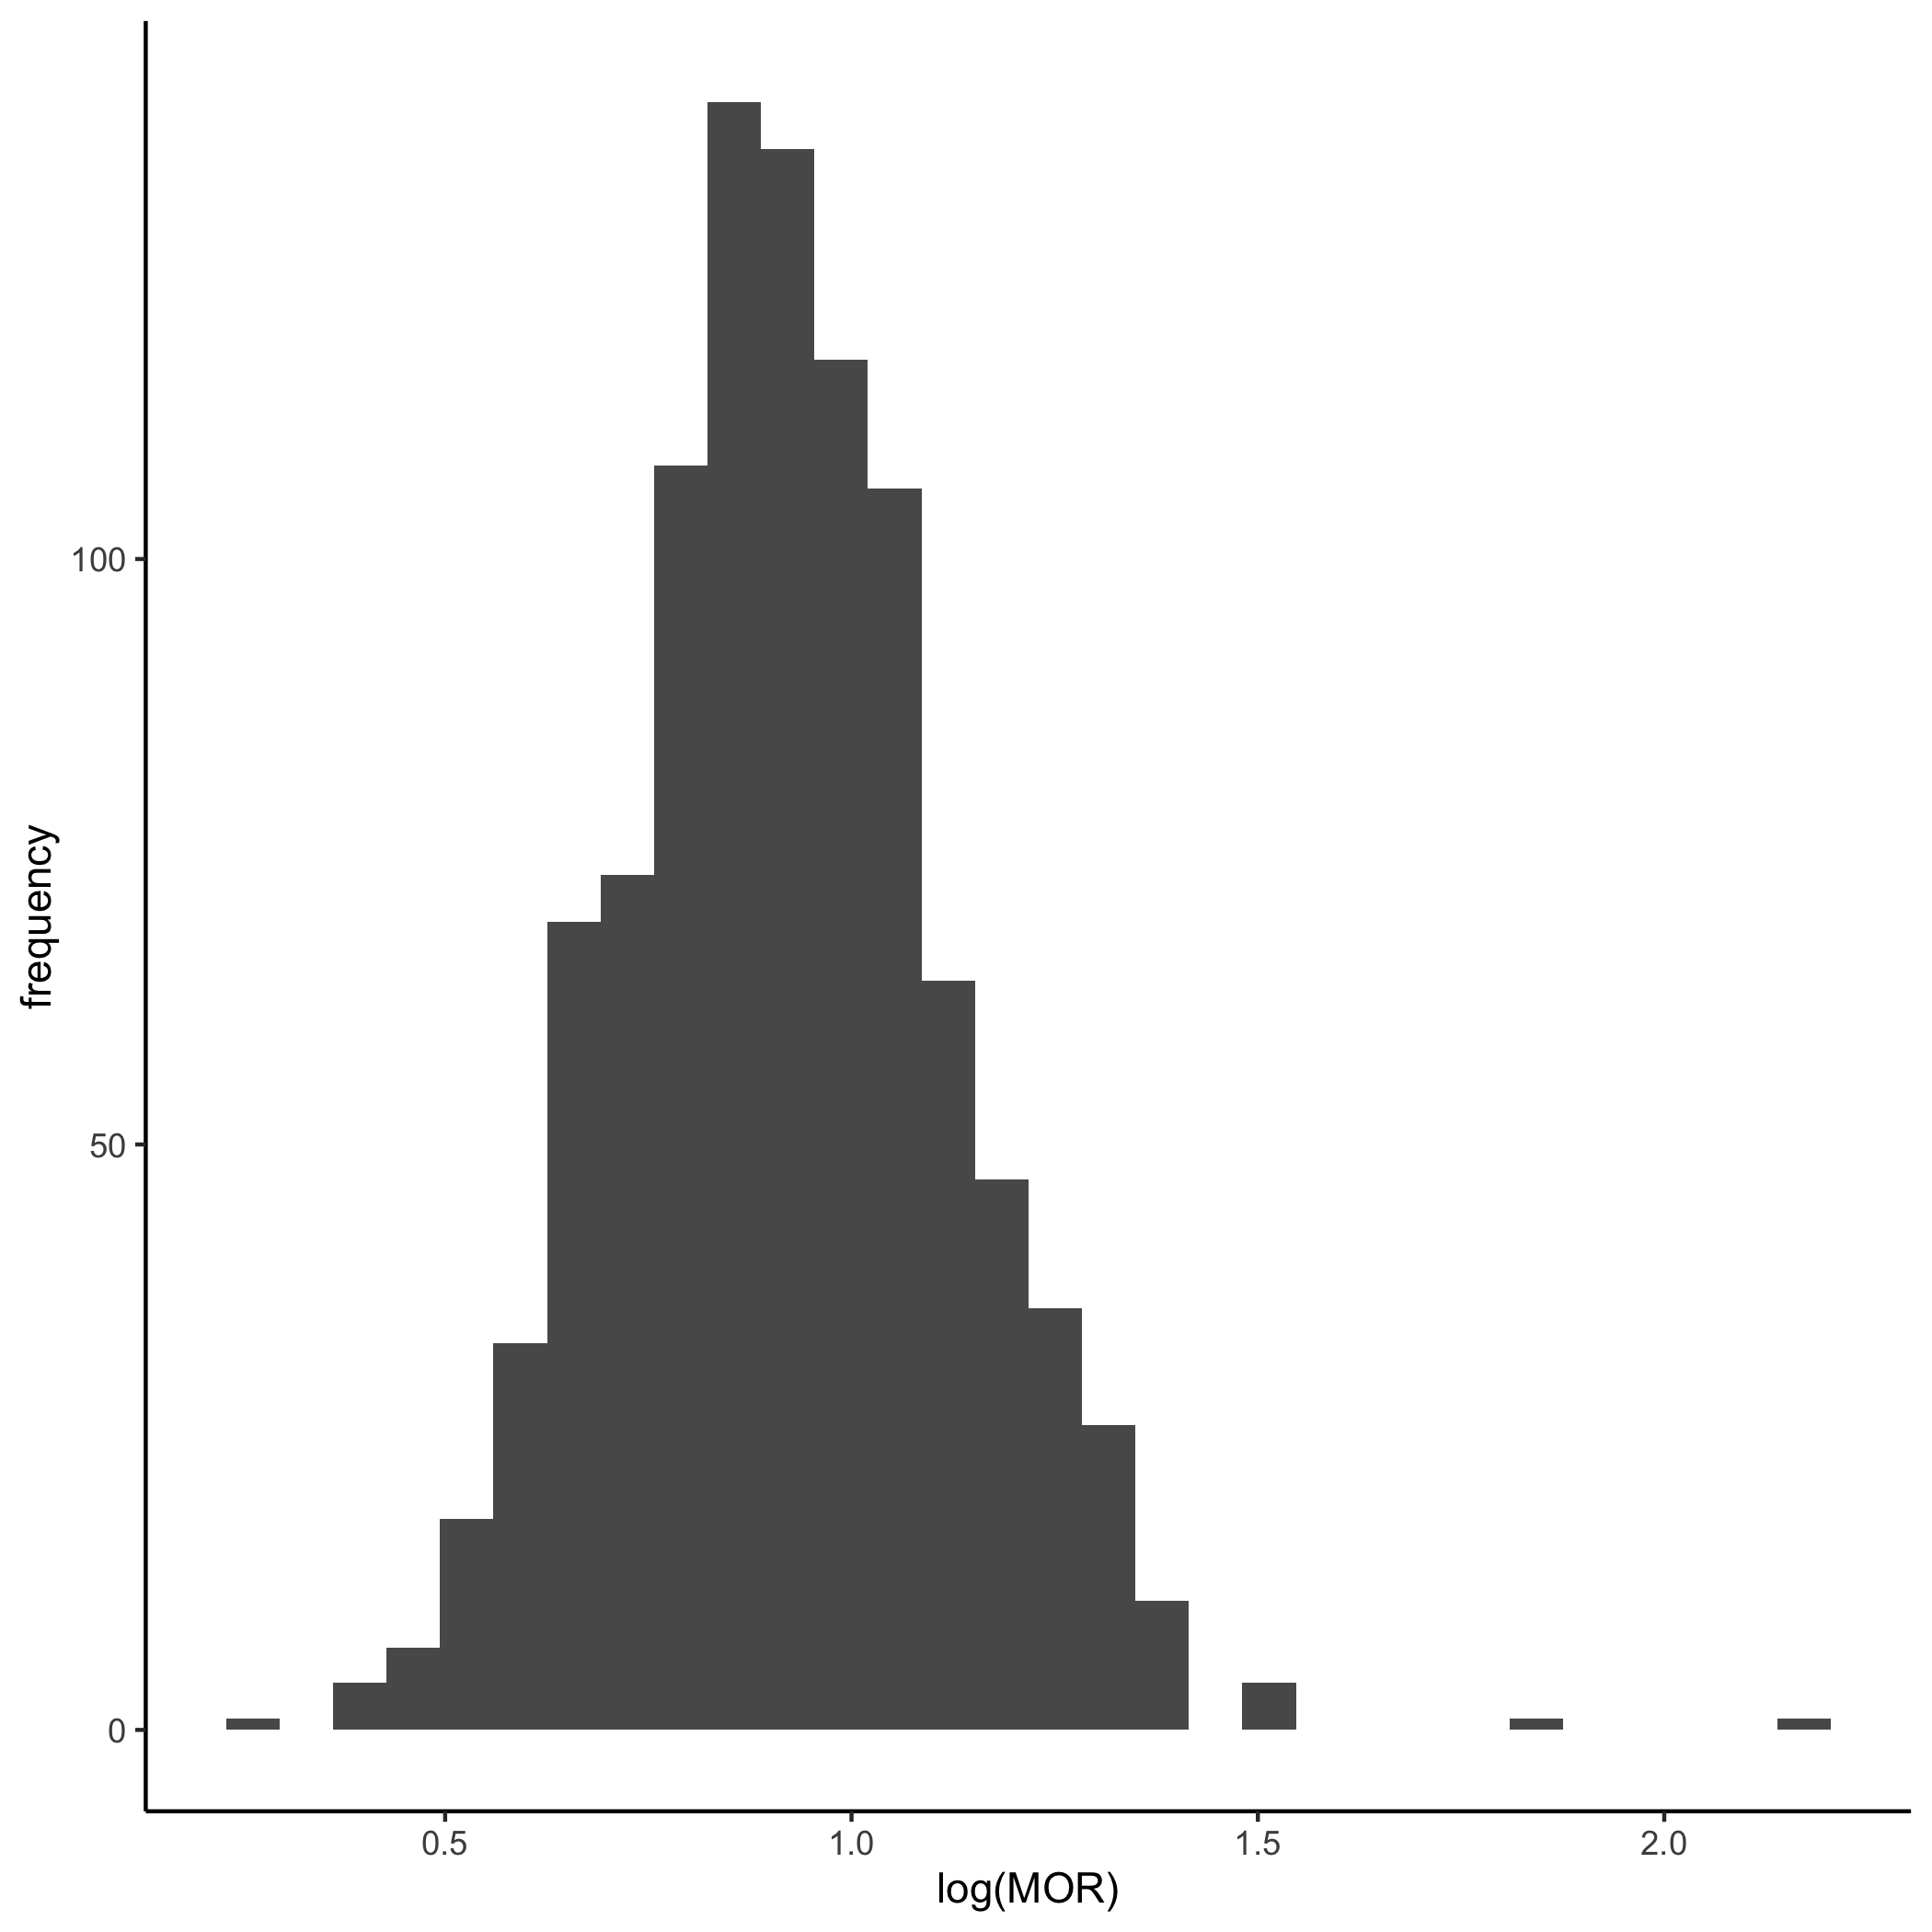
\includegraphics{../../plots/two-lvl-ran-slope/high-prev/hist_30_30_two_lvl_slp_high_prev_q3.png}

}

\caption{Cluster size 30}

}

\end{minipage}%
%
\begin{minipage}[t]{0.24\linewidth}

{\centering 

\raisebox{-\height}{

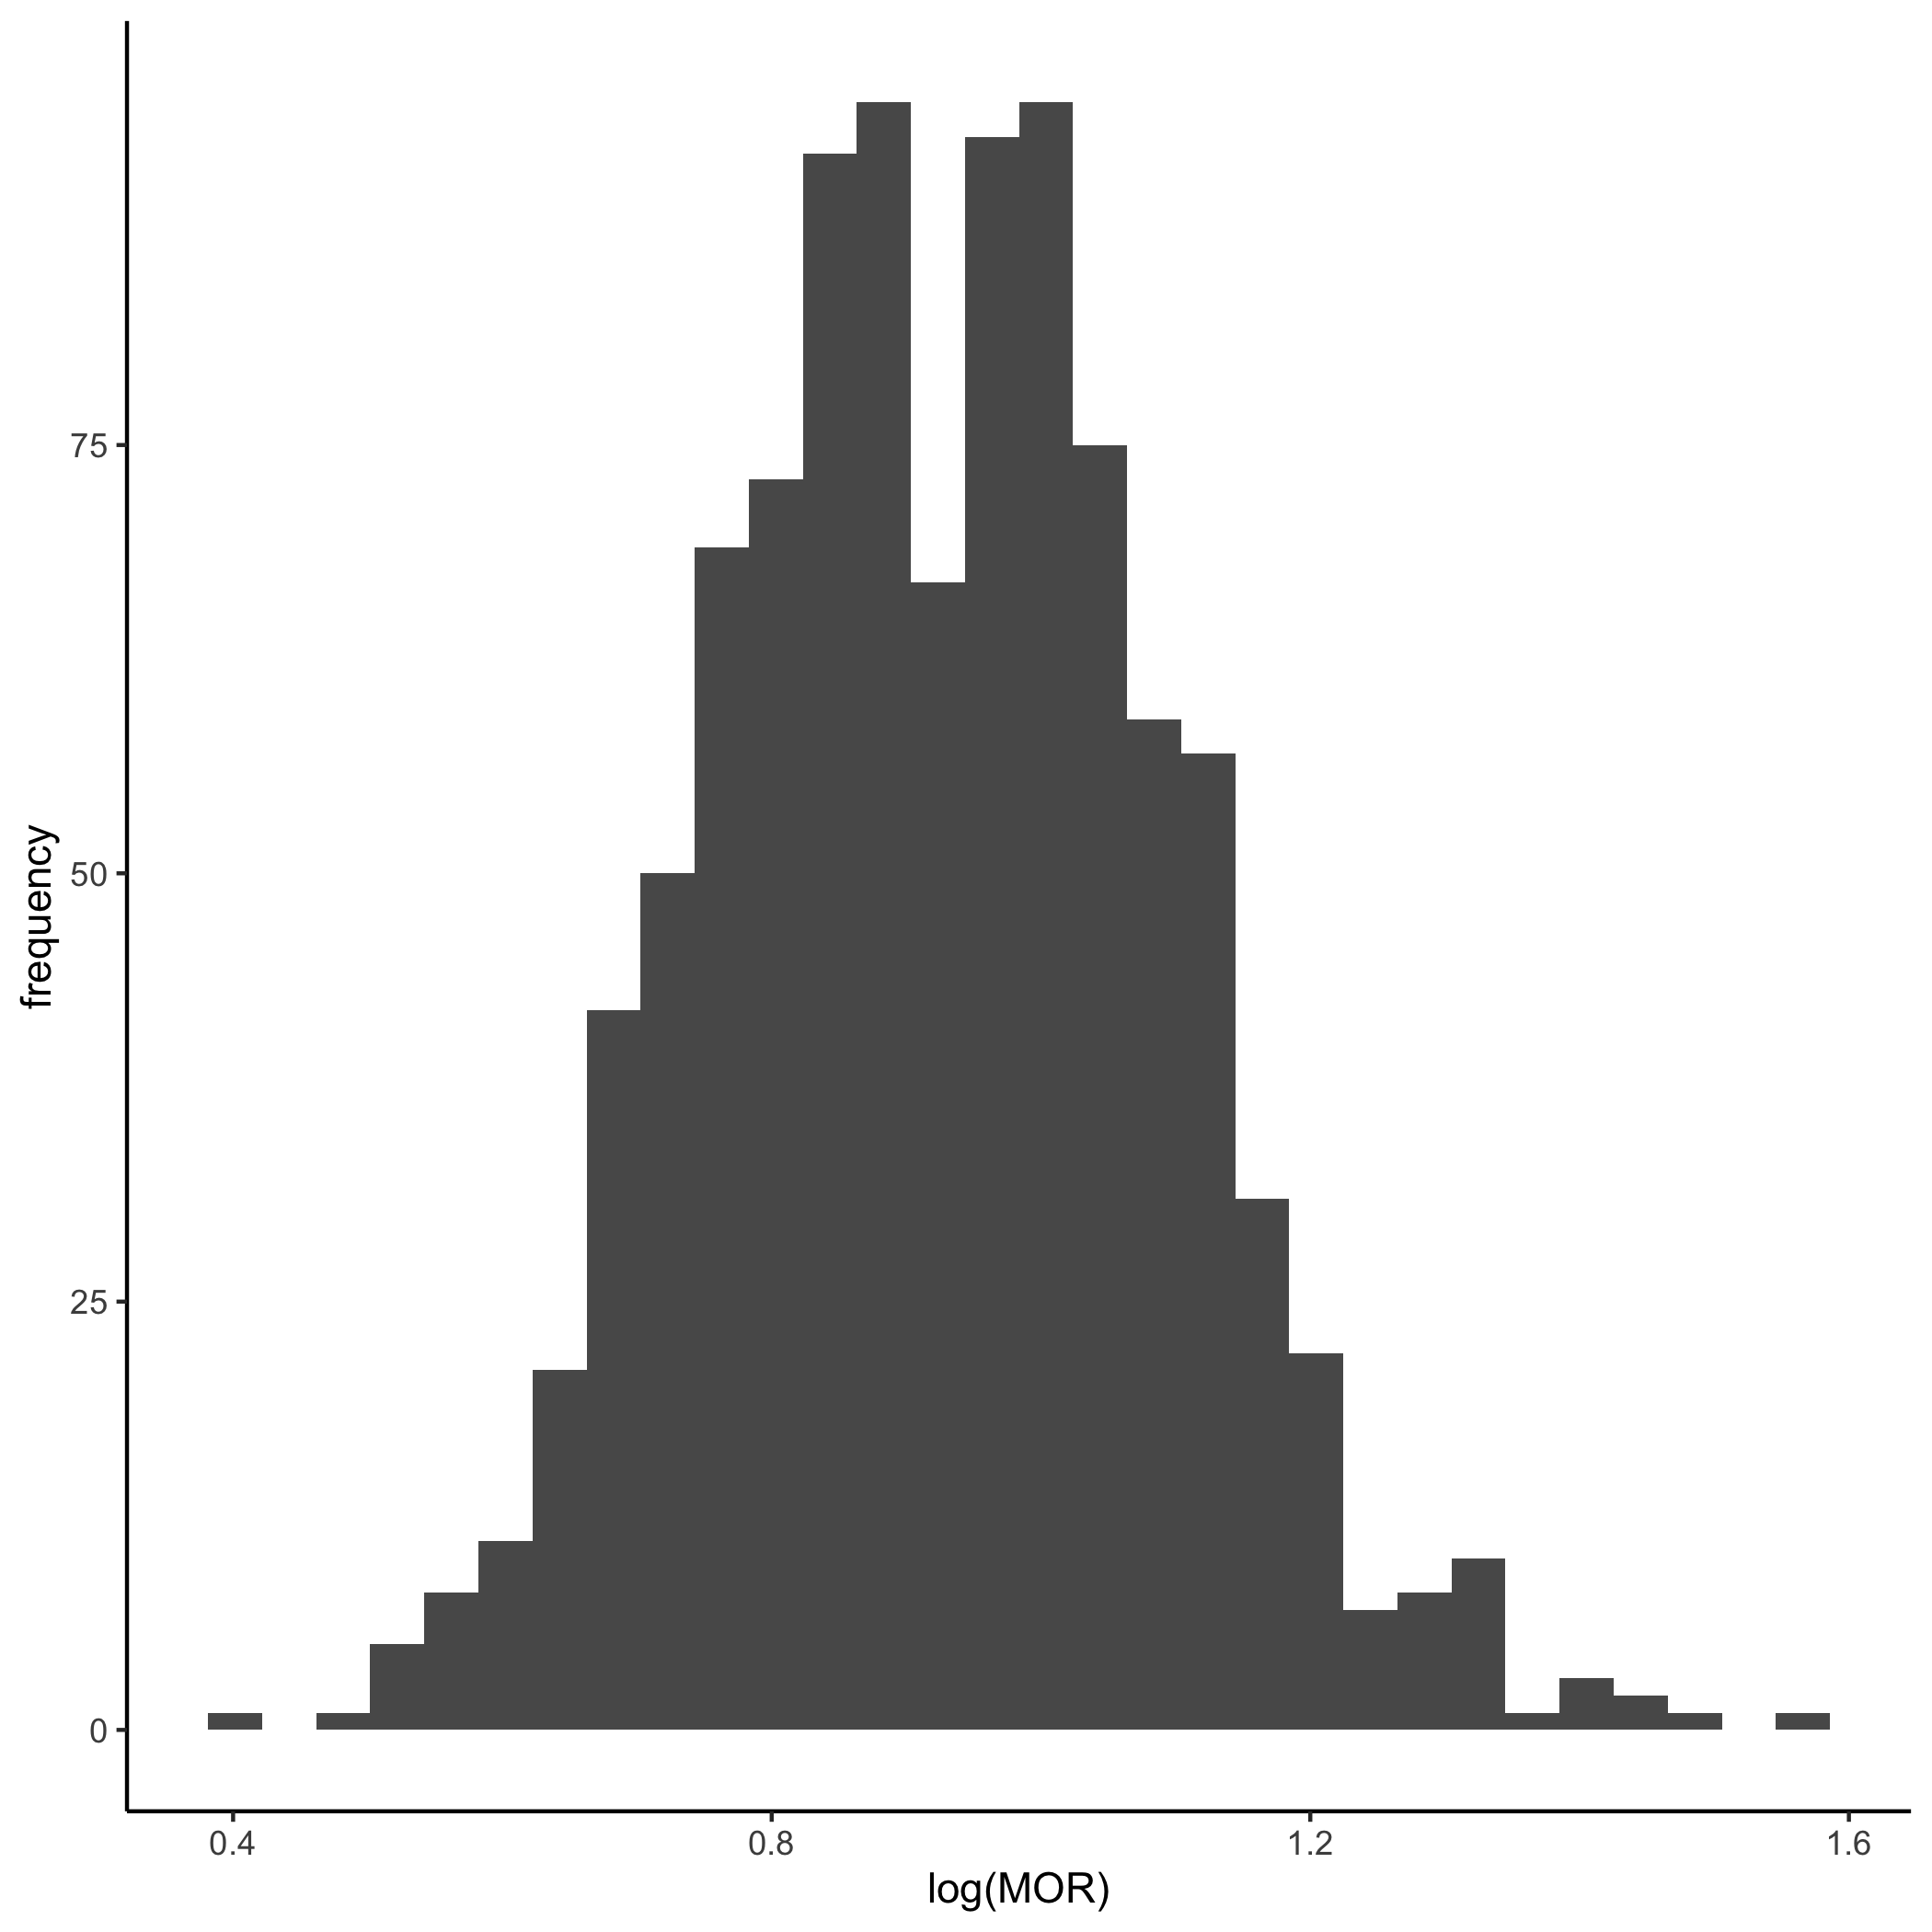
\includegraphics{../../plots/two-lvl-ran-slope/high-prev/hist_30_50_two_lvl_slp_high_prev_q3.png}

}

\caption{Cluster size 50}

}

\end{minipage}%
\newline
\begin{minipage}[t]{\linewidth}

{\centering 

~

}

\end{minipage}%
\newline
\begin{minipage}[t]{0.05\linewidth}

{\centering 

\rotatebox[origin=br]{90}{\tiny Cluster Number 50}

}

\end{minipage}%
%
\begin{minipage}[t]{0.24\linewidth}

{\centering 

\raisebox{-\height}{

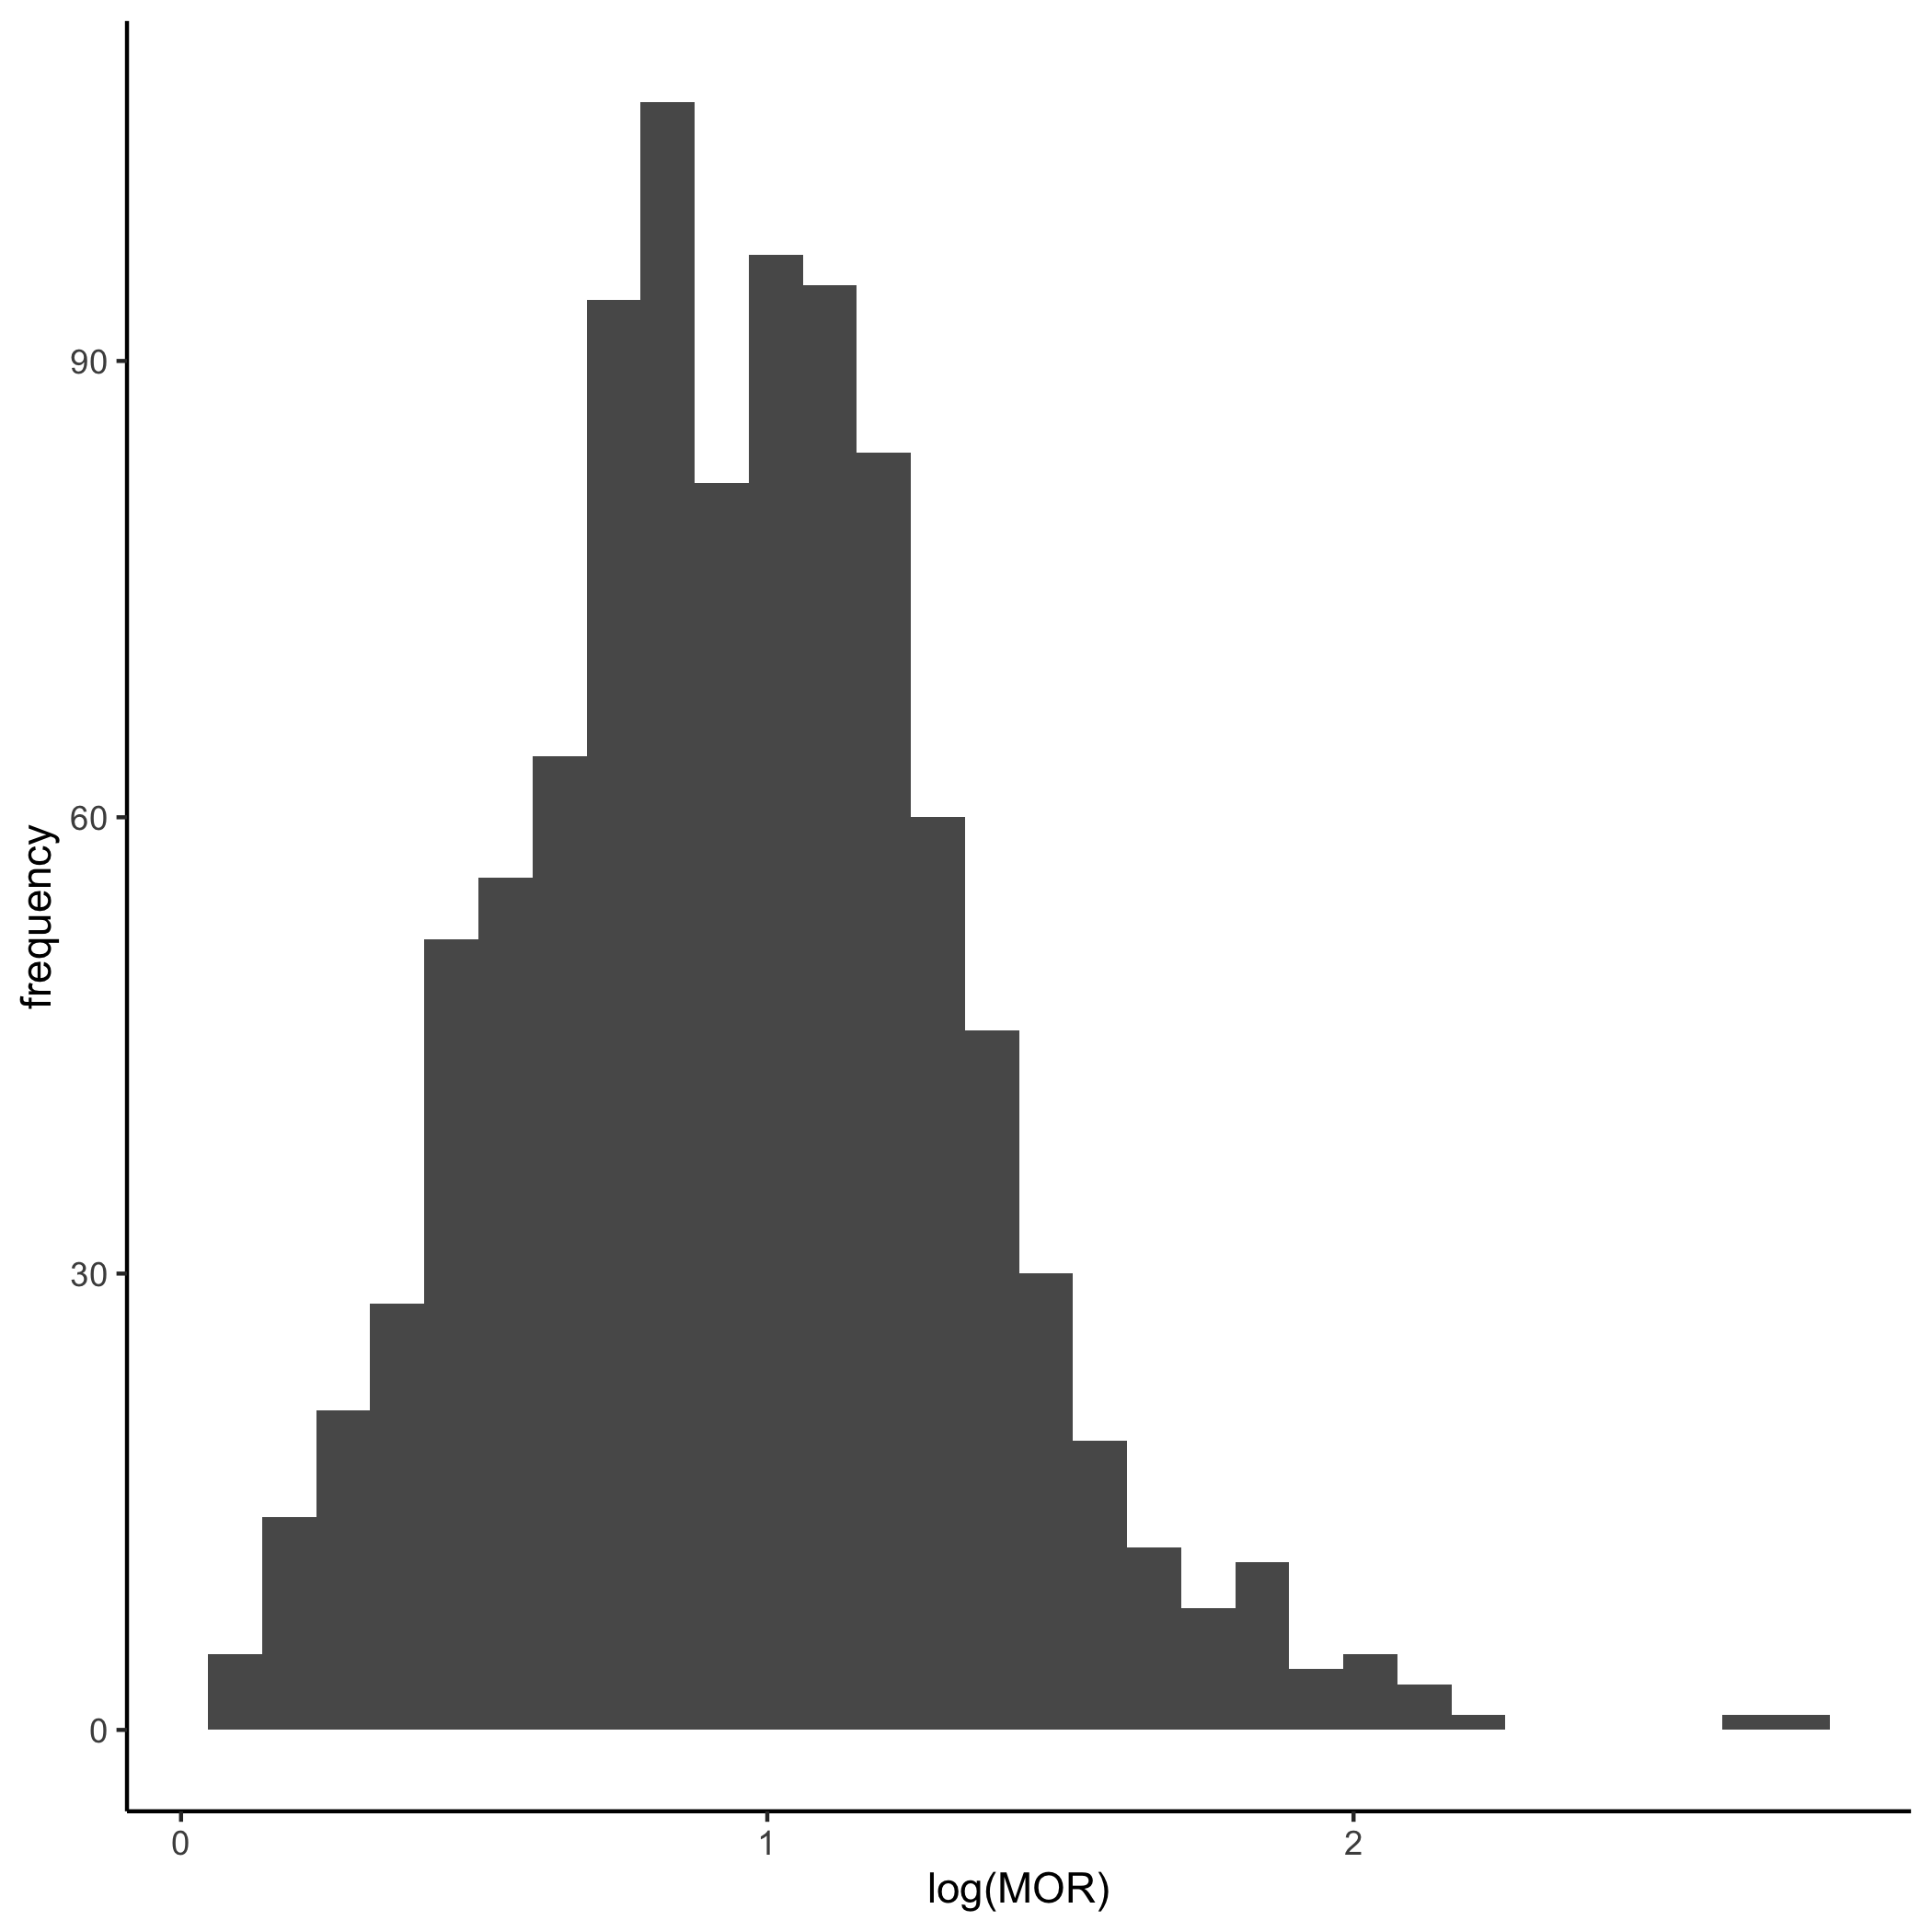
\includegraphics{../../plots/two-lvl-ran-slope/high-prev/hist_50_5_two_lvl_slp_high_prev_q3.png}

}

\caption{Cluster size 5}

}

\end{minipage}%
%
\begin{minipage}[t]{0.24\linewidth}

{\centering 

\raisebox{-\height}{

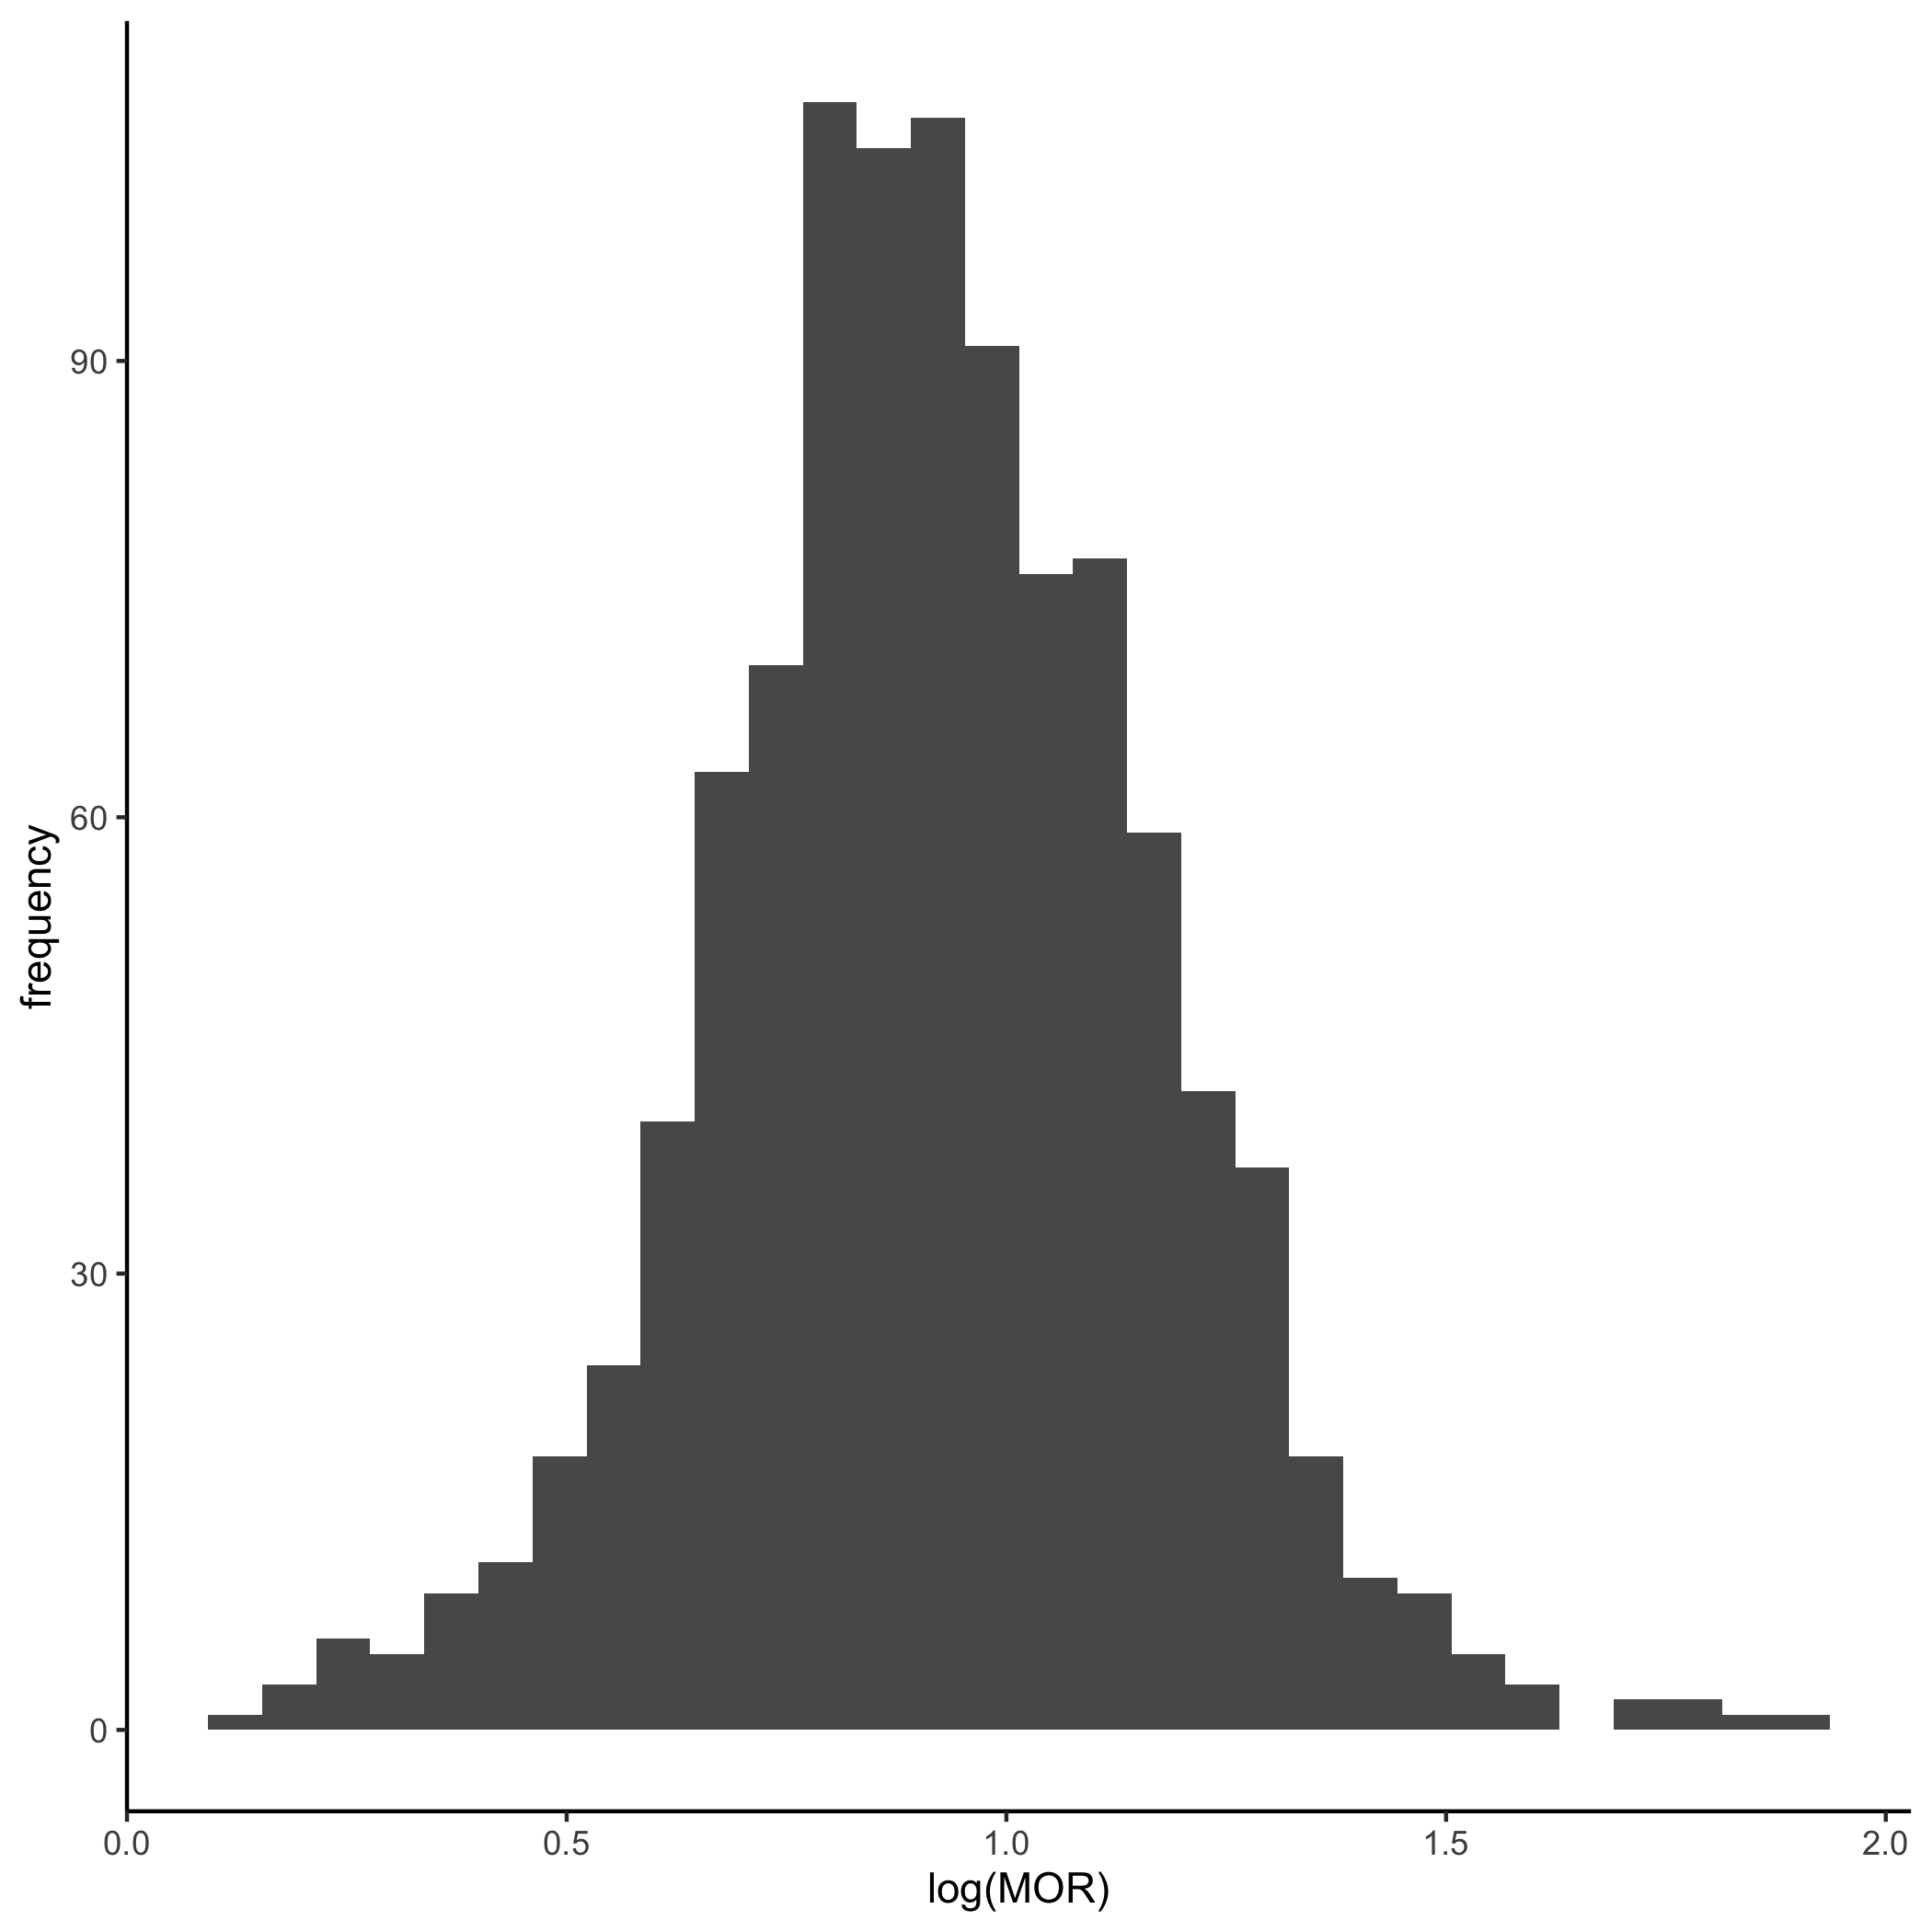
\includegraphics{../../plots/two-lvl-ran-slope/high-prev/hist_50_10_two_lvl_slp_high_prev_q3.png}

}

\caption{Cluster size 10}

}

\end{minipage}%
%
\begin{minipage}[t]{0.24\linewidth}

{\centering 

\raisebox{-\height}{

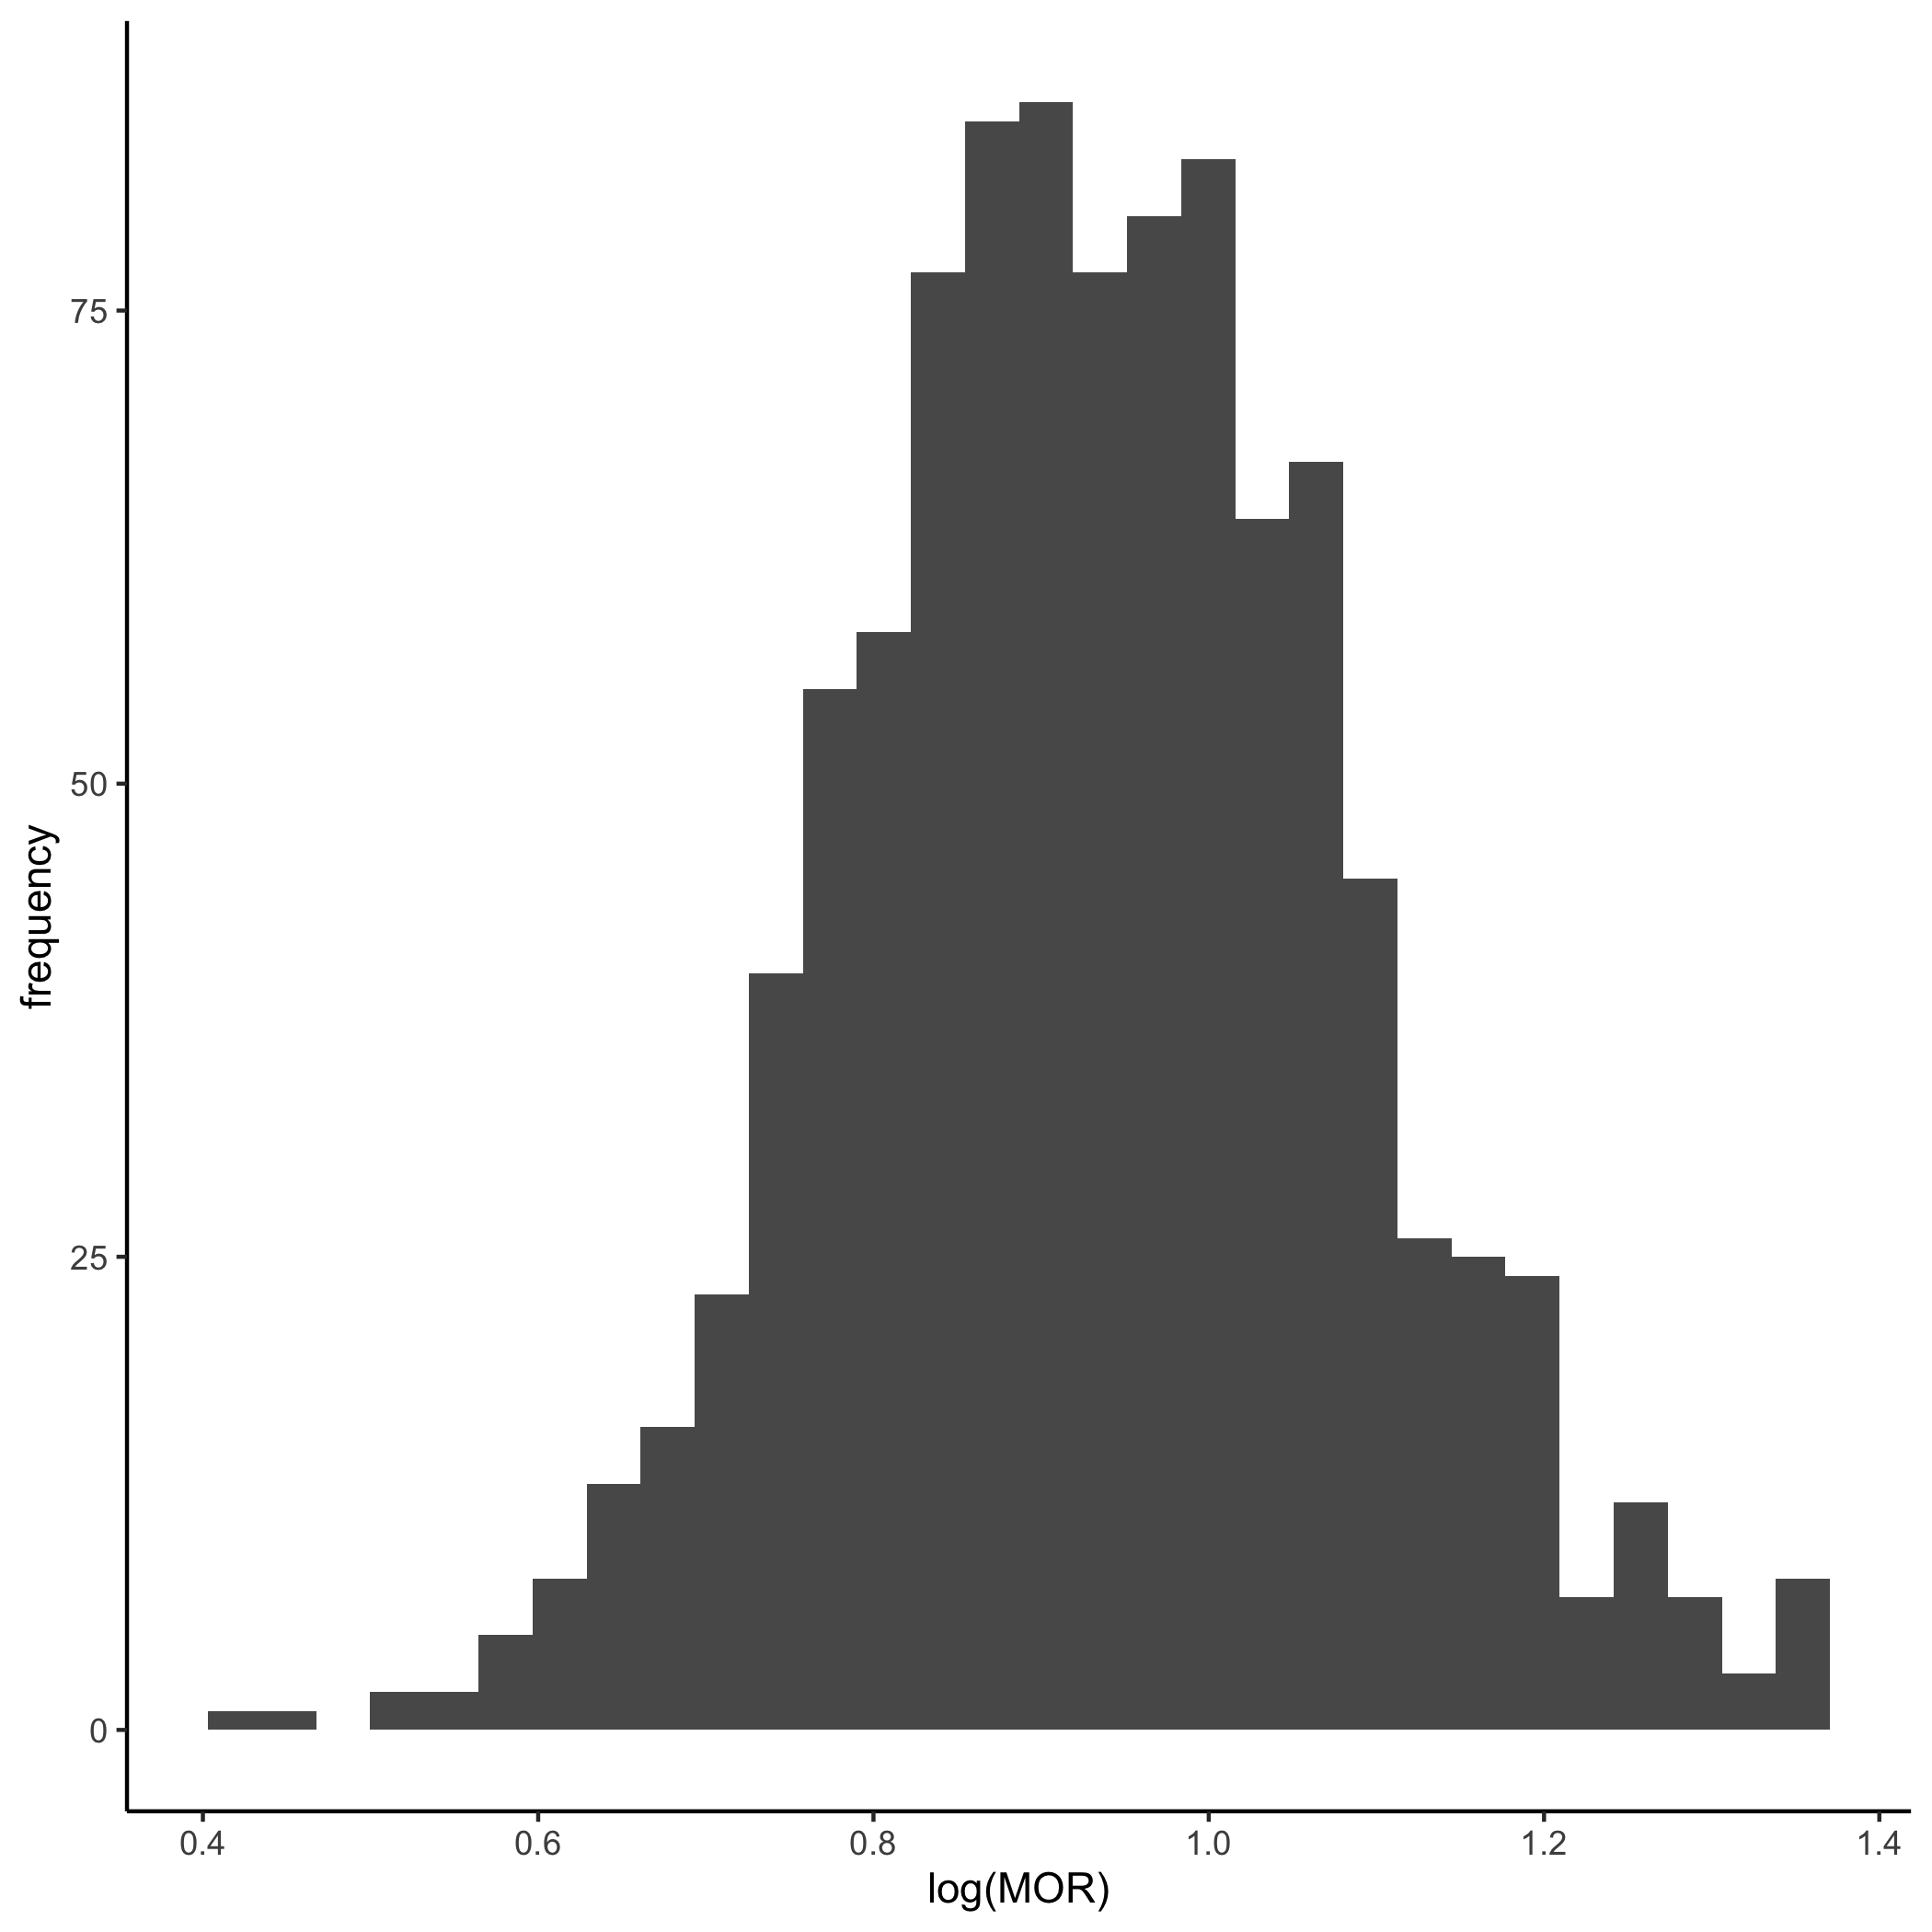
\includegraphics{../../plots/two-lvl-ran-slope/high-prev/hist_50_30_two_lvl_slp_high_prev_q3.png}

}

\caption{Cluster size 30}

}

\end{minipage}%
%
\begin{minipage}[t]{0.24\linewidth}

{\centering 

\raisebox{-\height}{

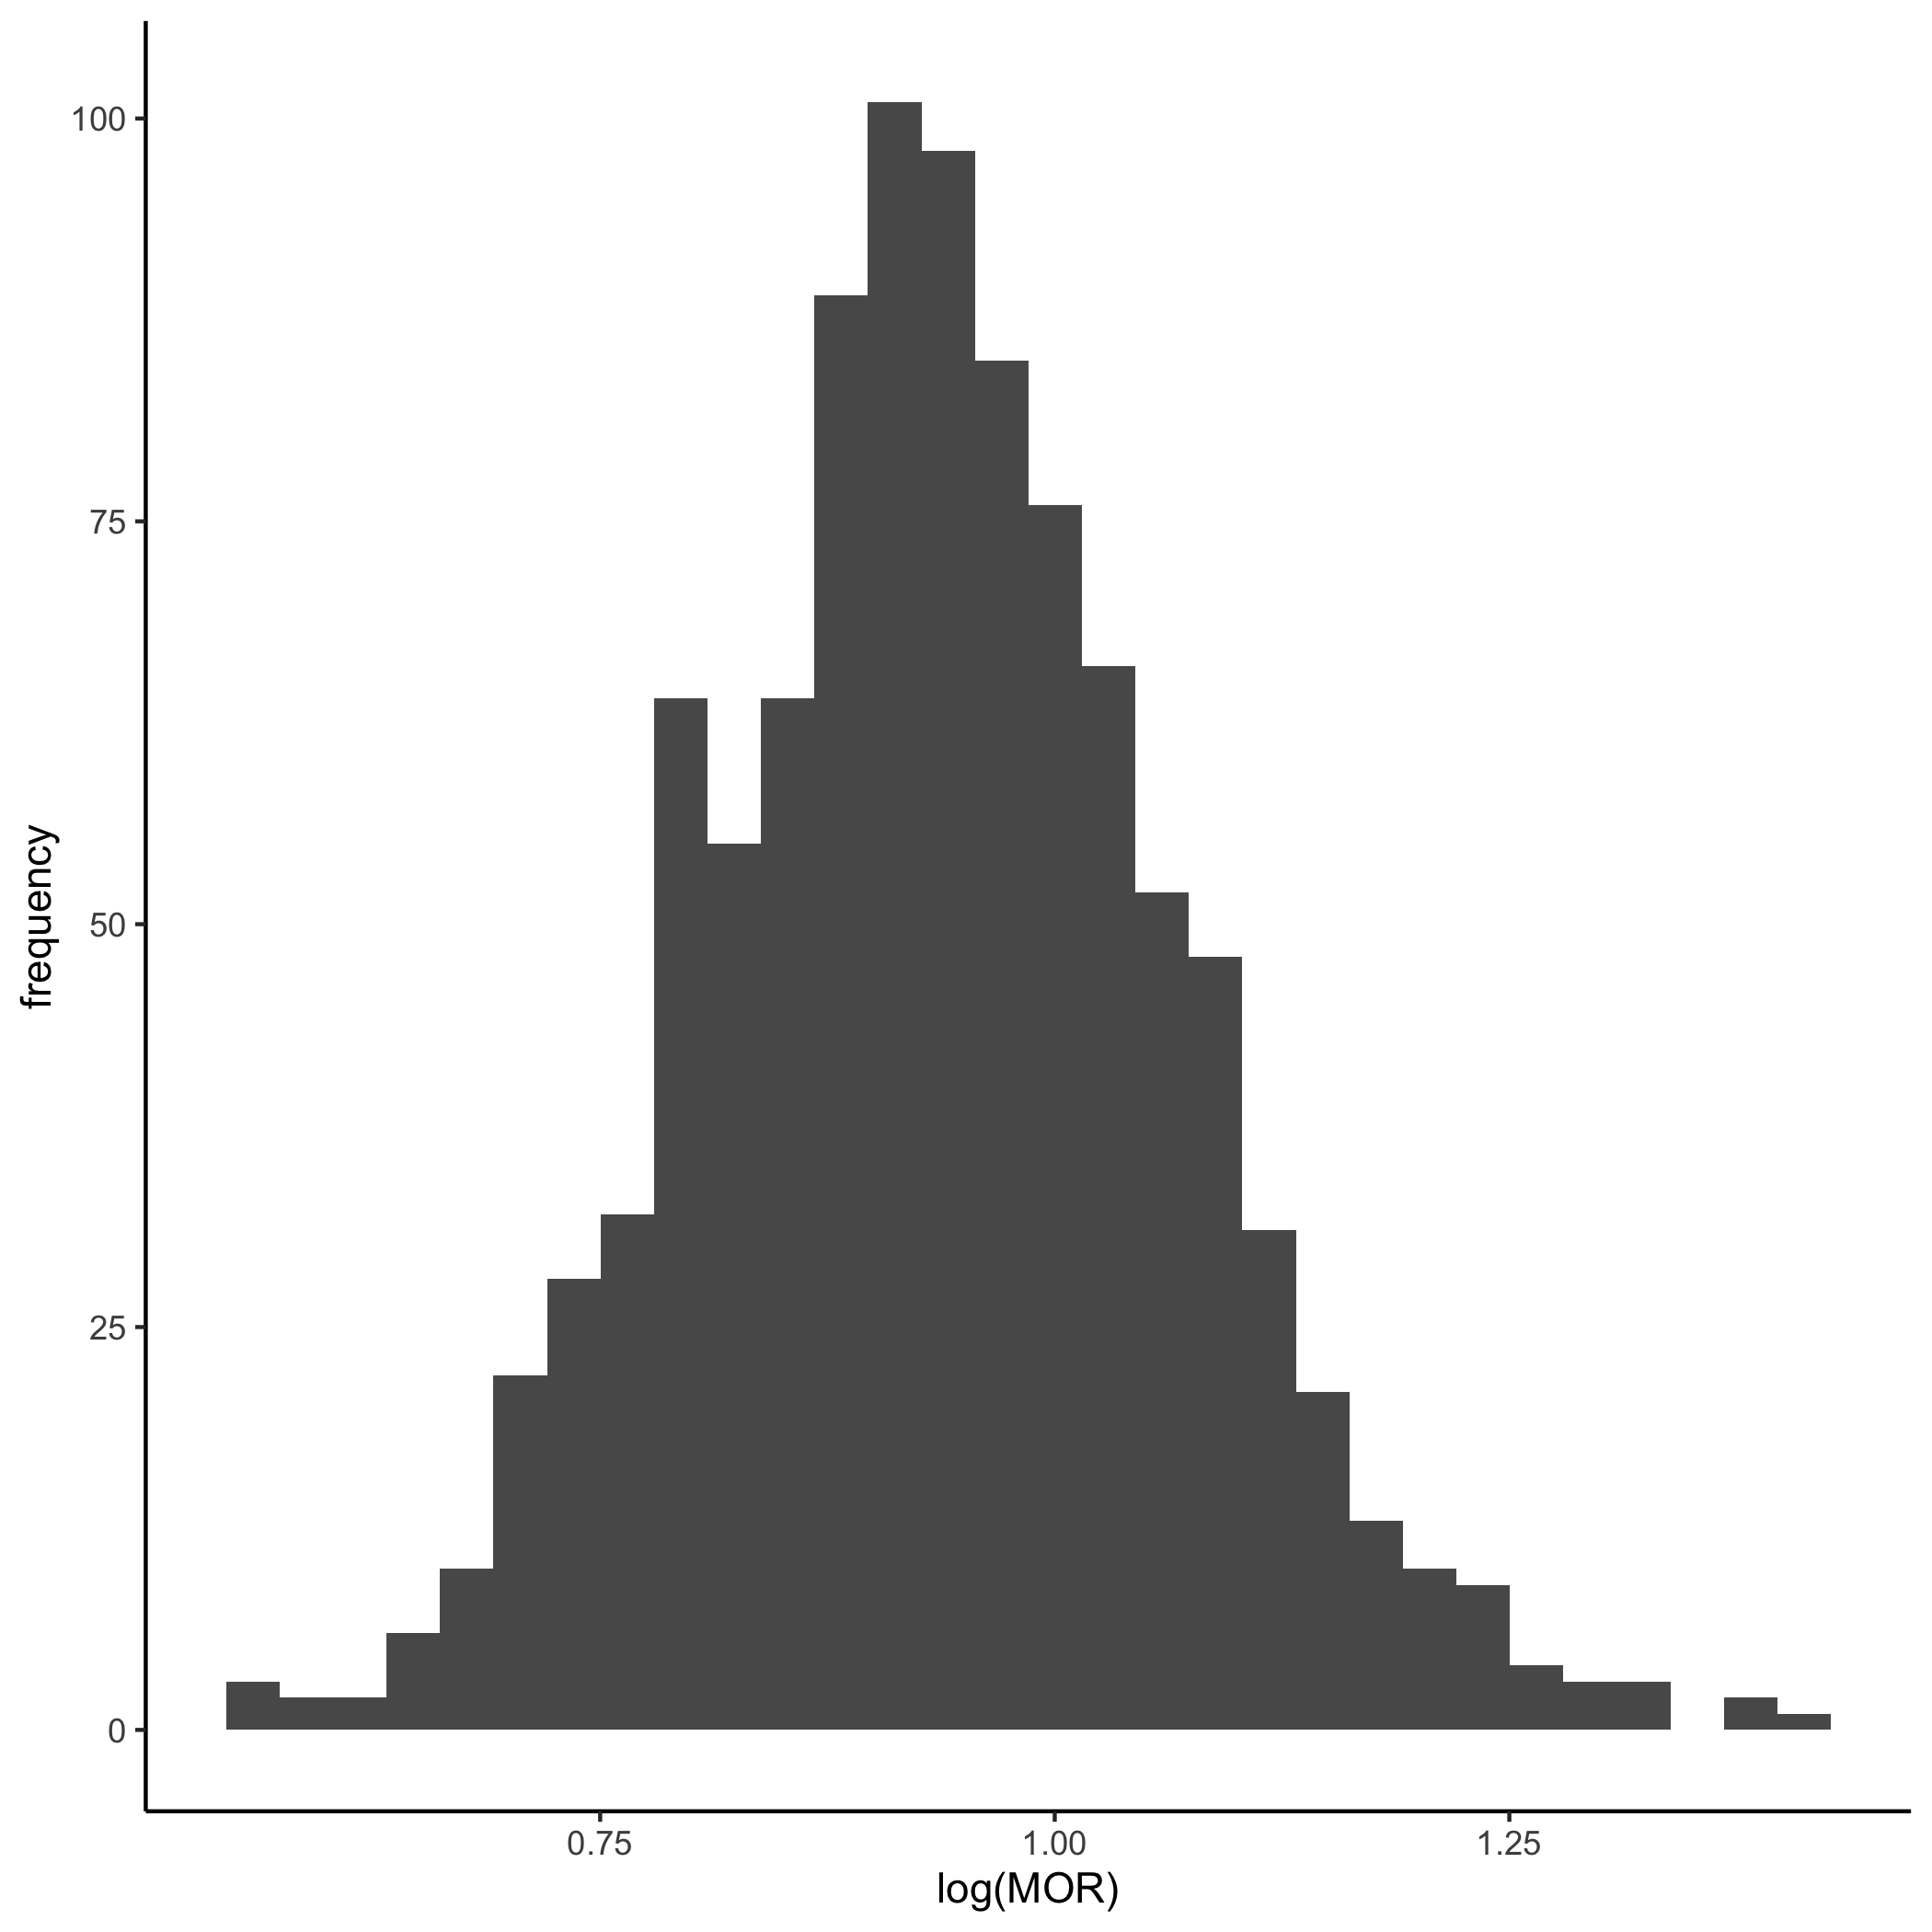
\includegraphics{../../plots/two-lvl-ran-slope/high-prev/hist_50_50_two_lvl_slp_high_prev_q3.png}

}

\caption{Cluster size 50}

}

\end{minipage}%
\newline
\begin{minipage}[t]{\linewidth}

{\centering 

~

}

\end{minipage}%
\newline
\begin{minipage}[t]{0.05\linewidth}

{\centering 

\rotatebox[origin=br]{90}{\tiny Cluster Number 100}

}

\end{minipage}%
%
\begin{minipage}[t]{0.24\linewidth}

{\centering 

\raisebox{-\height}{

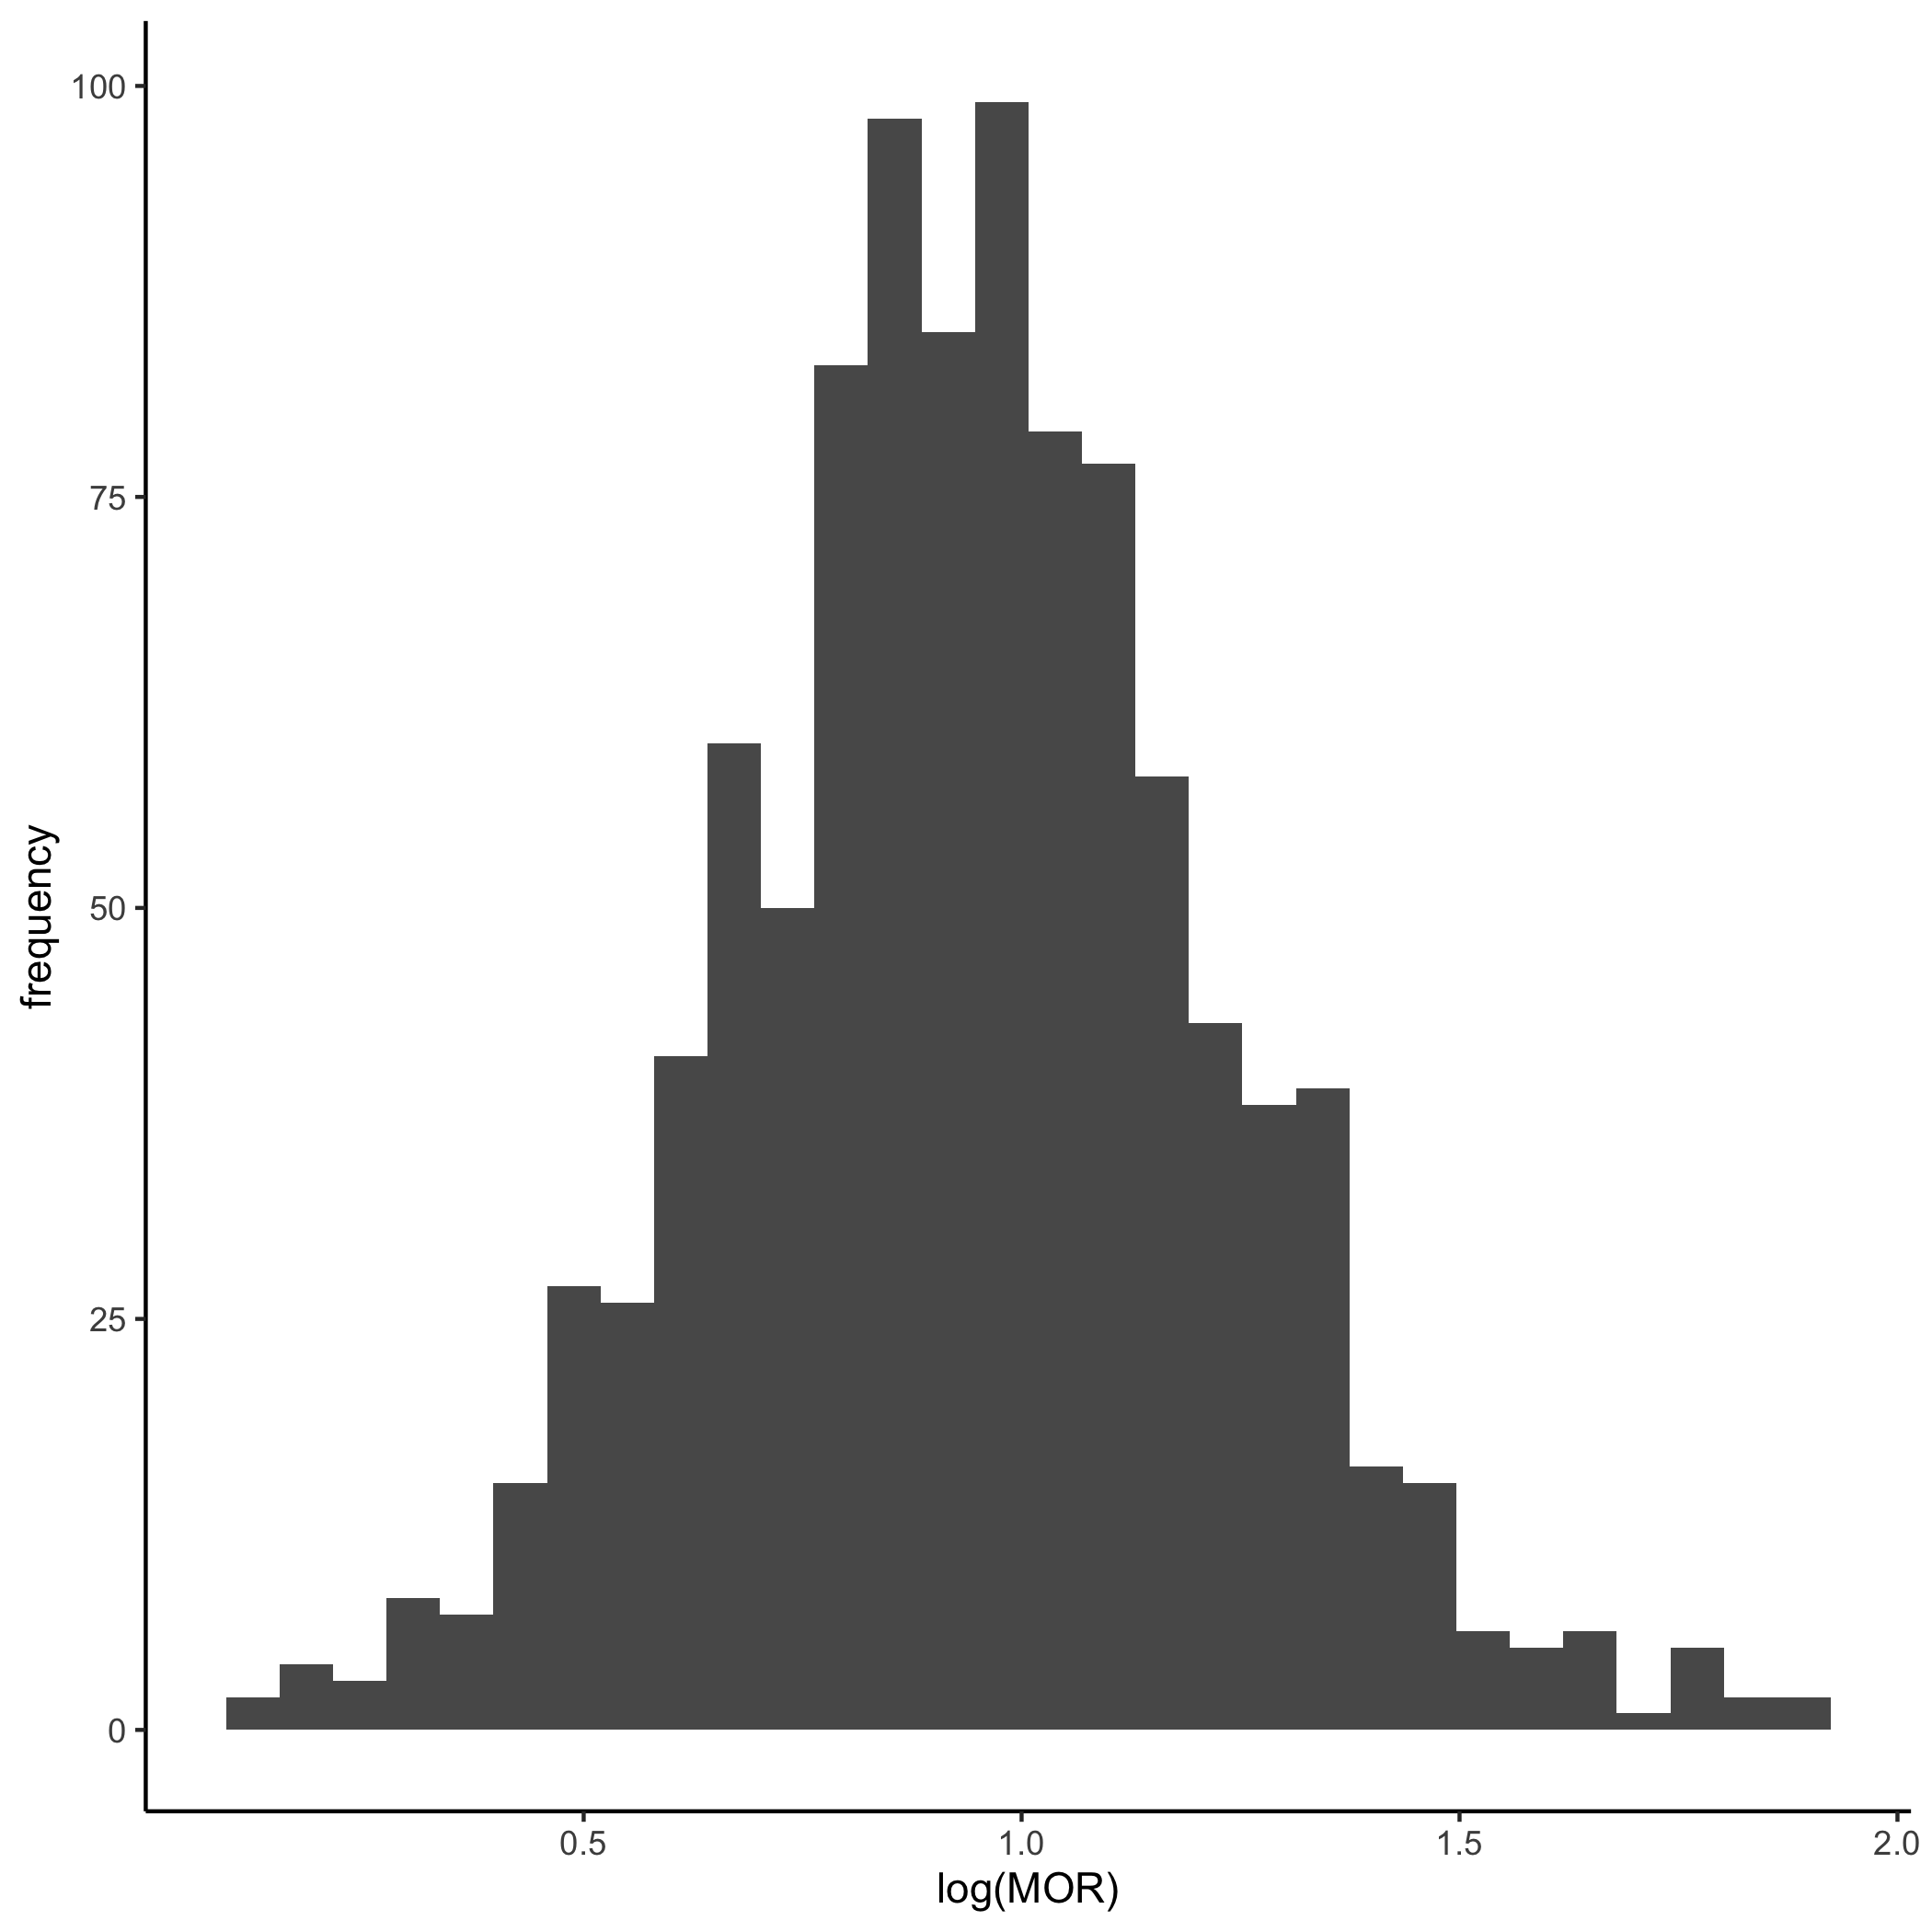
\includegraphics{../../plots/two-lvl-ran-slope/high-prev/hist_100_5_two_lvl_slp_high_prev_q3.png}

}

\caption{Cluster size 5}

}

\end{minipage}%
%
\begin{minipage}[t]{0.24\linewidth}

{\centering 

\raisebox{-\height}{

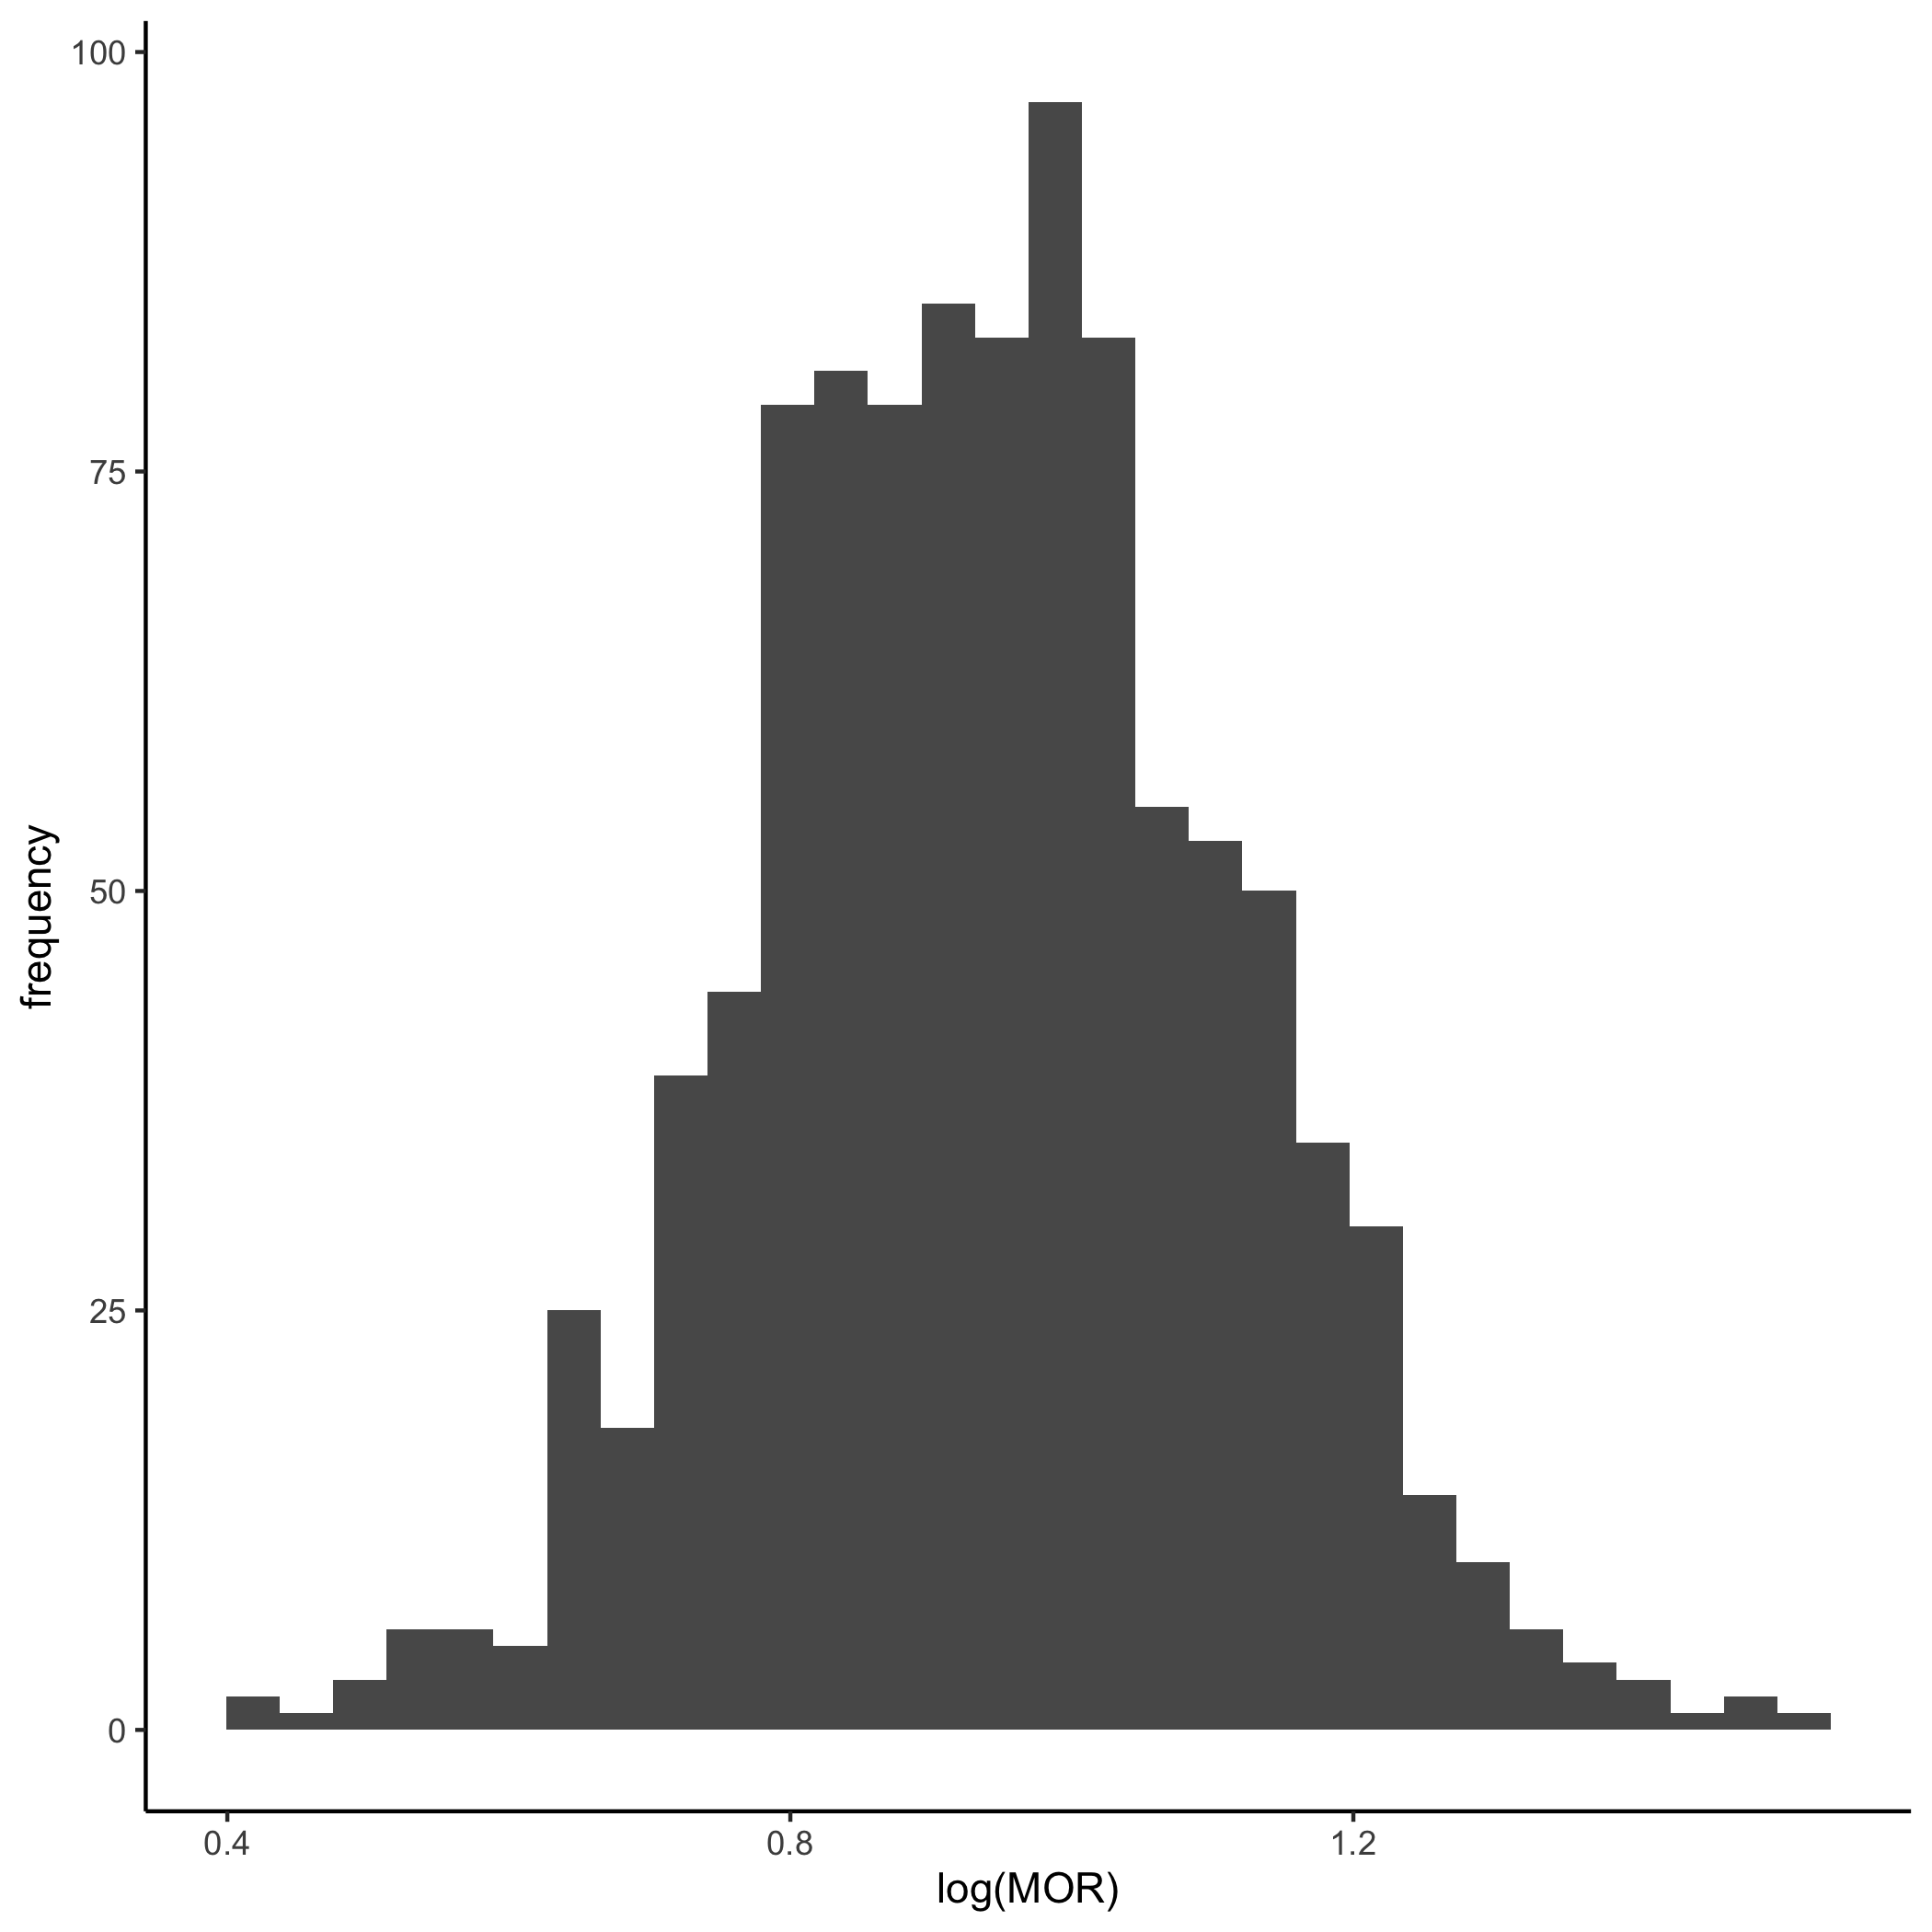
\includegraphics{../../plots/two-lvl-ran-slope/high-prev/hist_100_10_two_lvl_slp_high_prev_q3.png}

}

\caption{Cluster size 10}

}

\end{minipage}%
%
\begin{minipage}[t]{0.24\linewidth}

{\centering 

\raisebox{-\height}{

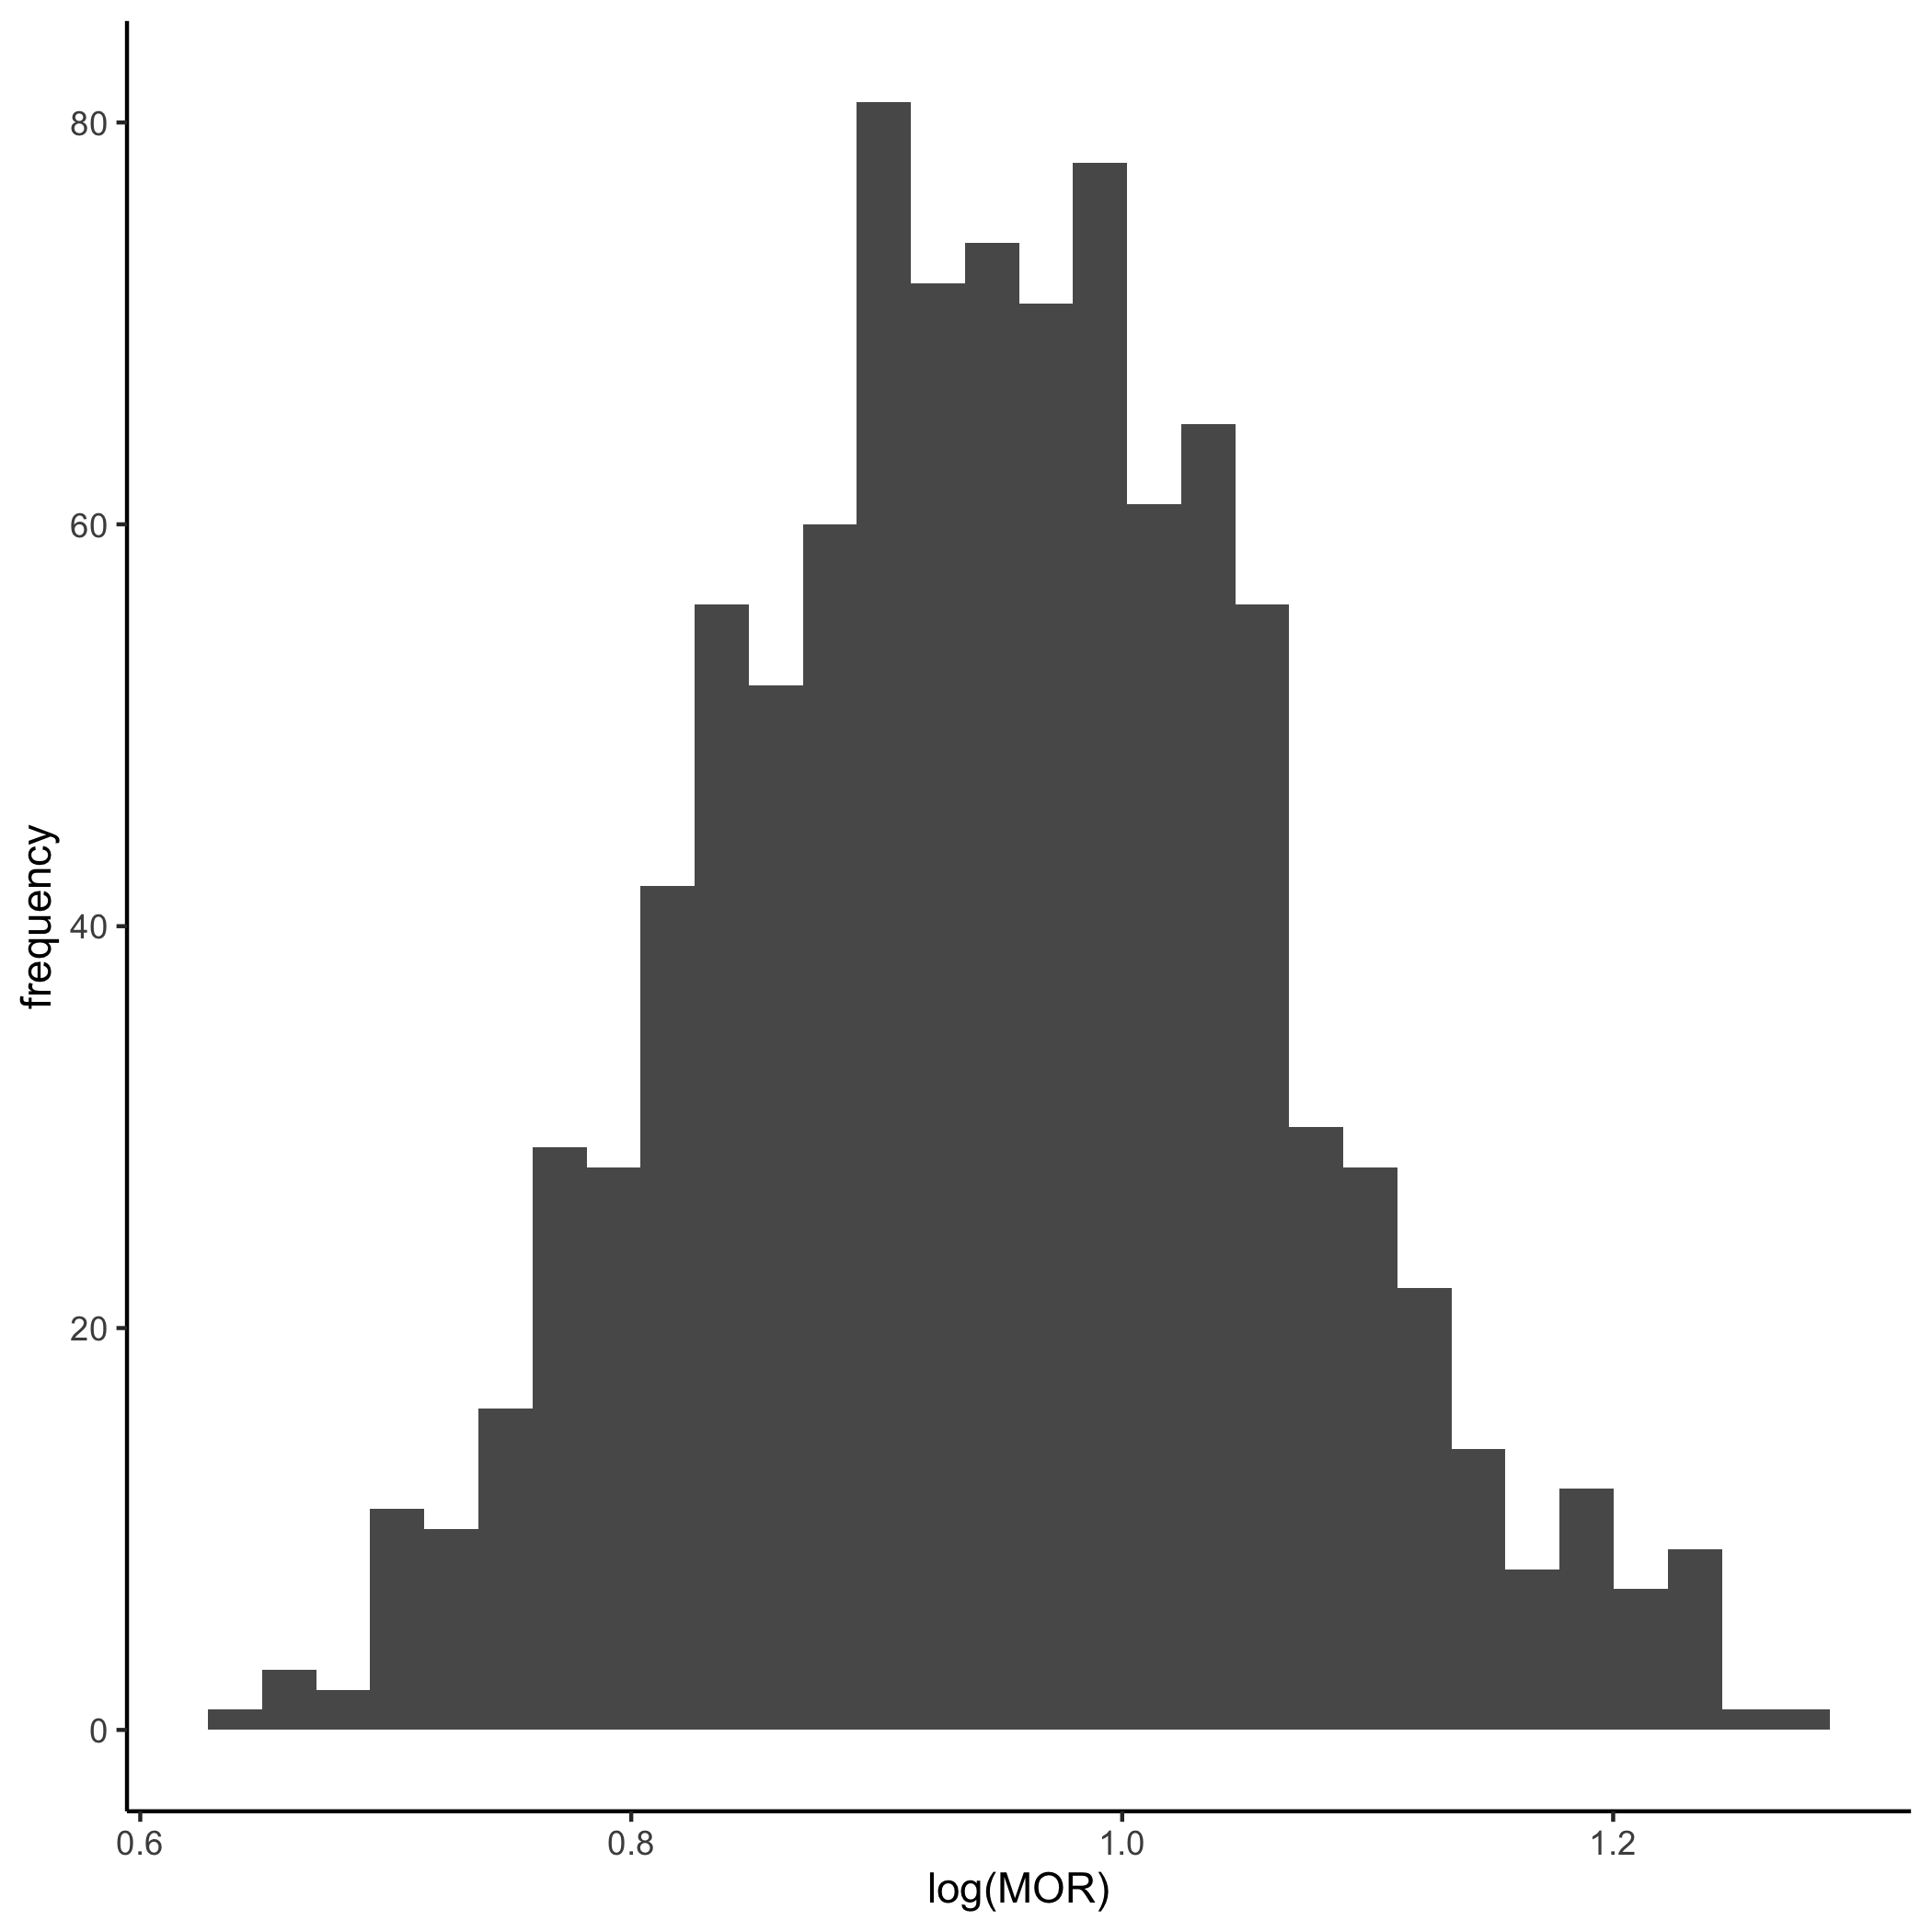
\includegraphics{../../plots/two-lvl-ran-slope/high-prev/hist_100_30_two_lvl_slp_high_prev_q3.png}

}

\caption{Cluster size 30}

}

\end{minipage}%
%
\begin{minipage}[t]{0.24\linewidth}

{\centering 

\raisebox{-\height}{

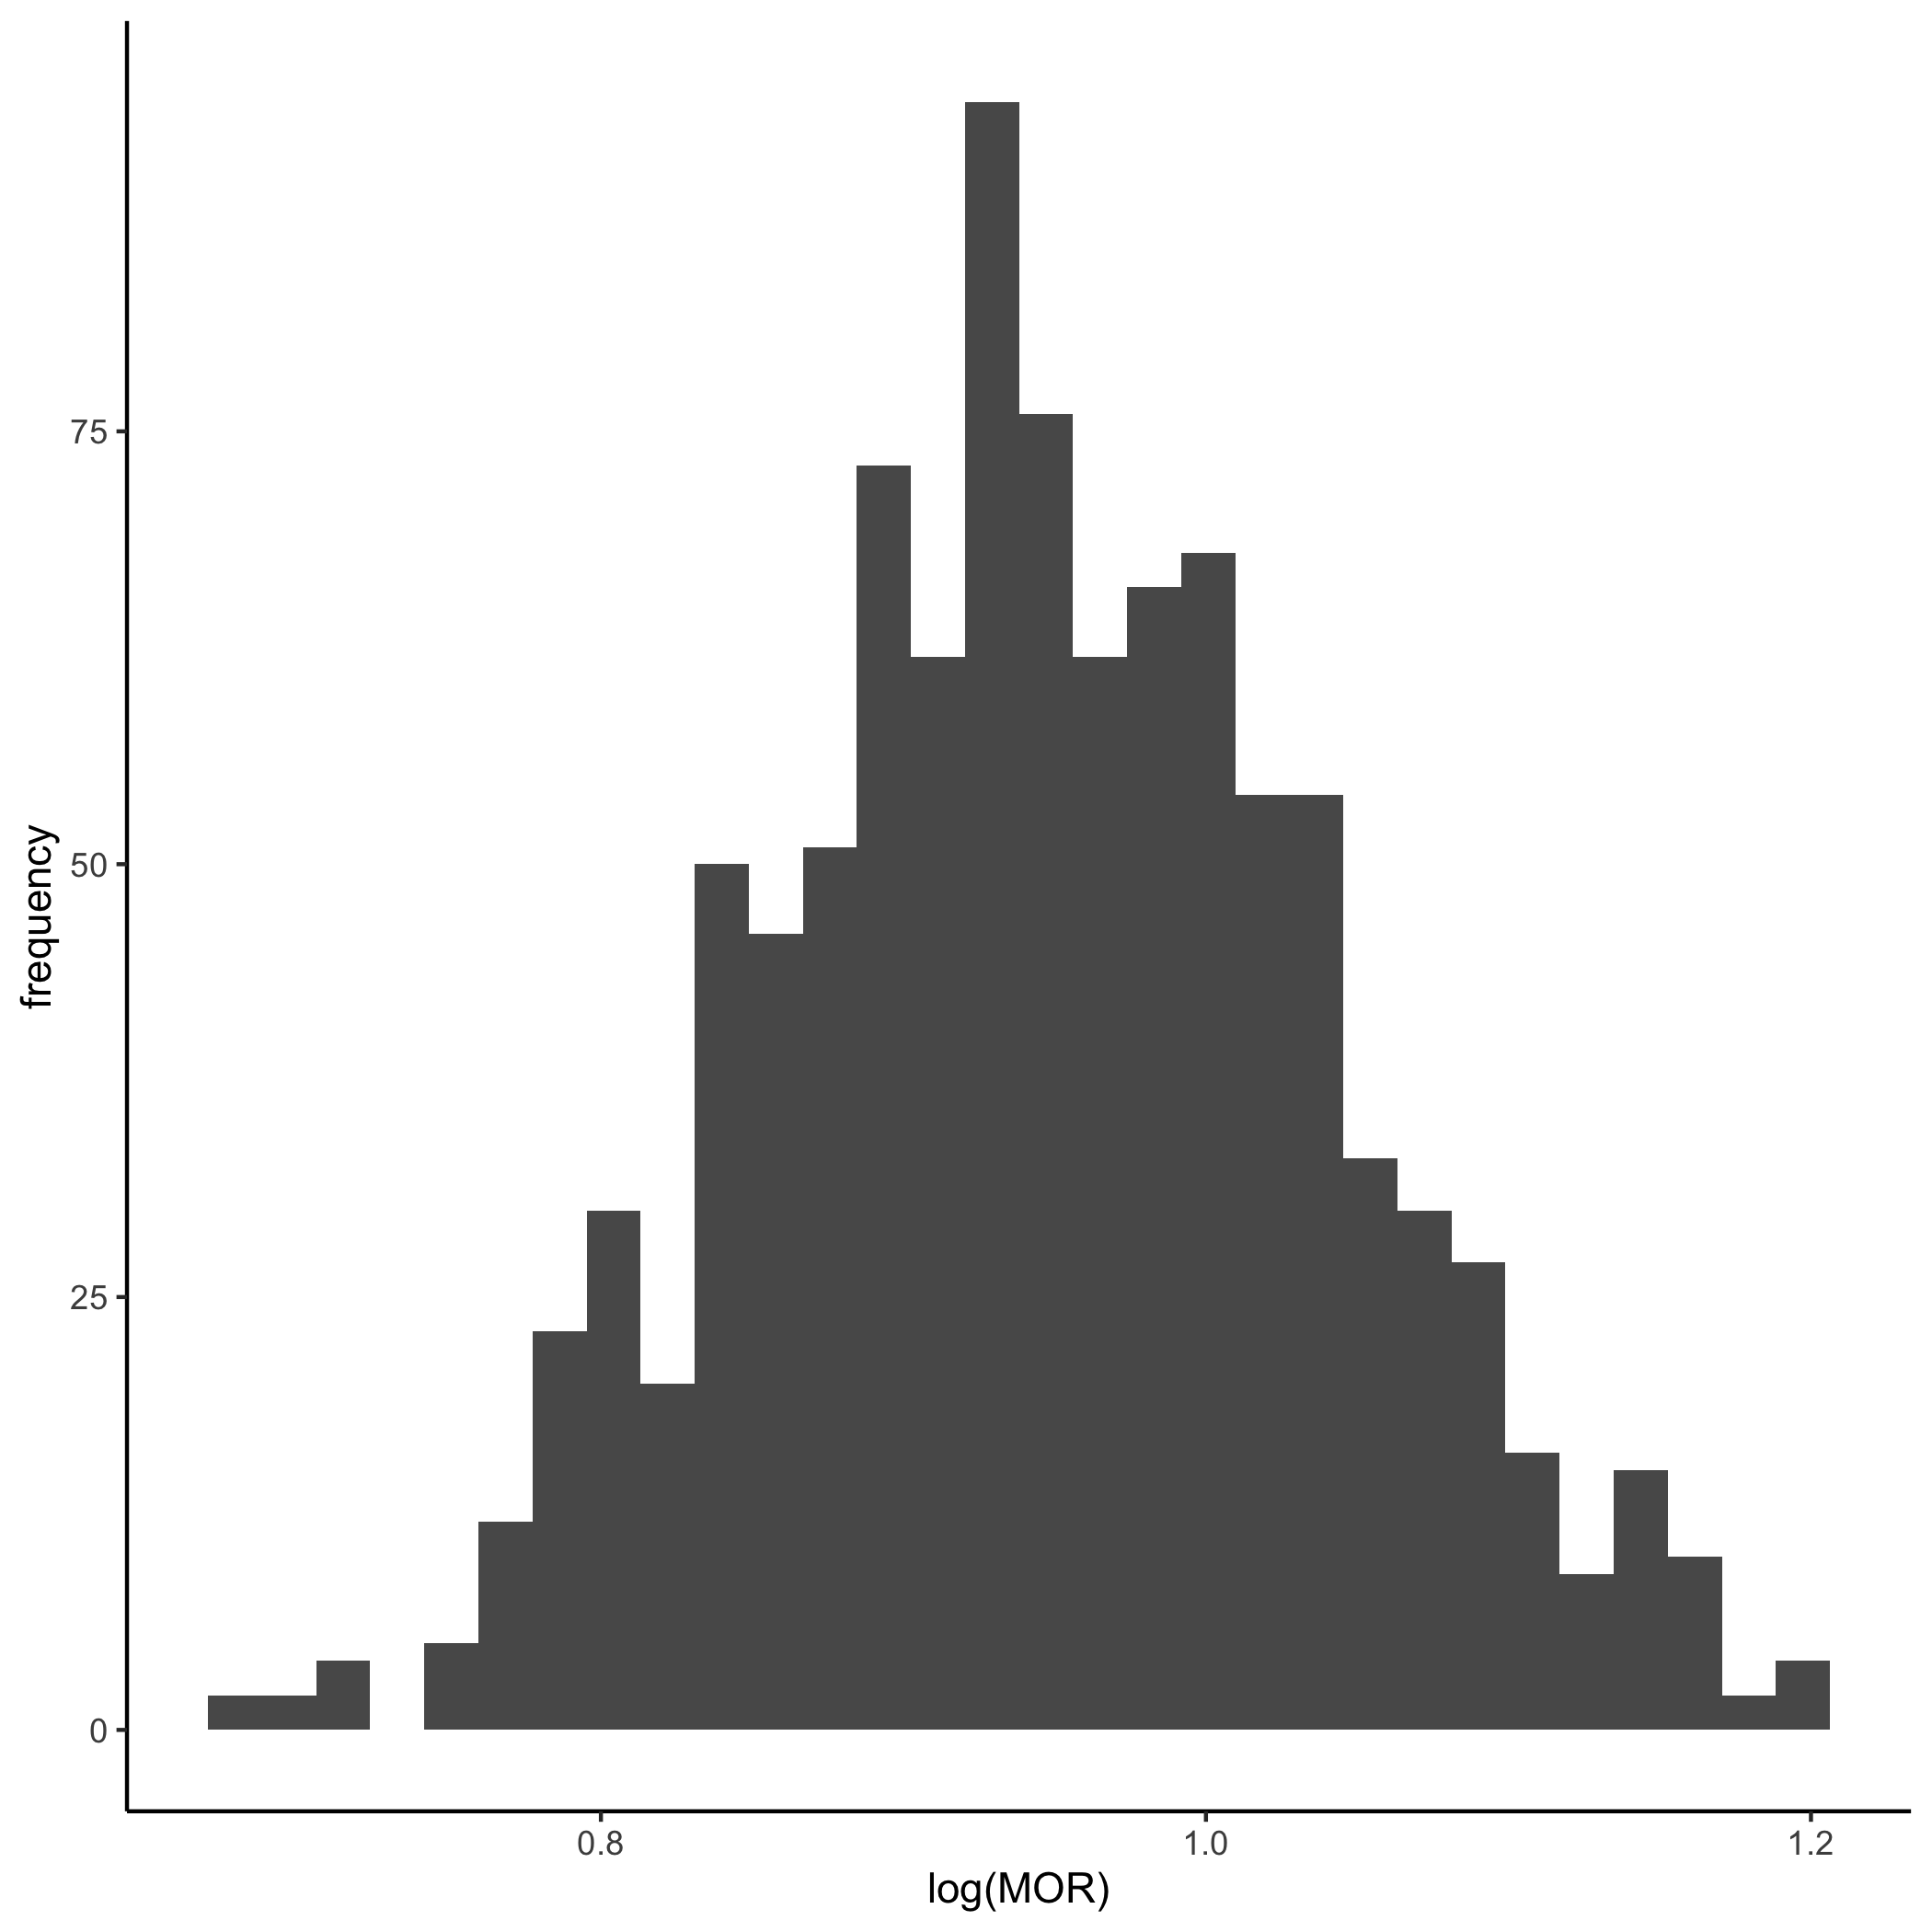
\includegraphics{../../plots/two-lvl-ran-slope/high-prev/hist_100_50_two_lvl_slp_high_prev_q3.png}

}

\caption{Cluster size 50}

}

\end{minipage}%

\end{figure}

\newpage

\KOMAoptions{usegeometry,paper=landscape,pagesize}
\recalctypearea
\newgeometry{right=10mm,left=10mm}

\hypertarget{simulation-result-table}{%
\section{Simulation Result Table}\label{simulation-result-table}}

\begingroup

\fontsize{10pt}{16pt}\selectfont
\addtolength{\tabcolsep}{0.1pt}

\begin{tabular}[t]{>{\centering\arraybackslash}m{2.5cm}>{\raggedleft\arraybackslash}m{2.5cm}>{\raggedleft\arraybackslash}m{2.5cm}>{\raggedleft\arraybackslash}m{2.5cm}>{\raggedleft\arraybackslash}m{2.5cm}>{\raggedleft\arraybackslash}m{2.5cm}>{\raggedleft\arraybackslash}m{2.5cm}>{\raggedleft\arraybackslash}m{2.5cm}>{\raggedleft\arraybackslash}m{2.5cm}}
\toprule
Number of Cluster & Cluster Size & $\widehat{\beta_0}$ & $\widehat{\beta_1}$ & $\widehat{\beta_2}$ & $\widehat{\sigma_{u_1}^2}$ & $\widehat{\sigma_{u_2}^2}$ & $\widehat{\sigma_{u_{12}}^2}$ & Model Convergence (\%)\\
\midrule
 & 5 & -1.90 & 1.88 & 0.65 & 1.26 & 2.37 & 0.10 & 60.10\\

 & 10 & -1.97 & 1.90 & 0.68 & 1.18 & 2.36 & 0.04 & 91.66\\

 & 30 & -1.89 & 1.79 & 0.68 & 0.98 & 1.95 & 0.04 & 99.60\\

\multirow{-4}{2.5cm}{\centering\arraybackslash 10} & 50 & -1.85 & 1.75 & 0.68 & 0.93 & 1.88 & 0.01 & 99.80\\
\cmidrule{1-9}
 & 5 & -1.95 & 1.83 & 0.71 & 1.23 & 2.40 & 0.04 & 97.09\\

 & 10 & -1.86 & 1.78 & 0.65 & 1.02 & 2.19 & 0.05 & 100.00\\

 & 30 & -1.85 & 1.75 & 0.67 & 0.97 & 1.98 & 0.00 & 100.00\\

\multirow{-4}{2.5cm}{\centering\arraybackslash 30} & 50 & -1.85 & 1.74 & 0.66 & 0.97 & 1.94 & 0.01 & 100.00\\
\cmidrule{1-9}
 & 5 & -1.91 & 1.83 & 0.68 & 1.15 & 2.34 & 0.06 & 99.80\\

 & 10 & -1.86 & 1.75 & 0.67 & 1.00 & 2.10 & 0.03 & 100.00\\

 & 30 & -1.85 & 1.74 & 0.67 & 0.98 & 1.98 & 0.02 & 100.00\\

\multirow{-4}{2.5cm}{\centering\arraybackslash 50} & 50 & -1.84 & 1.74 & 0.66 & 0.98 & 1.95 & 0.01 & 100.00\\
\cmidrule{1-9}
 & 5 & -1.85 & 1.74 & 0.66 & 1.06 & 2.08 & 0.05 & 99.90\\

 & 10 & -1.86 & 1.75 & 0.67 & 1.01 & 2.04 & 0.01 & 100.00\\

 & 30 & -1.85 & 1.75 & 0.67 & 1.00 & 1.99 & 0.01 & 100.00\\

\multirow{-4}{2.5cm}{\centering\arraybackslash 100} & 50 & -1.86 & 1.74 & 0.67 & 1.00 & 1.97 & 0.01 & 100.00\\
\bottomrule
\multicolumn{9}{l}{\rule{0pt}{1em}\textit{Note: }}\\
\multicolumn{9}{l}{\rule{0pt}{1em} }\\
\multicolumn{9}{l}{\rule{0pt}{1em}\textsuperscript{*} The mean prevalence for this simulation is 27\%}\\
\multicolumn{9}{l}{\rule{0pt}{1em}\textsuperscript{\dag} True $\sigma^2_{u_1}$ = $1$, $\sigma^2_{u_2}$ = $2$, $\sigma^2_{u_{12}}$ = $0$}\\
\multicolumn{9}{l}{\rule{0pt}{1em}\textsuperscript{\ddag} True Values of $\beta_0 = -1.85$, $\beta_1 = 1.75$, $\beta_2 = 0.67$}\\
\end{tabular}

\endgroup

\newpage

\hypertarget{simulation-result-table-when-first-quartile-of-x-is-used}{%
\section{Simulation Result Table When First Quartile of X is
used}\label{simulation-result-table-when-first-quartile-of-x-is-used}}

\begingroup

\fontsize{10pt}{14pt}\selectfont
\addtolength{\tabcolsep}{3pt}

\begin{tabular}[t]{>{\centering\arraybackslash}m{2.5cm}>{\raggedleft\arraybackslash}m{2.2cm}>{\raggedleft\arraybackslash}m{2.2cm}>{\raggedleft\arraybackslash}m{2.2cm}>{\raggedleft\arraybackslash}m{2.2cm}>{\raggedleft\arraybackslash}m{2.2cm}>{\raggedleft\arraybackslash}m{2.2cm}>{\raggedleft\arraybackslash}m{2.2cm}>{\raggedleft\arraybackslash}m{2.2cm}}
\toprule
Number of Cluster & Cluster Size & $MOR$ & $\widehat{MOR}$ & $Bias\textsuperscript{1}$ & $\widehat{SE}_{MOR}$ & Sim. $\widehat{SE}_{MOR}\textsuperscript{2}$ & Ratio\textsuperscript{3} & CI Coverage (95\%)\\
\midrule
 & 5 & 3.76 & 4.66 & 23.87 & 6.94 & 2.18 & 3.18 & 0.99\\

 & 10 & 3.75 & 4.52 & 20.44 & 3.64 & 2.03 & 1.79 & 0.99\\

 & 30 & 3.73 & 3.74 & 0.33 & 1.99 & 1.69 & 1.18 & 0.96\\

\multirow{-4}{2.5cm}{\centering\arraybackslash 10} & 50 & 3.74 & 3.64 & -2.50 & 1.65 & 1.57 & 1.05 & 0.95\\
\cmidrule{1-9}
 & 5 & 3.74 & 4.56 & 21.81 & 2.81 & 1.96 & 1.43 & 0.97\\

 & 10 & 3.73 & 3.88 & 3.99 & 1.69 & 1.61 & 1.05 & 0.97\\

 & 30 & 3.73 & 3.72 & -0.47 & 1.31 & 1.35 & 0.97 & 0.93\\

\multirow{-4}{2.5cm}{\centering\arraybackslash 30} & 50 & 3.74 & 3.67 & -1.76 & 1.26 & 1.28 & 0.99 & 0.93\\
\cmidrule{1-9}
 & 5 & 3.73 & 4.25 & 13.77 & 2.01 & 1.77 & 1.14 & 0.96\\

 & 10 & 3.74 & 3.83 & 2.22 & 1.42 & 1.48 & 0.96 & 0.95\\

 & 30 & 3.74 & 3.70 & -1.06 & 1.23 & 1.26 & 0.97 & 0.92\\

\multirow{-4}{2.5cm}{\centering\arraybackslash 50} & 50 & 3.74 & 3.69 & -1.32 & 1.19 & 1.21 & 0.99 & 0.94\\
\cmidrule{1-9}
 & 5 & 3.74 & 3.86 & 3.24 & 1.49 & 1.50 & 0.99 & 0.96\\

 & 10 & 3.73 & 3.78 & 1.17 & 1.25 & 1.29 & 0.97 & 0.94\\

 & 30 & 3.73 & 3.72 & -0.28 & 1.15 & 1.17 & 0.98 & 0.91\\

\multirow{-4}{2.5cm}{\centering\arraybackslash 100} & 50 & 3.74 & 3.70 & -0.87 & 1.13 & 1.15 & 0.99 & 0.93\\
\bottomrule
\multicolumn{9}{l}{\rule{0pt}{1em}\textit{Note: }}\\
\multicolumn{9}{l}{\rule{0pt}{1em} }\\
\multicolumn{9}{l}{\rule{0pt}{1em}\textsuperscript{1} It is Relative Bias = $\dfrac{\widehat{\theta} - \theta}{\theta} \times 100$}\\
\multicolumn{9}{l}{\rule{0pt}{1em}\textsuperscript{2} Simulation Standard Error of $MOR$}\\
\multicolumn{9}{l}{\rule{0pt}{1em}\textsuperscript{3} Ratio$\;=\;\dfrac{\widehat{SE}_{MOR}}{Simulation\;\widehat{SE}_{MOR}}$}\\
\multicolumn{9}{l}{\rule{0pt}{1em}\textsuperscript{*} The mean prevalence for this simulation is 27\%}\\
\end{tabular}

\endgroup

\newpage

\hypertarget{simulation-result-table-when-second-quartile-of-x-is-used}{%
\section{Simulation Result Table When Second Quartile of X is
used}\label{simulation-result-table-when-second-quartile-of-x-is-used}}

\begingroup

\fontsize{10pt}{14pt}\selectfont
\addtolength{\tabcolsep}{3pt}

\begin{tabular}[t]{>{\centering\arraybackslash}m{2.5cm}>{\raggedleft\arraybackslash}m{2.2cm}>{\raggedleft\arraybackslash}m{2.2cm}>{\raggedleft\arraybackslash}m{2.2cm}>{\raggedleft\arraybackslash}m{2.2cm}>{\raggedleft\arraybackslash}m{2.2cm}>{\raggedleft\arraybackslash}m{2.2cm}>{\raggedleft\arraybackslash}m{2.2cm}>{\raggedleft\arraybackslash}m{2.2cm}}
\toprule
Number of Cluster & Cluster Size & $MOR$ & $\widehat{MOR}$ & $Bias\textsuperscript{1}$ & $\widehat{SE}_{MOR}$ & Sim. $\widehat{SE}_{MOR}\textsuperscript{2}$ & Ratio\textsuperscript{3} & CI Coverage (95\%)\\
\midrule
 & 5 & 2.64 & 3.06 & 15.73 & 3.00 & 1.87 & 1.61 & 0.99\\

 & 10 & 2.62 & 2.87 & 9.46 & 1.95 & 1.67 & 1.17 & 0.96\\

 & 30 & 2.60 & 2.57 & -1.24 & 1.42 & 1.44 & 0.99 & 0.90\\

\multirow{-4}{2.5cm}{\centering\arraybackslash 10} & 50 & 2.60 & 2.51 & -3.39 & 1.34 & 1.35 & 0.99 & 0.89\\
\cmidrule{1-9}
 & 5 & 2.61 & 2.93 & 12.39 & 1.75 & 1.63 & 1.07 & 0.98\\

 & 10 & 2.60 & 2.62 & 0.84 & 1.39 & 1.37 & 1.01 & 0.97\\

 & 30 & 2.60 & 2.56 & -1.41 & 1.21 & 1.23 & 0.99 & 0.92\\

\multirow{-4}{2.5cm}{\centering\arraybackslash 30} & 50 & 2.60 & 2.56 & -1.55 & 1.18 & 1.18 & 1.00 & 0.93\\
\cmidrule{1-9}
 & 5 & 2.61 & 2.81 & 7.72 & 1.51 & 1.46 & 1.04 & 0.97\\

 & 10 & 2.60 & 2.60 & -0.01 & 1.28 & 1.29 & 0.99 & 0.96\\

 & 30 & 2.60 & 2.58 & -0.82 & 1.16 & 1.16 & 1.00 & 0.94\\

\multirow{-4}{2.5cm}{\centering\arraybackslash 50} & 50 & 2.60 & 2.57 & -0.86 & 1.14 & 1.14 & 1.00 & 0.93\\
\cmidrule{1-9}
 & 5 & 2.60 & 2.68 & 2.95 & 1.33 & 1.33 & 1.00 & 0.97\\

 & 10 & 2.60 & 2.61 & 0.45 & 1.18 & 1.19 & 1.00 & 0.96\\

 & 30 & 2.60 & 2.60 & 0.00 & 1.11 & 1.12 & 0.99 & 0.92\\

\multirow{-4}{2.5cm}{\centering\arraybackslash 100} & 50 & 2.60 & 2.59 & -0.14 & 1.10 & 1.10 & 1.00 & 0.94\\
\bottomrule
\multicolumn{9}{l}{\rule{0pt}{1em}\textit{Note: }}\\
\multicolumn{9}{l}{\rule{0pt}{1em} }\\
\multicolumn{9}{l}{\rule{0pt}{1em}\textsuperscript{1} It is Relative Bias = $\dfrac{\widehat{\theta} - \theta}{\theta} \times 100$}\\
\multicolumn{9}{l}{\rule{0pt}{1em}\textsuperscript{2} Simulation Standard Error of $MOR$}\\
\multicolumn{9}{l}{\rule{0pt}{1em}\textsuperscript{3} Ratio$\;=\;\dfrac{\widehat{SE}_{MOR}}{Simulation\;\widehat{SE}_{MOR}}$}\\
\multicolumn{9}{l}{\rule{0pt}{1em}\textsuperscript{*} The mean prevalence for this simulation is 27\%}\\
\end{tabular}

\endgroup

\newpage

\hypertarget{simulation-result-table-when-third-quartile-of-x-is-used}{%
\section{Simulation Result Table When Third Quartile of X is
used}\label{simulation-result-table-when-third-quartile-of-x-is-used}}

\begingroup

\fontsize{10pt}{14pt}\selectfont
\addtolength{\tabcolsep}{3pt}

\begin{tabular}[t]{>{\centering\arraybackslash}m{2.5cm}>{\raggedleft\arraybackslash}m{2.2cm}>{\raggedleft\arraybackslash}m{2.2cm}>{\raggedleft\arraybackslash}m{2.2cm}>{\raggedleft\arraybackslash}m{2.2cm}>{\raggedleft\arraybackslash}m{2.2cm}>{\raggedleft\arraybackslash}m{2.2cm}>{\raggedleft\arraybackslash}m{2.2cm}>{\raggedleft\arraybackslash}m{2.2cm}}
\toprule
Number of Cluster & Cluster Size & $MOR$ & $\widehat{MOR}$ & $Bias\textsuperscript{1}$ & $\widehat{SE}_{MOR}$ & Sim. $\widehat{SE}_{MOR}\textsuperscript{2}$ & Ratio\textsuperscript{3} & CI Coverage (95\%)\\
\midrule
 & 5 & 3.74 & 5.04 & 34.39 & 6.10 & 1.87 & 3.26 & 1.00\\

 & 10 & 3.74 & 4.71 & 24.79 & 3.43 & 1.67 & 2.05 & 0.98\\

 & 30 & 3.75 & 3.88 & 3.44 & 1.72 & 1.44 & 1.20 & 0.96\\

\multirow{-4}{2.5cm}{\centering\arraybackslash 10} & 50 & 3.74 & 3.67 & -1.84 & 1.58 & 1.35 & 1.17 & 0.96\\
\cmidrule{1-9}
 & 5 & 3.75 & 4.67 & 24.52 & 2.66 & 1.63 & 1.63 & 0.98\\

 & 10 & 3.75 & 4.08 & 8.50 & 1.56 & 1.37 & 1.14 & 0.97\\

 & 30 & 3.75 & 3.73 & -0.36 & 1.30 & 1.23 & 1.06 & 0.97\\

\multirow{-4}{2.5cm}{\centering\arraybackslash 30} & 50 & 3.75 & 3.71 & -1.06 & 1.26 & 1.18 & 1.07 & 0.96\\
\cmidrule{1-9}
 & 5 & 3.75 & 4.45 & 18.80 & 1.79 & 1.46 & 1.22 & 0.96\\

 & 10 & 3.74 & 3.91 & 4.34 & 1.38 & 1.29 & 1.07 & 0.97\\

 & 30 & 3.75 & 3.76 & 0.27 & 1.22 & 1.16 & 1.05 & 0.97\\

\multirow{-4}{2.5cm}{\centering\arraybackslash 50} & 50 & 3.74 & 3.72 & -0.50 & 1.19 & 1.14 & 1.05 & 0.96\\
\cmidrule{1-9}
 & 5 & 3.74 & 4.02 & 7.47 & 1.42 & 1.33 & 1.07 & 0.96\\

 & 10 & 3.75 & 3.83 & 2.14 & 1.25 & 1.19 & 1.05 & 0.96\\

 & 30 & 3.74 & 3.76 & 0.45 & 1.15 & 1.12 & 1.03 & 0.95\\

\multirow{-4}{2.5cm}{\centering\arraybackslash 100} & 50 & 3.74 & 3.75 & 0.29 & 1.13 & 1.10 & 1.03 & 0.96\\
\bottomrule
\multicolumn{9}{l}{\rule{0pt}{1em}\textit{Note: }}\\
\multicolumn{9}{l}{\rule{0pt}{1em} }\\
\multicolumn{9}{l}{\rule{0pt}{1em}\textsuperscript{1} It is Relative Bias = $\dfrac{\widehat{\theta} - \theta}{\theta} \times 100$}\\
\multicolumn{9}{l}{\rule{0pt}{1em}\textsuperscript{2} Simulation Standard Error of $MOR$}\\
\multicolumn{9}{l}{\rule{0pt}{1em}\textsuperscript{3} Ratio$\;=\;\dfrac{\widehat{SE}_{MOR}}{Simulation\;\widehat{SE}_{MOR}}$}\\
\multicolumn{9}{l}{\rule{0pt}{1em}\textsuperscript{*} The mean prevalence for this simulation is 27\%}\\
\end{tabular}

\endgroup

\newpage

\hypertarget{simulation-result-table-all-together}{%
\section{Simulation Result Table (All
Together)}\label{simulation-result-table-all-together}}

\begingroup

\fontsize{7pt}{11pt}\selectfont
\addtolength{\tabcolsep}{-0.2pt}

\begin{tabular}[t]{>{\raggedright\arraybackslash}m{0.9cm}>{\raggedleft\arraybackslash}m{0.8cm}>{\raggedleft\arraybackslash}m{0.8cm}>{\raggedleft\arraybackslash}m{0.8cm}>{\raggedleft\arraybackslash}m{0.8cm}>{\raggedleft\arraybackslash}m{0.8cm}>{\raggedleft\arraybackslash}m{0.8cm}>{\raggedleft\arraybackslash}m{0.8cm}>{\raggedleft\arraybackslash}m{0.8cm}>{\raggedleft\arraybackslash}m{0.8cm}>{\raggedleft\arraybackslash}m{0.8cm}>{\raggedleft\arraybackslash}m{0.8cm}>{\raggedleft\arraybackslash}m{0.8cm}>{\raggedleft\arraybackslash}m{0.8cm}>{\raggedleft\arraybackslash}m{0.8cm}>{\raggedleft\arraybackslash}m{0.8cm}>{\raggedleft\arraybackslash}m{0.8cm}>{\raggedleft\arraybackslash}m{0.8cm}>{\raggedleft\arraybackslash}m{0.8cm}>{\raggedleft\arraybackslash}m{0.8cm}>{\raggedleft\arraybackslash}m{0.8cm}>{\raggedleft\arraybackslash}m{0.8cm}}
\toprule
\multicolumn{1}{c}{ } & \multicolumn{7}{c}{$Q_{1X}$} & \multicolumn{7}{c}{$Q_{2X}$} & \multicolumn{7}{c}{$Q_{3X}$} \\
\cmidrule(l{3pt}r{3pt}){2-8} \cmidrule(l{3pt}r{3pt}){9-15} \cmidrule(l{3pt}r{3pt}){16-22}
M, N\textsuperscript{1} & $MOR$ & $\widehat{MOR}$ & $Bias\textsuperscript{2}$ & $\widehat{SE}_{MOR}$ & Sim. $\widehat{SE}_{MOR}\textsuperscript{3}$ & Ratio\textsuperscript{3} & Coverage (95\%) & $MOR$ & $\widehat{MOR}$ & $Bias\textsuperscript{2}$ & $\widehat{SE}_{MOR}$ & Sim. $\widehat{SE}_{MOR}\textsuperscript{3}$ & Ratio\textsuperscript{3} & Coverage (95\%) & $MOR$ & $\widehat{MOR}$ & $Bias\textsuperscript{2}$ & $\widehat{SE}_{MOR}$ & Sim. $\widehat{SE}_{MOR}\textsuperscript{3}$ & Ratio\textsuperscript{3} & Coverage (95\%)\\
\midrule
10, 5 & 3.76 & 4.66 & 23.87 & 6.94 & 2.18 & 3.18 & 0.99 & 2.64 & 3.06 & 15.73 & 3.00 & 1.87 & 1.61 & 0.99 & 3.74 & 5.04 & 34.39 & 6.10 & 1.87 & 3.26 & 1.00\\
10, 10 & 3.75 & 4.52 & 20.44 & 3.64 & 2.03 & 1.79 & 0.99 & 2.62 & 2.87 & 9.46 & 1.95 & 1.67 & 1.17 & 0.96 & 3.74 & 4.71 & 24.79 & 3.43 & 1.67 & 2.05 & 0.98\\
10, 30 & 3.73 & 3.74 & 0.33 & 1.99 & 1.69 & 1.18 & 0.96 & 2.60 & 2.57 & -1.24 & 1.42 & 1.44 & 0.99 & 0.90 & 3.75 & 3.88 & 3.44 & 1.72 & 1.44 & 1.20 & 0.96\\
10, 50 & 3.74 & 3.64 & -2.50 & 1.65 & 1.57 & 1.05 & 0.95 & 2.60 & 2.51 & -3.39 & 1.34 & 1.35 & 0.99 & 0.89 & 3.74 & 3.67 & -1.84 & 1.58 & 1.35 & 1.17 & 0.96\\
\midrule
30, 5 & 3.74 & 4.56 & 21.81 & 2.81 & 1.96 & 1.43 & 0.97 & 2.61 & 2.93 & 12.39 & 1.75 & 1.63 & 1.07 & 0.98 & 3.75 & 4.67 & 24.52 & 2.66 & 1.63 & 1.63 & 0.98\\
30, 10 & 3.73 & 3.88 & 3.99 & 1.69 & 1.61 & 1.05 & 0.97 & 2.60 & 2.62 & 0.84 & 1.39 & 1.37 & 1.01 & 0.97 & 3.75 & 4.08 & 8.50 & 1.56 & 1.37 & 1.14 & 0.97\\
30, 30 & 3.73 & 3.72 & -0.47 & 1.31 & 1.35 & 0.97 & 0.93 & 2.60 & 2.56 & -1.41 & 1.21 & 1.23 & 0.99 & 0.92 & 3.75 & 3.73 & -0.36 & 1.30 & 1.23 & 1.06 & 0.97\\
30, 50 & 3.74 & 3.67 & -1.76 & 1.26 & 1.28 & 0.99 & 0.93 & 2.60 & 2.56 & -1.55 & 1.18 & 1.18 & 1.00 & 0.93 & 3.75 & 3.71 & -1.06 & 1.26 & 1.18 & 1.07 & 0.96\\
\midrule
50, 5 & 3.73 & 4.25 & 13.77 & 2.01 & 1.77 & 1.14 & 0.96 & 2.61 & 2.81 & 7.72 & 1.51 & 1.46 & 1.04 & 0.97 & 3.75 & 4.45 & 18.80 & 1.79 & 1.46 & 1.22 & 0.96\\
50, 10 & 3.74 & 3.83 & 2.22 & 1.42 & 1.48 & 0.96 & 0.95 & 2.60 & 2.60 & -0.01 & 1.28 & 1.29 & 0.99 & 0.96 & 3.74 & 3.91 & 4.34 & 1.38 & 1.29 & 1.07 & 0.97\\
50, 30 & 3.74 & 3.70 & -1.06 & 1.23 & 1.26 & 0.97 & 0.92 & 2.60 & 2.58 & -0.82 & 1.16 & 1.16 & 1.00 & 0.94 & 3.75 & 3.76 & 0.27 & 1.22 & 1.16 & 1.05 & 0.97\\
50, 50 & 3.74 & 3.69 & -1.32 & 1.19 & 1.21 & 0.99 & 0.94 & 2.60 & 2.57 & -0.86 & 1.14 & 1.14 & 1.00 & 0.93 & 3.74 & 3.72 & -0.50 & 1.19 & 1.14 & 1.05 & 0.96\\
\midrule
100, 5 & 3.74 & 3.86 & 3.24 & 1.49 & 1.50 & 0.99 & 0.96 & 2.60 & 2.68 & 2.95 & 1.33 & 1.33 & 1.00 & 0.97 & 3.74 & 4.02 & 7.47 & 1.42 & 1.33 & 1.07 & 0.96\\
100, 10 & 3.73 & 3.78 & 1.17 & 1.25 & 1.29 & 0.97 & 0.94 & 2.60 & 2.61 & 0.45 & 1.18 & 1.19 & 1.00 & 0.96 & 3.75 & 3.83 & 2.14 & 1.25 & 1.19 & 1.05 & 0.96\\
100, 30 & 3.73 & 3.72 & -0.28 & 1.15 & 1.17 & 0.98 & 0.91 & 2.60 & 2.60 & 0.00 & 1.11 & 1.12 & 0.99 & 0.92 & 3.74 & 3.76 & 0.45 & 1.15 & 1.12 & 1.03 & 0.95\\
100, 50 & 3.74 & 3.70 & -0.87 & 1.13 & 1.15 & 0.99 & 0.93 & 2.60 & 2.59 & -0.14 & 1.10 & 1.10 & 1.00 & 0.94 & 3.74 & 3.75 & 0.29 & 1.13 & 1.10 & 1.03 & 0.96\\
\bottomrule
\multicolumn{22}{l}{\rule{0pt}{1em}\textit{Note: }}\\
\multicolumn{22}{l}{\rule{0pt}{1em} }\\
\multicolumn{22}{l}{\rule{0pt}{1em}\textsuperscript{1} M is Number of Cluster and N is Cluster size}\\
\multicolumn{22}{l}{\rule{0pt}{1em}\textsuperscript{2} It is Relative Bias = $\dfrac{\widehat{\theta} - \theta}{\theta} \times 100$}\\
\multicolumn{22}{l}{\rule{0pt}{1em}\textsuperscript{3} Simulation Standard Error of $MOR$}\\
\multicolumn{22}{l}{\rule{0pt}{1em}\textsuperscript{4} Ratio$\;=\;\dfrac{\widehat{SE}_{MOR}}{Simulation\;\widehat{SE}_{MOR}}$}\\
\multicolumn{22}{l}{\rule{0pt}{1em}\textsuperscript{*} The mean prevalence for this simulation is 27\%}\\
\end{tabular}

\endgroup



\end{document}
